\documentclass[
12pt, % The default document font size, options: 10pt, 11pt, 12pt
%oneside, % Two side (alternating margins) for binding by default, uncomment to switch to one side
english, % ngerman for German
singlespacing, % Single line spacing, alternatives: onehalfspacing or doublespacing
%draft, % Uncomment to enable draft mode (no pictures, no links, overfull hboxes indicated)
%nolistspacing, % If the document is onehalfspacing or doublespacing, uncomment this to set spacing in lists to single
%liststotoc, % Uncomment to add the list of figures/tables/etc to the table of contents
%toctotoc, % Uncomment to add the main table of contents to the table of contents
%pax	rskip, % Uncomment to add space between paragraphs
%nohyperref, % Uncomment to not load the hyperref package
headsepline, % Uncomment to get a line under the header
%chapterinoneline, % Uncomment to place the chapter title next to the number on one line
%consistentlayout, % Uncomment to change the layout of the declaration, abstract and acknowledgements pages to match the default layout
]{MastersThesis} % The class file specifying the document structure

\usepackage[utf8]{inputenc} % Required for inputting international characters
\usepackage[T1]{fontenc} % Output font encoding for international characters

\usepackage{palatino} % Use the Palatino font by default

\usepackage[backend=bibtex,style=authoryear,natbib=true]{biblatex} % Use the bibtex backend with the authoryear citation style (which resembles APA)

\addbibresource{References.bib} % The filename of the bibliography
\usepackage{multirow}
\usepackage{amsmath}
\usepackage{amssymb}
\usepackage[autostyle=true]{csquotes} % Required to generate language-dependent quotes in the bibliography
\usepackage{graphicx}
\usepackage{subfigure}
%\usepackage{subcaption}


%----------------------------------------------------------------------------------------
%	MARGIN SETTINGS
%----------------------------------------------------------------------------------------

\geometry{
	paper=a4paper, % Change to letterpaper for US letter
	inner=3.0cm, % Inner margin
	outer=2.5cm, % Outer margin
	bindingoffset=.5cm, % Binding offset
	top=1.5cm, % Top margin
	bottom=1.5cm, % Bottom margin
	%showframe, % Uncomment to show how the type block is set on the page
}


%----------------------------------------------------------------------------------------
%	THESIS INFORMATION
%----------------------------------------------------------------------------------------
\thesistitle{Evaluation and improvement of a dual-channel method for detection and quantification of high-temperature events based on FireBIRD data} % Your thesis title, this is used in the title and abstract, print it elsewhere with \ttitle
\supervisor{Prof. Dr.-Ing. Uwe \textsc{Sörgel}\newline Dr.-Ing Plank \textsc{Plank}} % Your supervisor's name, this is used in the title page, print it elsewhere with \supname
\examiner{Prof. Dr.-Ing. Uwe \textsc{Sörgel}} % Your examiner's name, this is not currently used anywhere in the template, print it elsewhere with \examname
\degree{Master of Science} % Your degree name, this is used in the title page and abstract, print it elsewhere with \degreename
\author{Penghua \textsc{Li}} % Your name, this is used in the title page and abstract, print it elsewhere with \authorname
\addresses{} % Your address, this is not currently used anywhere in the template, print it elsewhere with \addressname

\subject{Remote Sensing} % Your subject area, this is not currently used anywhere in the template, print it elsewhere with \subjectname
\keywords{} % Keywords for your thesis, this is not currently used anywhere in the template, print it elsewhere with \keywordnames
\university{\href{https://www.uni-stuttgart.de}{Universität Stuttgart}} % Your university's name and URL, this is used in the title page and abstract, print it elsewhere with \univname
\department{\href{http://www.ifp.uni-stuttgart.de}{Institut für Photogrammetrie}} % Your department's name and URL, this is used in the title page and abstract, print it elsewhere with \deptname
\group{\href{http://www.ifp.uni-stuttgart.de/forschung/Remote_Sensing/index.en.html}{Remote Sensing}} % Your research group's name and URL, this is used in the title page, print it elsewhere with \groupname
\faculty{\href{http://www.geoengine.uni-stuttgart.de/}{Geomatics Engineering}} % Your faculty's name and URL, this is used in the title page and abstract, print it elsewhere with \facname

\AtBeginDocument{
\hypersetup{pdftitle=\ttitle} % Set the PDF's title to your title
\hypersetup{pdfauthor=\authorname} % Set the PDF's author to your name
\hypersetup{pdfkeywords=\keywordnames} % Set the PDF's keywords to your keywords
}

\begin{document}

\frontmatter % Use roman page numbering style (i, ii, iii, iv...) for the pre-content pages

\pagestyle{plain} % Default to the plain heading style until the thesis style is called for the body content


%----------------------------------------------------------------------------------------
%	TITLE PAGE
%----------------------------------------------------------------------------------------

\newgeometry{left=1.3cm,right=2.3cm, top=1.5cm, bottom=1.5cm}

\begin{titlepage}

\begin{minipage}[c][\textheight][t]{\textwidth}
  \centering
  \begin{minipage}[c]{2cm}%
    
\includegraphics[height=2cm]{ifp.png}%
  \end{minipage}
  \hfill
  \begin{minipage}[c]{8cm}
    \centering
    \vspace*{2mm}
    \LARGE Universität Stuttgart \\[3mm]
    \Large Institut für Photogrammetrie
  \end{minipage}
  \hfill
  \begin{minipage}[c]{2cm}%
    
\includegraphics[height=2cm]{logo_uni-stuttgart}%
  \end{minipage}\\[5mm]
  \rule{\textwidth}{0.5pt}\\[10mm]

%  \vspace*{2cm} % kein Bild: diese Zeile "einkommentieren" ...
  \vspace*{1cm} % ... und diese "auskommentieren ..."
  {\LARGE {Evaluation and improvement of a dual-channel method for detection and quantification of high-temperature events based on FireBIRD data}}\\
  \vspace*{1cm} % ... und diese "auskommentieren" ...

%  \vspace*{4cm} % kein Bild: diese Zeile "einkommentieren" ...
  
\includegraphics[height=6cm]{Geo_logo.jpg}\\[10mm] % ... und diese "auskommentieren"

  \vfill

  \Large Studienarbeit im Studiengang\\[2mm]
  \textbf{Geomatics Engineering}\\[2mm]
  an der Universität Stuttgart \\[10mm]
  Penghua Li\\[10mm]
	  Stuttgart, May {\the\year}\\[5mm]
  \rule{\textwidth}{0.5pt}\\[5mm]
  \begin{minipage}{\textwidth}%
  \hfill
  \begin{minipage}[t]{0.13\textwidth}%
  \large\textbf{Superviser:}\\ \\[3mm]%
  \large\textbf{Examer:}
  \end{minipage}
  \quad
  \begin{minipage}[t][3.0cm]{0.7\textwidth}%
    \large Dr.-Ing. Simon Manuel Plank\\
    Deutsches Zentrum für Luft- und Raumfahrt (DLR)\\[3mm]
    Prof. Dr.-Ing. Uwe Sörge\\
    Universität Stuttgart%\\[3mm]
%    PD Dr.-Ing. Kunz Heinzelmann\\
%    Polytechnicum Oberstett
  \end{minipage}
  \hfill
  \end{minipage}
\end{minipage}

\end{titlepage}
\restoregeometry
\cleardoublepage

%----------------------------------------------------------------------------------------
%	ABSTRACT PAGE
%----------------------------------------------------------------------------------------
\begin{abstract}
\addchaptertocentry{\abstractname}% Add the abstract to the table of contents
High-temperature events, such as fire hazards and volcanic eruptions, occur all over the world and influent the Earth's environment on global to local scales. However, the lack of practical  monitoring and understanding of the high-temperature events leads a number of problems. The FireBIRD mission of DLR aims to an effective monitoring and fully understanding of these events.\\

\noindent In this thesis, a competitive method called MITIP for detection and quantification of high-temperature events is introduced. It provides surface temperature and radiance maps and high-temperature events monitoring products using FireBIRD data. A fully investigation and evaluation of its performance is implemented and an improvement of the MITIP method is also included. Products of the MITIP method and comparison of them with the results of Zhukov's algorithm, which is used to process the FireBIRD data originally, is presented.\\


\noindent \textbf{Key words: high-temperature events, FireBIRD, MITIP, TET-1, hot spots}
\end{abstract}

%----------------------------------------------------------------------------------------
%	LIST OF CONTENTS/FIGURES/TABLES PAGES
%----------------------------------------------------------------------------------------

\tableofcontents % Prints the main table of contents

\listoffigures

\listoftables

%----------------------------------------------------------------------------------------
%	ABBREVIATIONS
%----------------------------------------------------------------------------------------

\begin{abbreviations}{ll} % Include a list of abbreviations (a table of two columns)
\textbf{AOI} & \textbf{A}rea \textbf{O}f \textbf{I}nterest \\
\textbf{BIRD} & \textbf{Bi}spectral \textbf{I}nfrared \textbf{D}etection \\
\textbf{BIROS} & \textbf{B}erlin \textbf{I}nfra\textbf{R}ed \textbf{O}ptical \textbf{S}ystem \\
\textbf{DEM} & \textbf{D}igital \textbf{E}levation \textbf{M}ap \\
\textbf{EM} & \textbf{E}lectro\textbf{M}agnetic \\
\textbf{FireBIRD} & \textbf{F}ire \textbf{R}ecognition with \textbf{Bi}-spectral \textbf{I}nfra\textbf{R}ed \textbf{D}etector \\
\textbf{FRP} & \textbf{F}ire \textbf{R}adiative \textbf{P}ower \\
\textbf{GED} & \textbf{G}lobal \textbf{E}missivity \textbf{D}atabase \\
\textbf{LST} & \textbf{L}and \textbf{S}urface \textbf{T}emperature \\
\textbf{LWIR} & \textbf{L}ong-\textbf{W}avelength \textbf{I}nf\textbf{R}ed \\
\textbf{MIR} & \textbf{M}id-\textbf{I}nfra\textbf{R}ed \\
\textbf{MITIP} & Mid-\textbf{I}nfrared and \textbf{T}hermal infrared \textbf{I}mage \textbf{P}rocessing \\
\textbf{MODTRAN} & \textbf{MOD}erate resolution atmpshperic \textbf{TRAN}smission \\
\textbf{MWIR} & \textbf{M}id-\textbf{W}avelength \textbf{I}nfra\textbf{R}ed \\
\text{NASA} & \textbf{N}ational \textbf{A}eronautics and \textbf{S}pace \textbf{A}dministration \\
\textbf{NIR} & \textbf{N}ear-\textbf{I}nfra\textbf{R}ed \\
\textbf{HSRS} & \textbf{H}ot\textbf{S}pot \textbf{R}ecognition \textbf{S}ystem \\
\textbf{SST} & \textbf{S}ea \textbf{S}urface \textbf{T}emperature \\
\textbf{HTE} & \textbf{H}igh-\textbf{T}emperature \textbf{E}vent \\
\textbf{TET} & \textbf{T}echnology \textbf{E}xperimen\textbf{T} carrier \\
\textbf{TIR} & \textbf{T}hermal-\textbf{I}nfra\textbf{R}ed \\
\textbf{TOA} & \textbf{T}op-\textbf{O}f-\textbf{A}tmosphere \\
\textbf{WAOSS-B} & \textbf{W}ide-\textbf{A}ngle \textbf{O}ptoelectronic \textbf{S}tereo \textbf{S}canner \\

\end{abbreviations}

%----------------------------------------------------------------------------------------
%	ACKNOWLEDGEMENTS
%----------------------------------------------------------------------------------------

%\begin{acknowledgements}
%\addchaptertocentry{\acknowledgementname} % Add the acknowledgements to the table of contents
%\end{acknowledgements}

%----------------------------------------------------------------------------------------
%	THESIS CONTENT - CHAPTERS
%----------------------------------------------------------------------------------------

\mainmatter % Begin numeric (1,2,3...) page numbering

\pagestyle{thesis} % Return the page headers back to the "thesis" style
                                                                                                                                                                                                                                                                                                                                                                                                                                                                                                                                                                                                                                                                                                                                                                                                                                                                                                                                                                                                                                                                                                                                                                                                                                                                                                                                                                                                                                                                                                                                                                                                                                                                                                                                                                                                 
% Include the chapters of the thesis as separate files from the Chapters folder
% Uncomment the lines as you write the chapters

\chapter{Introduction}

\label{Chapter1}

% Define some commands to keep the formatting separated from the content 
\newcommand{\keyword}[1]{\textbf{#1}}
\newcommand{\tabhead}[1]{\textbf{#1}}
\newcommand{\code}[1]{\texttt{#1}}
\newcommand{\file}[1]{\texttt{\bfseries#1}}
\newcommand{\option}[1]{\texttt{\itshape#1}}

%----------------------------------------------------------------------------------------
%	SECTION 1
%----------------------------------------------------------------------------------------

\section{Introduction}

%-----------------------------------
%	SUBSECTION 1
%-----------------------------------

\subsection{Impacts of high-temperature events}

High Temperature Events (HTE), such as fire hazards and volcanic eruptions, occur widely all over the world and exert great impacts on the environment in both space and time domain from global to local scales. These HTEs, without doubt, play crucial roles for the environental equilibrium \parencite{Reference1}. HTEs might bring benefits at appropriate time and places, for example by speeding up the procedure of returning nutrients to the soils after vegetation senescence \parencite{Reference2}. However, the potentially hazardous characteristics of HTEs and the serious lack of knowledge about their fundamental roles in Earth system processes in the context of global climate change and population explosion will cause a multitude of problems \parencite{Reference3}.\\

\noindent Volcanoes represent a serious potential hazard for both the population and environment. Volcanic eruptions usually cause numerous loss of lives and damages to the surrounding environment \parencite{Reference12}. Besides the devastation caused by lava erupted, another significant and obvious effect of volcanic eruptions is the release of a host of gases and volcanic ashes, which might cause climate chage and serious air pollution. The 2010 eruptions of Eyjafjallajökull, a volcano in Iceland, although relatively small for volcanic eruptions, ejected a multitude of ashes into the atmosphere and created unprecedented disruptions to European air traffic during 15 - 20 April 2010, costing the aviation industry an estimated \$250 million per day \parencite{Reference4}. Furthermore, the population exposed to the eruption, had a higher prevalence of respiratory and mental symptoms \parencite{Reference5}.\\

\noindent Fire, another kind of high-temperature event, might be one of the most prevalent of all terrestrial disturbance agents for the modification of the Earth's surface and occurs worldwide \parencite{Reference6}. On one hand, fires in forests stimulate vegetation regeneration, increase plant biodiversity and optimize vegetation structure \parencite{Reference7}. On the other hand, fires, especially severe fires, can burn up vegetation and organics, resulting in hydrophobic layer on the soil surface or at certain depth of the soil, which makes the soil much more prone to be eroded by wind and rain and might lead to desertification in the end \parencite{Reference8}.\\

\noindent Due to the threats mentioned above, high-temperature events monitoring becomes more and more important. Besides, because of the huge areas affected by high-temperature events and its potentially dangerous characteristics, a critical role in the monitoring and investigating of HTE belongs to satellite remote sensing. Higher spatial and spectral resolution data is demanded to better detect and quantify high-temperature events.\\

%----------------------------------------------------------------------------------------
%	SUBSECTION 2
%----------------------------------------------------------------------------------------

\subsection{DLR's missions dedicated to high-temperature events monitoring}

The first DLR's satellite specially designed for HTE monitoring was the Bi-spectral InfraRed Detection (BIRD) satellite. The primary objective of the BIRD satellite was detection and quantitative analysis of high-temperature events like fires and volcanoes. The principal BIRD imaging payload includes the HotSpot Recognition System (HSRS) with one channel in Mid-InfraRed (MIR: 3.4 - 4.2$\mu$m) spectral range and one channel in Thermal-InfraRed (TIR: 8.5 - 9.3 $\mu$m) spectral range, the Wide-Angle Optoelectronic Stereo Scanner (WAOSS-B) with a nadir channel in Near-Infrared (NIR: 0.84 - 0.90$\mu$m) spectral range. The ground resolution was 185 meters in the NIR channel and 370 meters in the MIR and TIR channels \parencite{Reference9}.\\

\noindent Due to the success of the BIRD mission, DLR continues making efforts to HTE monitoring with the new Fire Recognition with Bi-spectral InraRed Detector (FireBIRD) mission. It consists of two small satellites Technology Experiment carrier (TET-1), launched in July 2012, and Berlin InfraRed Optical System (BIROS), launched in June 2016. Together, these two small satellites form the FireBIRD mini-constellation \parencite{Reference10}. Both of them carry a HSRS which is identical to BIRD. In addition, there are an additional 3-line VIS camera. Details about the sensors of TET-1 is shown in Table 1.\\

\begin{table}[!ht]
\caption{Main FireBIRD camera parameters (Altitude 510km) \parencite{Reference11}}
\centering
\begin{tabular} {l|l|l}
 \hline\hline
   & \textbf{3 line-VIS camera} & \textbf{2 infrared cameras} \\
 \hline
 \textbf{Wavelength} & Green: 460 - 560 nm  & MWIR: 3.4 - 4.2 $\mu$m \\
  & Red: 565 - 725 nm & LWIR: 8.5 - 9.3 $\mu$m \\
  & NIR: 790 - 930 nm & \\ 
 \hline
 \textbf{Focal length} & 90.9 mm & 46.39 mm \\
 \hline
 \textbf{FOV} & 19.6$^\circ$ & 19$^\circ$ \\
 \hline
 \textbf{Aperture (F-Number)} & 3.8 & 2.0 \\
 \hline
 \textbf{Detector} & CCD lines & CdHgTe arrays \\
 \hline
 \textbf{Pixel size} & 7 $\mu$m $\times$ 7 $\mu$m & 30 $\mu$m $\times$ 30 $\mu$m \\
 \hline
 \textbf{No. of pixel} & 3 $\times$ 5,164 & 2 $\times$ 512 staggered \\
 \hline
 \textbf{Quantization} & 14 bit & 14 bit \\
 \hline
 \textbf{Ground resolution} & 42.4 m & 356 m \\
 \hline
 \textbf{Sampling size} & 42.4 m & 178 m \\
 \hline
 \textbf{Swath width} & 211 km & 178 km \\
 \hline
 \textbf{In-flight calibration} & No & Black body flap \\
 \hline
 \textbf{Data rate} & max 44 MBit/s & 0.35 MBit/s \\
  & nom 11.2 Mbit/s & \\
 \hline
 \textbf{Accuracy} & 100 m at ground & 100 m at ground \\
 \hline\hline
\end{tabular}
\label{ParaFireBIRD}
\end{table}

\noindent Because BIROS is still undergoing an extensive testing program and does not put into use yet, the focus lies on TET-1 imageries in this thsis.\\ 

%----------------------------------------------------------------------------------------
%	SECTION 2
%----------------------------------------------------------------------------------------

\section{Outline of the thesis}
This thesis consist of six chapters. The remaining chapters are organized as follows.\\

\noindent Chapter 2 gives a brief intorduction of thermal infrared remote sensing, including the thermal infrared spectrum, atmospheric windows as well as some basic laws important for the quantitating fire pixels' characteristics. Furthermore, a practical and solid method for detection and characterization of sub-pixel fire and its pixel fraction is reviewed in section 2.2.\\

\noindent Then, a newly developed mehtod, called MITIP, which is used for atmospheric correction and thermal infrared image processing, is introducted in Chapter 3. The required input data for it and the necessary pre-processings are stated in section 3.1. Its procedures and principles, which are based on the theories and method introduced in Chapter2, are given in section 3.2. Section 3.3 gives a description of the outputs of the MITIP.\\

\noindent Chapter 4 presents the validation and improvements of the MITIP method. Its outputs are compared with the MODIS temperature products, namely MODIS Sea Surface Temperature (SST) and MODIS Land Surface Temperature (LST). These comparisons are done by means of time-series analyses for the purpose of further improvements of the MITIP method and finding suitable scale factors for the radiometric correction of TET-1 imageries. Finally, the calibration results are presented and the tests of the choosen scale factors for transferability with imageries of other test sites are shown as well.\\

\noindent In Chapter 5, the processing results of TET imageries of different test sites from the MITIP method are demostrated in section 5.1. The outcomes of the MITIP method and the results of Zhukov's algorithm, which is used to process TET-1 imageries originally, are compared in this chapter. In order to do the comparisons, a procedure is developed to convert the pixel-based results to cluster-based results, which is described in section 5.2. The comparison results are presented in section 5.3.\\

\noindent Finally, the conclusions and outlooks are given in Chapter 6.\\

\chapter{Theoretical background of thermal infrared remote sensing}

\label{Chapter2}

%description
%----------------------------------------------------------------------------------------
This chapter reviews some fundamentals of thermal remote sensing (Section 2.1), as well as a useful approach, which is also used in the MITIP method, to identify and determine target temperature of subpixle resolution (Section 2.2). \\

%----------------------------------------------------------------------------------------
%	SECTION 1
%----------------------------------------------------------------------------------------

\section{Principles of thermal infrared remote sensing}
Thermal remote sensing depends on the fact that any object with a temperature above absolute zero (0 K or -273.15 $^\circ$C) emits electromagnetic (EM) radiation in the infrared range. For example, the Earth we live has an average temperature around 300 K and its peak emittance is near 10 $\mu$m, which falls on thermal infrared (TIR) domain \parencite {Reference201, Reference202}. The spectral composition and intensity of the emited radiation are determined by its surface temperature, which is also called kinetic temperature $T_{kin}$,  and the emissivity of the object \parencite{Reference207}. The emissivity $\varepsilon_{\lambda}$, $\varepsilon$ for short, is a ratio of the radiant flux of an object at a certain temperature to the radiant flux of a blackbody at the same temperature (Equation \eqref{eq1}), representing the effectiveness of the object in emitting energy as thermal radiation. The blackbody is an idealized physical object that aborbs and re-emits all incident EM radiation, which means its emissivity is 1 \parencite{Reference206, Reference204}. The emissivity varies as a function of wavelength $\lambda$ and also depends on the surface type of the object, but is not temperature-dependent \parencite{Reference203}.\\
\begin{equation}
\label{eq1}
\varepsilon_{\lambda} = \frac{L_{gb, \lambda}(T_{kin})}{L_{gb, \lambda}(T_{kin})}
\end{equation}

\noindent with:\\
\indent $T_{kin}$ = kinetic temperature [K]\\
\indent $L_{gb, \lambda}(T_{kin})$ = radiance of an object with temperature $T_{kin}$ at a certain wavelength [$W m^{-2} sr^{-1} \mu m^{-1}$]\\
\indent $L_{bb, \lambda}(T_{kin})$ = radiance of blackbody with temperature $T_{kin}$ at a certain wavelength [$W m^{-2} sr^{-1} \mu m^{-1}$]\\

% Thus these sensors will produce thermal radiance images which record the equivalent blackbody radiances of the object on the Eearth's surface 
\noindent The satellite remote sensing snesors responsive in the thermal infrared domain are capable to record the EM radiations emited by Earth surface objects \parencite{Reference204}. With the recorded radiation the derivation of the radiant temperature $T_{rad}$ is possible. Radiant temperature $T_{rad}$ is the actual temperature obtained from the measurement of the sensor, representing temperature of a equivalent blackbody \parencite{Reference206}. Notice that the radiant temperature $T_{rad}$ and the kinematic temperature $T_{kin}$ are two different terms and the conversion between them will be introduced later.\\

%-----------------------------------
%	SUBSECTION 1
%-----------------------------------

\subsection{The thermal infrared domain and atmospheric windows}
There is no strict definition of the thermal infrared domain. Usually, the thermal infrared wavelength domain spread from around 3 to 14 $\mu$m. Within this range, there are two atomspheric windows in the 3 - 5 $\mu$m range and in the 8 - 14 $\mu$m range \parencite{Reference204}. \\

\begin{figure}[!htbp]
  \centering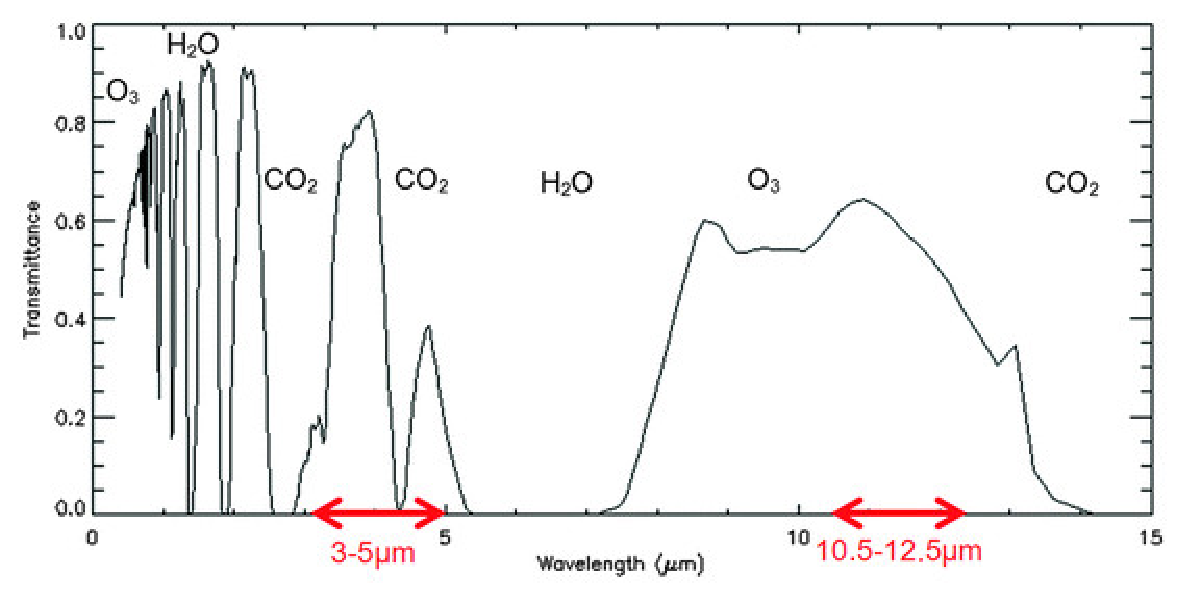
\includegraphics[width=0.8\textwidth]{The_thermal_infrared_wavelength_domain.eps}
  \caption{The thermal infrared wavelength domain \parencite{Reference204}.}
  \label{fig:TIRdomain}
\end{figure}

\noindent The spectrum range 8 - 14 $\mu$m, which is called Long-Wavelength InfRared (LWIR), is the thermal imaging region. Within this range, sensors are able to obtain a completely passive image based on the thermal radiation emitted by objects itself and no illumination required. There is only a absorption of OZone which is neglected by sensors. The sepectrum range 3 - 5 $\mu$m is called Mid-Wavelength InfraRed (MWIR). Sensors responsive to this specturm range will capture reflected sunlight which contaminates the object-emitted thermal signal. So More attention should be paid when dealing with day-time 3 - 5 $\mu$m MWIR imagery. \\

\noindent In this thesis, we focus on the night-time TET-1 scene only. \\

%-----------------------------------
%	SUBSECTION 2
%-----------------------------------

\subsection{The Planck's law and Stefan-Boltzmann law}
Planck's blackbody radiation law, Planck's law for short, describes the spectral density of electromagnetic radiation $B_{\lambda}(T_{kin})$ emitted by a blackbody at a given wavelength $\lambda$ as a function of the blackbody's absolute temperature \parencite{Reference208}. Given a certain wavelength $\lambda$, the spectral radiance $B_{\lambda}(T_{kin})$ can be computed from the body's temperature:
\begin{equation}
\label{eq2}
B_{\lambda}(T_{kin}) = L_{bb, \lambda}(T_{kin}) = \frac{2hc^2}{\lambda ^5} \frac{1}{e^{\frac{hc}{\lambda k T_{kin}}} - 1}
\end{equation}

\noindent with:\\
\indent $B_{\lambda}(T_{kin})$ = spectral radiance of blackbody with temperature $T_{kin}$ at wavelength $\lambda$\\
\indent $h$ = Planck's constant [$6.626 \cdot 10^{34} J s$]\\
\indent $c$ = speed of light in vacuum [$2.9979246 \cdot 10^8 m s^{-1}$]\\
\indent $\lambda$ = wavelength [$\mu m$]\\
\indent $e$ = Euler's number\\
\indent $k$ = Boltzmann constant [$1.3806 \cdot 10^{-23} J K^{-1}$]\\

\noindent By inverting Equation \eqref{eq2}, the temperature of a blackbody at a certain wavelength $\lambda$ can be calculated.\\

\noindent The Stefan-Boltzmann law describes the power radiated from a blackbody in terms of its temperature \parencite{Reference201, Reference209}.
\begin{equation}
\label{eq3}
T_{Radbb} = \sigma T_{kin}^4
\end{equation}

\noindent with:\\
\indent $T_{Radbb}$ = Radiant flux of a blackbody [$W/m^2$]\\
\indent $\sigma$ = Stefan-Boltzmann constant [$5.6697 \cdot 10^{-8} W m^{-2} K^{-4}$]\\

\noindent Through Equation \eqref{eq3} we can obtain the relationship between the radiant temperature $T_{rad}$ and the kinetic temperature $T_{kin}$:
\begin{equation}
\label{eq4}
T_{rad} = \sigma ^{\frac{1}{4}} T_{kin}
\end{equation}

\noindent For a blackbody whose emissivity $\varepsilon$ = 1, its radiant temperature $T_{rad}$ euqals kinetic temperature $T_{kin}$. For all natural materials with an emissivity $\varepsilon <$ 1, radiant temperature $T_{rad}$ is always lower than kinetic temperature $T_{kin}$.

%----------------------------------------------------------------------------------------
%	SECTION 2
%----------------------------------------------------------------------------------------

\section{A dual-channel method for the identification of subresolution high temperature sources}

%----------------------------------------------------------------------------------------
%	SECTION 3
%----------------------------------------------------------------------------------------

%\section{The mitip, an atmospheric correctoin and image processing method}
\chapter{The MITIP, an atmospheric correction and image processing method}

\label{Chapter3}

%description
%----------------------------------------------------------------------------------------
This chapter gives a brief description about the MITIP method which is an atmospheric correction and image processing method for the TET-1 imagery, developed by Dr. Rudolf at DLR. Data preparation and pre-processing is given in Section 3.1. The processing procedure is descirbed briefly in Section 3.2. The output of MITIP is presented in Section 3.3.\\

%----------------------------------------------------------------------------------------
%	SECTION 1
%----------------------------------------------------------------------------------------

\section{Data preparation and pre-processing}

%-----------------------------------
%	SUBSECTION 1
%-----------------------------------

\subsection{Data preparation}
The TET-1 imagery inputted to the MITIP is radiometrically calibrated top-of-atmosphere (TOA) radiance data (Level 1B). In order to acquire ground surface radiance and temperature, atmospheric correction should be performed first.\\

\noindent The necessary atmospheric correction takes advantage of the fact that in the thermal spectral range water vapor is the dominating disturbing parameter, while aerosols play only a negligible role \parencite{Reference204}. Consequently, for the purpose of simplifying the procedure, water vapor is the only parameter that taken into account while performing atmosphric correction. Because it is impossible to retrieve information of water vapor from TET-1 imagery, external data is required and MODIS water vapor products are used here. Besides, since the water vapor column decreases with elevation, the other parameter that has to be included is the elevation, which is obtained from ASTER Digital Elevation Map (DEM).\\

\noindent From Chapter 2 we know, emissivity map is required to convert the derived radiant temperature $T_{rad}$ to kinetic temperature $T_{kin}$. The emissivity map can be acquired from ASTER Global Emissivity Database (GED).\\

\noindent Finally, the input files to the MITIP are:
\begin{itemize}
\item TET-1 imagery with TOA radiance
\item Water vapor from MODIS water vapor product
\item Elevation from ASTER Global Elevation Map
\item Emissivity map from ASTER Global Emissivity Database
\end{itemize}

\noindent All the auxiliary data can be downloaded from the website of NASA (National Aeronautics and Space Administration).\\

%-----------------------------------
%	SUBSECTION 2
%-----------------------------------

\subsection{Data pre-processing}
According to the MITIP's requirements, the input data should fulfill three conditions: 1) all input data should be of format GeoTIFF; 2) all input imageries should be overlapped and of the same size; 3) spatial resolution of all imageries should be identical.\\

\noindent On the basis of these requirements, after downloading all the auxiliary data, we should convert them into GeoTIFF format first. Then, compared with TET-1 imagery, the individual raster file of both the ASTER data has a smaller ground coverage of around 60 km by 60 km. These small raster files of ASTER DEM and GED should be merged into one large file respectively which is able to cover the whole area of interest (AOI). Next, to ensure all the four input files are overlapped with each other, they ought to be reprojected into the same and appropriate UTM zone and resampled to the same pixel size. Finally, the TET-1 imagery is used as standard defining the size of the input file. All input data should be clipped using TET-1 imagery as mask to guarantee that they all share the same number of rows and columns.\\ 

%----------------------------------------------------------------------------------------
%	SECTION 2
%----------------------------------------------------------------------------------------

\section{Procedure of the MITIP}

The radiative transfer function in the thermal region can be expressed as \parencite{Reference304, Reference305}:
\begin{equation}
\begin{aligned}
\label{eq301}
L(\lambda) = L_p(\lambda) + \tau (\lambda) \varepsilon (\lambda) L_{bb}(\lambda, T) + \tau (\lambda) (1 - \varepsilon (\lambda)) \frac{F(\lambda)}{\pi}\\
+L_{p,s}(\lambda) + \frac{\tau (\lambda) E_g(\lambda) \frac{\rho (\lambda)}{\pi}}{1 - \rho (\lambda) s(\lambda)}
\end{aligned}
\end{equation}

\noindent with:\\
\indent $L(\lambda)$: at-sensor radiance\\
\indent $L_p(\lambda)$: thermal path radiance\\
\indent $\tau (\lambda)$: ground-to-sensor atmospheric transmittance\\
\indent $\varepsilon (\lambda)$: emissivity\\
\indent $L_{bb}(\lambda, T)$: blackbody radiance at the ground surface\\
\indent $F(\lambda)$: thermal downwelling flux on the ground\\
\indent $L_{p, s}(\lambda)$: solar scattered path radiance\\
\indent $E_g(\lambda)$: global (direct + diffuse) solar flux on the ground\\
\indent $s(\lambda)$: spherical albedo\\
\indent $\rho (\lambda)$: surface reflectance\\

\noindent As most objects are opaque and do not transmit radiation, we have:
\begin{equation}
\label{eq302}
\rho (\lambda) = 1 - \varepsilon (\lambda)
\end{equation}

\noindent The first line of Equation \eqref{eq301} describes the thermal components and the second line the solar radiation. Since in this thesis we restrict ourselves to the night-time TET-1 scenes, the radiative transfer function for the MIR and TIR bands of TET-1 imagery is
\begin{equation}
\label{eq303}
L(\lambda) = L_p(\lambda) + \tau (\lambda) \varepsilon (\lambda) L_{bb}(\lambda, T) + \tau (\lambda) (1 - \varepsilon (\lambda)) \frac{F(\lambda)}{\pi}
\end{equation}

\noindent Multiplying both sides of Equation \eqref{eq303} with the channel spectral response function $R(\lambda)$ and integrating over the bandpass field we have:
\begin{equation}
\label{eq304}
L(k) = L_p(k) + \tau (k) \varepsilon (k) L_{bb}(k, T) + \tau (k) (1 - \varepsilon (k)) \frac{F(k)}{\pi}
\end{equation}

\noindent with:\\
\indent $k$ = band number; $k$ = 1: MIR, $k$ = 2: TIR\\

\noindent In most cases of interest to fire detection, the 3 - 5 $\mu$m surface emissivity is between 0.75 - 1.0 \parencite{Reference301}, while the 8 - 12 $\mu$m emissivity is between 0.95 - 1.0 \parencite{Reference302}, as showed in Figure \ref{fig:emi_soil}, \ref{fig:emi_vegetation} and \ref{fig:emi_water}.\\

\begin{figure}[!htbp]
  \centering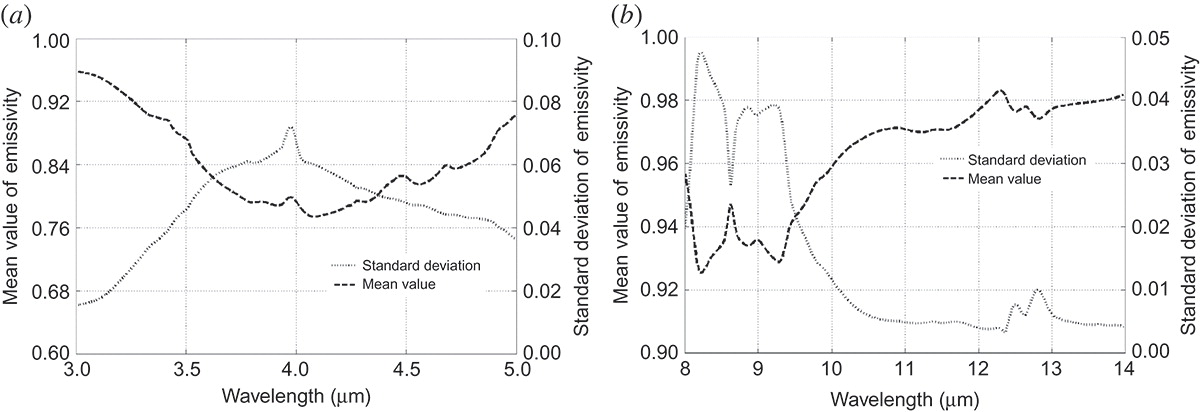
\includegraphics[width=0.9\textwidth]{emi_soil.jpeg}
  \caption{Emissivity spectra for soils in the ASTER spectral emissivity database. (a) 3 - 5 $\mu$m. (b) 8 - 14 $\mu$m. \parencite{Reference303}.}
  \label{fig:emi_soil}
  
  \centering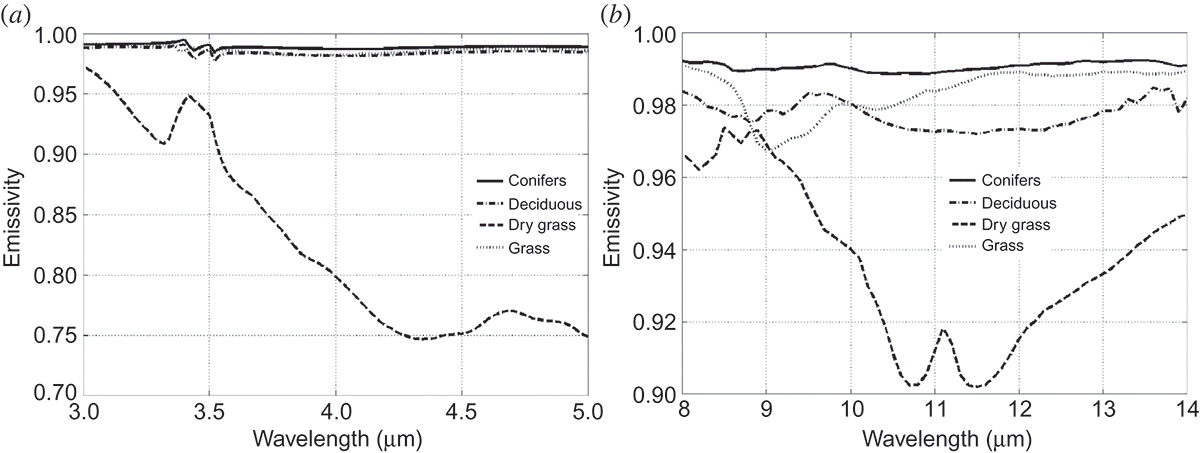
\includegraphics[width=0.9\textwidth]{emi_vegetation.jpeg}
  \caption{Emissivity spectra for four types of vegetation in the ASTER spectral emissivity database. (a) 3 - 5 $\mu$m. (b) 8 - 14 $\mu$m. \parencite{Reference303}.}
  \label{fig:emi_vegetation}
  
  \centering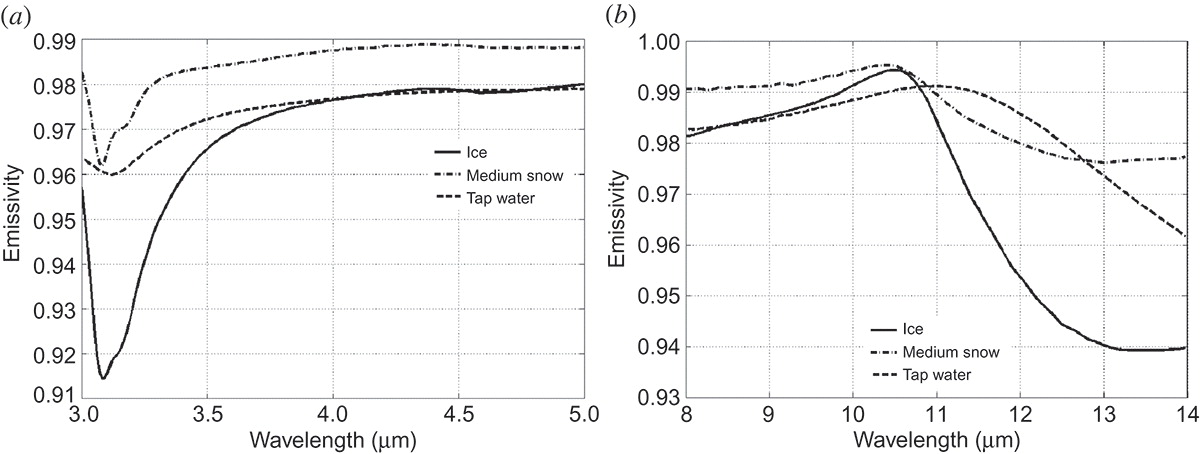
\includegraphics[width=0.9\textwidth]{emi_water.jpeg}
  \caption{Emissivity spectra for water, ice and snow in the ASTER spectral emissivity database. (a) 3 - 5 $\mu$m. (b) 8 - 14 $\mu$m. \parencite{Reference303}.}
  \label{fig:emi_water}
\end{figure}

\noindent Denote the product $\varepsilon(k) L_{bb}(k, T) = L_{surf}^*(k, T)$ as the ''effective'' or ''radiative'' surface radiance, we can get:
\begin{equation}
\label{eq305}
L_{surf}^*(k, T) = \frac{L(k) - L_p(k)}{\tau (k)} - (1 - \varepsilon (k)) \frac{F(k)}{\pi}
\end{equation}

\noindent Given in both MIR and TIR band the emissivity is close to 1, so the term $1 - \varepsilon (k)$ will be such a small term that the thermal downwelling flux term $F(k)$ will have only a small influence. Finally, all the terms $L_p(k)$, $F(k)$ and $\tau (k)$ will be calculated by MODTRAN (MODerate resolution atmospheric TRANsmission) as a function of atmospheric water vapor volumn $W(e)$, $W$ for short, which acts as a function of elevation $e$, for MIR and TIR band of TET-1 imagery respectively.\\

\noindent Finally, the surface radiance of both the black body and natural materials can be calculated from Equation \eqref{eq305}. The atmospheric correction for the night-time TET-1 scenes are done.\\

\noindent With the help of Planck's function and its inversion, surface temperature for the MIR and TIR band of TET-1 imagery can be derived. Using the dual-channel method proposed by Matson and Dozier (1981), the final HTE monitoring products including effective target temperature $T_t$, effective target pixel fraction and Fire Radiative Power (FRP) can be obtained.\\

%----------------------------------------------------------------------------------------
%	SECTION 3
%----------------------------------------------------------------------------------------

\section{Outcomes of the MITIP}
The outcomes of MITIP can be classified into two parts: one part is the result of atmospheric correction and another the HTE monitoring product.\\

\noindent The result of atmospheric correction is the surface radiance in MIR and TIR band respectively. There are two types of surface radiance files:
\begin{itemize}
\item The ''blackbody'' surface radiance with $\varepsilon_{MIR} = \varepsilon_{TIR} = 1$;
\item The ''graybody'' surface radiance accounting for the input emissivity map $\varepsilon_{TIR}$ and assuming $\varepsilon_{MIR} = \varepsilon_{TIR}$;
\end{itemize}

\noindent The HTE monitoring product is one GeoTIFF file which consists of six bands:
\begin{itemize}
\item Band 1: surface temperature map in MIR band, $T_{MIR}$ [K];
\item Band 2: surface temperature map in TIR band, $T_{TIR}$ [K];
\item Band 3: fire probability map indicating which pixel might contain high-temperature events. For non-fire pixels, the pixel value are 0; for each detected fire pixel, the fire probability is assigned between 0.8 to 1.0;
\item Band 4: effective target temperature map [K]. For every detected fire pixel, the effective target temperature $T_t$ is calculated.  Otherwise the pixel value is set to 0;
\item Band 5: effective target pixel fraction map. The same as the effective target temperature map, for each detected fire pixel, the effective target pixel fraction $p$ is calculated. For the rest, their pixel values are set to 0;
\item Band 6: fire radiative power (FRP) [MW] map;
\end{itemize}

\noindent If, for one scene, no fire pixels are detected, the output files of HTE monitoring contains only the MIR and TIR band surface temperature maps.\\
\chapter{Validation and improvement of the MITIP}

\label{Chapter4}

%description
%----------------------------------------------------------------------------------------
In this chapter, to see whether the temperature products derived from MITIP is reliable or not, its results are compared with MODIS temperature products, namely MODIS Sea Surface Temperature (SST) and MODIS Land Surface Temperature (LST). Two test sites, Etna and Libya, are selected to do the comparisons because their imageries mainly covered by sea (Etna) and homogeneous landscape (Libya) respectively.\\

%----------------------------------------------------------------------------------------
%	SECTION 1
%----------------------------------------------------------------------------------------

\section{Analysis of normal temperature environments}

%-----------------------------------
%	SUBSECTION 1
%-----------------------------------

\subsection{Data preparation and processing}
The MODIS temperature products are downloaded from NASA's website. In order to do the comparison more effectively, the downloaded data will be pre-processed using the same steps as the inputed data described in Chapter 3.\\

\noindent After pre-processing, here the MODIS SST is used as an example, the MODIS SST product is showed in Figure \ref{fig:SST}. The differences of the surface temperature between MODIS temperature products and MITIP surface temperature maps in MIR and TIR band are computed through the whole imageries respectively. Then, for each scene, several sub-areas which are cloud-free and homogeneous inside are selected as test areas for the comparison as Figure \ref{fig:selectedArea} shows. Outliers caused by NoDataValue of MODIS temperature products and cloud e.t.c are filtered out and the mean of the temperature differences $\Delta T_i$ of each sub-area $i$ is calculated.\\

\noindent Finally, the mean value $\overline{\Delta T}$ over all sub-areas within one scene are computed to denote the temperature difference between MODIS temperature products and MITIP results for that scene.\\
\begin{equation}
\label{eq1}
\overline{\Delta T} =\frac{\sum_{i=1}^m \Delta T_i}{m}
\end{equation}
with $m$ is the total number of the sub-areas. Here $m = 4$.

\begin{figure}[!htbp]
\centering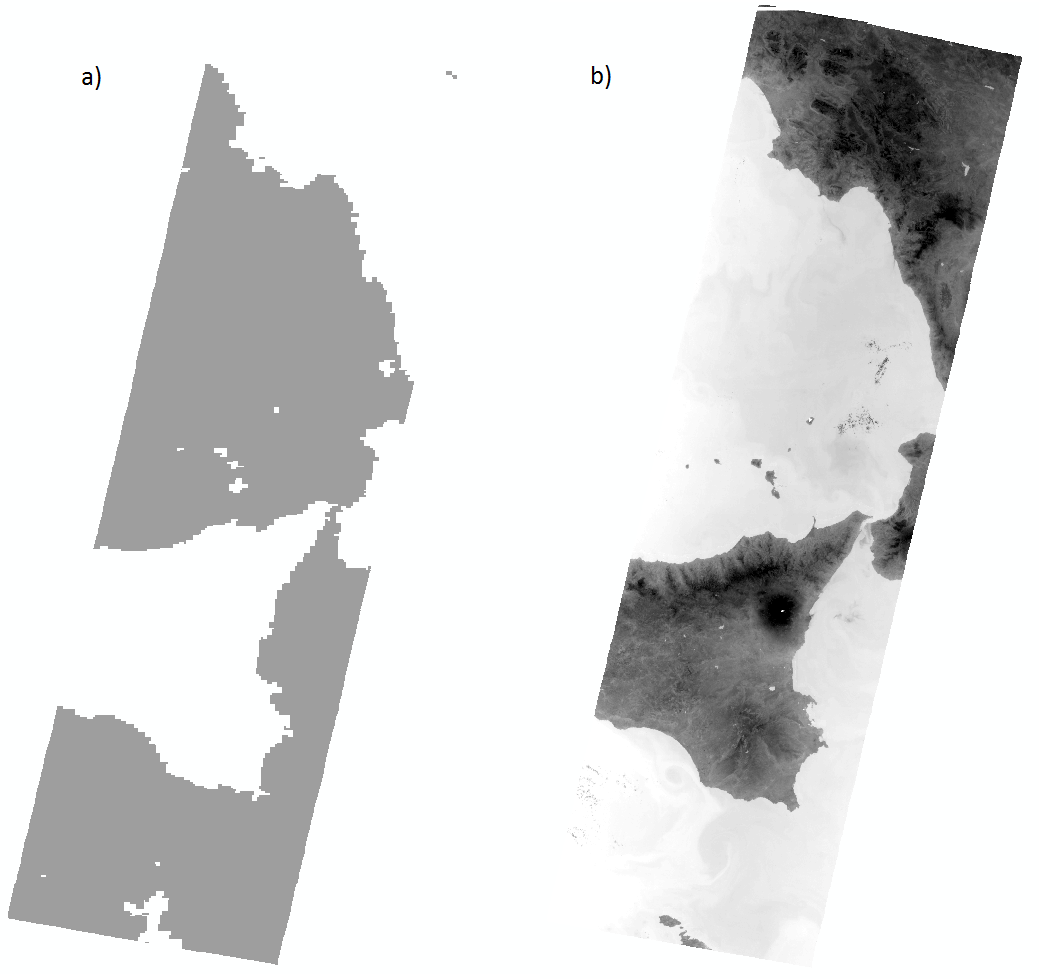
\includegraphics[width=0.6\textwidth]{SST.png}
\caption{a) MODIS SST. b) MITIP temperature product: surface temperature map in MIR band}
\label{fig:SST}
\end {figure}

\begin{figure}[!htbp]
\centering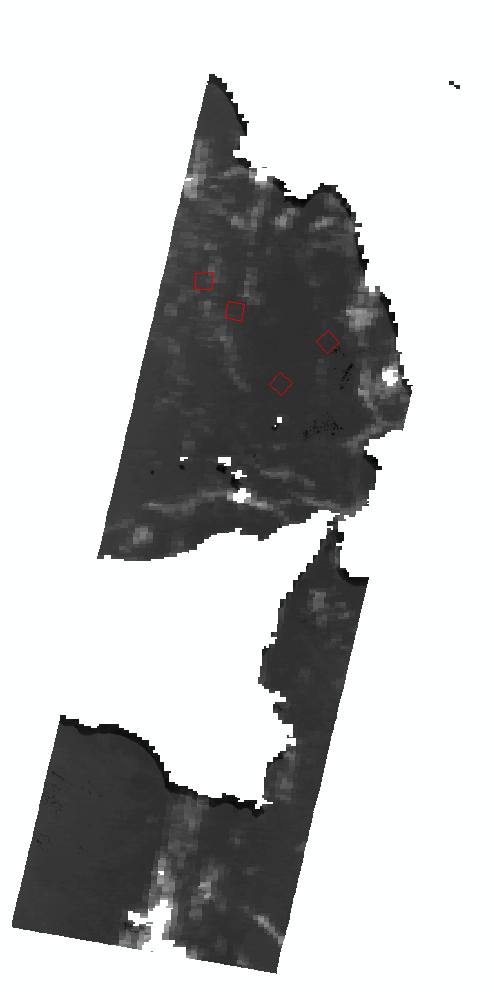
\includegraphics[width=0.4\textwidth]{differences.png}
\caption{Difference map between MODIS SST and MITIP surface temperature in MIR band}
\label{fig:Diff}
\end{figure}

\begin{figure}[!htbp]
\centering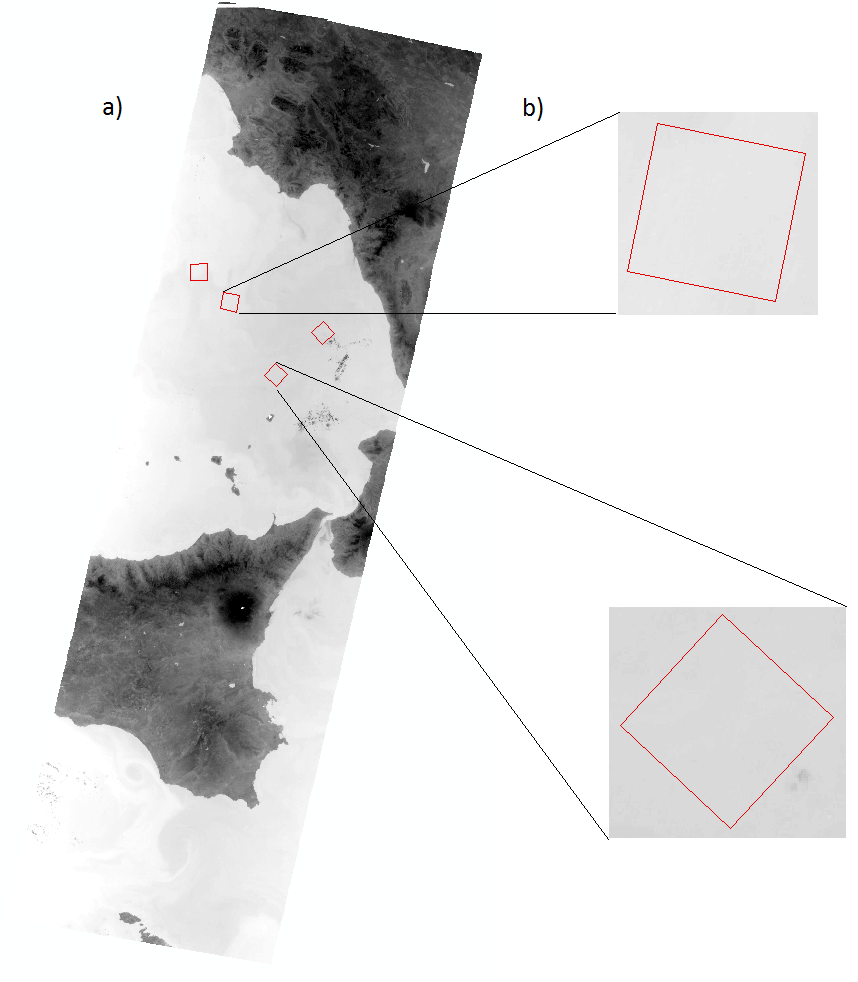
\includegraphics[width=0.6\textwidth]{selectedArea.png}
\caption{a) Selected sub-areas distribution over MITIP surface temperature in MIR band. b) Zoomed-in pictures of two sub-areas}
\label{fig:selectedArea}
\end{figure}

%-----------------------------------
%	SUBSECTION 2
%-----------------------------------

\subsection{Results comparison with MODIS SST and calibration}
Before doing the comparison between MODIS SST and MITIP surface temperature products, one problem needs to be solved is that the choice of emissivity map. The emissivity map derived from ASTER Global Emissivity Database is consisted of 5 bands and there are two bands, namely band 11 with wavelength 8.6 $\mu$m and band 12 with wavelength 9.1 $\mu$m fall in TET-1 imagery's TIR band with spectral range 8.5 $\mu$m to 9.3 $\mu$m \parencite{Reference306}. So there comes a problem that which band of the emissivity maps should be used. This problem will be considered under different circumstances.\\

\noindent Since the emissivities of water body in these two bands are very close, 0.984  and 0.985 respectively, the effects of the different emissivities can be neglected when the results from MITIP are compared with MODIS SST as shown Figure \ref{fig:tem_diff_emi1}.\\

\begin{figure}[!htbp]
\centering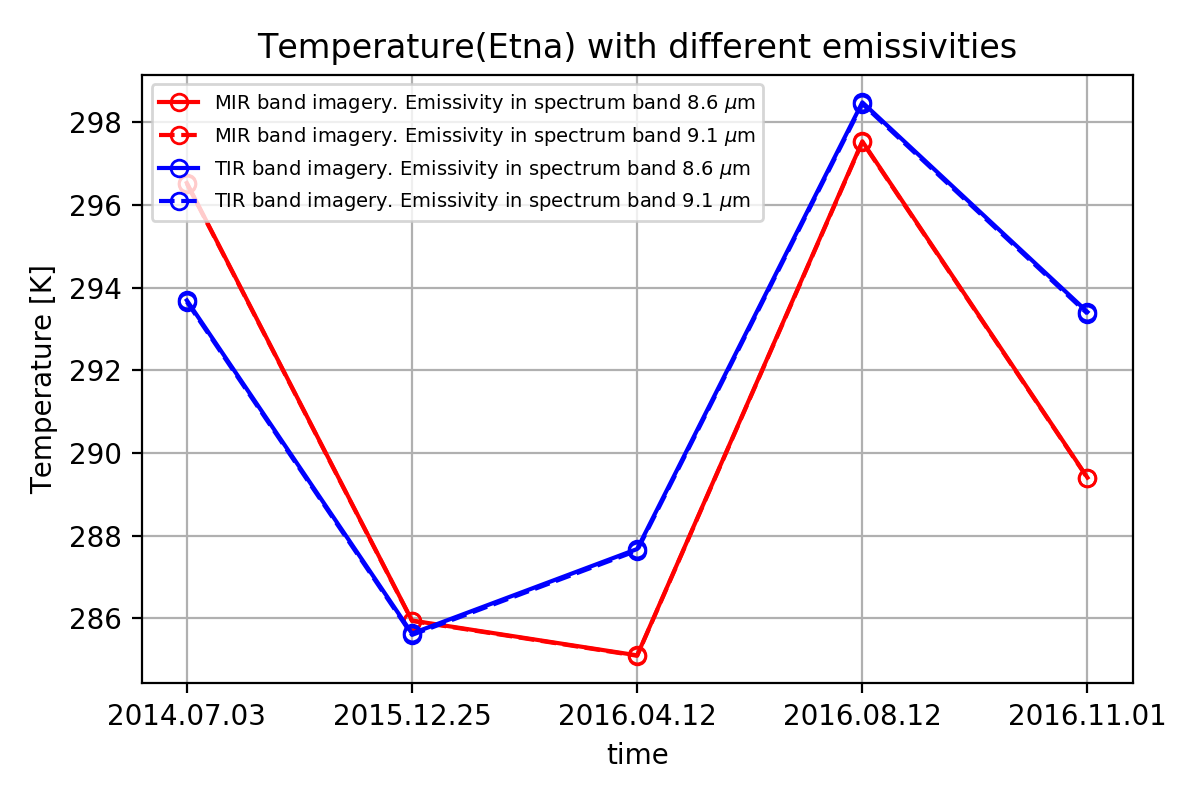
\includegraphics[width=0.8\textwidth]{diff_emi1.png}
\caption{Mean temperature of all sub-areas in Etna scenes with different emissivities}
\label{fig:tem_diff_emi1}
\end{figure}

\begin{figure}[!htbp]
\centering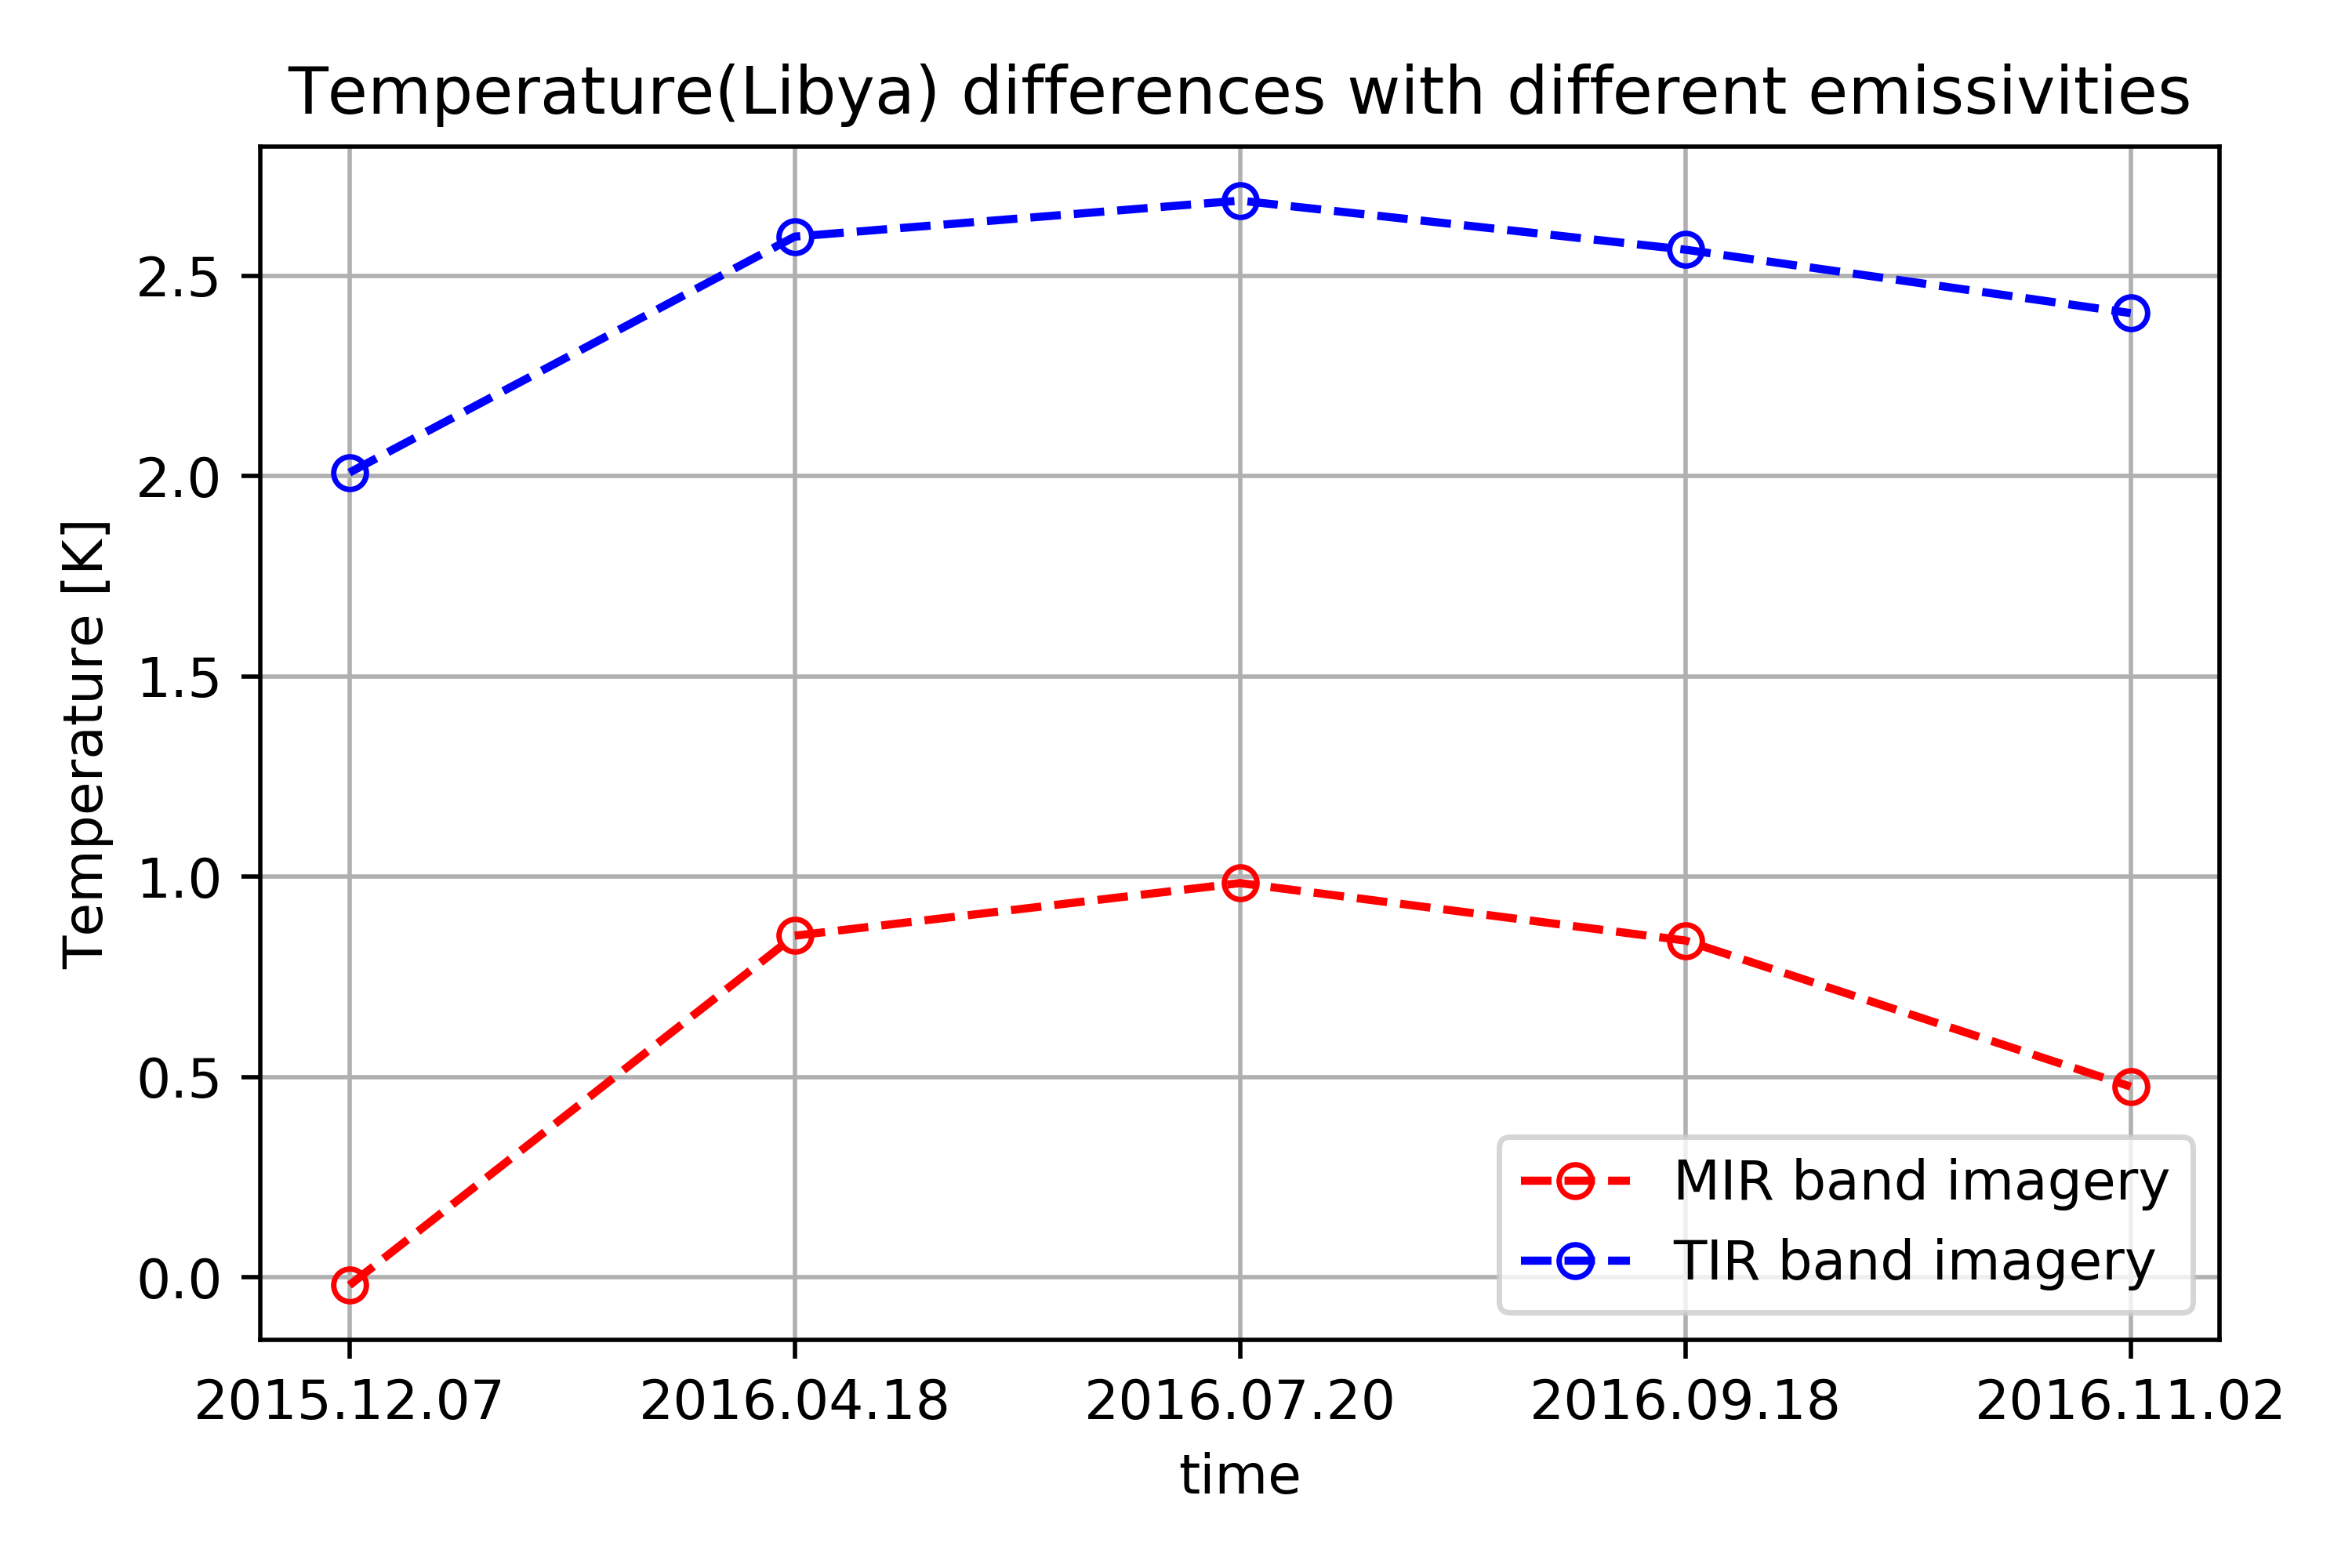
\includegraphics[width=0.8\textwidth]{diff_emi2.png}
\caption{Differences of temperatures resulted from different emissivities(Etna)}
\label{fig:tem_diff_emi2}
\end{figure}

\noindent From Figure \ref{fig:tem_diff_emi2} we can see that the temperature differences resulted from different emissivities in MIR band imagries are within the range (0.010K, 0.018K). The temperature differences resulted from different emissivities in TIR band imagries are within the range (0.032K, 0.040K). Both of them are so small that can be neglected in the context of the area of interest (AOI) is water body. Here the emissivity map in band 8.6 $\mu$m is used.\\

\noindent Firstly, the surface temperature maps from MITIP are compare with MODIS SST according to the steps states in Section 4.1. The Figure \ref{fig:tem_com} shows that the surface temperatures derived by MITIP are lower than the MODIS SST on both the MIR band and TIR band. To adjust these differences, TOA radiances, which are the pixel values of the original TET-1 imageries, need to be calibrated.\\

\begin{figure}[!htbp]
\centering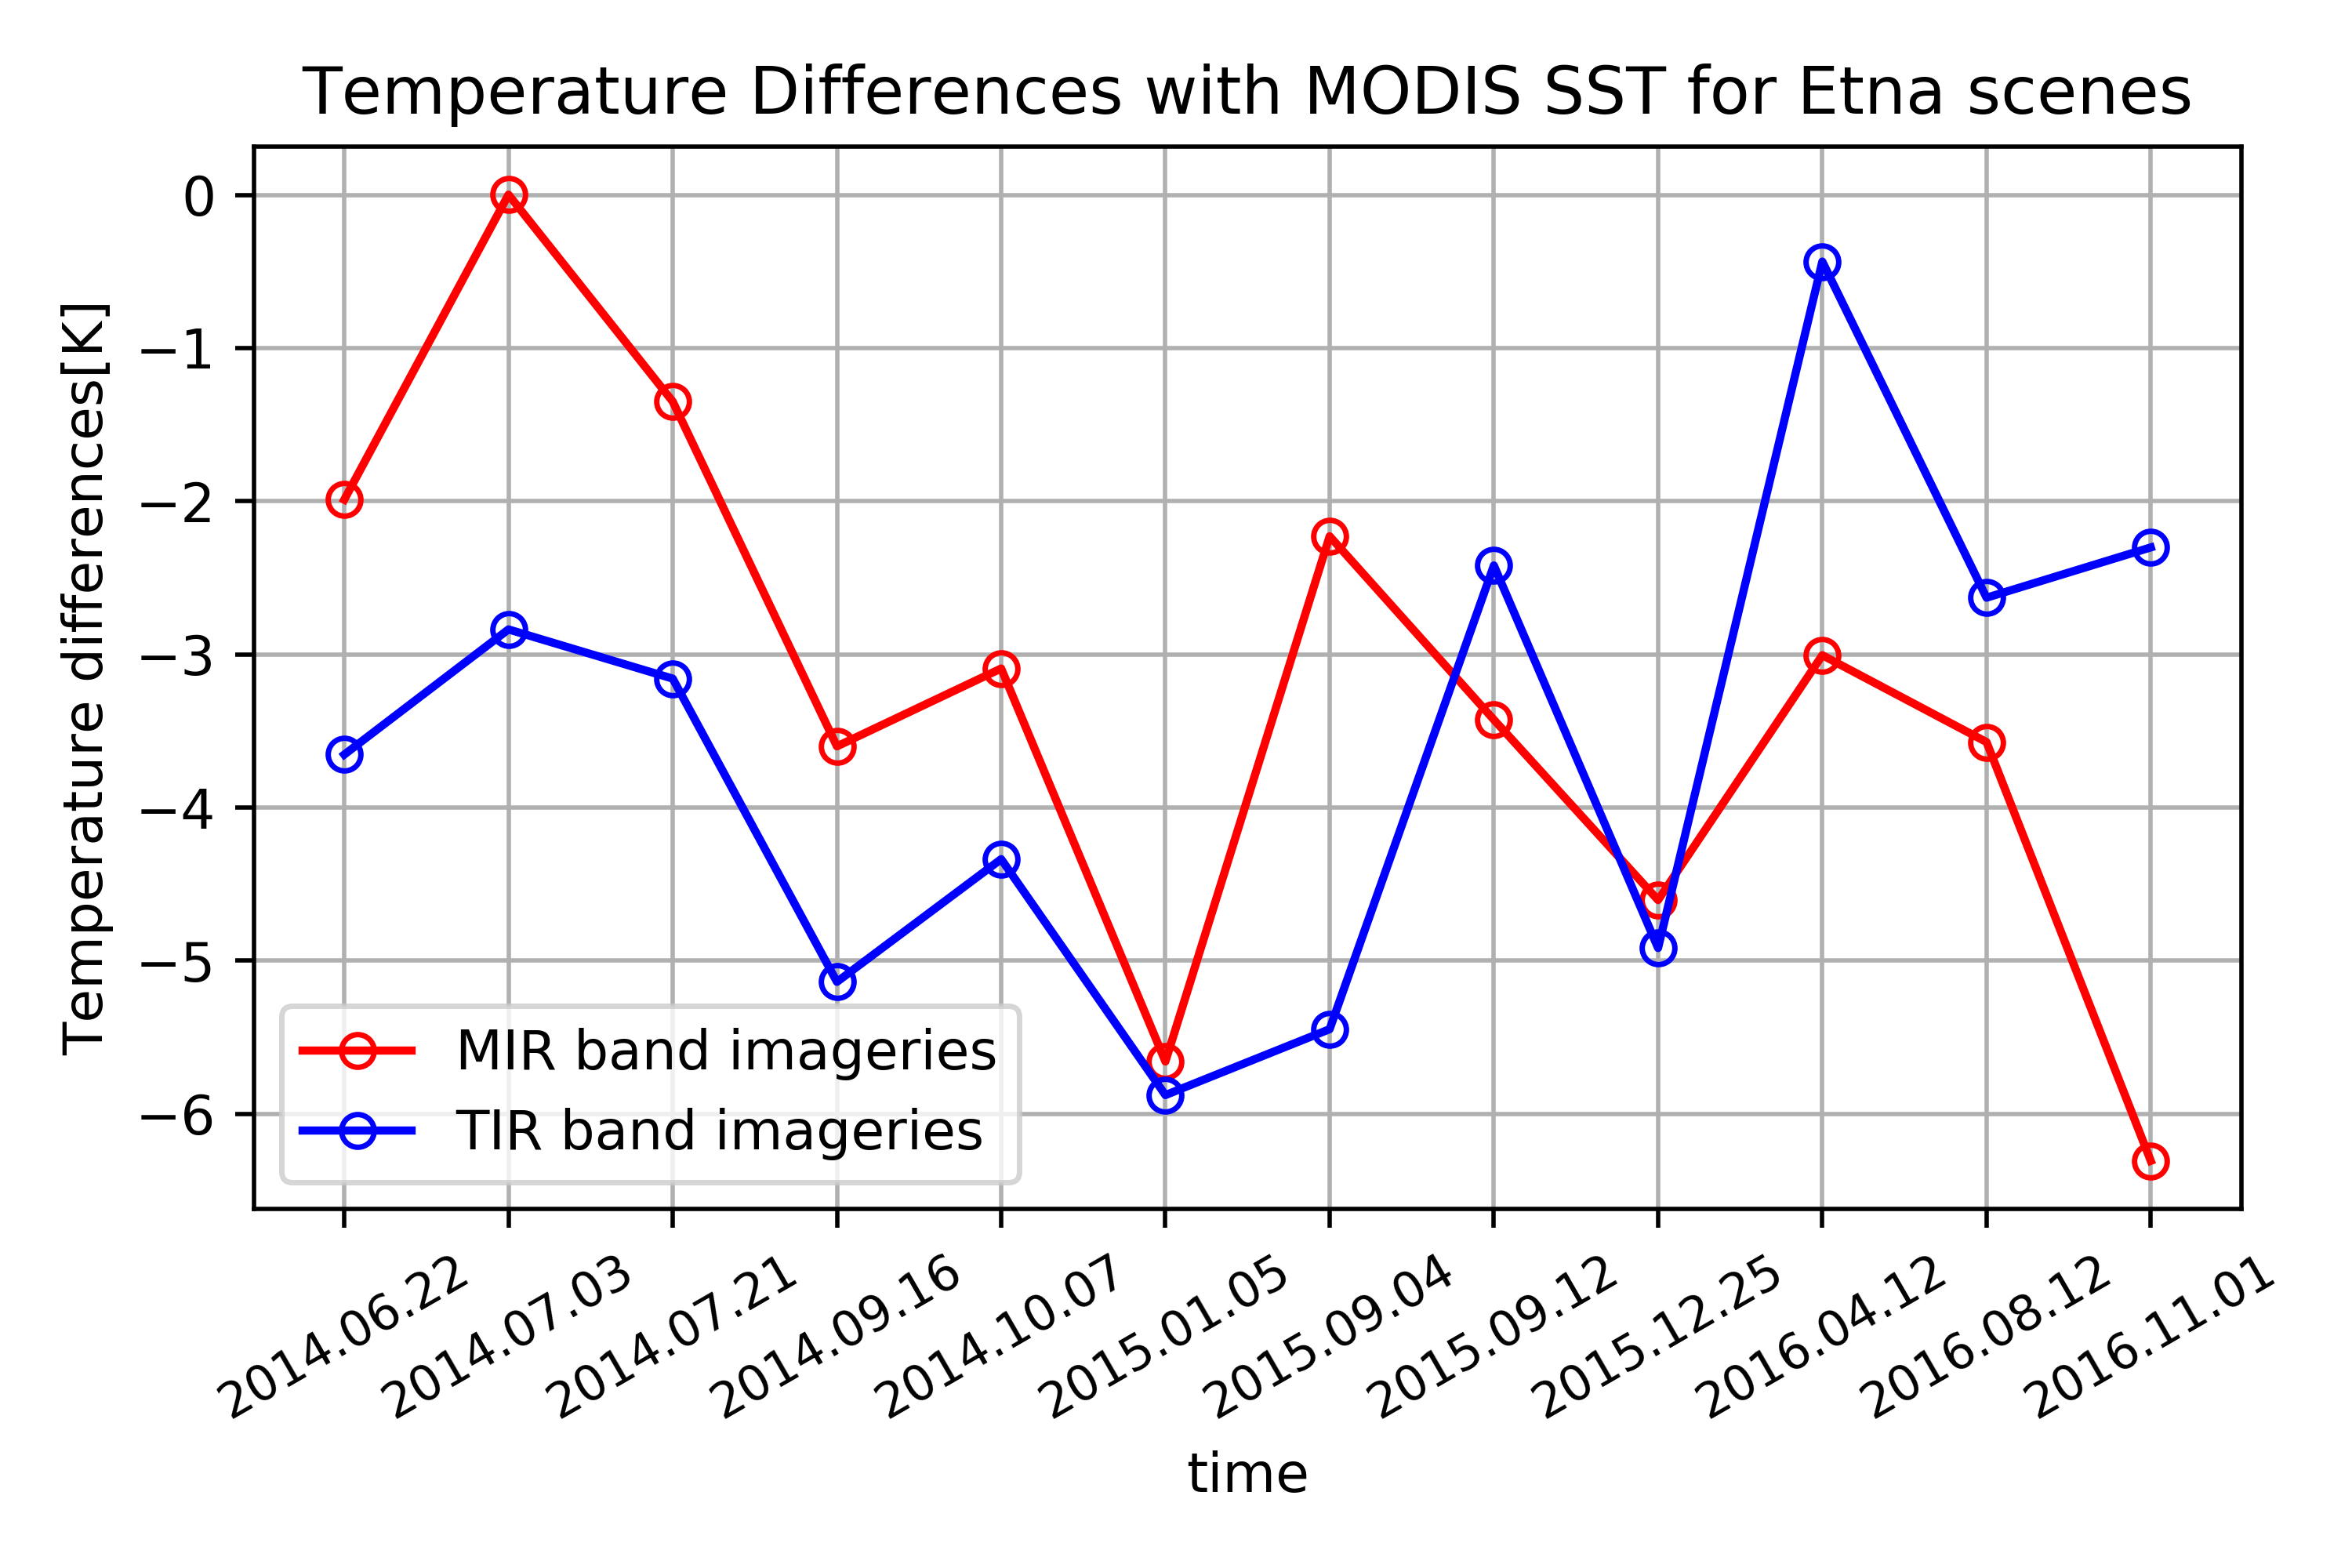
\includegraphics[width = 0.8\textwidth]{tem_com.png}
\caption{Temperature differences between the temperature maps from MITIP and MODIS SST for Etna scenes}
\label{fig:tem_com}
\end{figure}

\noindent As a result, the MITIP method adds two input keywords \emph{sc1} and \emph{sc2}, which stand for scale factor for the TET-1 MIR and TIR band imagries respectively, to calibrate the TOA radiances. Since the temperatures derived from MITIP are lower than the MODIS SST, the TOA radiances of the TET-1 imagriy should be increased. As a result, five scale factors, 1.00 which means original TOA radiances, 1.05 which means increasing the TOA radiances by 5\%, 1.10, 1.15 and 1.20, are selected to calibrate the TET-1 MIR and TIR band respectively.\\

\noindent In order to see detailedly how the scale factor will affect the pixel values of the results of MITIP, histograms of sub-areas of TET-1 MIR band temperature map are investigated and compared with the histograms of the same areas of MODIS SST. The histograms of each sub-area with different scale factors are showed in Figure \ref{fig:hist_rect_all}. Here we use the Etna scene of the date 2014.06.22, which is the first scene we have for the Etna.\\

\begin{figure}[!htbp]
\centering
\subfigure[Sub-area 1 with scale factor 1.00]{
\label{fig:hist_rect1_1}
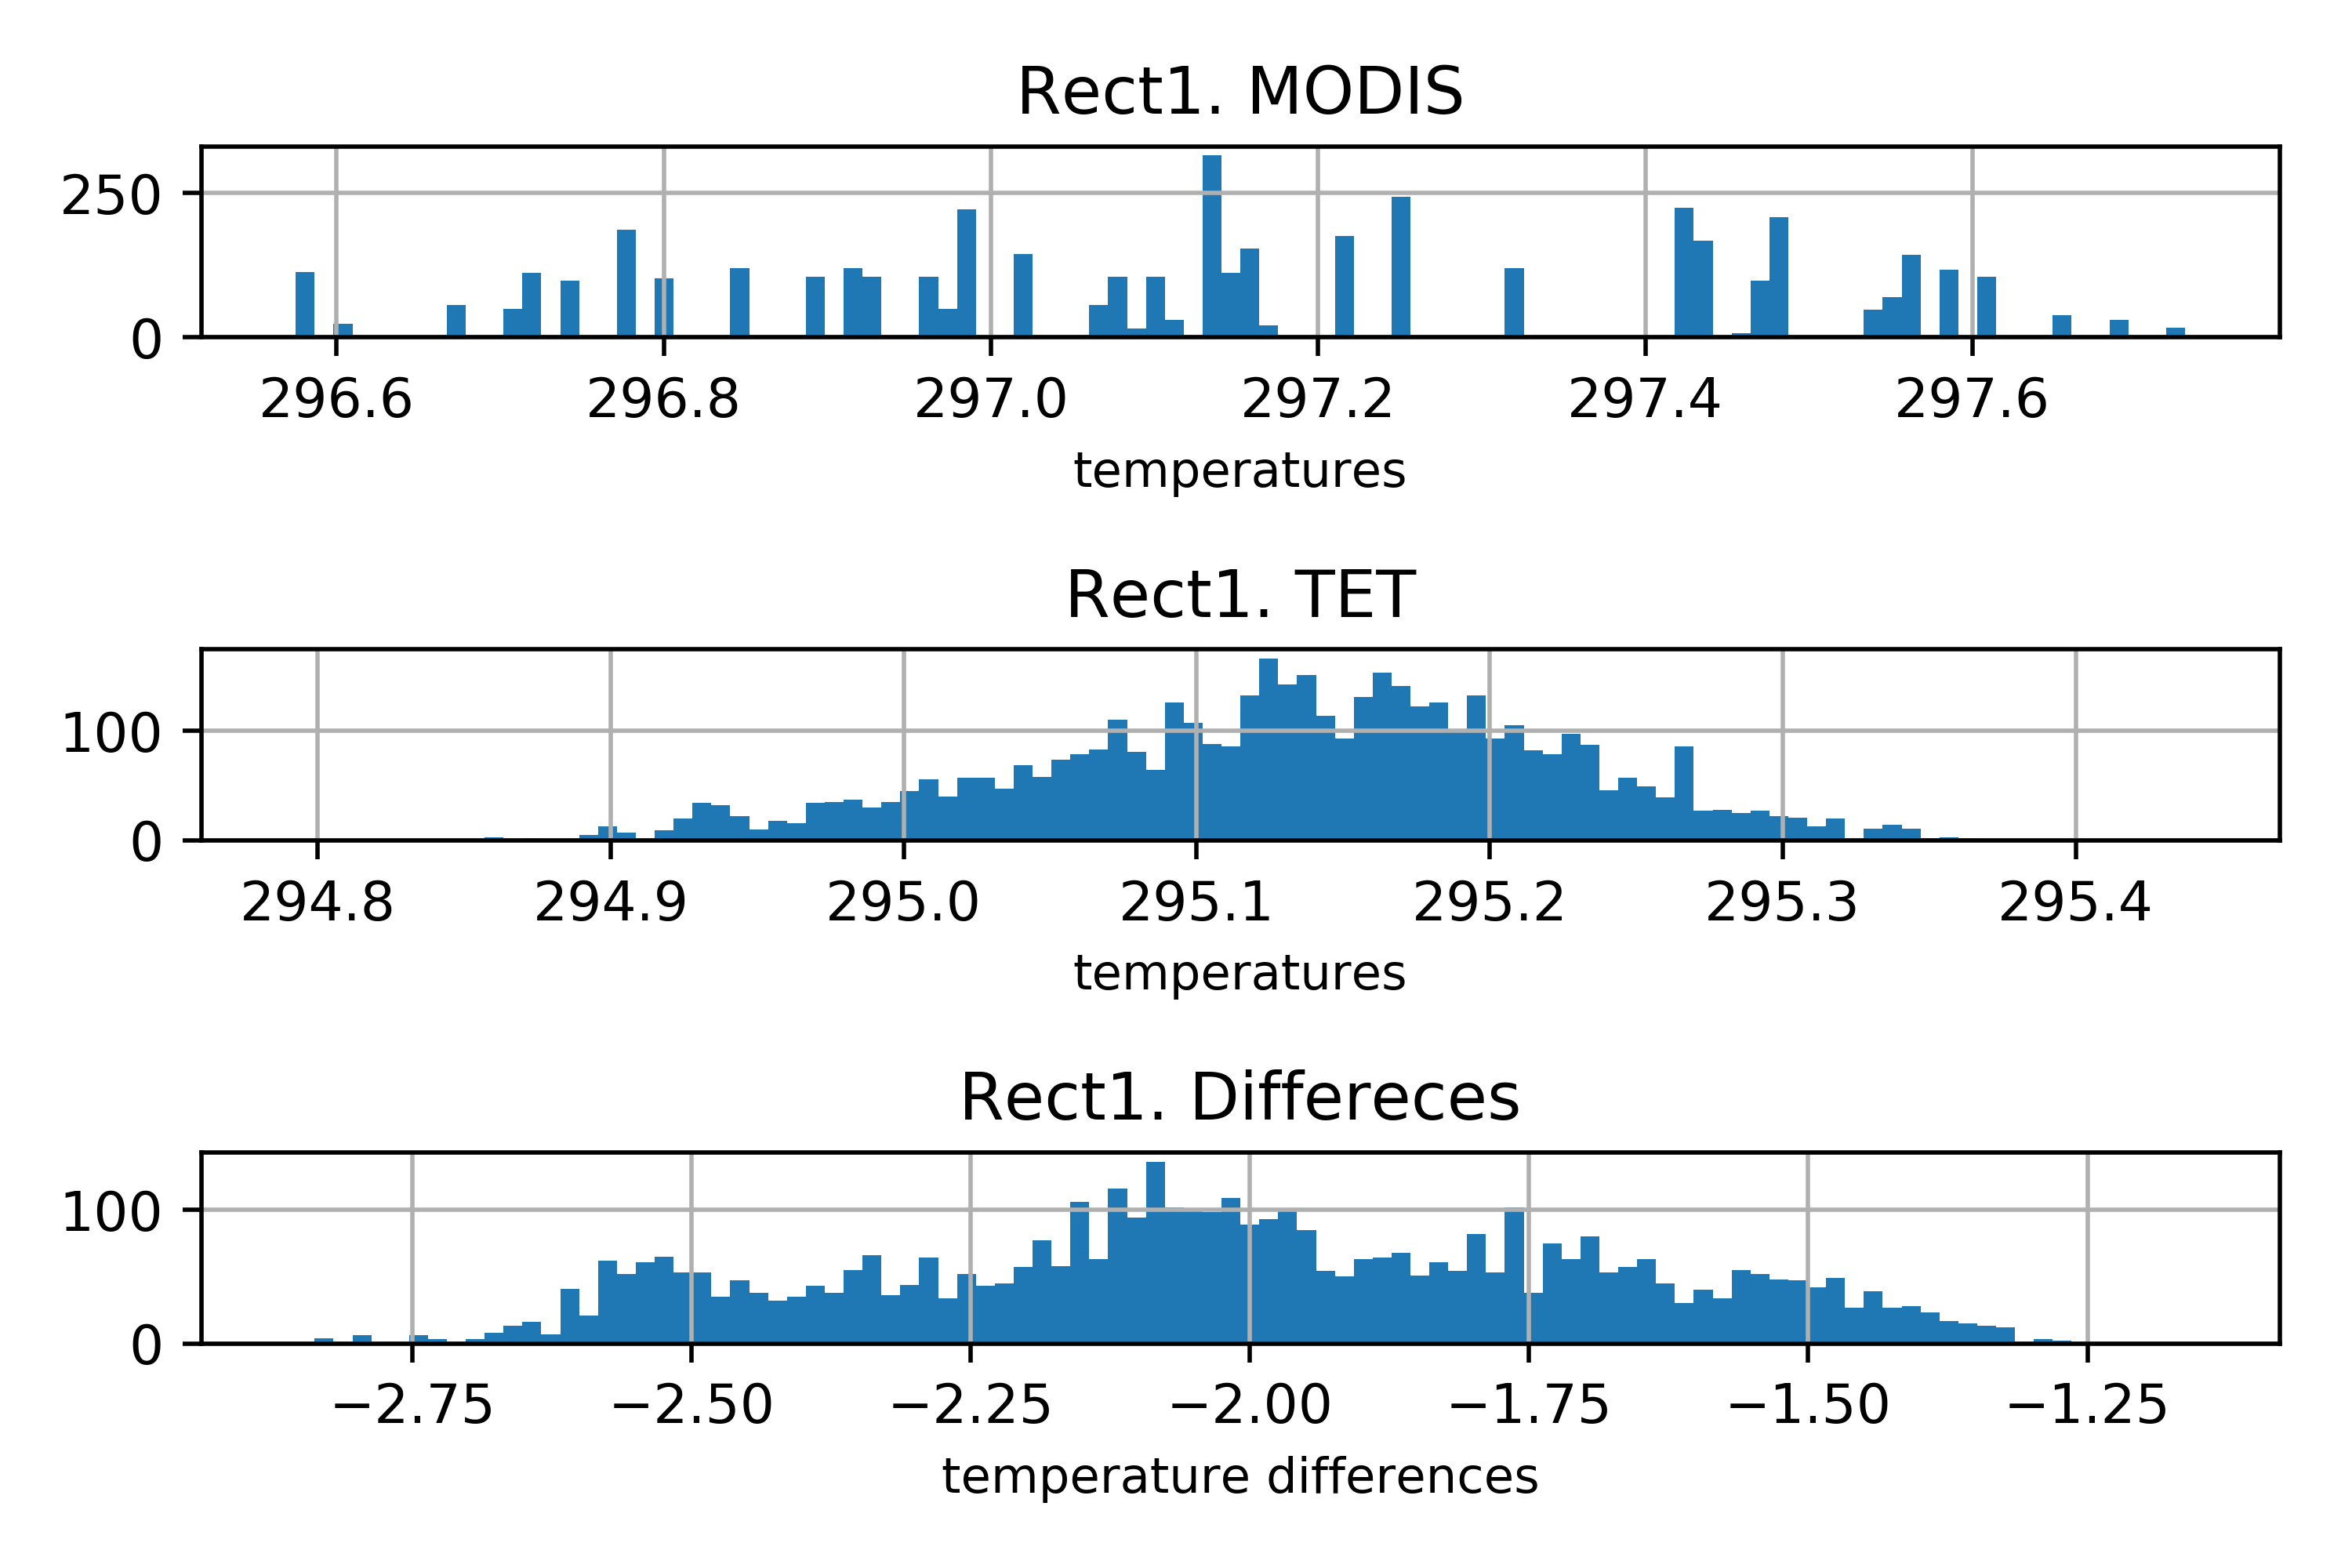
\includegraphics[width = 0.48\linewidth]{rect1_sc100.png}}
\vspace{0.1in}
\subfigure[Sub-area 1 with scale factor 1.10]{
\label{fig:hist_rect1_2}
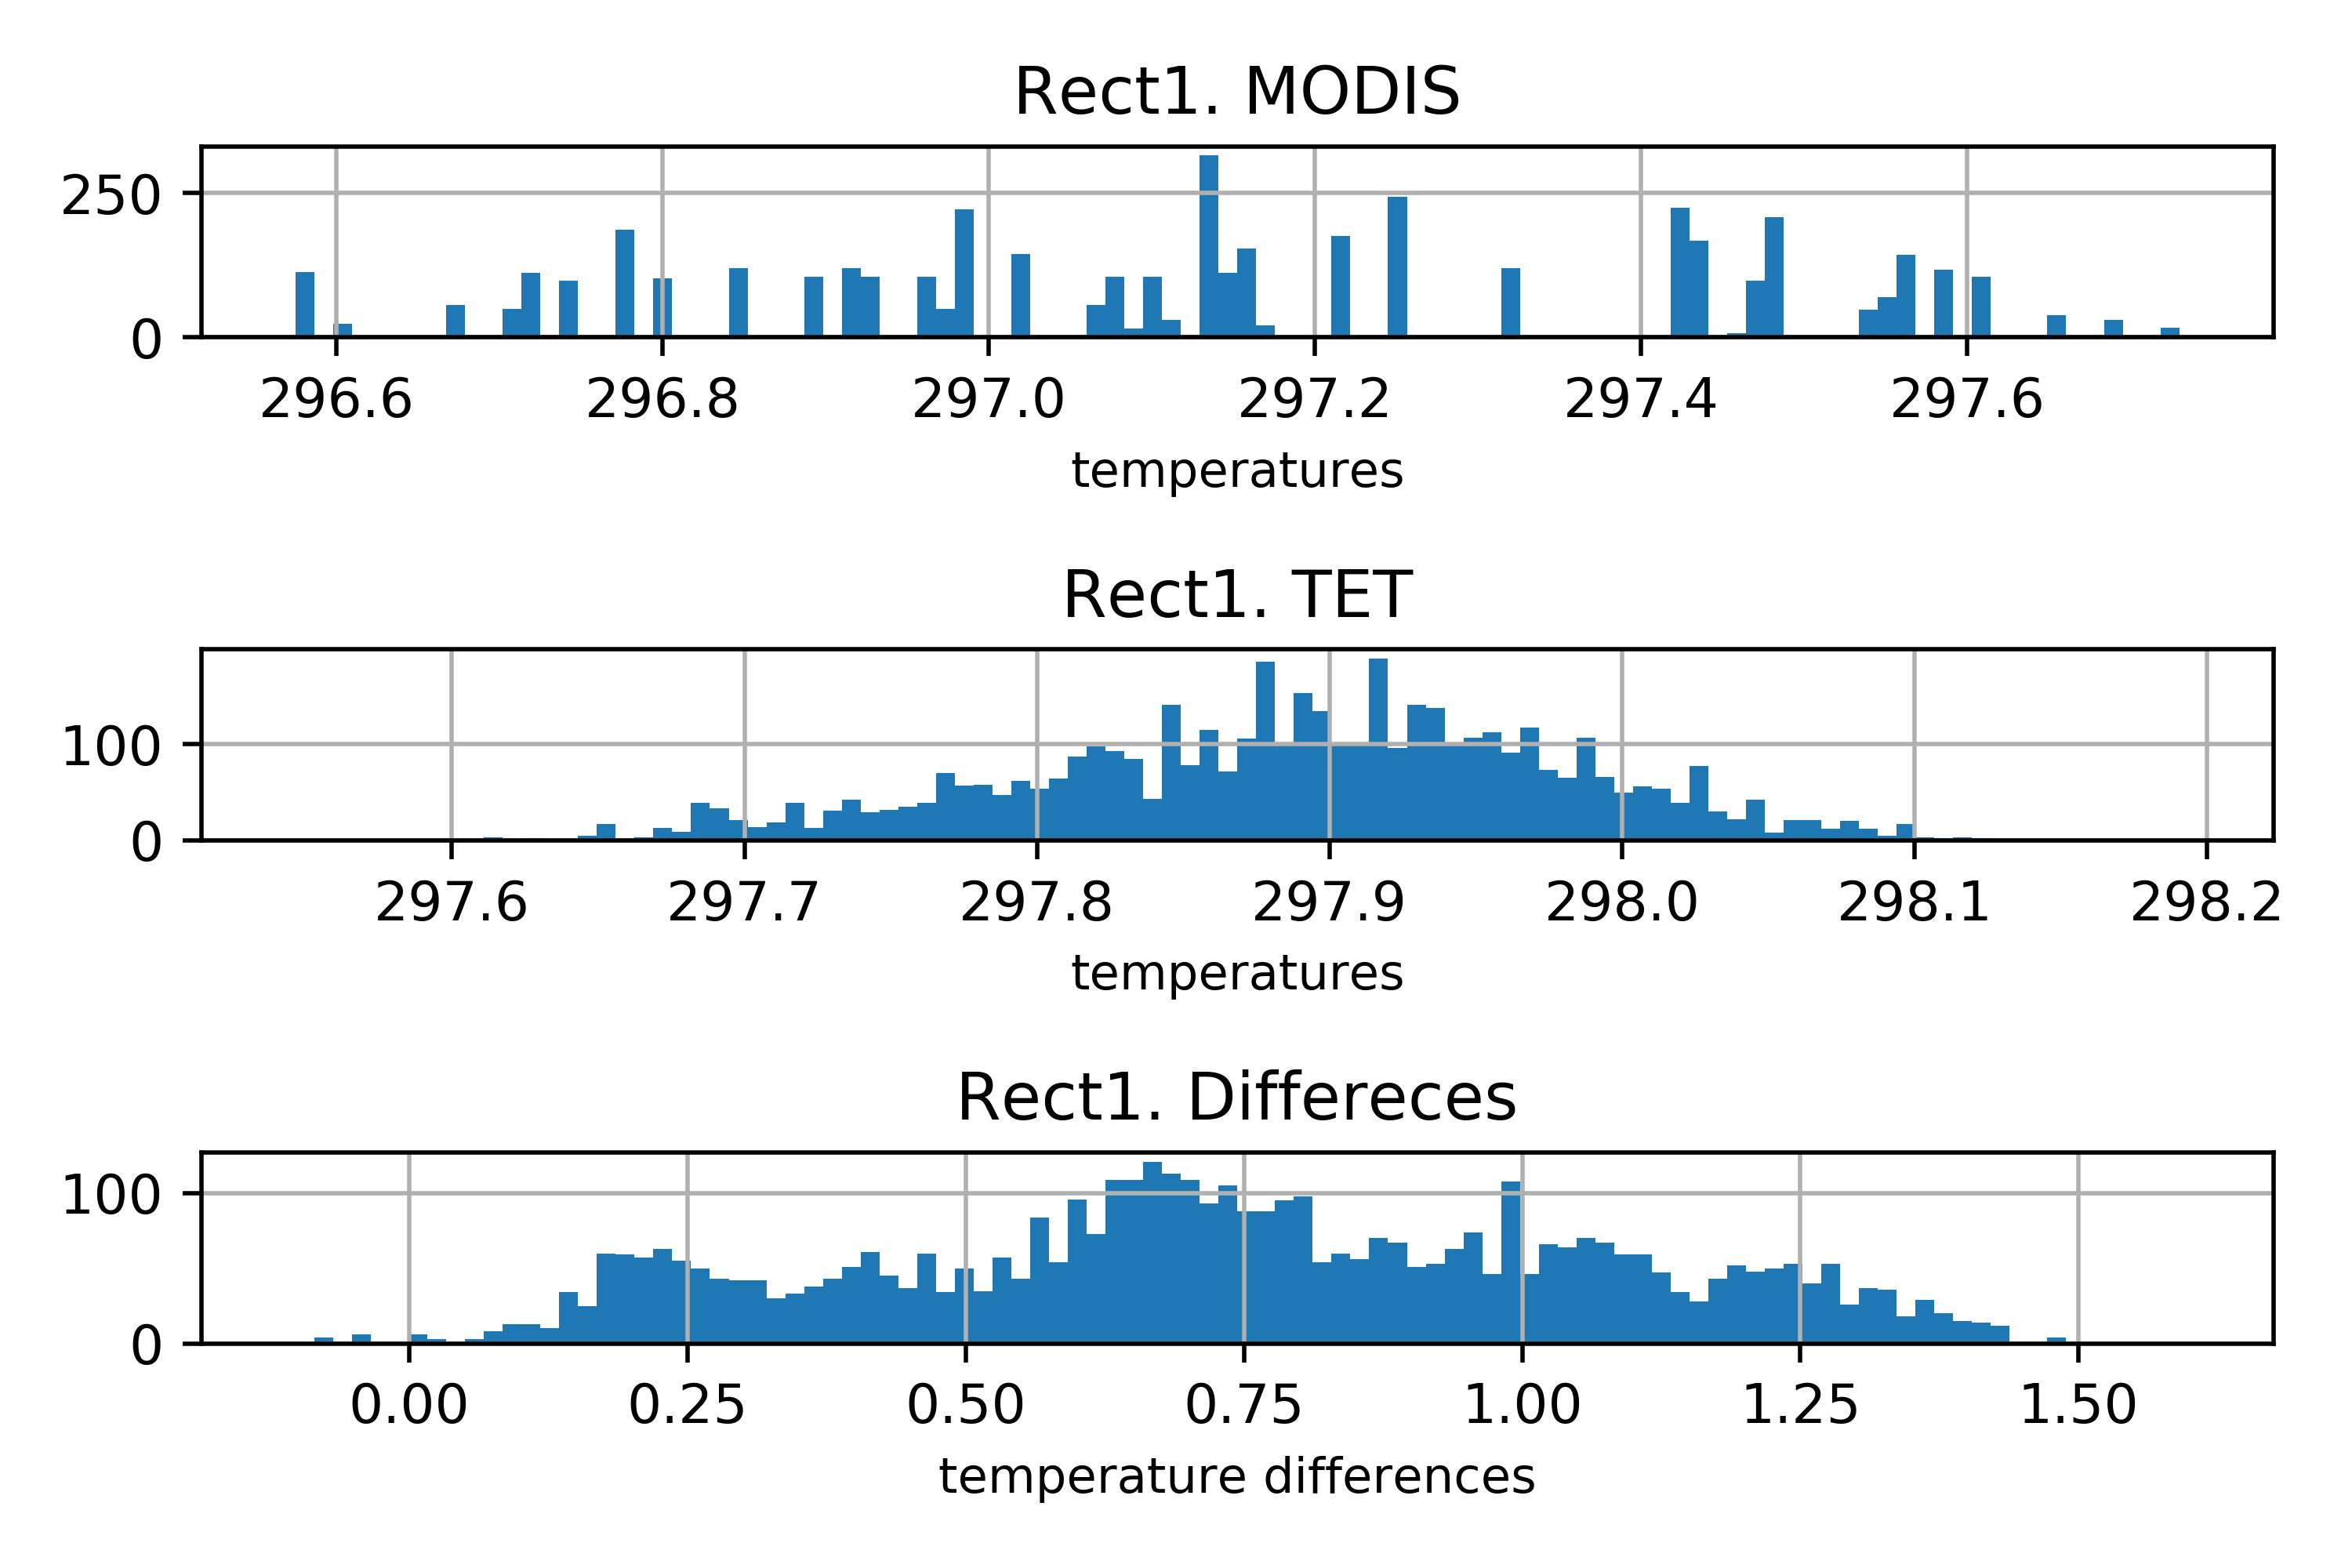
\includegraphics[width = 0.48\linewidth]{rect1_sc110.png}}

\hspace{0.5in}

\subfigure[Sub-area 2 with cale factor 1.00]{
\label{fig:hist_rect2_1}
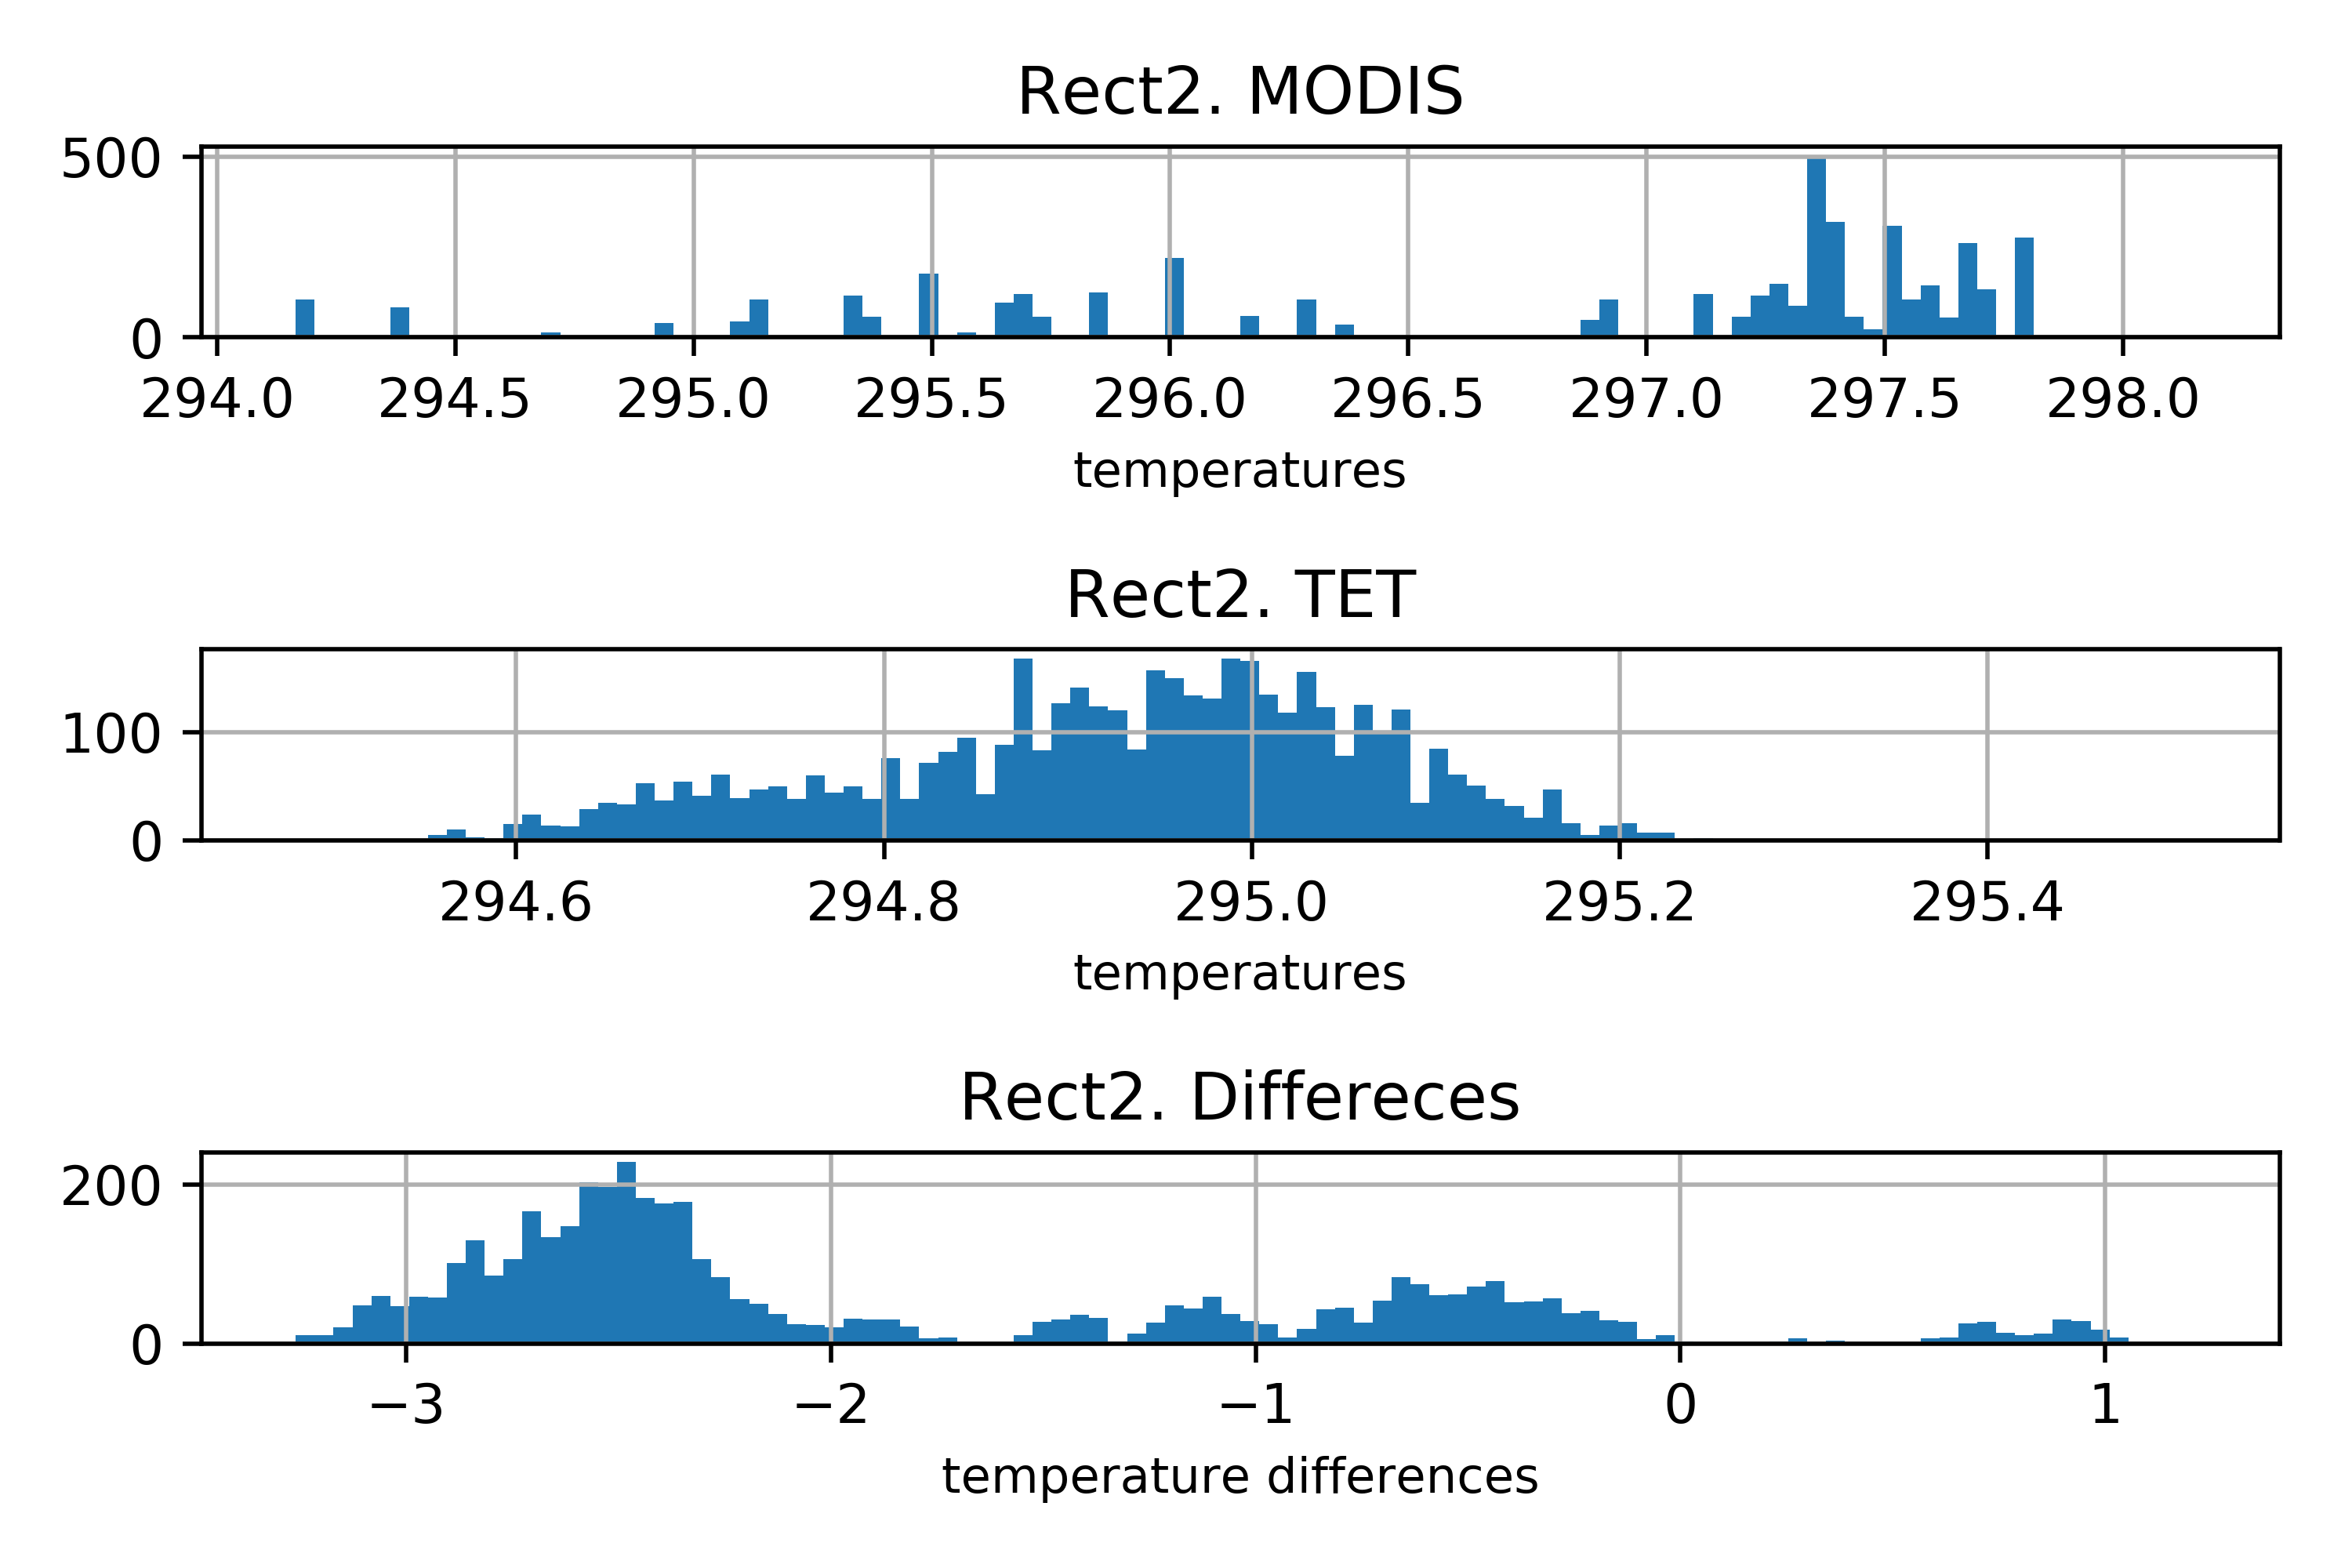
\includegraphics[width = 0.48\linewidth]{rect2_sc100.png}}
\vspace{0.1in}
\subfigure[Sub-area 2 with cale factor 1.10]{
\label{fig:hist_rect2_2}
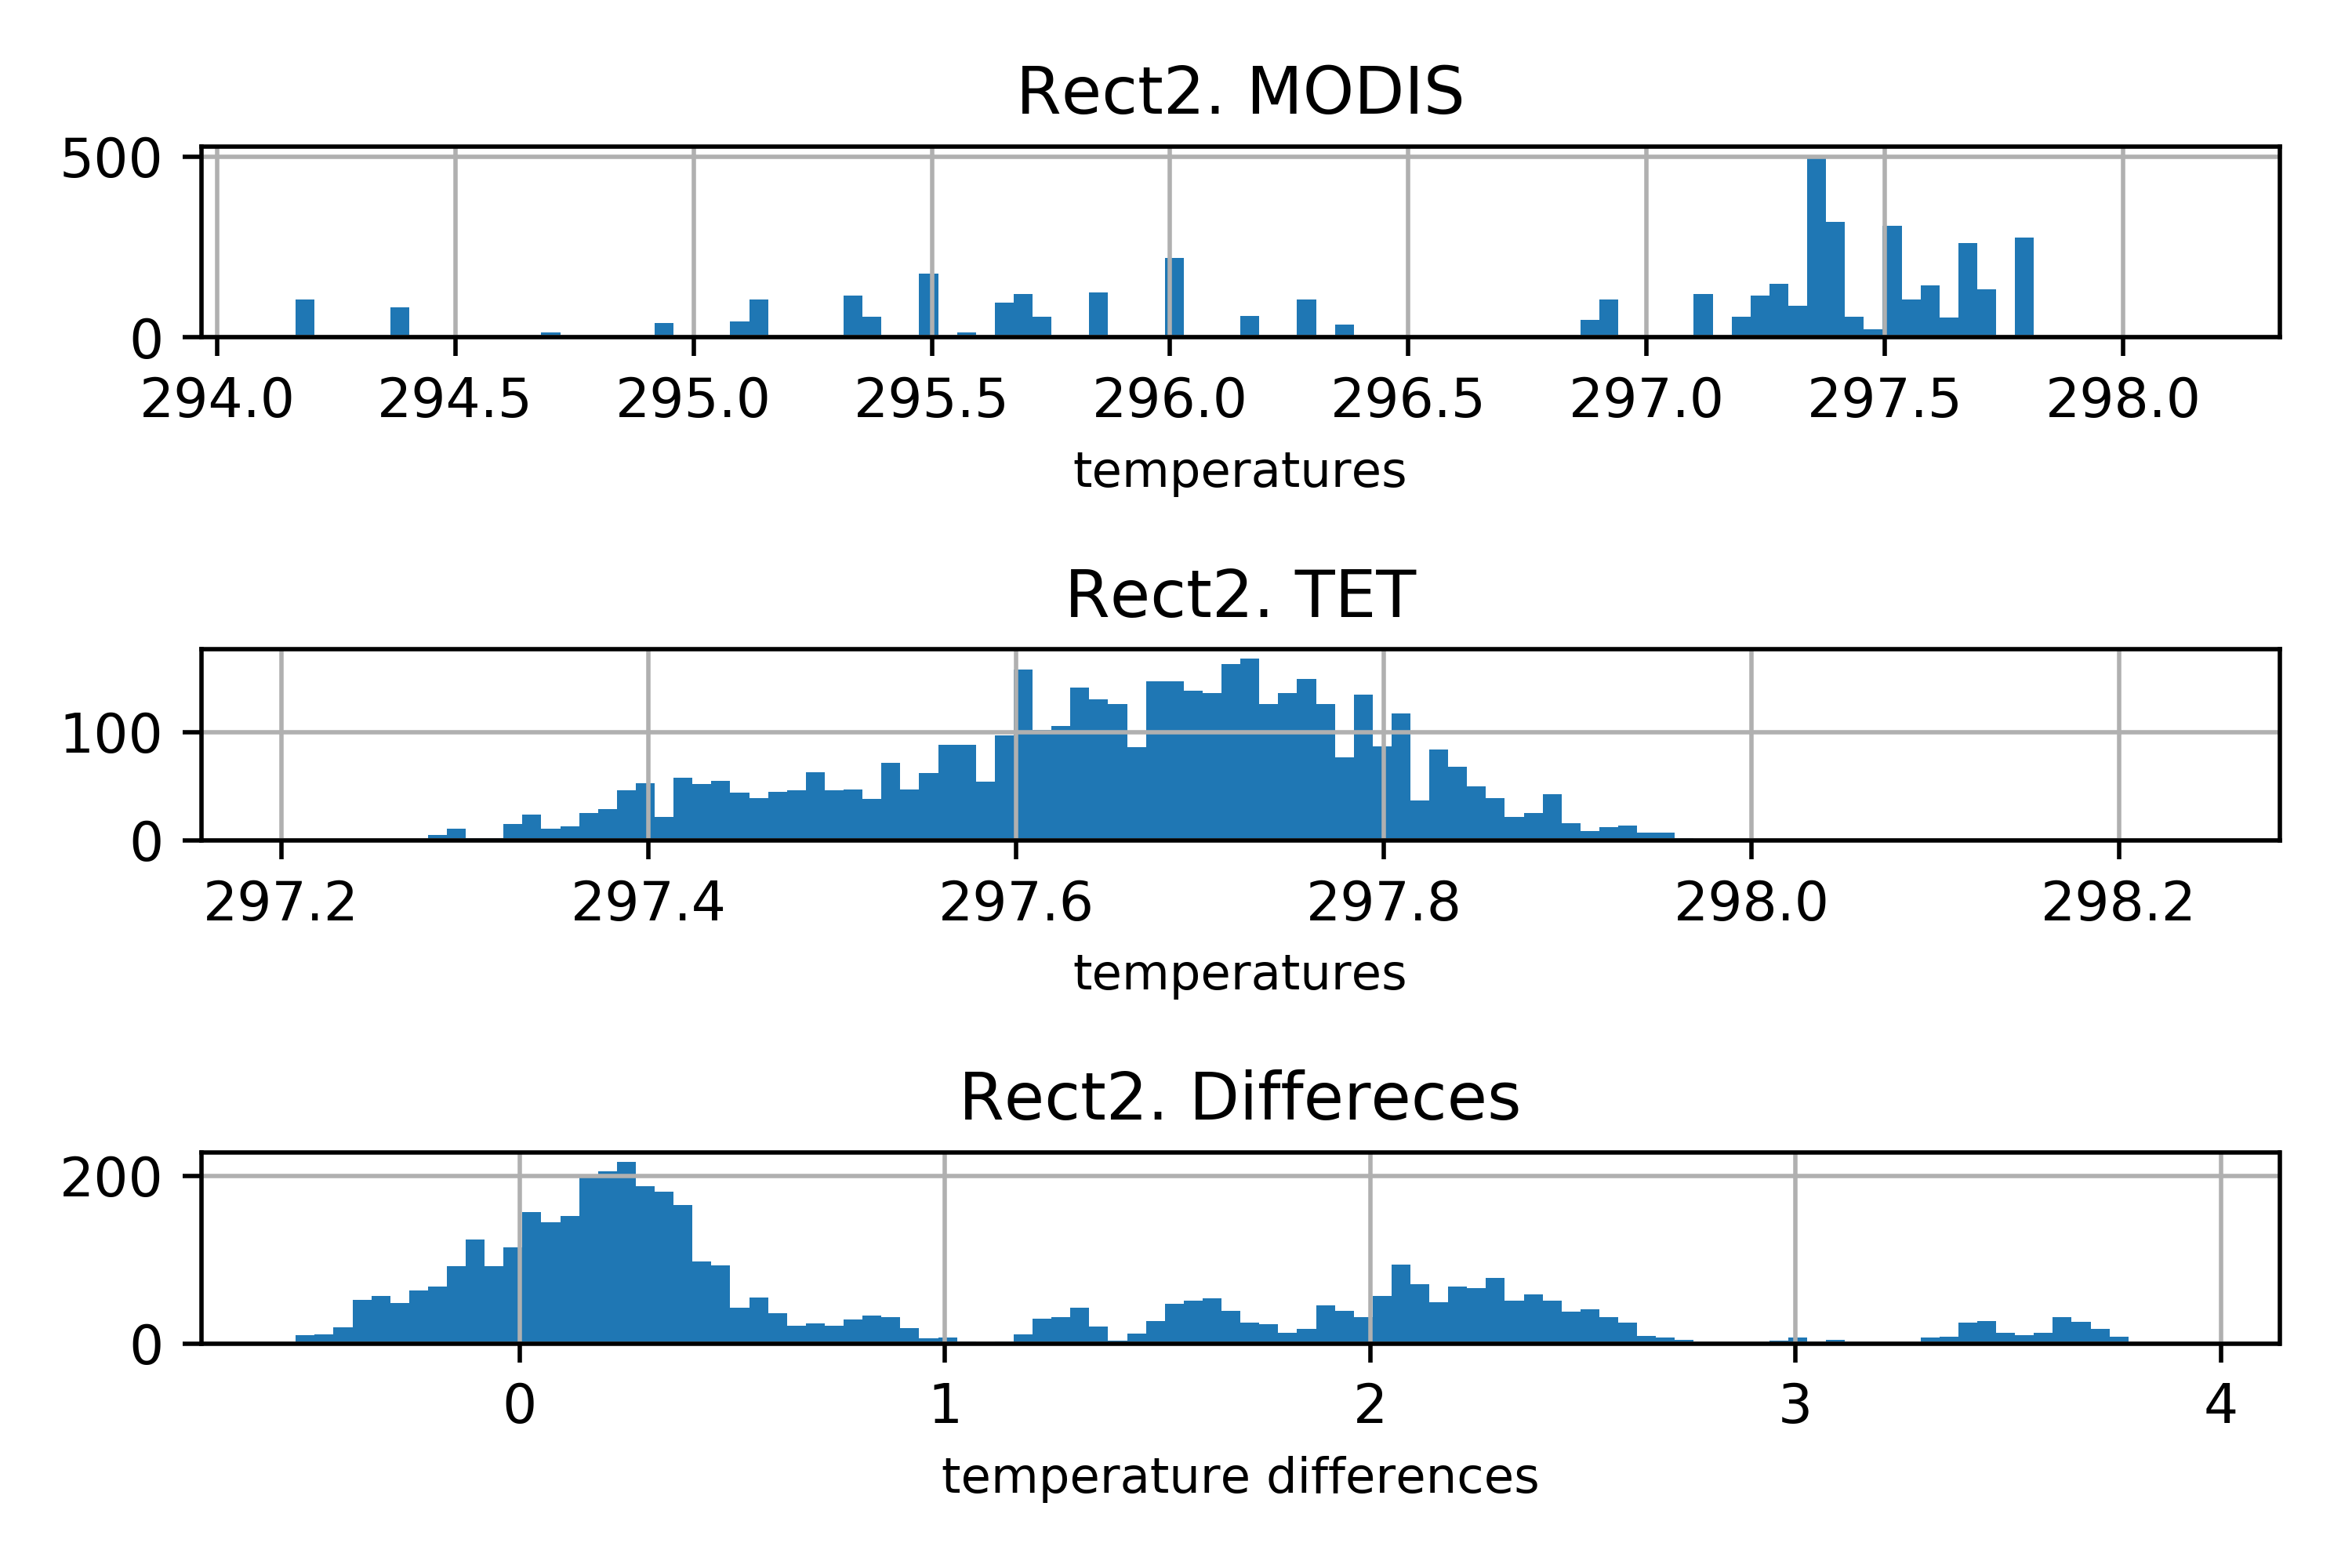
\includegraphics[width = 0.48\linewidth]{rect2_sc110.png}}

\hspace{0.5in}

\subfigure[Sub-area 3 with cale factor 1.00]{
\label{fig:hist_rect3_1}
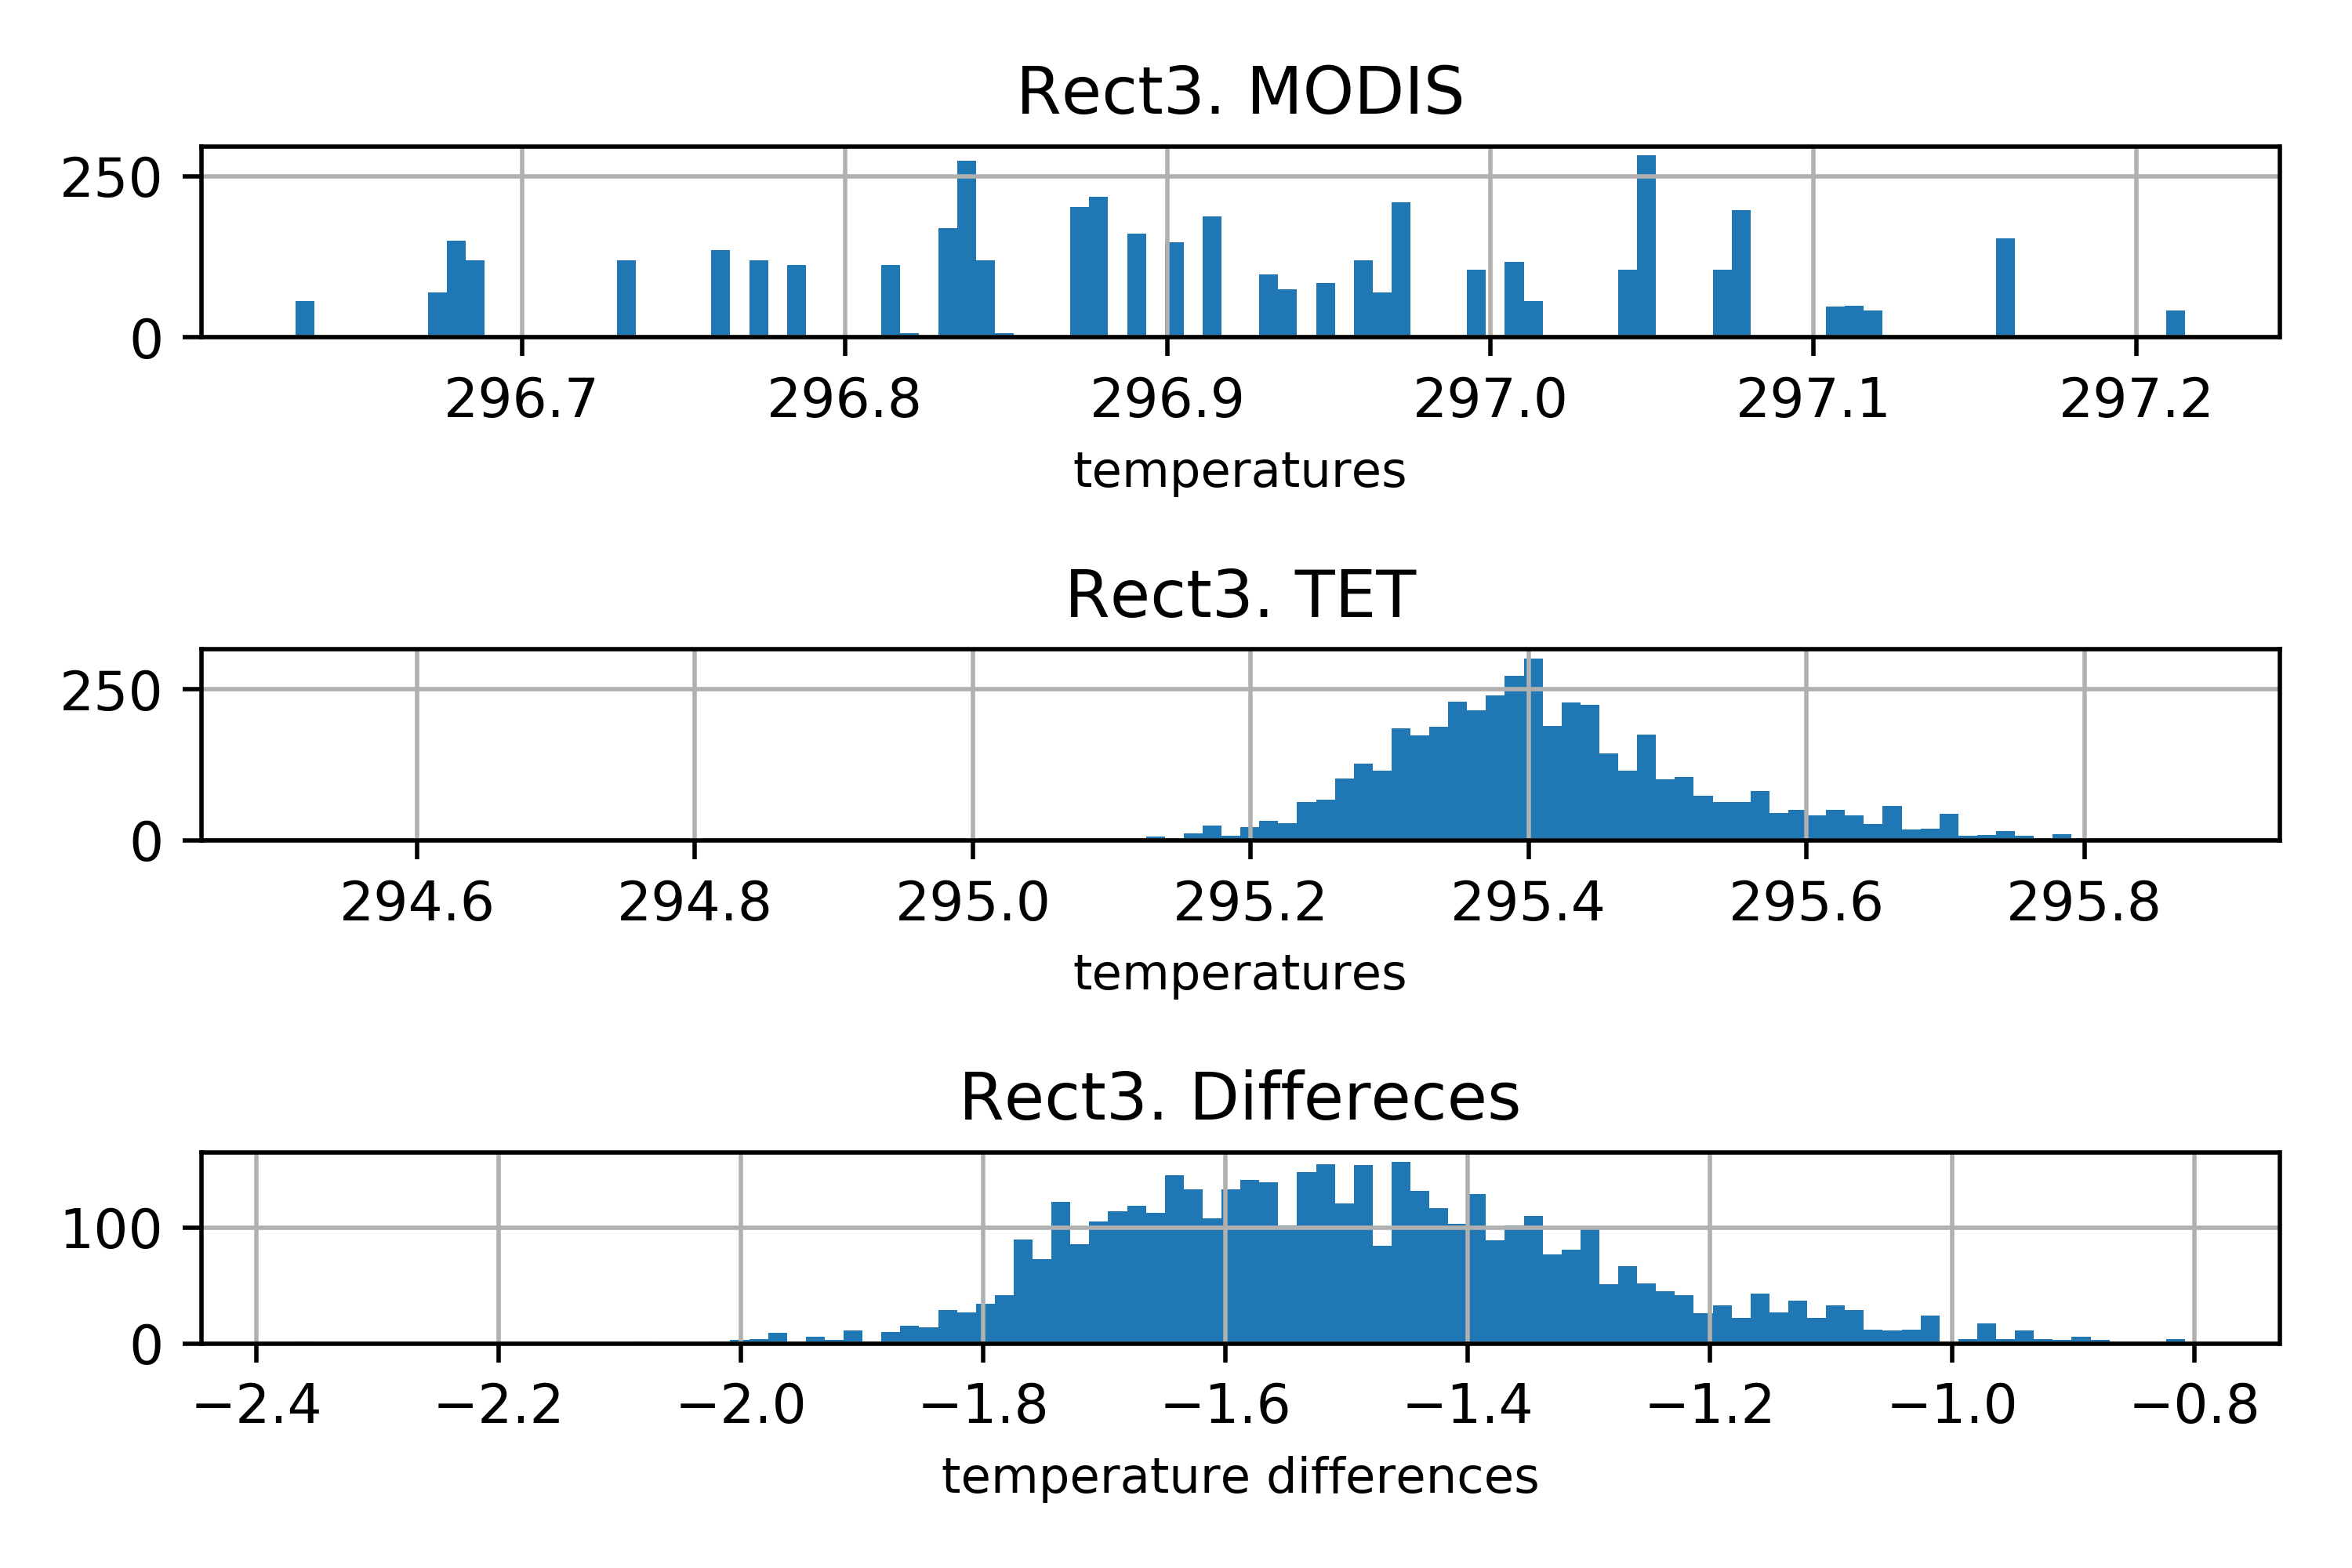
\includegraphics[width = 0.48\linewidth]{rect3_sc100.png}}
\vspace{0.1in}
\subfigure[Sub-area 3 with cale factor 1.10]{
\label{fig:hist_rect3_2}
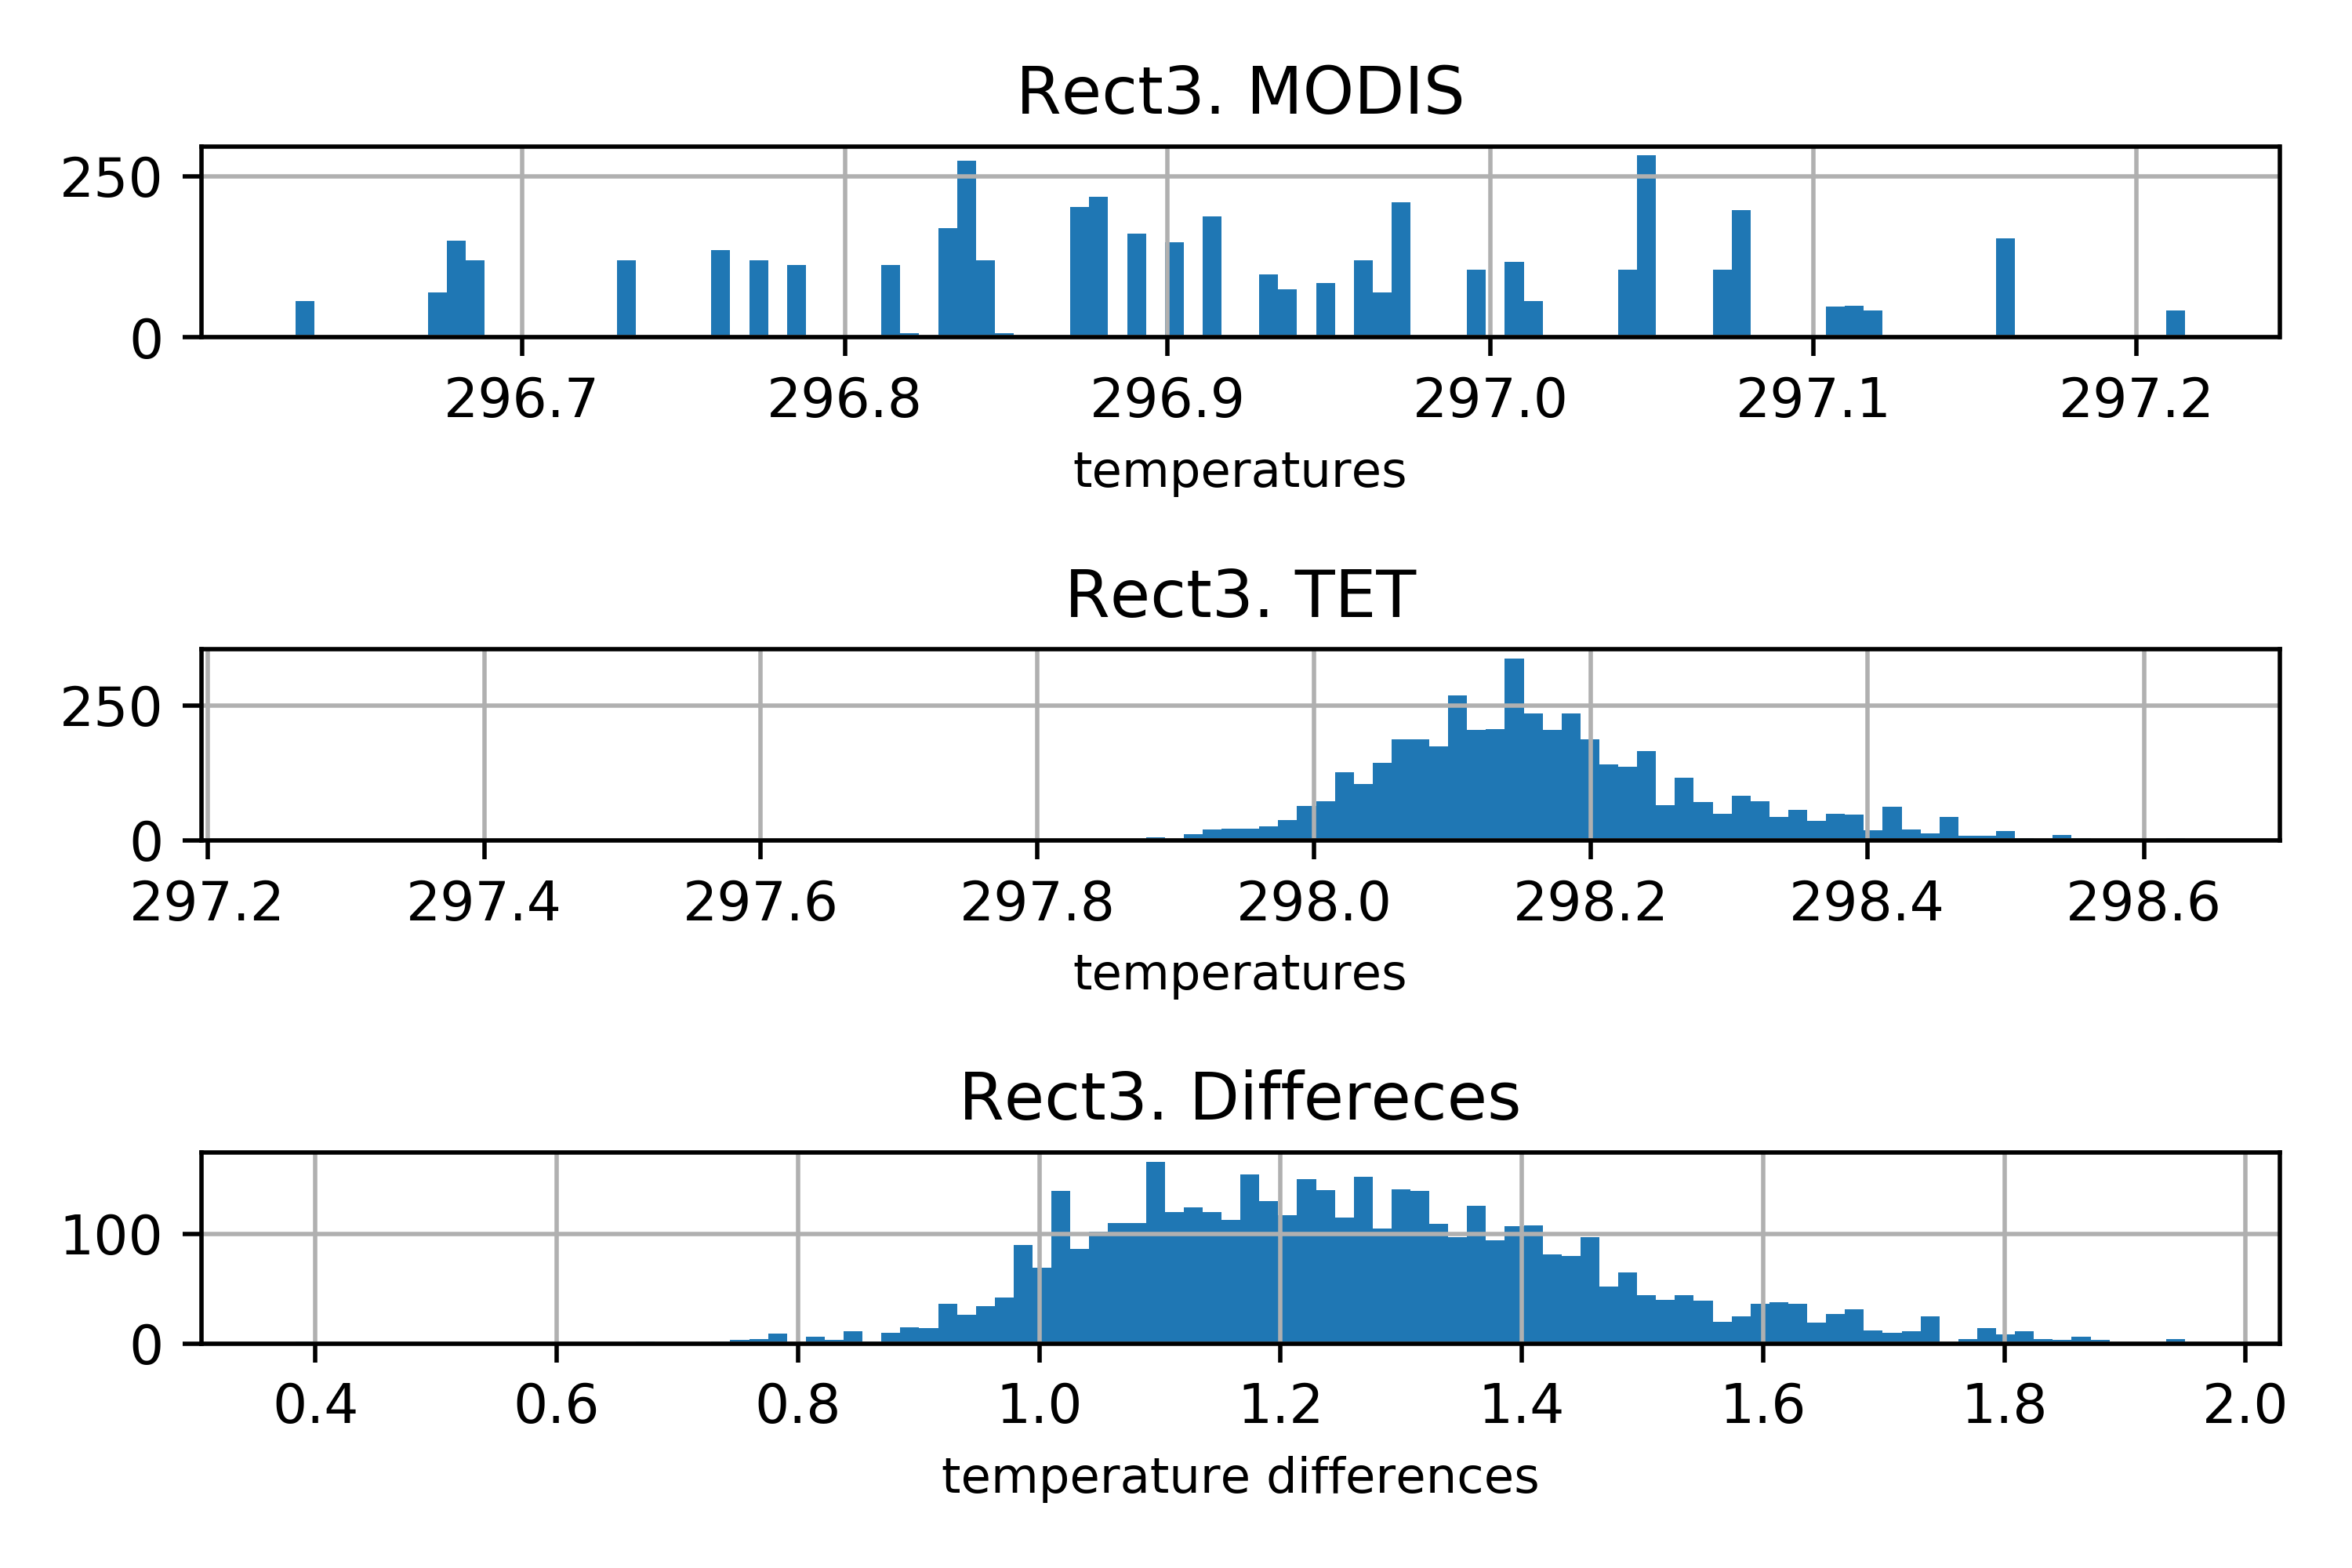
\includegraphics[width = 0.48\linewidth]{rect3_sc110.png}}

\hspace{0.5in}

\subfigure[Sub-area 4 with cale factor 1.00]{
\label{fig:hist_rect4_1}
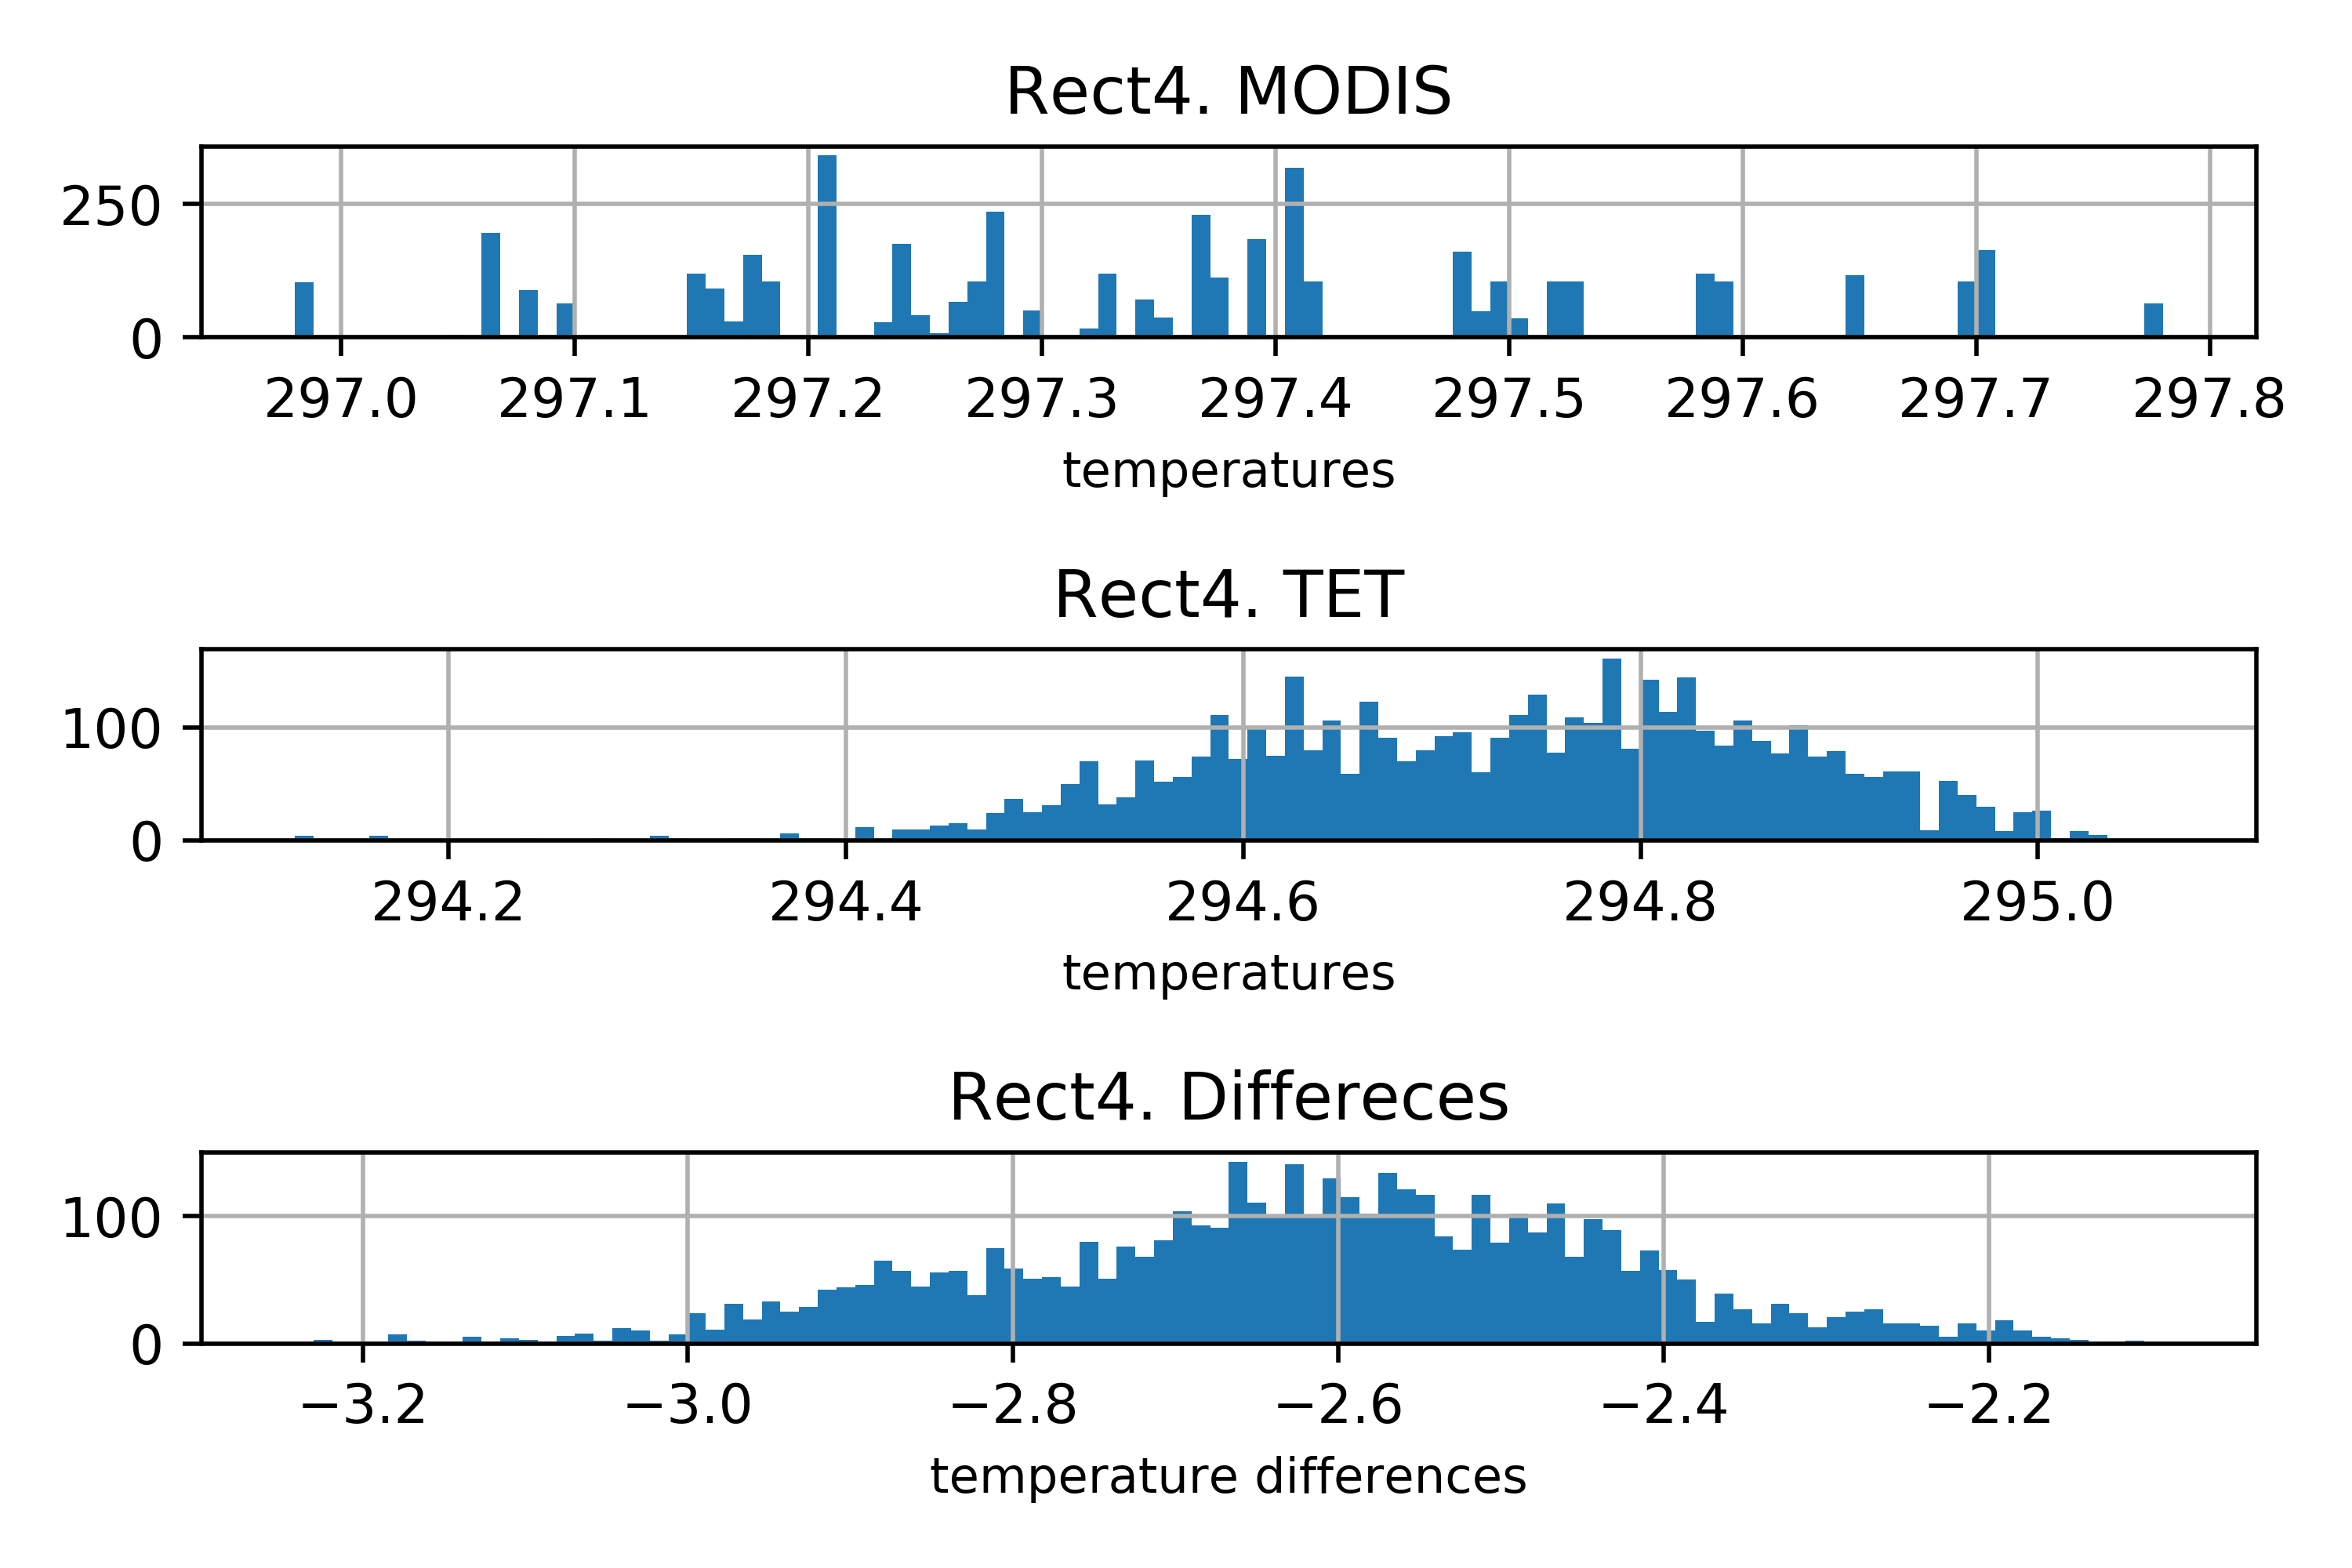
\includegraphics[width = 0.48\linewidth]{rect4_sc100.png}}
\vspace{0.1in}
\subfigure[Sub-area 4 with cale factor 1.10]{
\label{fig:hist_rect4_2}
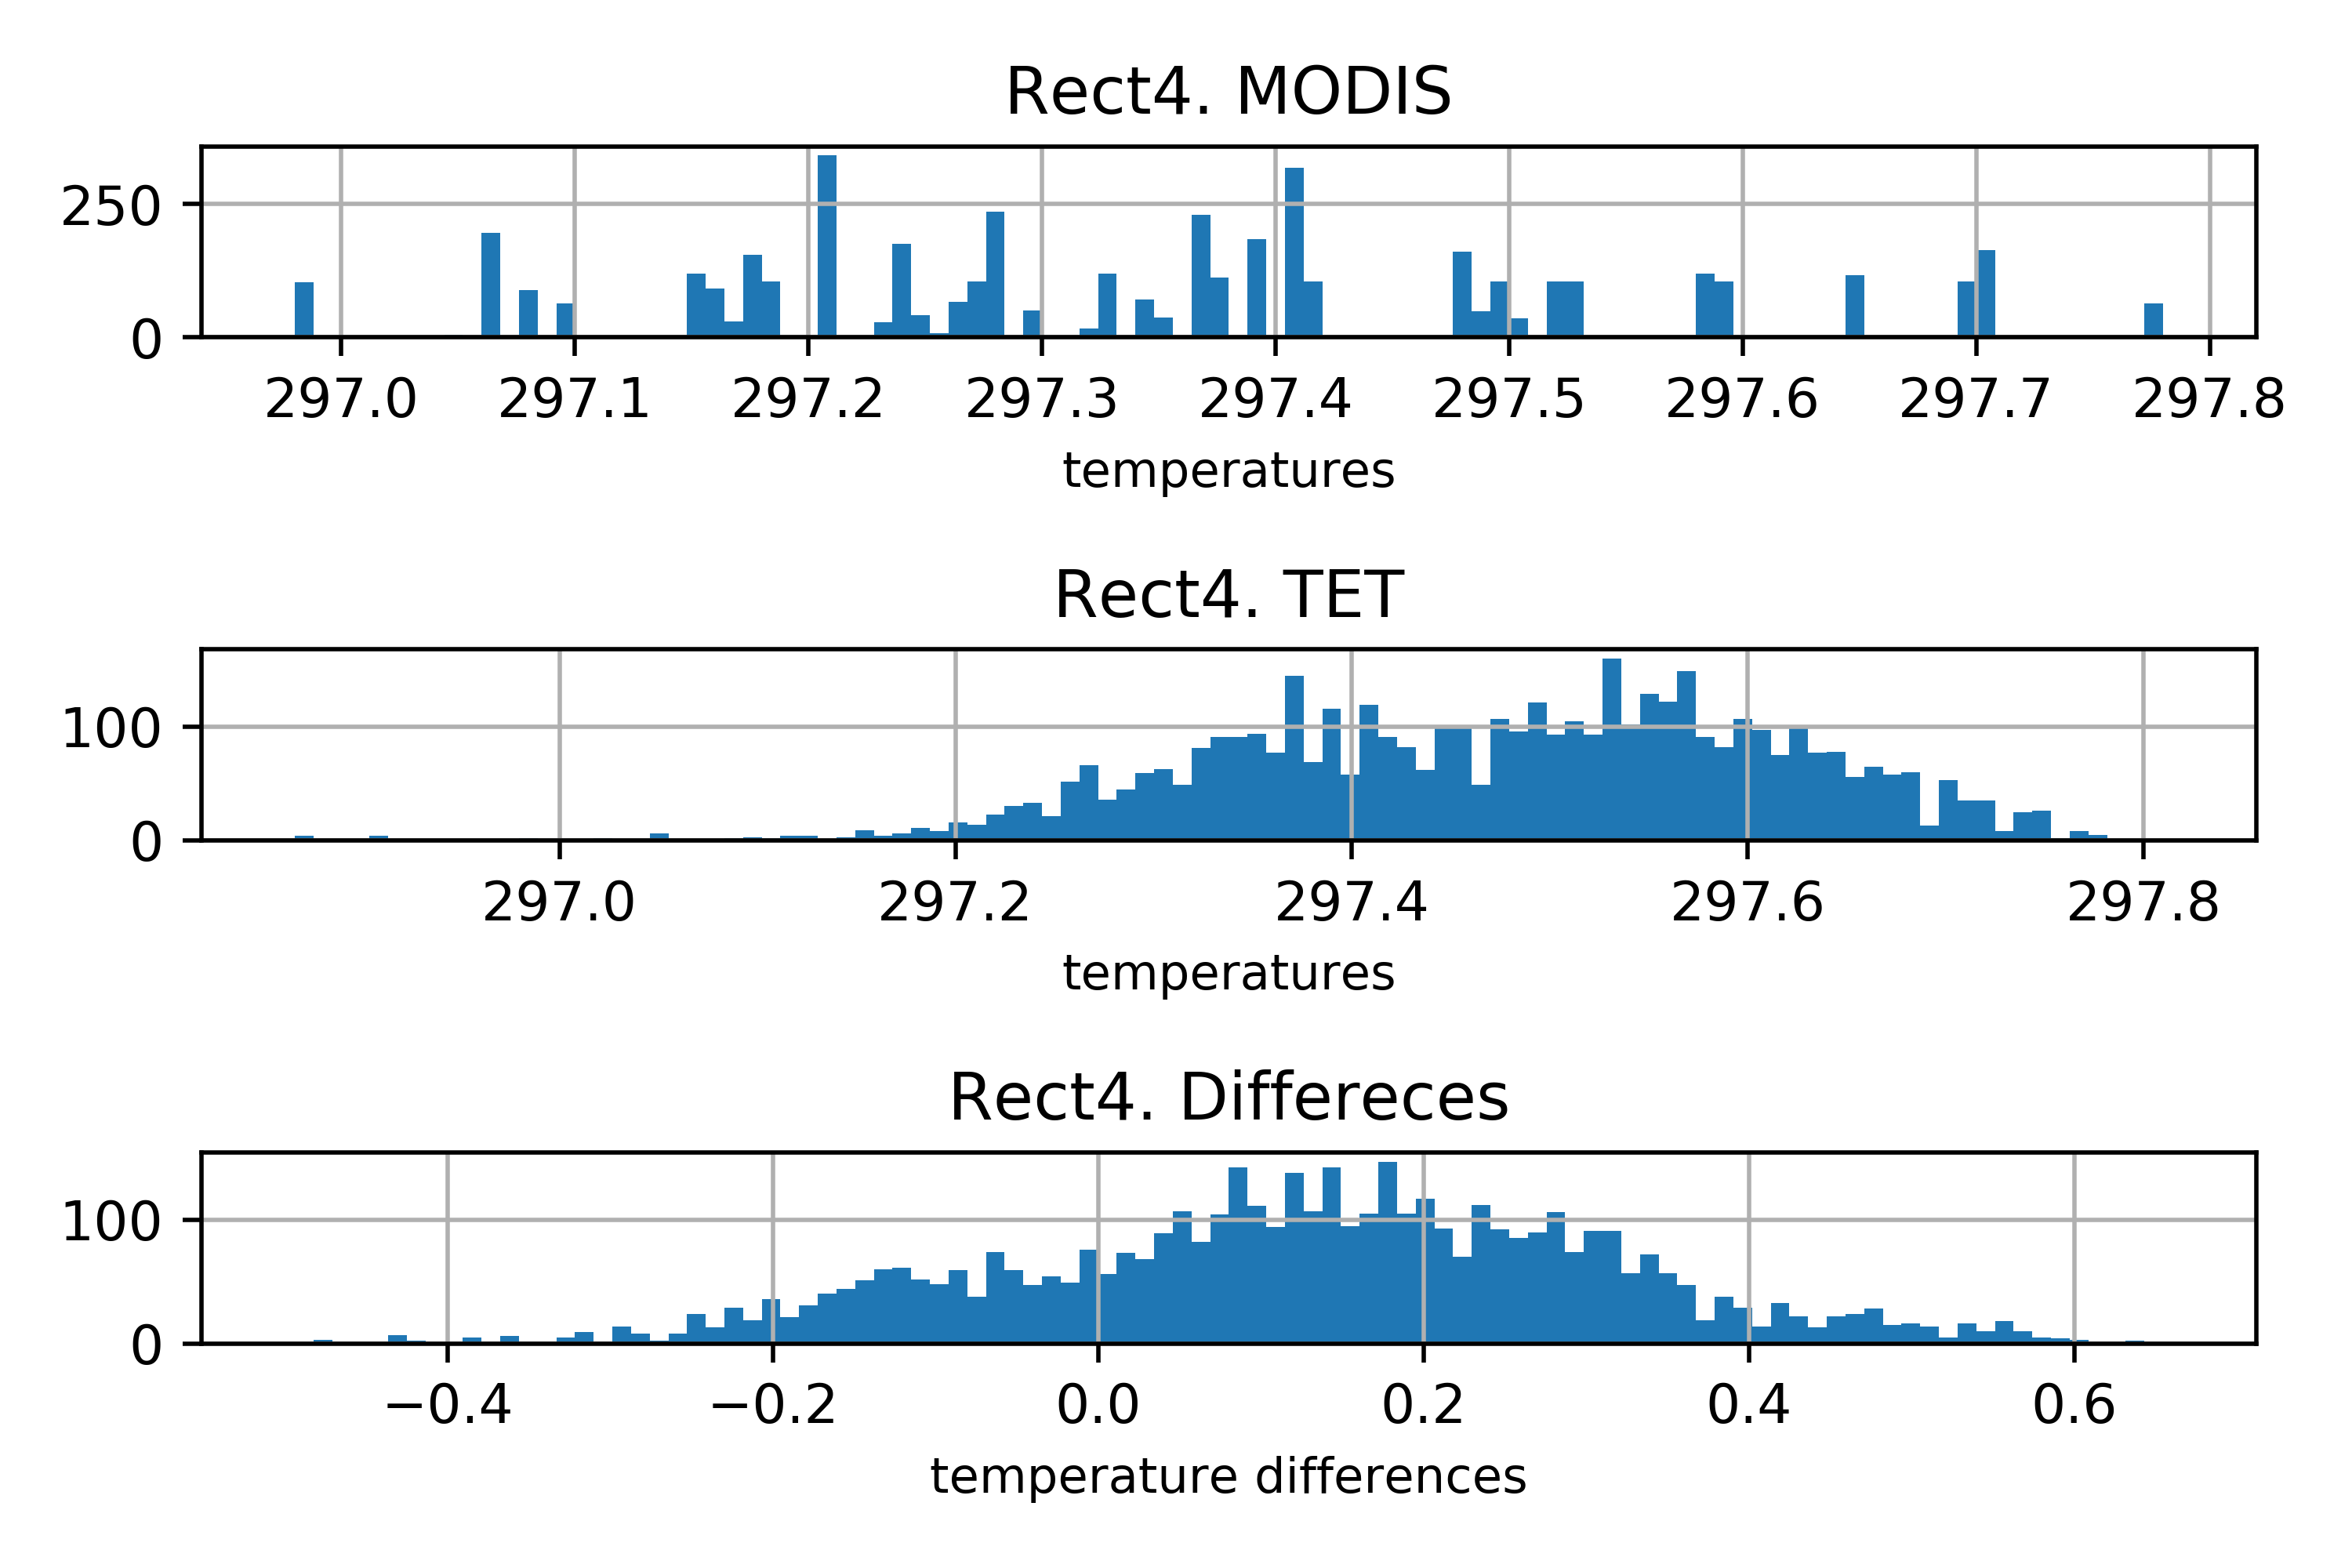
\includegraphics[width = 0.48\linewidth]{rect4_sc110.png}}

\caption{Histograms of MODIS SST, TET-1 MIR band imagry and their differences with different scale factor}
\label{fig:hist_rect_all}
\end{figure}

\noindent In Figure \ref{fig:hist_rect_all}, it is clear that the histograms of the same sub-area of MODIS SST are the same. For the TET-1 MIR band temperature maps with differnet scale factors, the shapes of the histograms of the same sub-area, which are the second row of each sub-figures, are almost identical. But looking carefully we will notice that for the histograms of TET-1 MIR band temperature map with different scale factors, the x-axes are shifted to the left, which means the pixel values of all pixels inside one sub-area are increased with a certain value. The same for the temperature differences between MODIS SST and the TET-1 MIR band temperature map. To make it more clear, two sub-areas are selected and their histograms with all the five scale factors are shown in Figure \ref{fig:rect1_sc_all} and Figure \ref{fig:rect4_sc_all}.\\

\begin{figure}[!htbp]
\centering
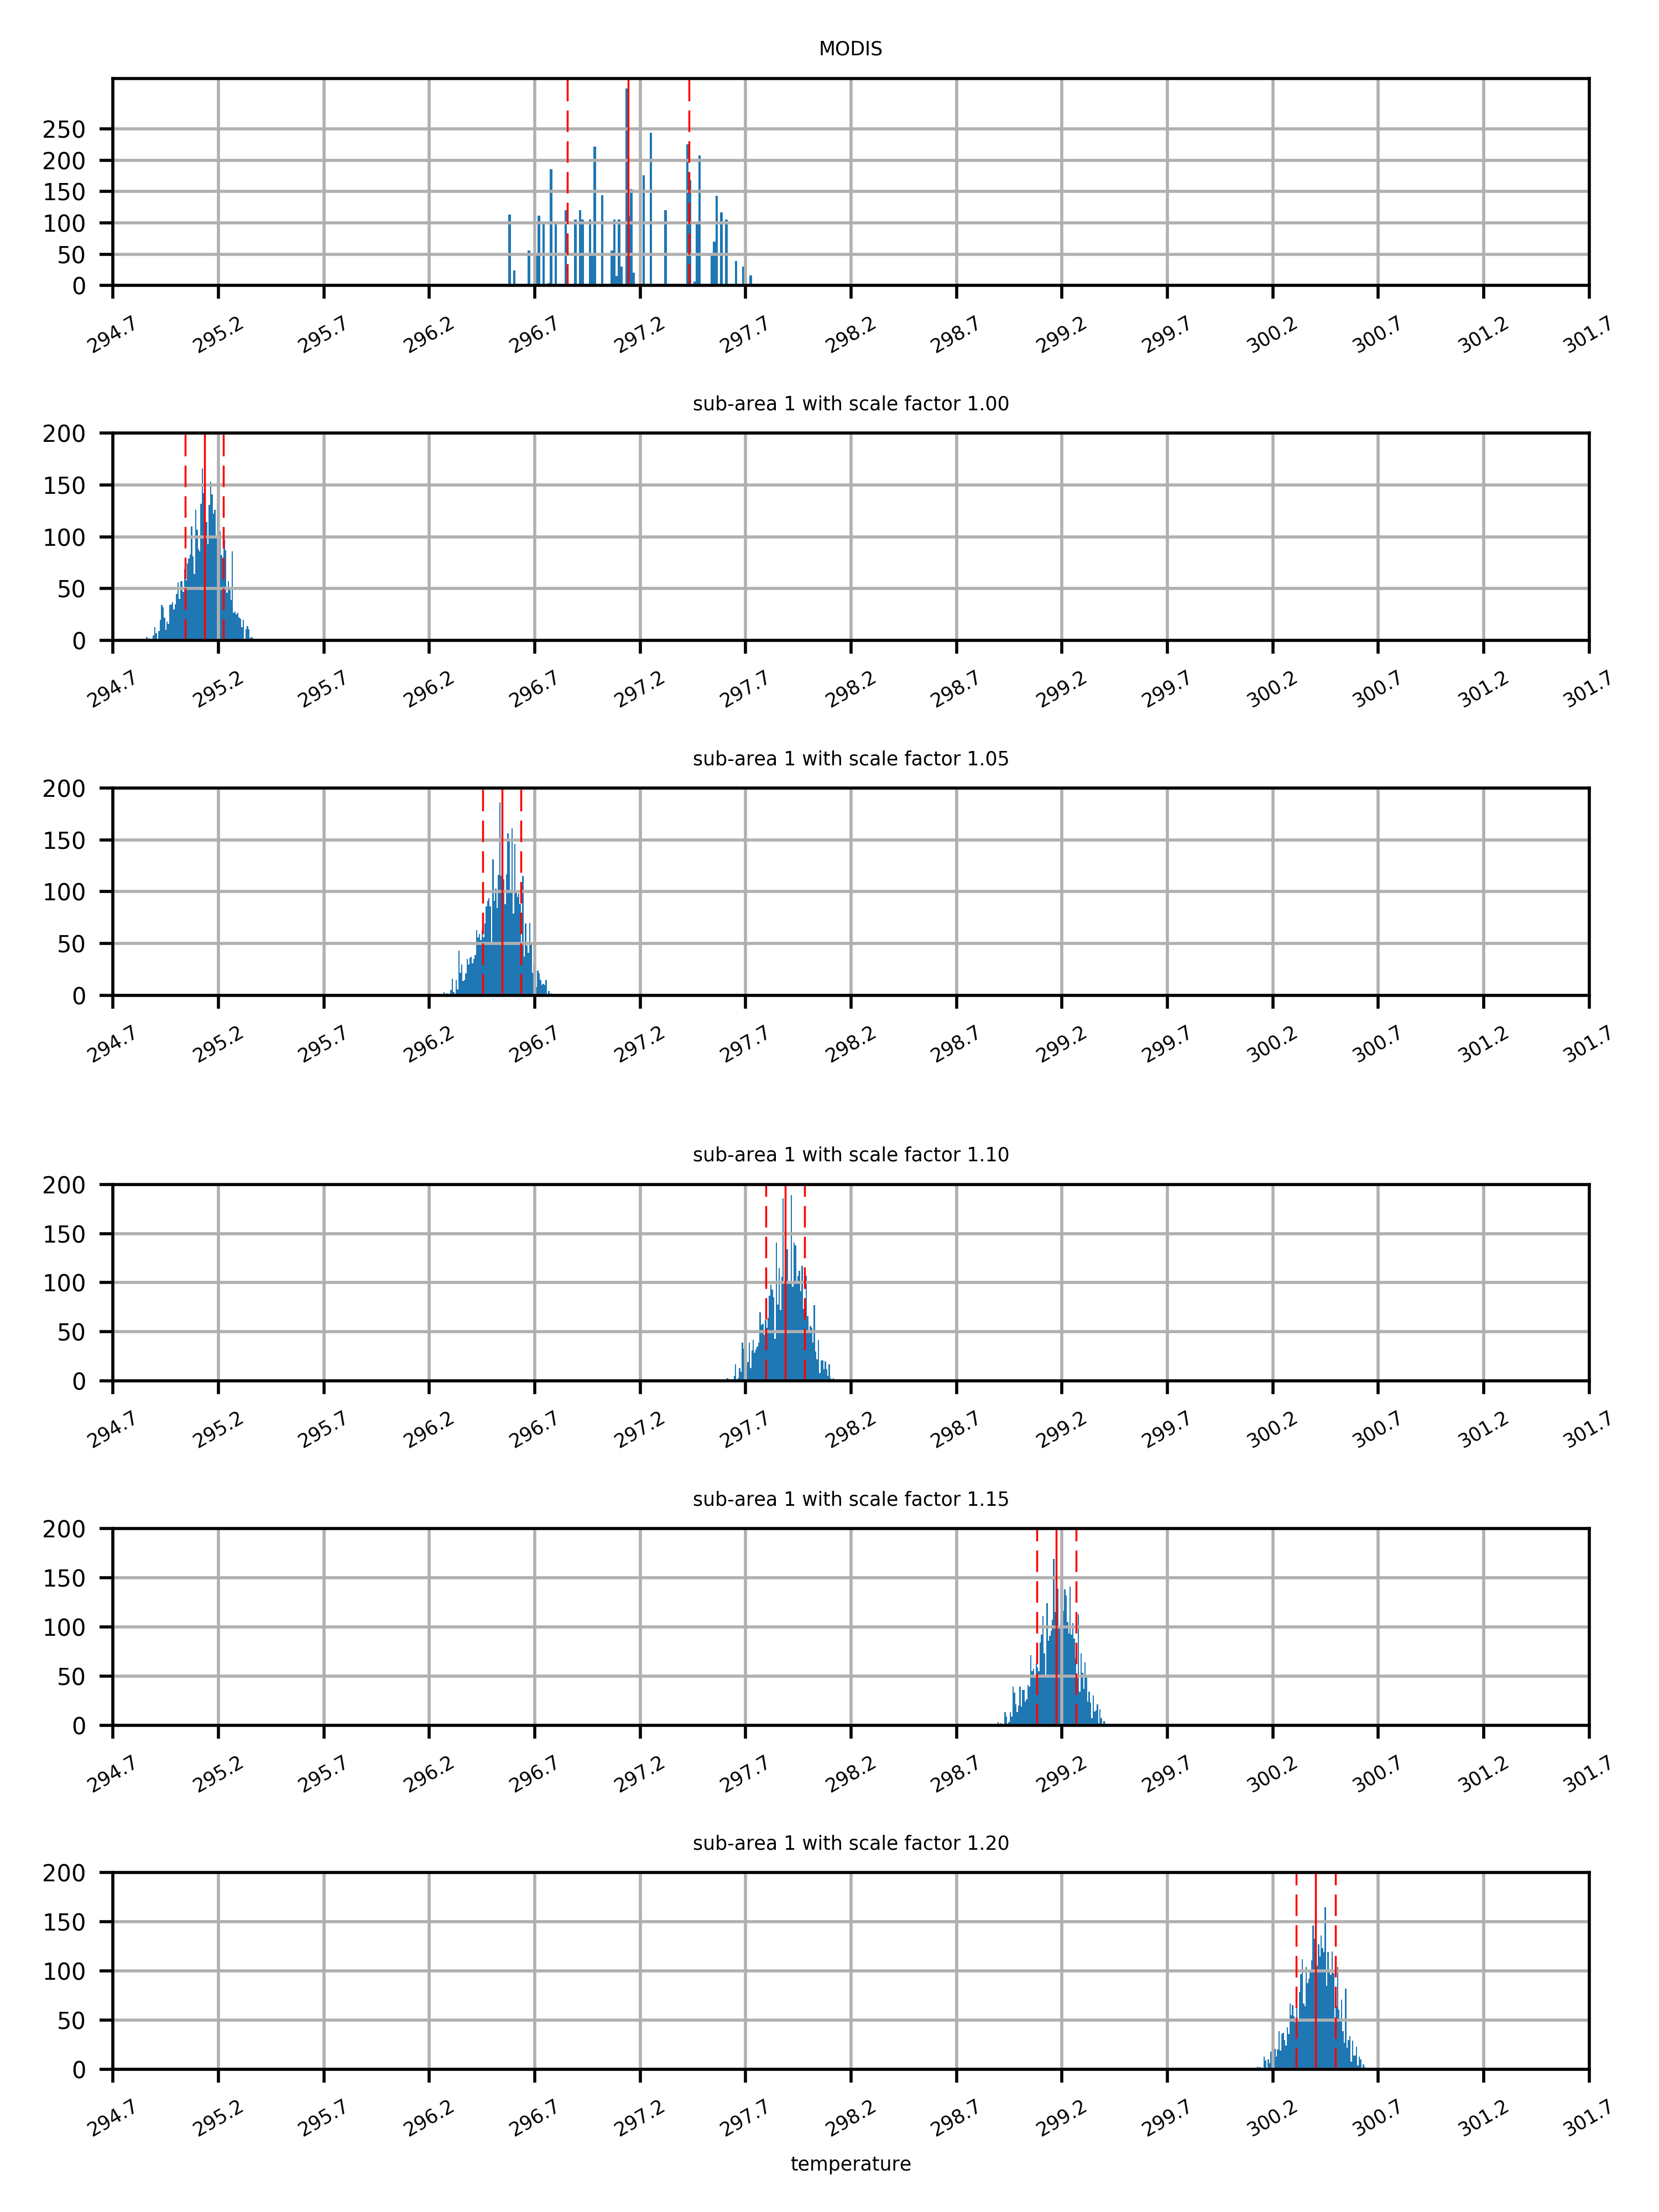
\includegraphics[width = 1.0\textwidth]{rect1_sc_all.png}
\caption{Histograms of MODIS SST and TET-1 MIR band imageries with all the five scale factors in sub-area 1. The red solid line in each histogram denotes the mean value and the red dashed line the standard deviation.}
\label{fig:rect1_sc_all}
\end{figure}

\begin{figure}[!htbp]
\centering
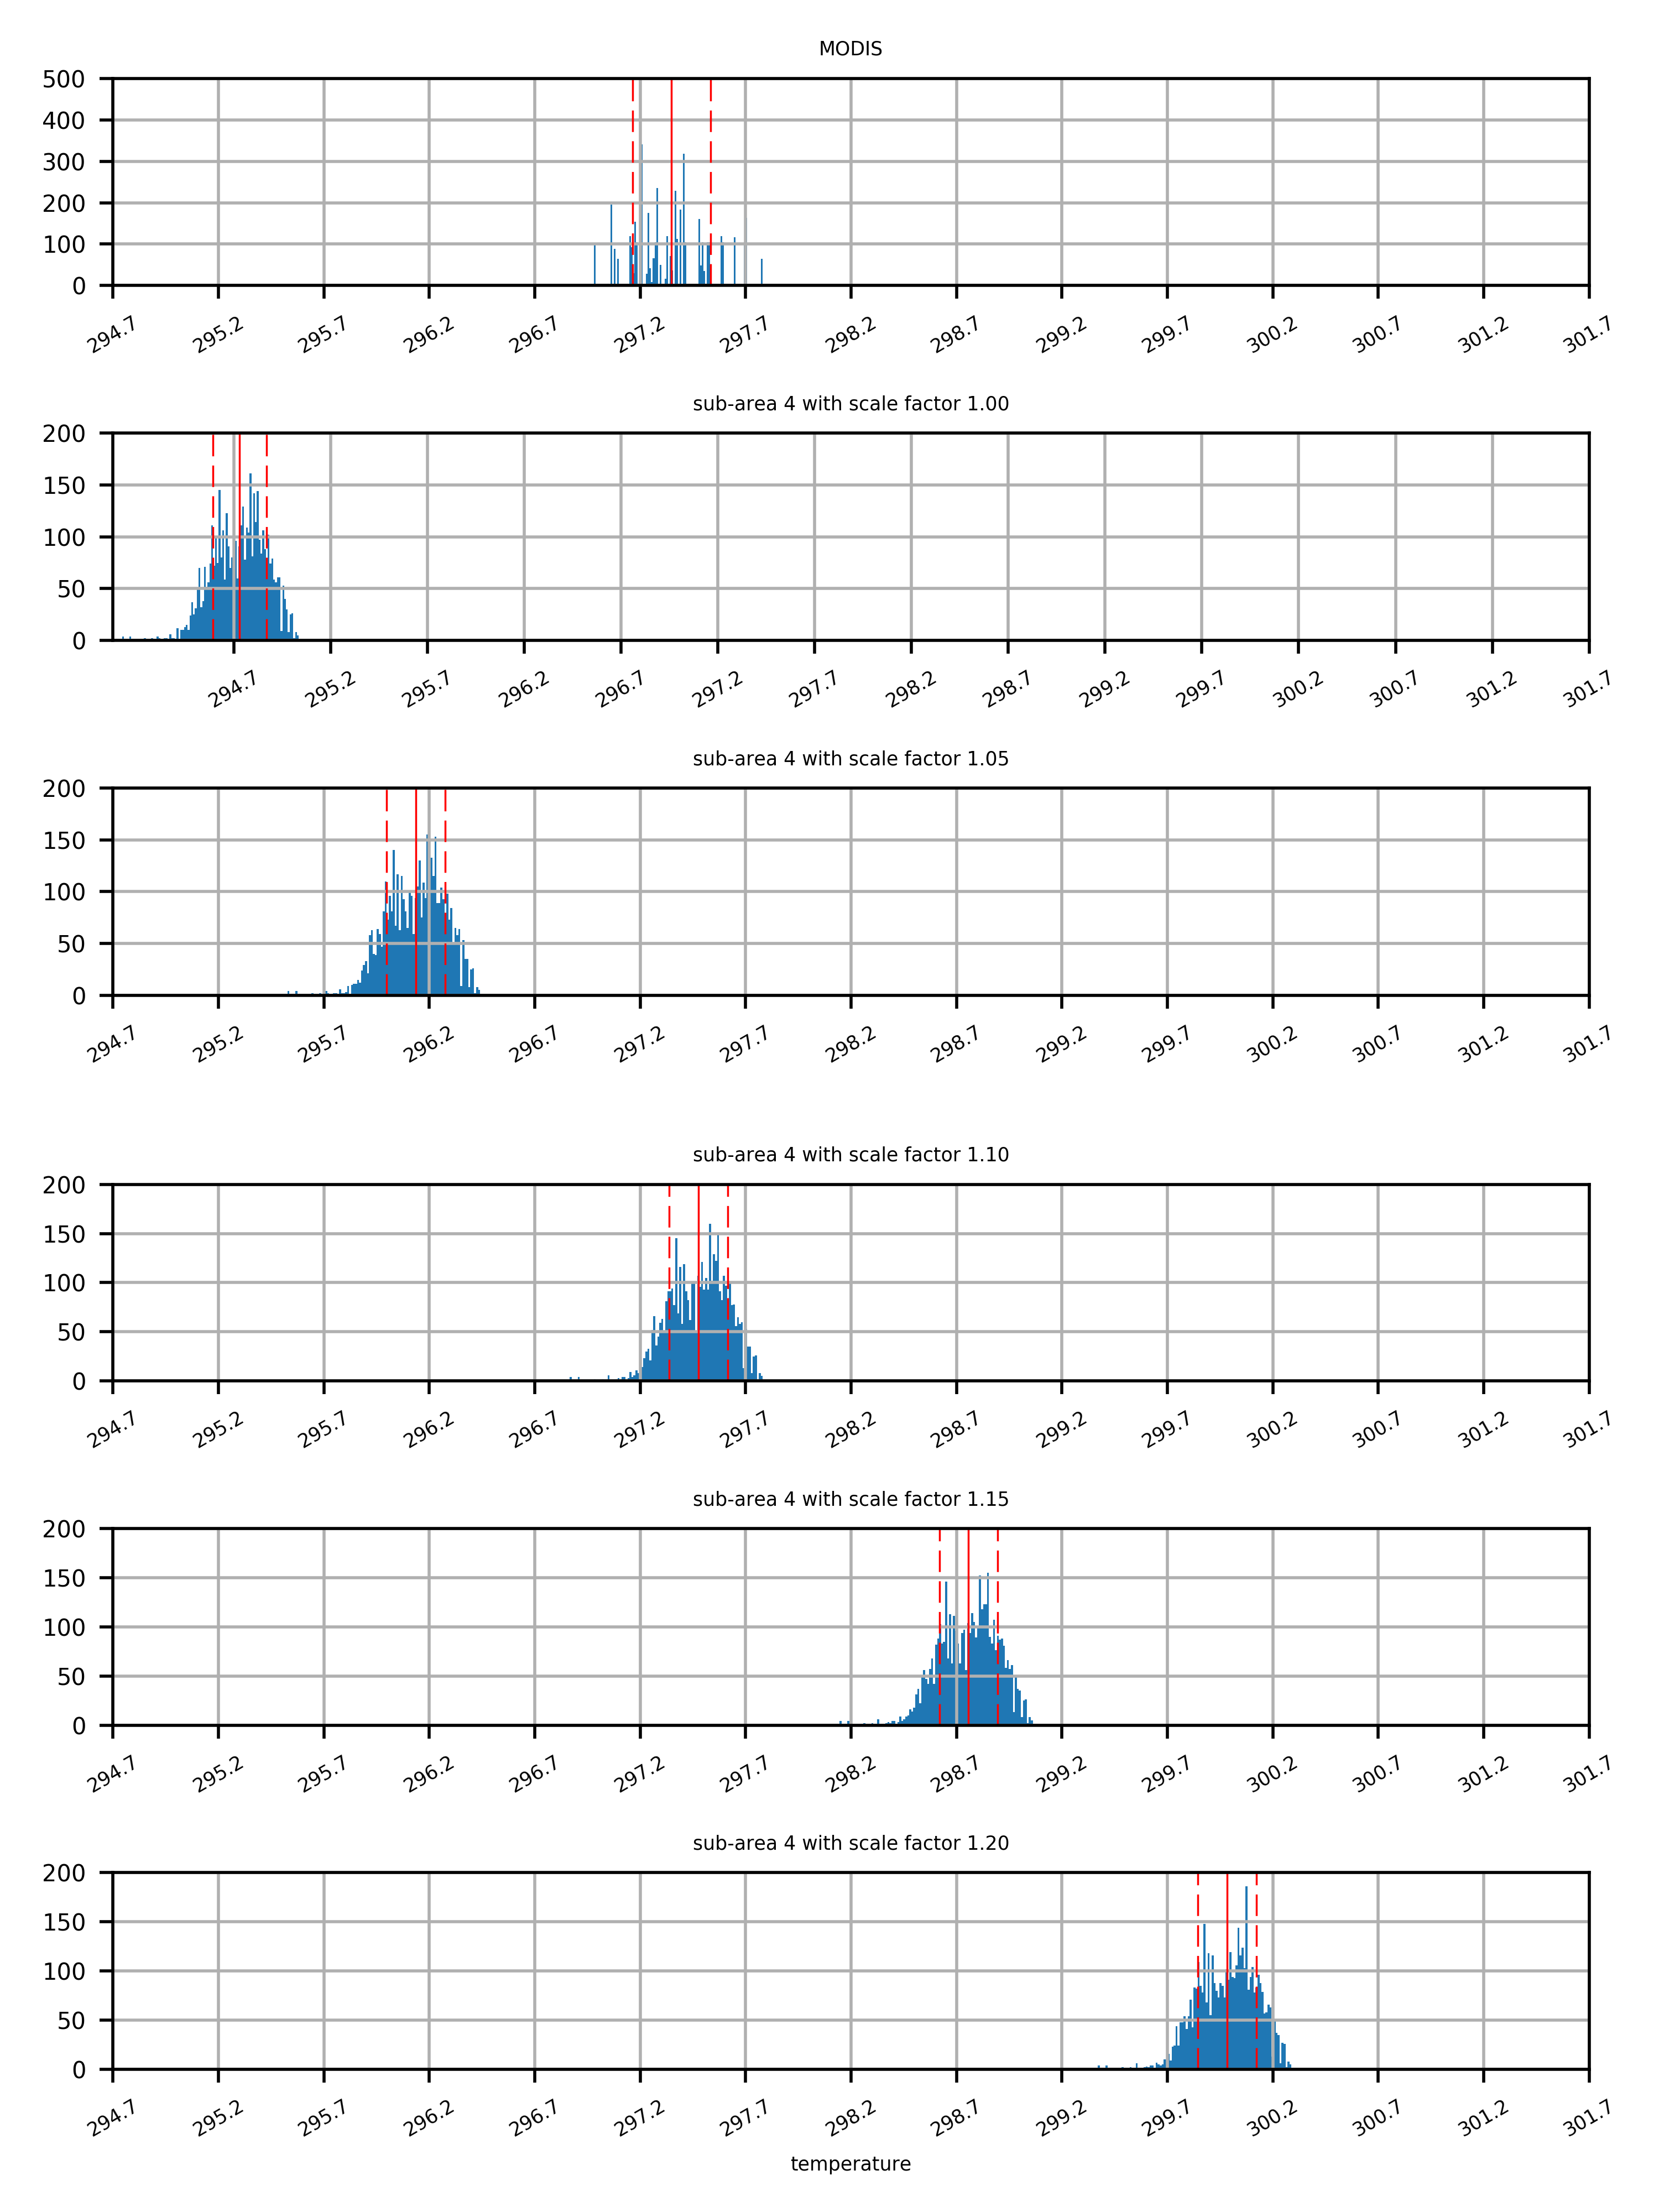
\includegraphics[width = 1.0\textwidth]{rect4_sc_all.png}
\caption{Histograms of MODIS SST and TET-1 MIR band imageries with all the five scale factors in sub-area 4. The red solid line in each histogram denotes the mean value and the red dashed line the standard deviation.}
\label{fig:rect4_sc_all}
\end{figure}

\noindent Figure \ref{fig:rect1_sc_all} and Figure \ref{fig:rect4_sc_all} obviously show that with the increment the scale factor, the histograms of the sub-areas will be shifted to the right while the shapes are almost unchanged. The mean temperature of each histogram acts as a linear function of scale factor while the standard deviations are very stable, which means the shapes of the histograms are keeping unchanged. Consequently, the mean temperature of all pixels within one sub-area can be used as representative for this sub-area and show how temperatures vary with the change of scale factor.\\

\noindent But we do not use only the mean temperature of one sub-area. As stated in Section 4.1.1, the mean temperature over all the sub-areas will be calculated to compare with the same value of MODIS SST. The histograms of pixels located inside all the sub-areas are given in Figure \ref{fig:hist_all_rect} and Figure \ref{fig:rect_all_sc_all}. For MODIS SST, due to the reasons of upsampling, noisy and missing value etc, its histograms of the sub-areas are sparse and concentrate in fewer values. Its shape is a bit skewed left but its main part is symmetric. Furthermore, the main part of the histogram of all sub-areas of MODIS SST shares the similar shape with the histograms of all sub-areas of TET-1 MIR band surface temperature map. For TET-1 MIR band surface temperature map, the behavior of histograms of all sub-areas is the same as the histograms of individual sub-area as stated before. Hence it is reasonable and reliable to use the mean temperature over all the sub-areas in both MODIS SST and TET-1 surface temperature product to do the comparison instead of using the histogram all the time.\\

\begin{figure}[!htbp]
\centering
\subfigure[Scale factor 1.00]{
\label{fig:hist_rect_all_1}
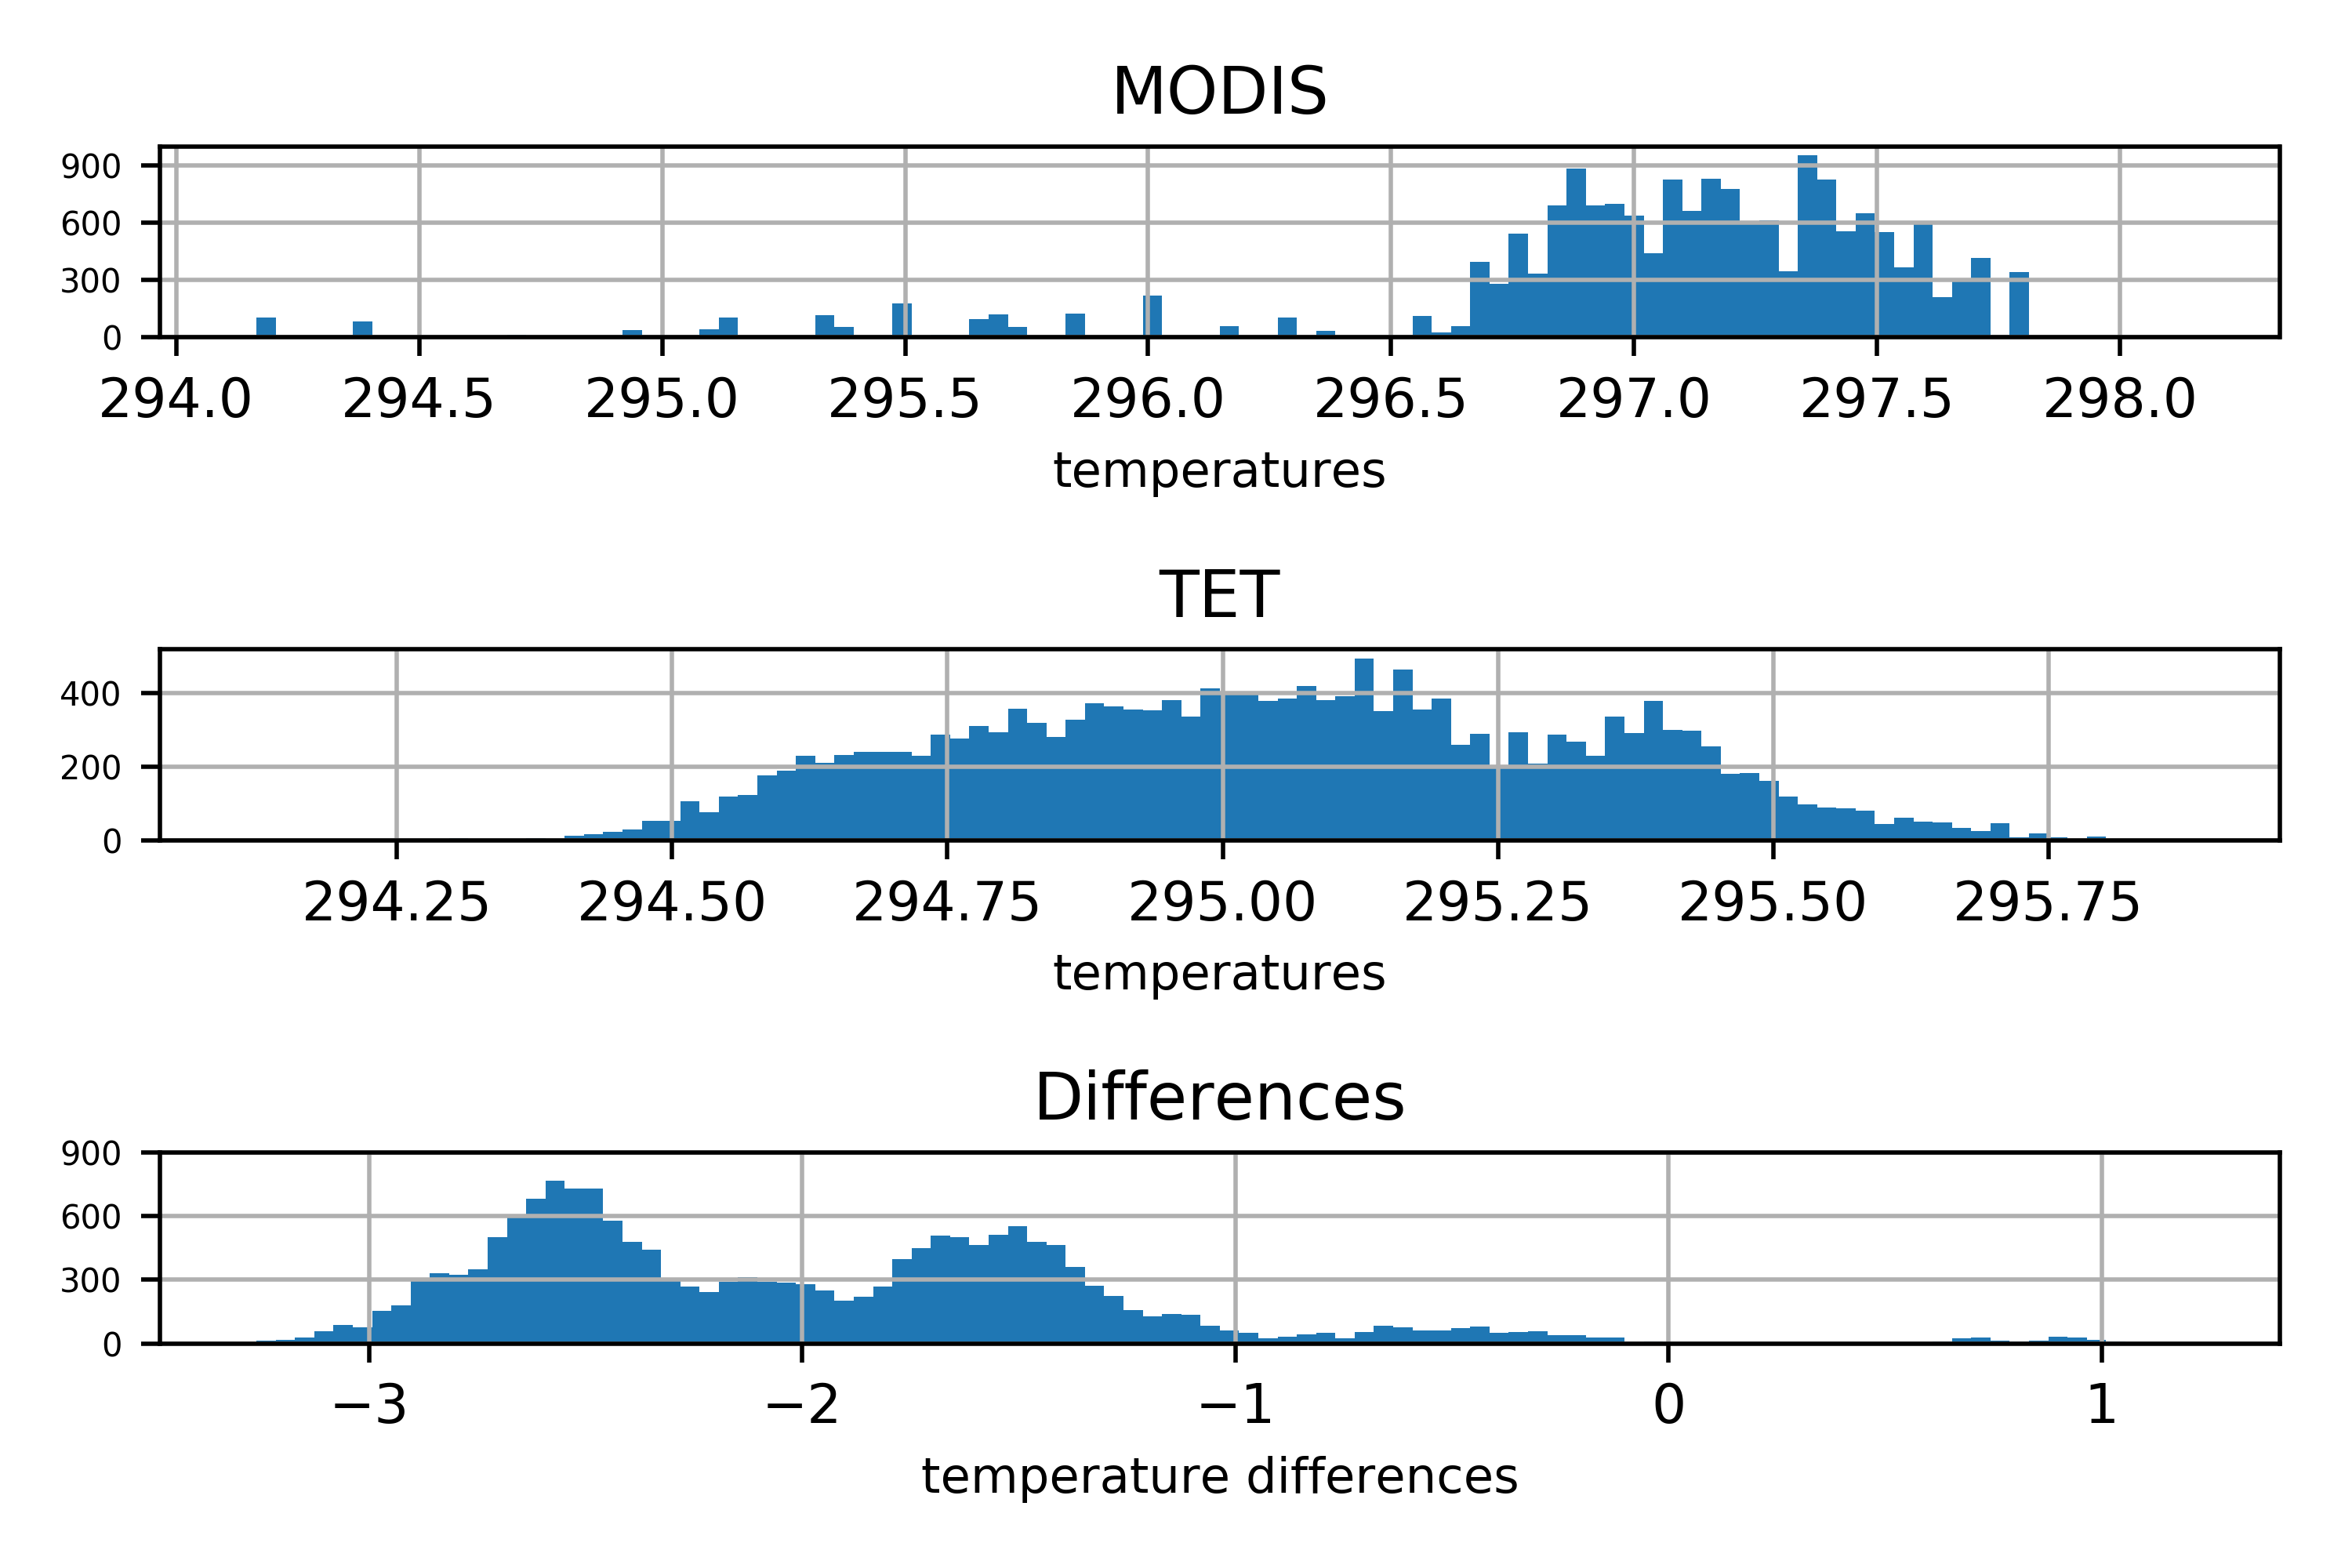
\includegraphics[width = 0.48\linewidth]{rect_all_sc100.png}}
\vspace{0.1in}
\subfigure[Scale factor 1.10]{
\label{fig:hist_rect_all_2}
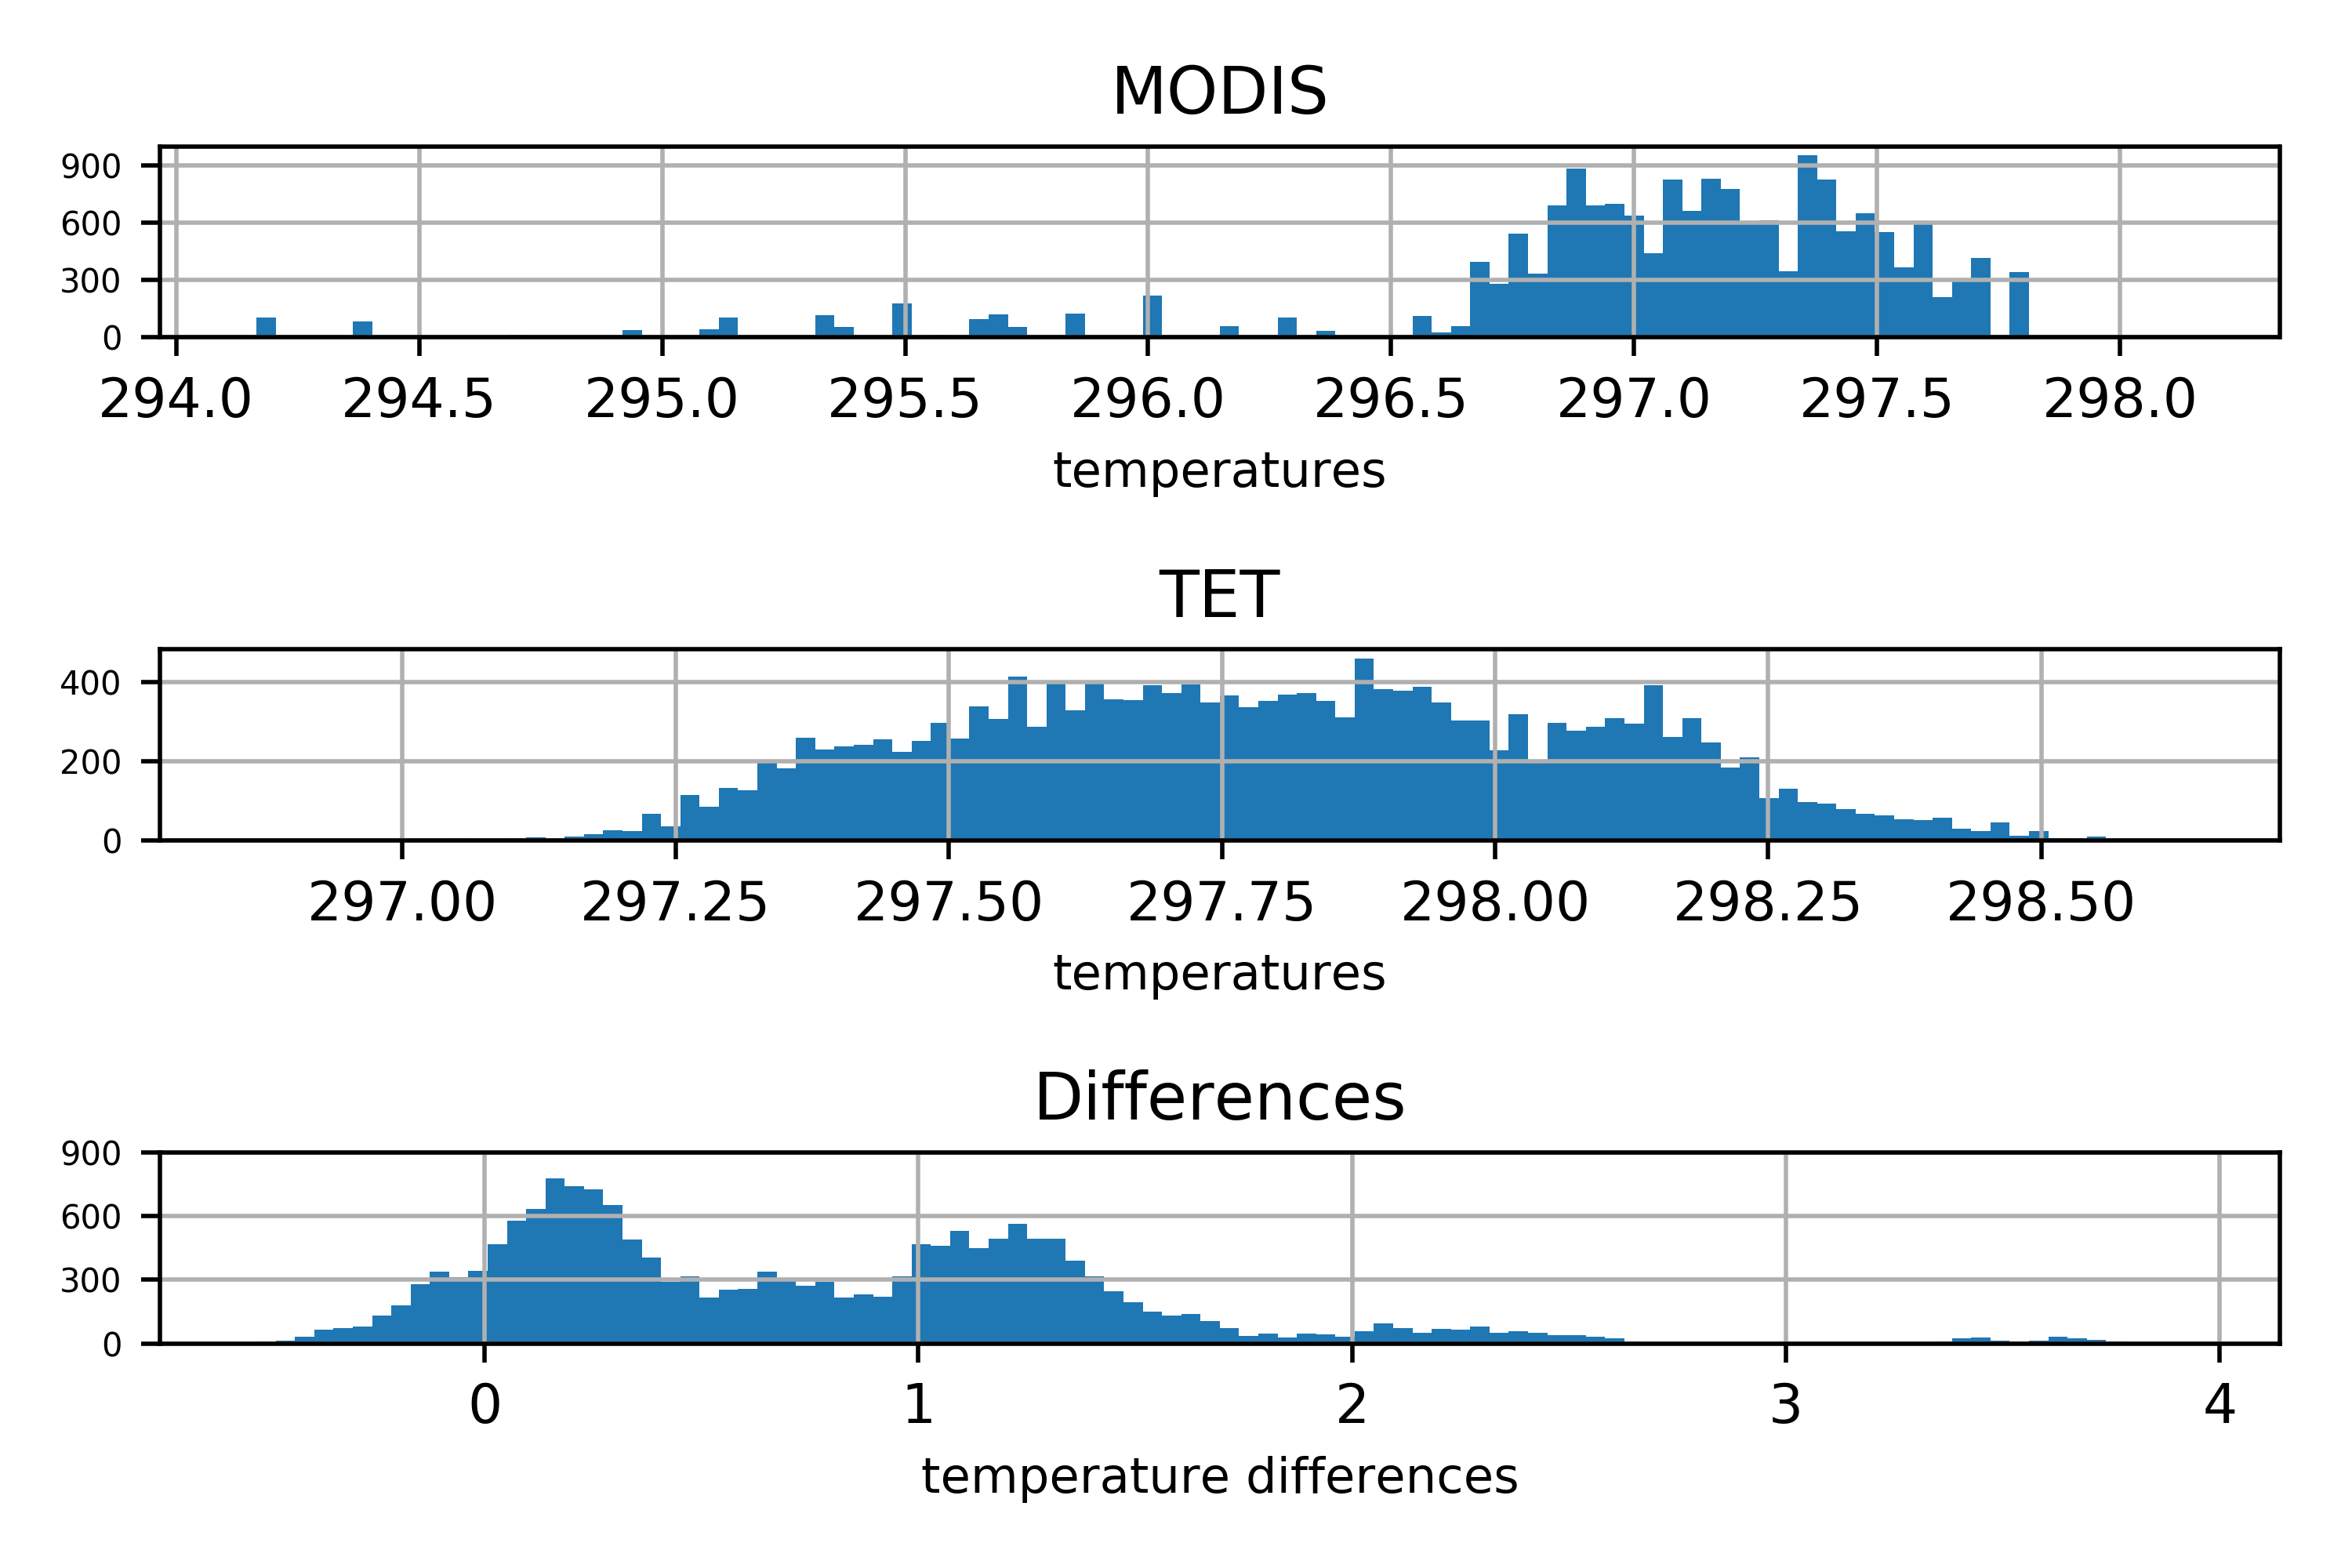
\includegraphics[width = 0.48\linewidth]{rect_all_sc110.png}}
\caption{Histograms of all sub-areas of MODIS SST, TET-1 MIR band imagry and their differences with different scale factor}
\label{fig:hist_all_rect}
\end{figure}

\begin{figure}[!htbp]
\centering
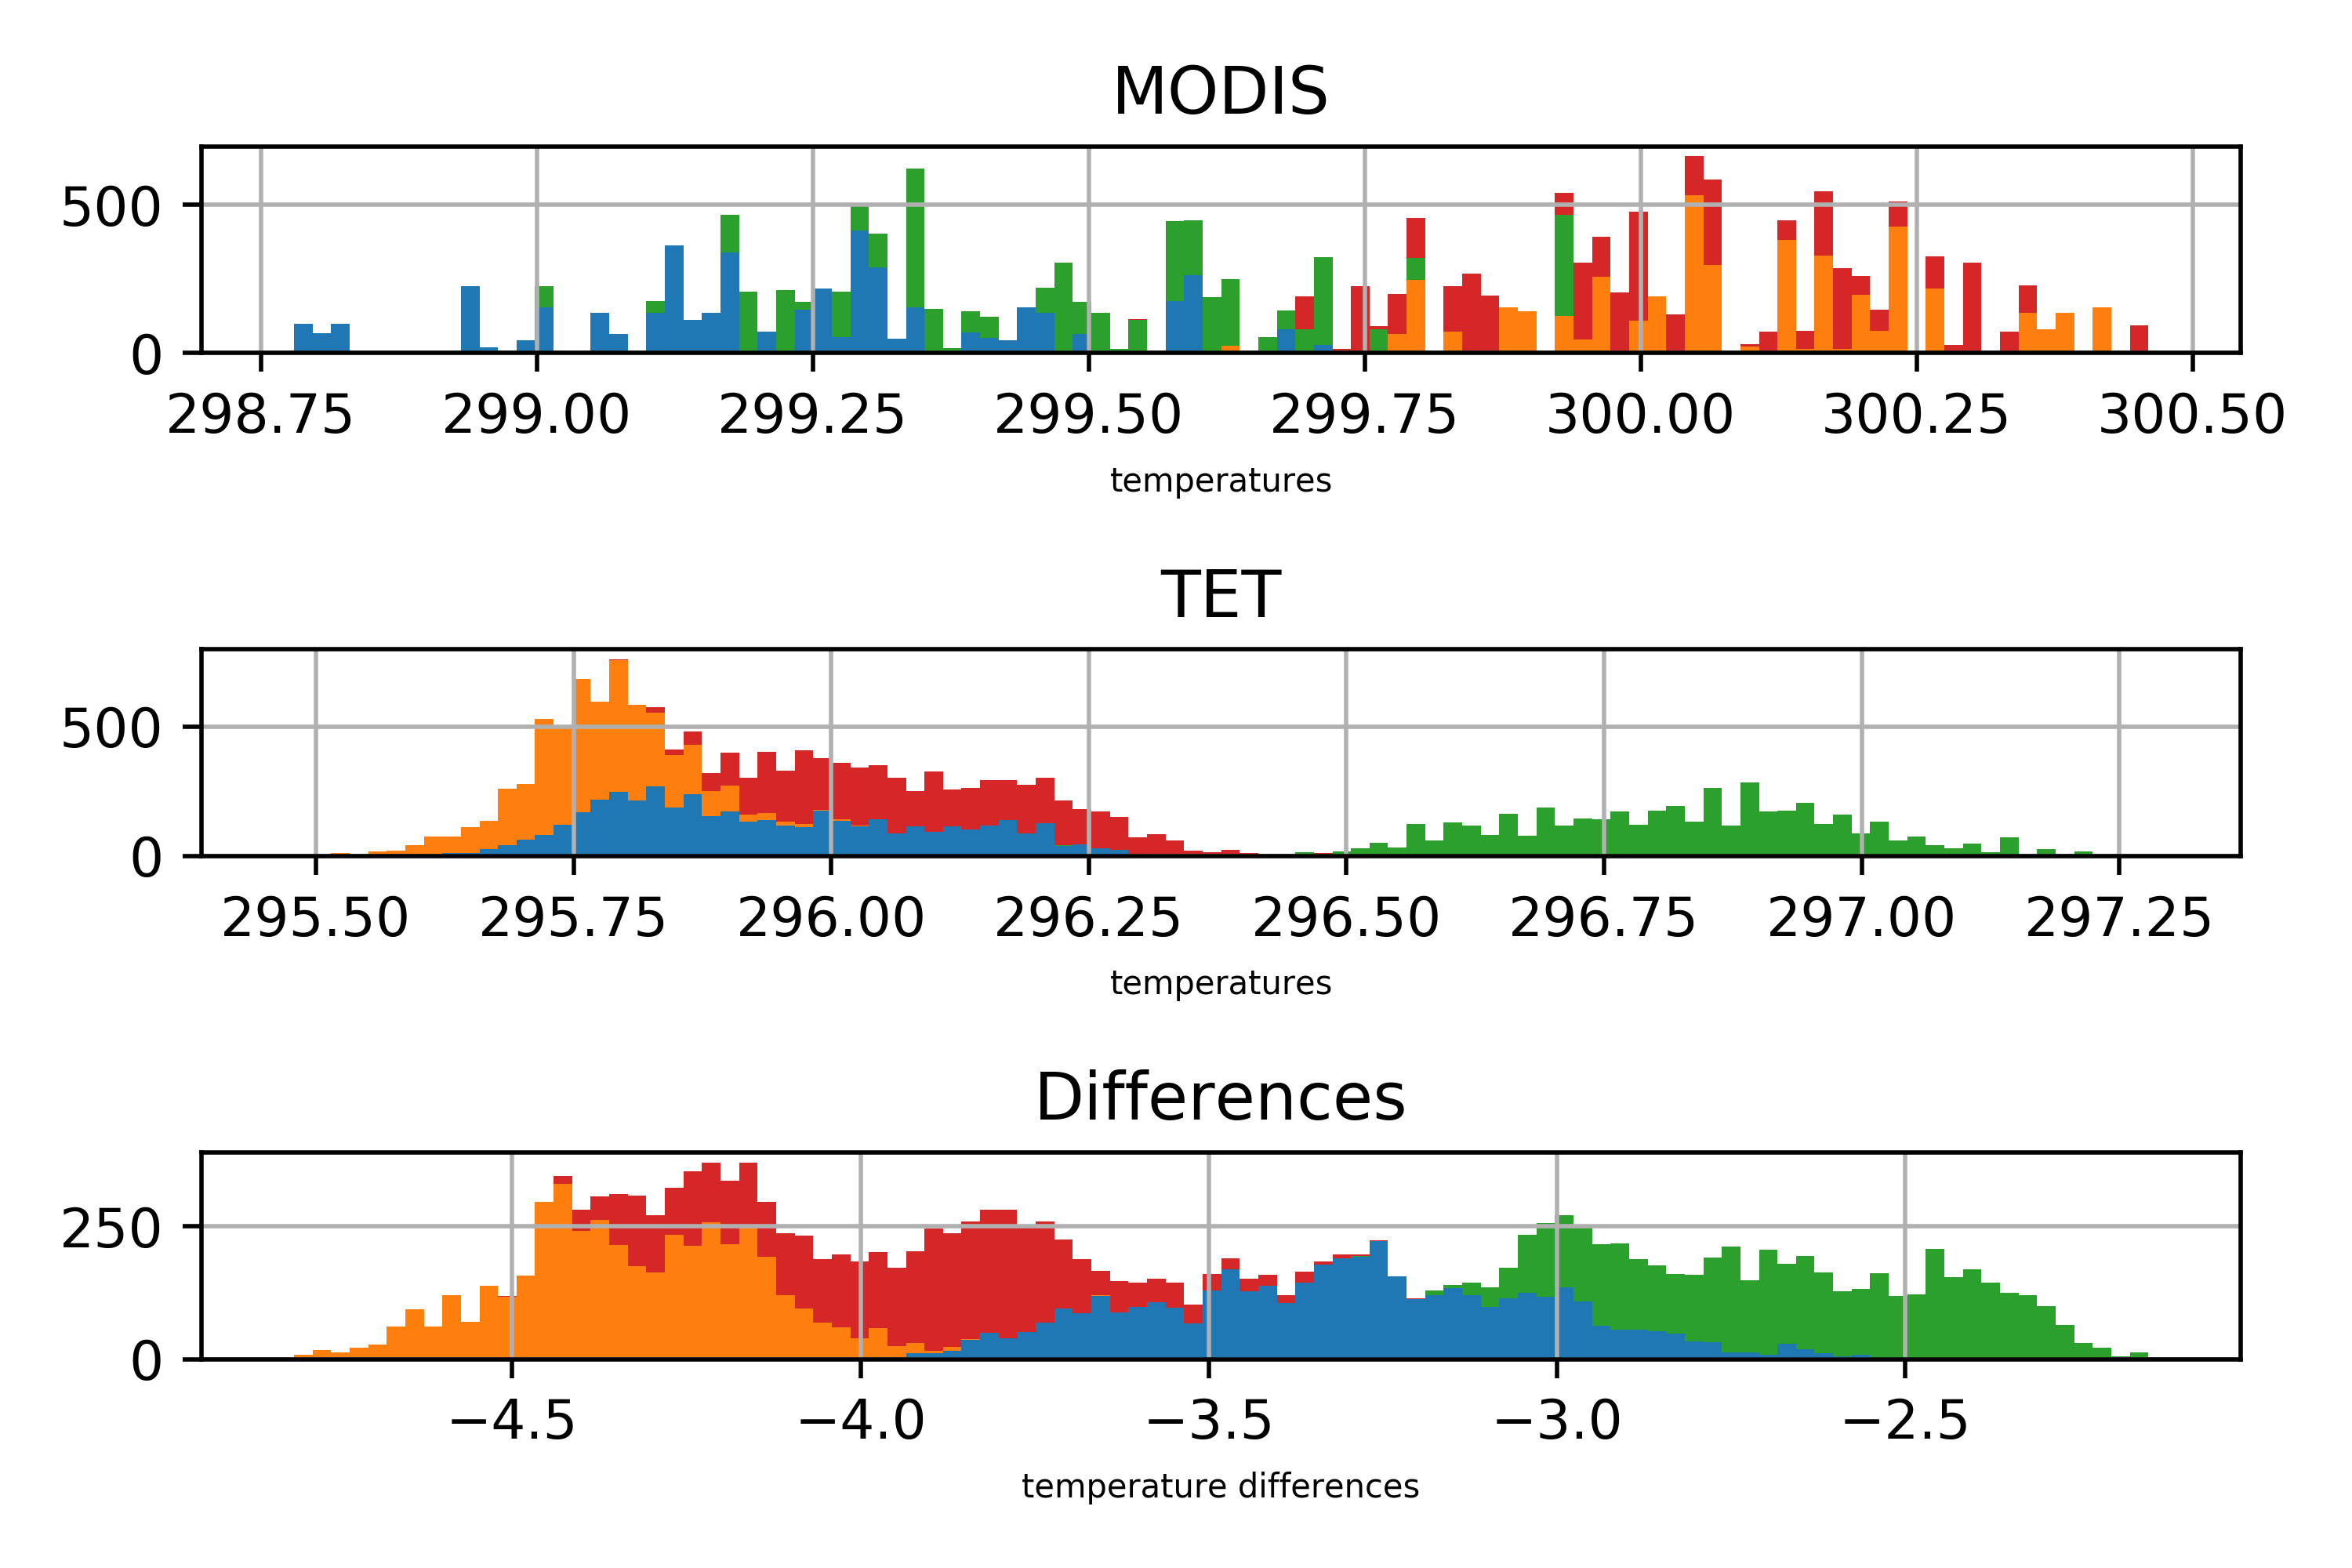
\includegraphics[width = 1.0\textwidth]{rect_all.png}
\caption{Histograms of all sub-areas of MODIS SST and TET-1 MIR band imageries with all the five scale factors. The red solid line in each histogram denotes the mean value and the red dashed line the standard deviation.}
\label{fig:rect_all_sc_all}
\end{figure}

\noindent Afterwards, in order to find the best scale factors for TET-1 MIR and TIR band imageries respectively, a time-serise analysis is performed. The results are shown in Figure \ref{fig:etna_sc_mir_tir}. The Figure \ref{fig:etna_bsc_tem} shows the best scale factor for each Etna scenes (the red solid line) and its corresponding temperature differences (the blue dashed line), which is also the minimal temperature differences. The ideal scale factor will be a constant over time, meaning constant scale factors can be applied to TET-1 MIR and TIR band imageries respectively, or it should be a periodic function of time. However, because of the unstable performance of the sensors, the influence of the space environment, the weather condition and so on, the temperature differences' behaviors of both TET-1 MIR and TIR band imageries are actually random. But it is still clear that for the TET-1 TIR band imagery, the scale factor 1.05 achieves the best performance that the temperature differences resulted from it are most close to zero. The Figure \ref{fig:etna_bsc_tir} also proves that showing that most of the TET-1 TIR band imageries has the best scale factor 1.05.\\

\noindent The situation for the TET-1 MIR band imagery is a bit complicated because the scale factor 1.10 and 1.15 have similar performances. Here scale factor 1.15 are selected artificially because of two points. On one hand, several scenes requires a scale factor higher than 1.15, namely 1.20. On the other hand, as we will present later, scale factor 1.15 shows a better transferability and performs better for scenes of other sites.\\

\begin{figure}[!htbp]
\centering
\subfigure[MIR band]{
\label{fig:etna_sc_mir}
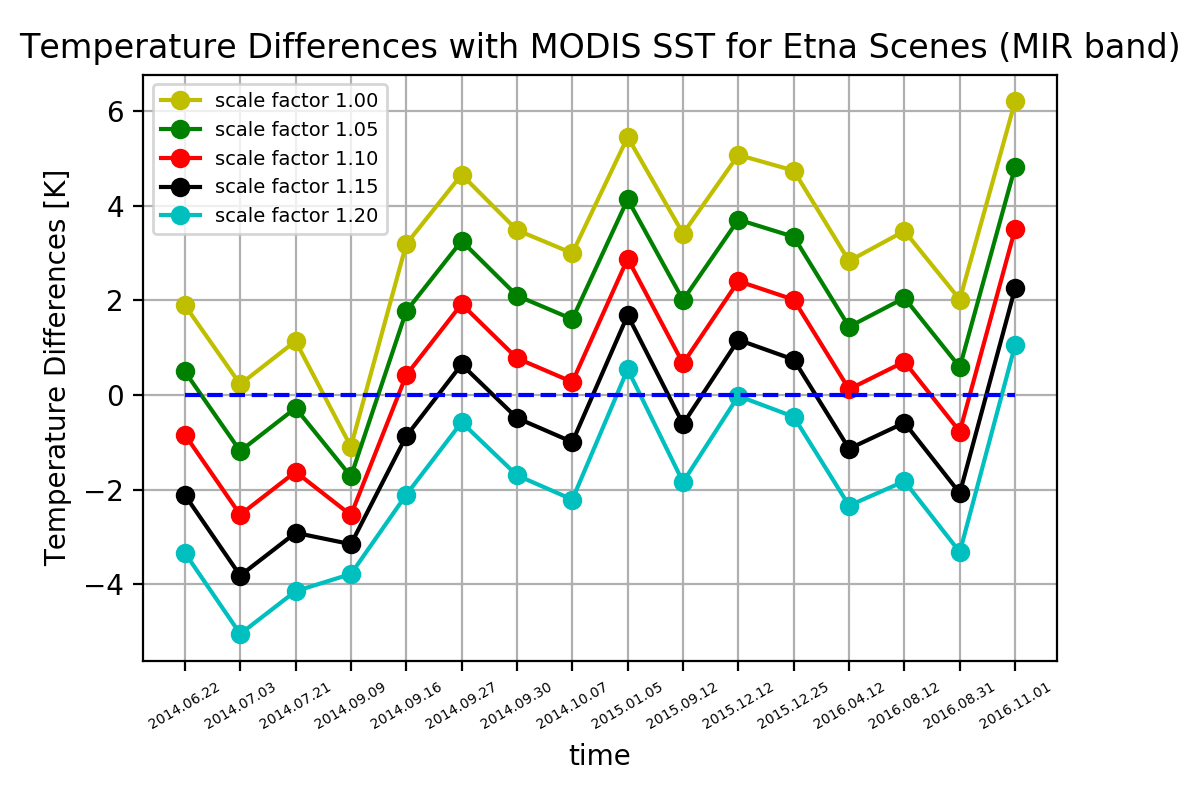
\includegraphics[width = 0.8\linewidth]{Etna_scf_mir.png}}
\hspace{0.5in}
\subfigure[TIR band]{
\label{fig:etna_sc_tir}
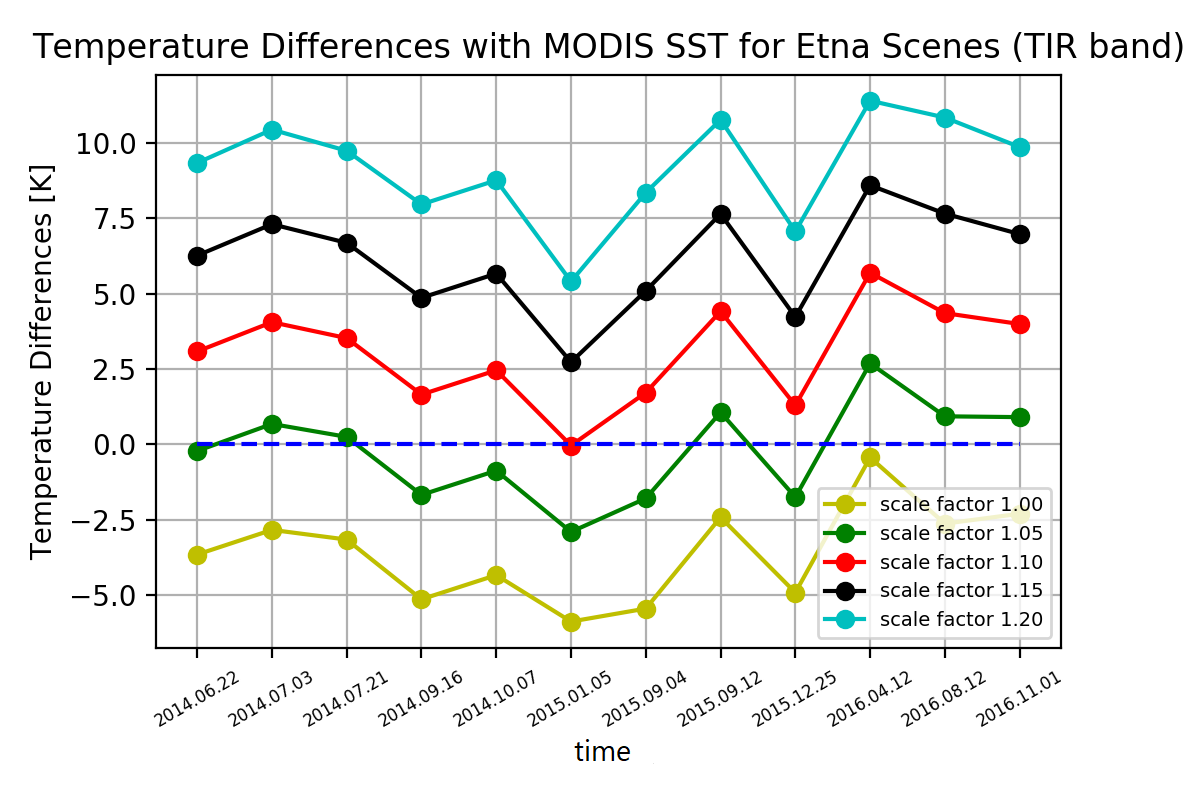
\includegraphics[width = 0.8\linewidth]{Etna_scf_tir.png}}
\caption{Temperature differences between TET-1 surface temperature maps and MODIS SST (Etna).}
\label{fig:etna_sc_mir_tir}
\end{figure}

\begin{figure}[!htbp]
\centering
\subfigure[MIR band]{
\label{fig:etna_bsc_mir}
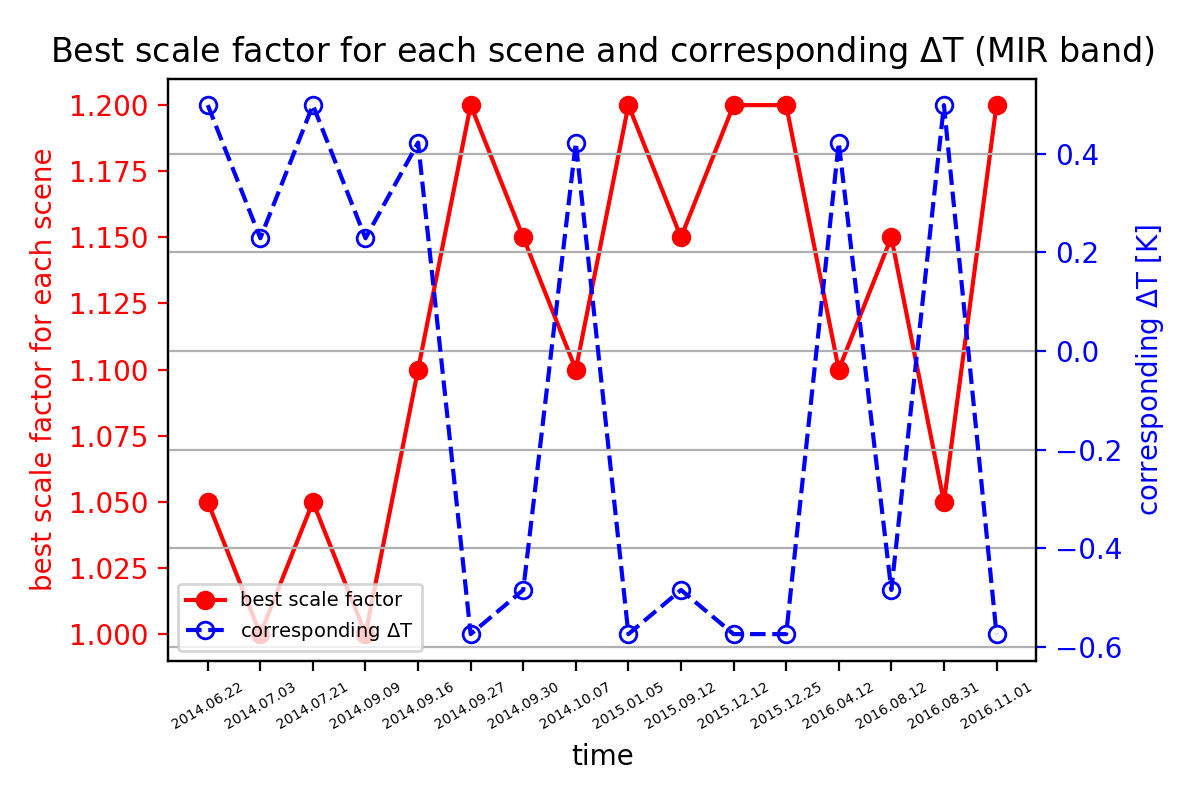
\includegraphics[width = 0.8\linewidth]{Etna_bsc&tem_mir.png}}
\hspace{0.5in}
\subfigure[TIR band]{
\label{fig:etna_bsc_tir}
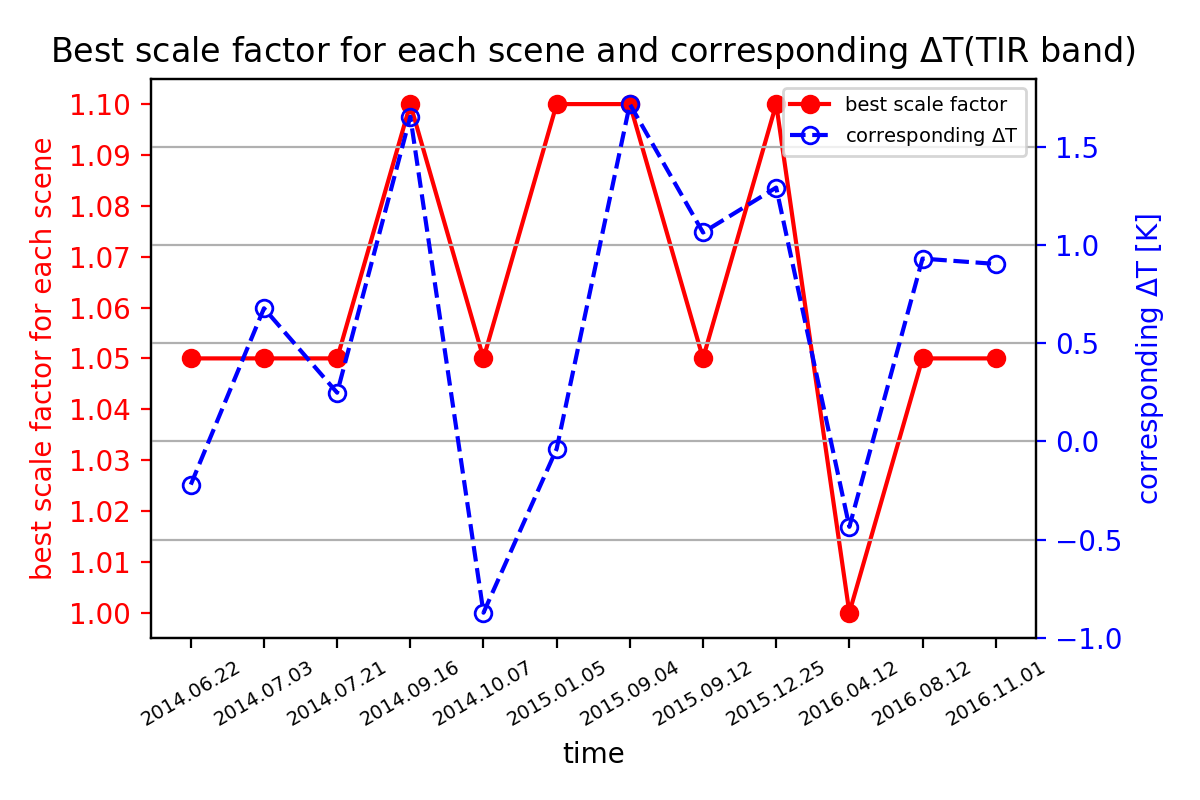
\includegraphics[width = 0.8\linewidth]{Etna_bsc&tem_tir.png}}
\caption{The best scale factors for each Etna scenes and its corresponding temperature differences. The red solid line is the best scale factor for each Etna scene. The blue dashed line is the minimal temperature differences resulted from that scale factor.}
\label{fig:etna_bsc_tem}
\end{figure}

\noindent As shown in Figure \ref{fig:etna_bsc&temComp}(a) that the temperature differences between MODIS SST and the surface temperature map in MIR band resulted from scale factor 1.15 are at most 4 K higher than the minimal temperature differences and at most of the time they differ only between 1 to 2 K. For surface temperature map in TIR band results from scale factor 1.05 differ from the smallest temperature differences at most 4 K as well.\\

\begin{figure}[!htbp]
\centering
\subfigure[MIR band]{
\label{fig:etna_bsc&temComp_mir}
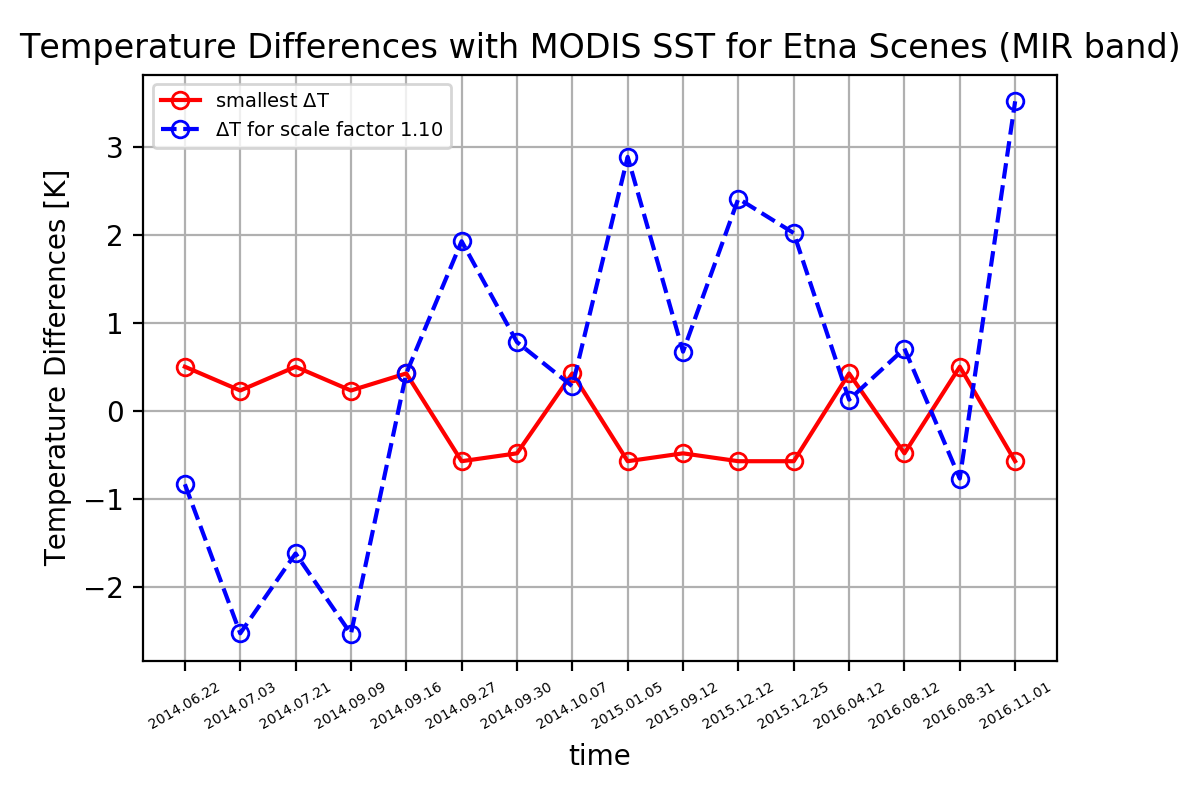
\includegraphics[width = 0.8\linewidth]{Etna_bsc&temCom_mir.png}}
\hspace{0.5in}
\subfigure[TIR band]{
\label{fig:etna_bsc&temComp_tir}
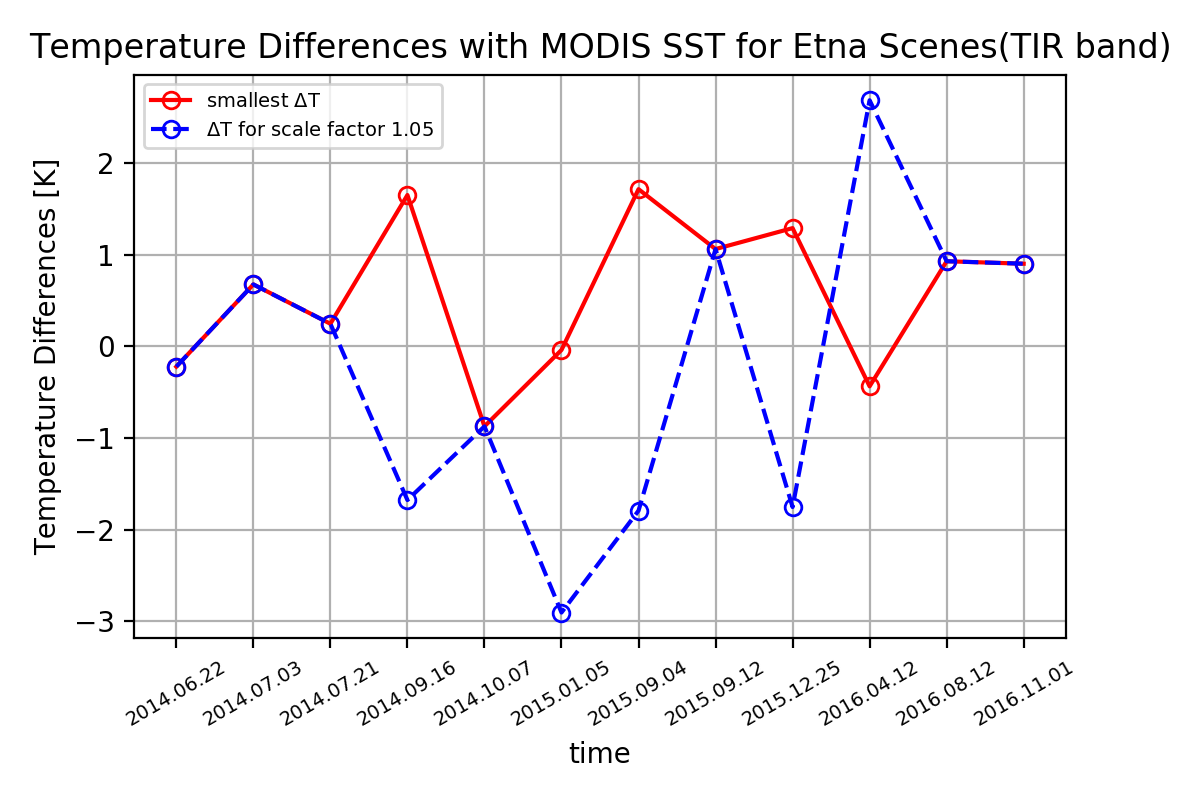
\includegraphics[width = 0.8\linewidth]{Etna_bsc&temCom_tir.png}}
\caption{The minimal temperature differences and the temperature differences resulted from scale factor 1.15 and scale factor 1.05. The red solid line is the minimal temperature differences for each Etna scene. The blue dashed line is the temperature differences resulted from the selected scale factors for MIR and TIR band imageries, scale factor 1.15 (upper) and scale factor 1.05 (lower), respectively.}
\label{fig:etna_bsc&temComp}
\end{figure}

%-----------------------------------
%	SUBSECTION 3
%-----------------------------------

% \subsection{Calibrations}

%-----------------------------------
%	SUBSECTION 3
%-----------------------------------
\subsection{transferability test (SST)}
The best scale factors for the TET-1 MIR and TIR band imageries are selected as 1.15 and 1.05 respectively in the previous section. But they are selected based on TET-1 imageries of one site only. Before applying them to other imageries, their transferability should be tested to see whether the scale factors got from Etna scenes are suitable for other sites as well. Consequently, three other scenes of Etna, one scene of Portugal and two scenes of Demmin are used as test scenes to validate the chosen scale factors.\\

\begin{figure}[!htbp]
\centering
\subfigure[Portugal]{
\label{fig:Portugal}
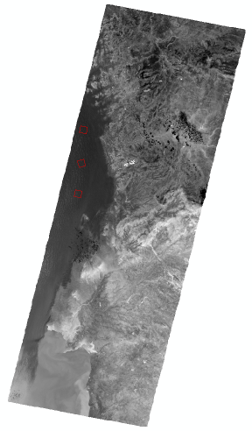
\includegraphics[width = 0.4\linewidth]{Portugal.png}}
\vspace{0.5in}
\subfigure[Demmin]{
\label{fig:Demmin}
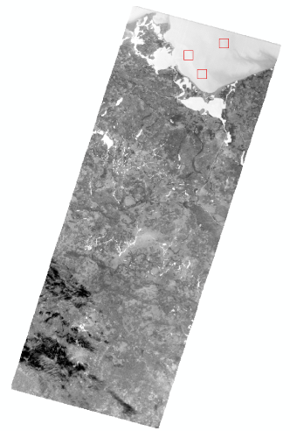
\includegraphics[width = 0.4\linewidth]{Demmin.png}}
\caption{The example figures of Portugal and Demmin. The red rectangles represent the selected sub-areas.}
\label{fig:portugal&demmin}
\end{figure}

\noindent Besides the chosen scale factor 1.15 for MIR band imagery and 1.05 for TIR band imagery, the performances of scale factor 1.10 and 1.20 are also presented for the MIR band imagery as comparison and for TIR band imagery, the performances of scale factor 1.00 and 1.10 are displayed as well for the same purpose. As shown in Figure \ref{fig:SST_test}, scale factor 1.15 for MIR band imagery and scale factor 1.05 for TIR band imagery are not always optimal scale factors for each scene, however, they demonstrate better performances than the other scale factors over time and sites.\\

\begin{figure}[!htbp]
\centering
\subfigure[MIR band]{
\label{fig:SST_test_mir}
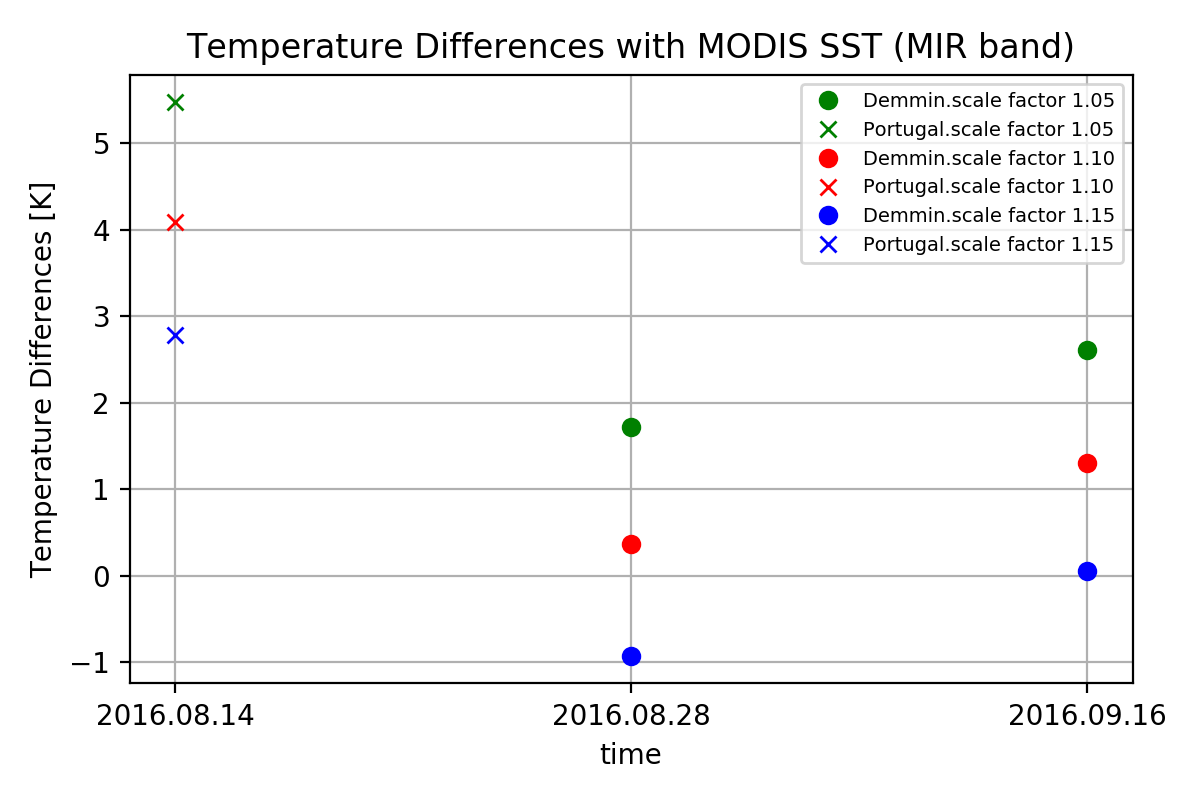
\includegraphics[width = 0.8\linewidth]{sst_test&comp_mir.png}}
\hspace{0.5in}
\subfigure[TIR band]{
\label{fig:SST_test_tir}
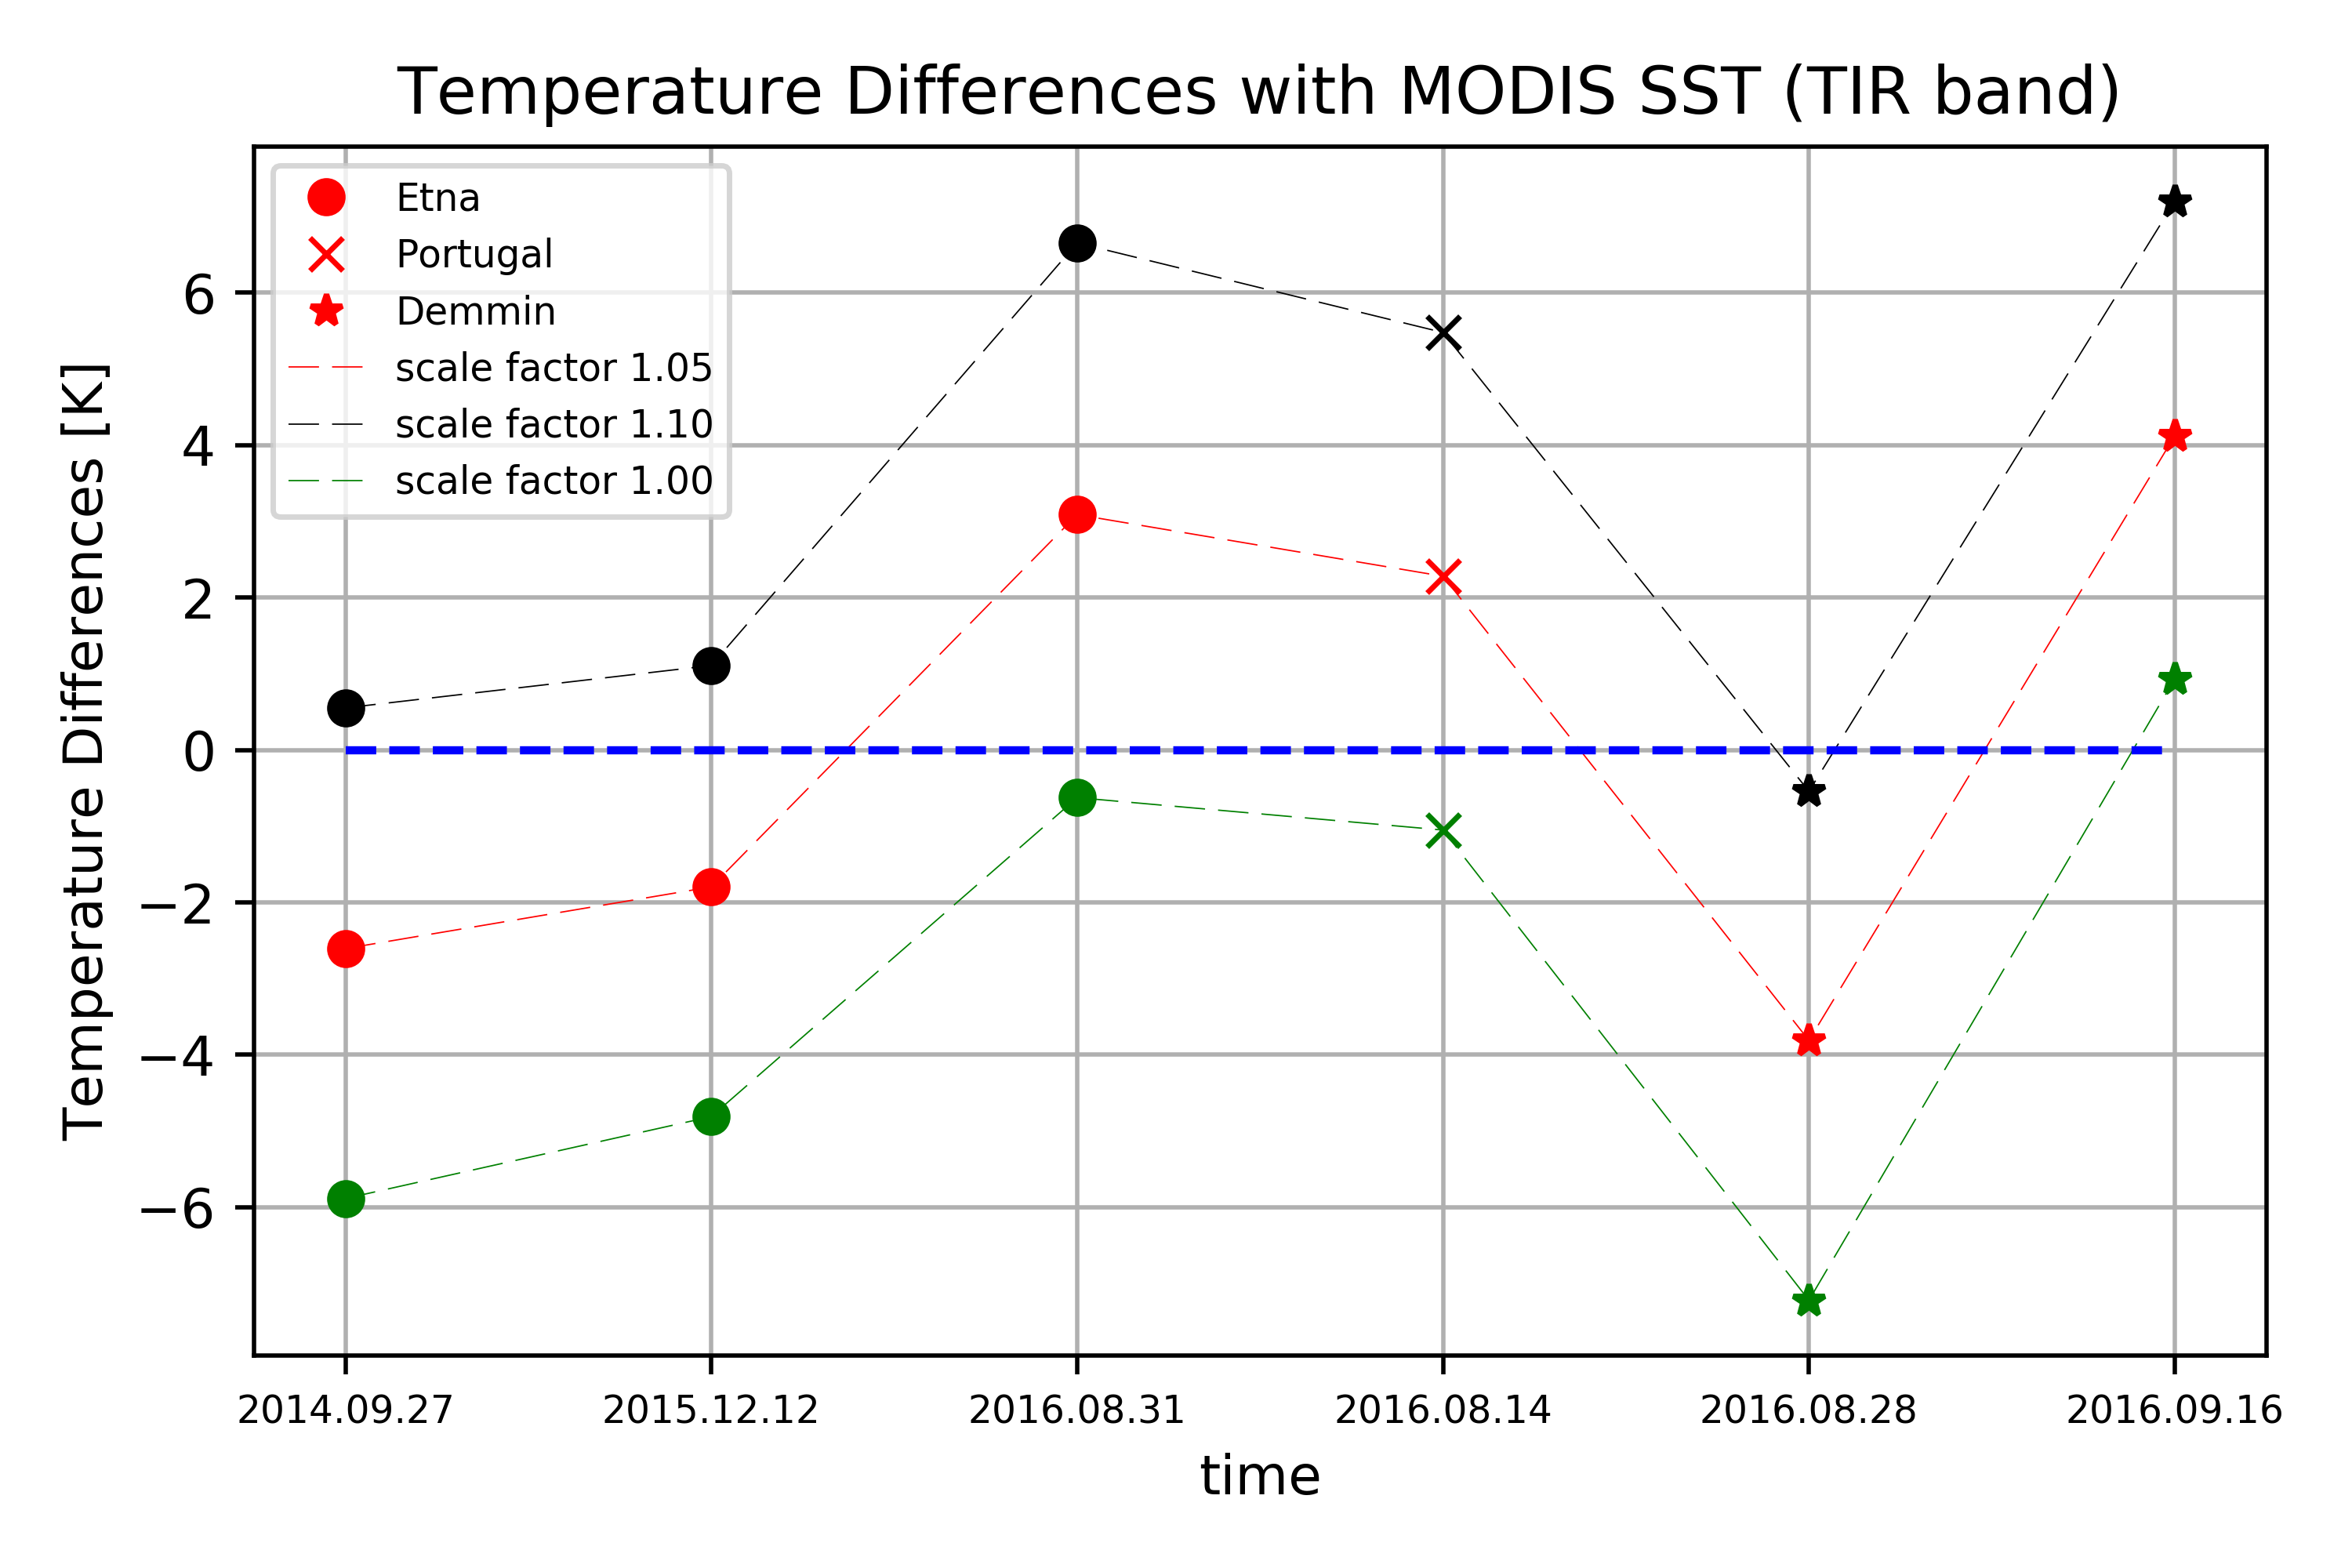
\includegraphics[width = 0.8\linewidth]{sst_test&comp_tir.png}}
\caption{Transferability test: temperature differences between TET-1 surface temperature maps and MODIS SST.}
\label{fig:SST_test}
\end{figure}

%-----------------------------------
%	SUBSECTION 4
%-----------------------------------

\subsection{Results comparison with MODIS LST and calibration}
The similar comparison is done between the temperature results from MITIP and MODIS LST over the scenes of the test site Libya-1. However, the emissivities of different land features vary a lot. So the problem that which band of the emissivity maps to be used matters. The temperature maps of MITIP resulted from different emissivity maps are presented as follows.\\

\begin{figure}[!htbp]
\centering
\subfigure[Temperature (Libya-1) with different emissivities]{
\label{fig:emi_Libya_1}
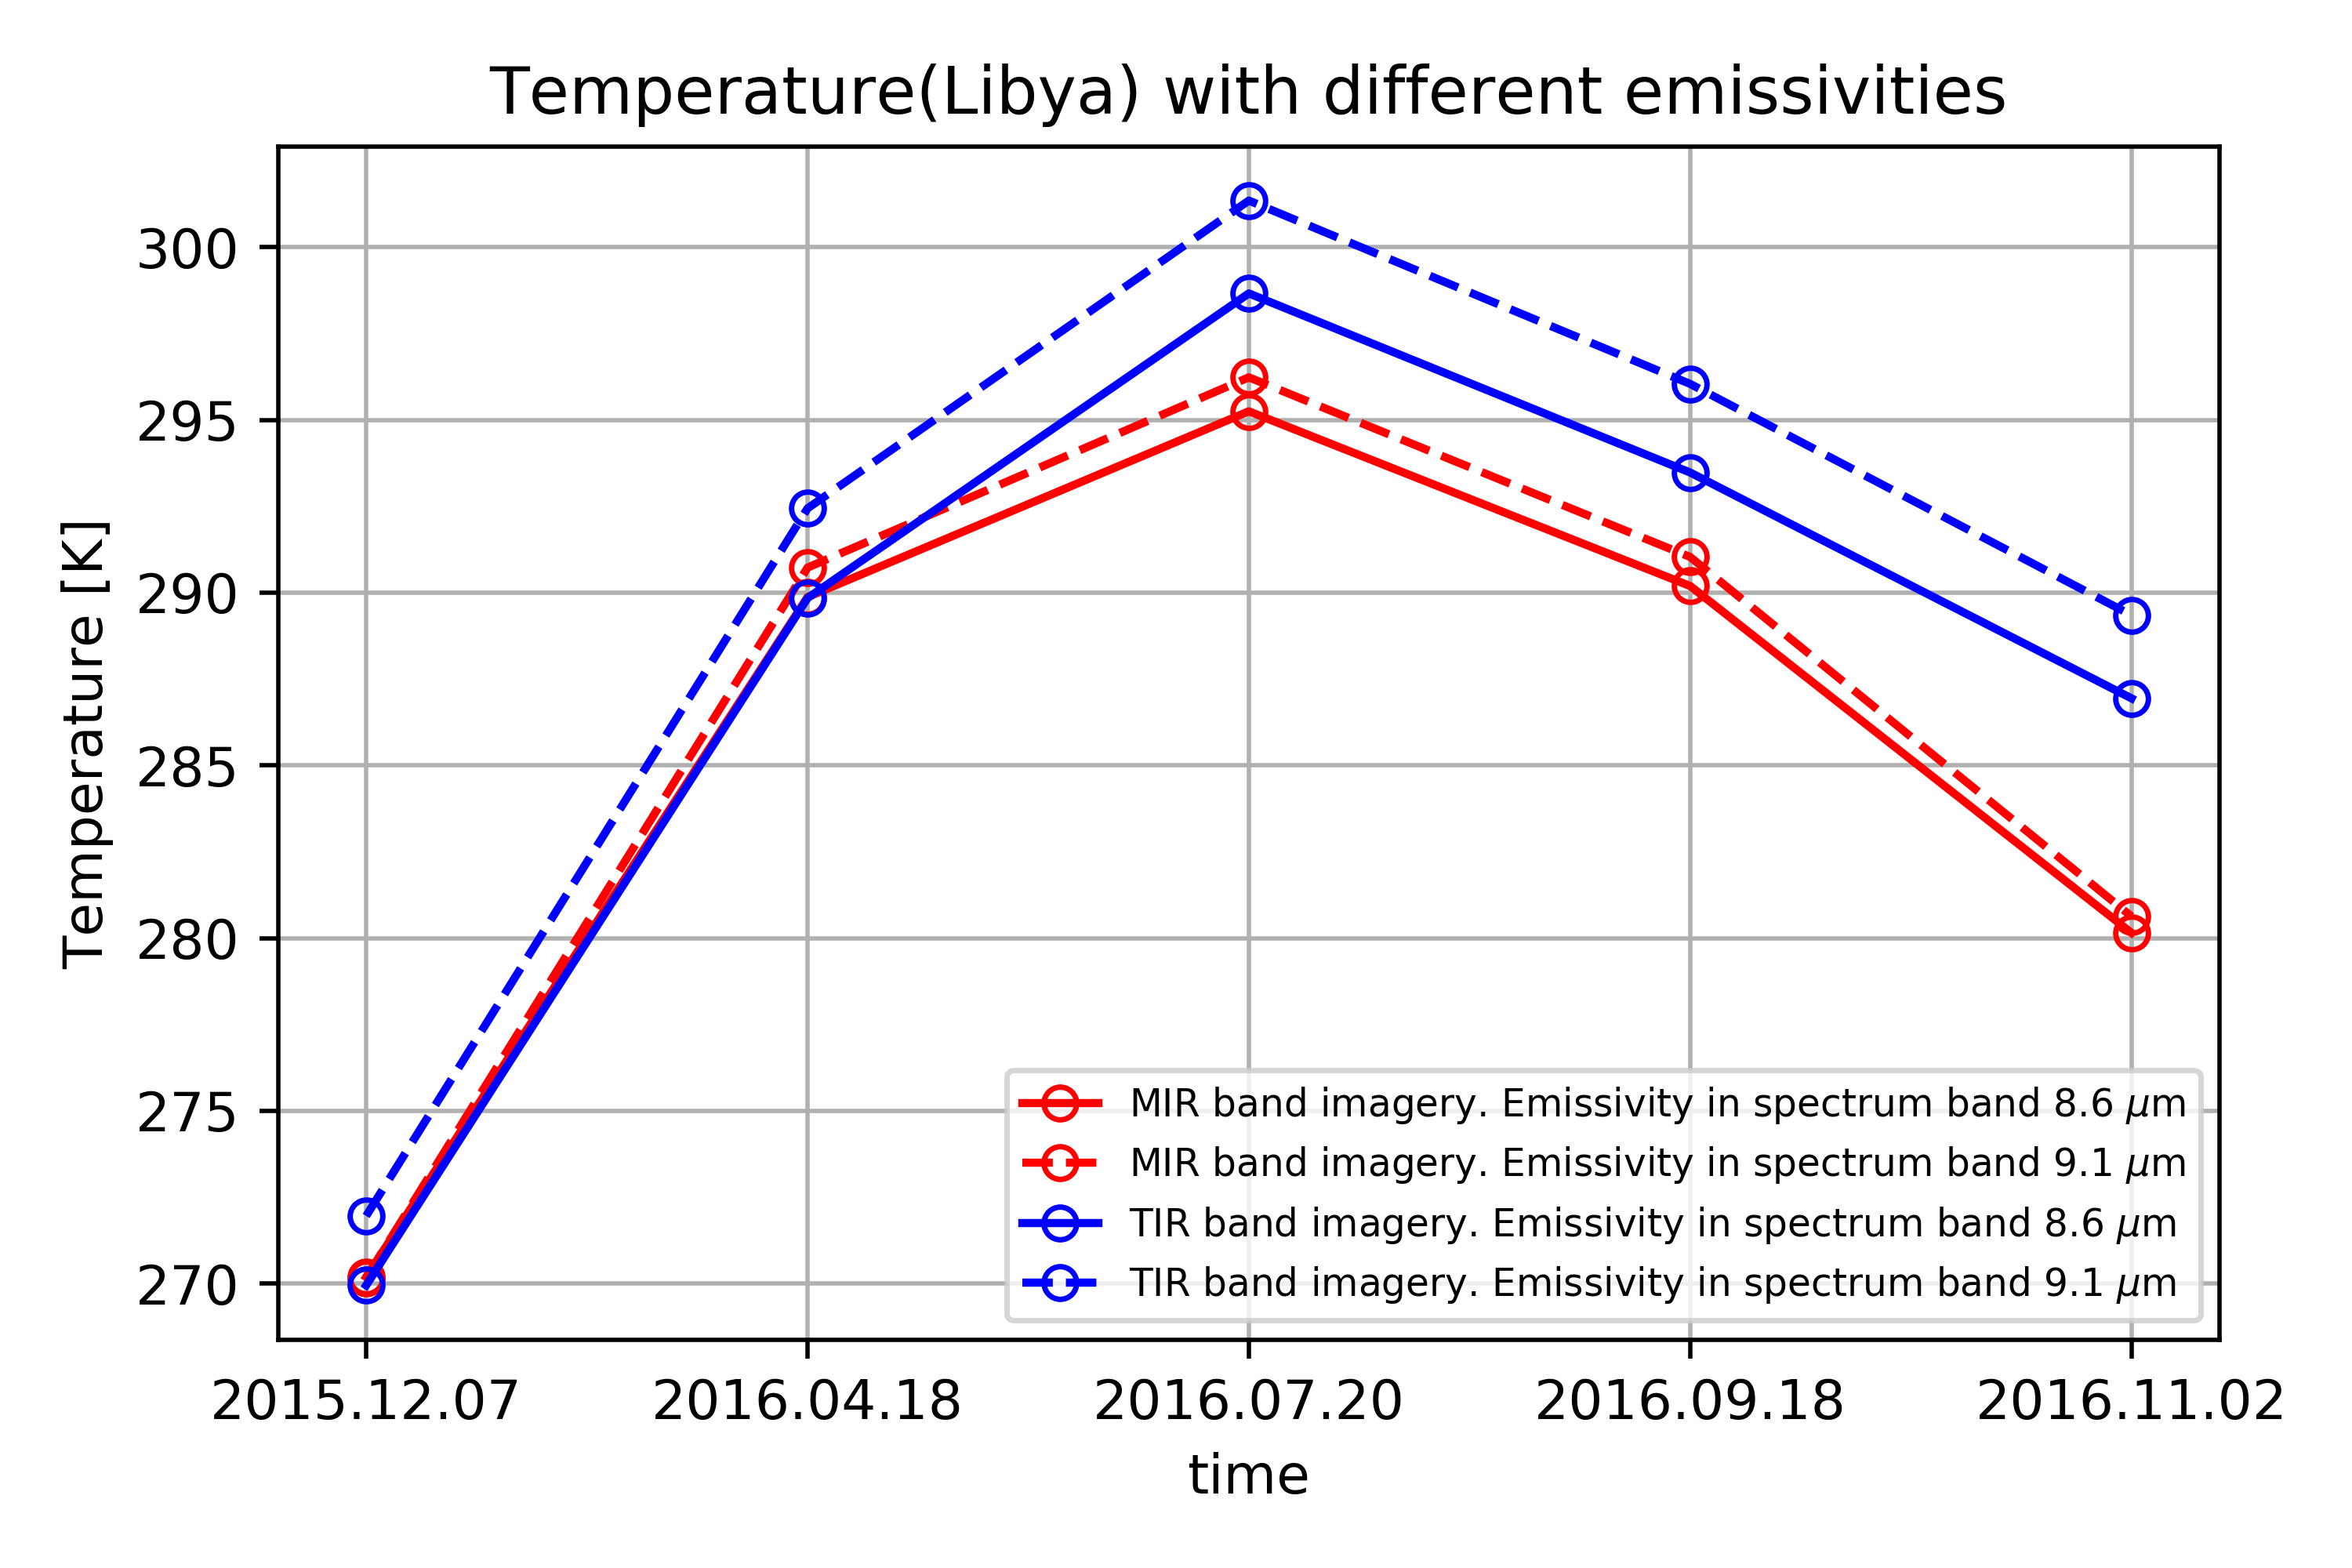
\includegraphics[width = 0.8\linewidth]{diff_emi1_Lybia.png}}
\hspace{0.5in}
\subfigure[Temperature differences (Libya-1) with different emissivities]{
\label{fig:emi_Libya_2}
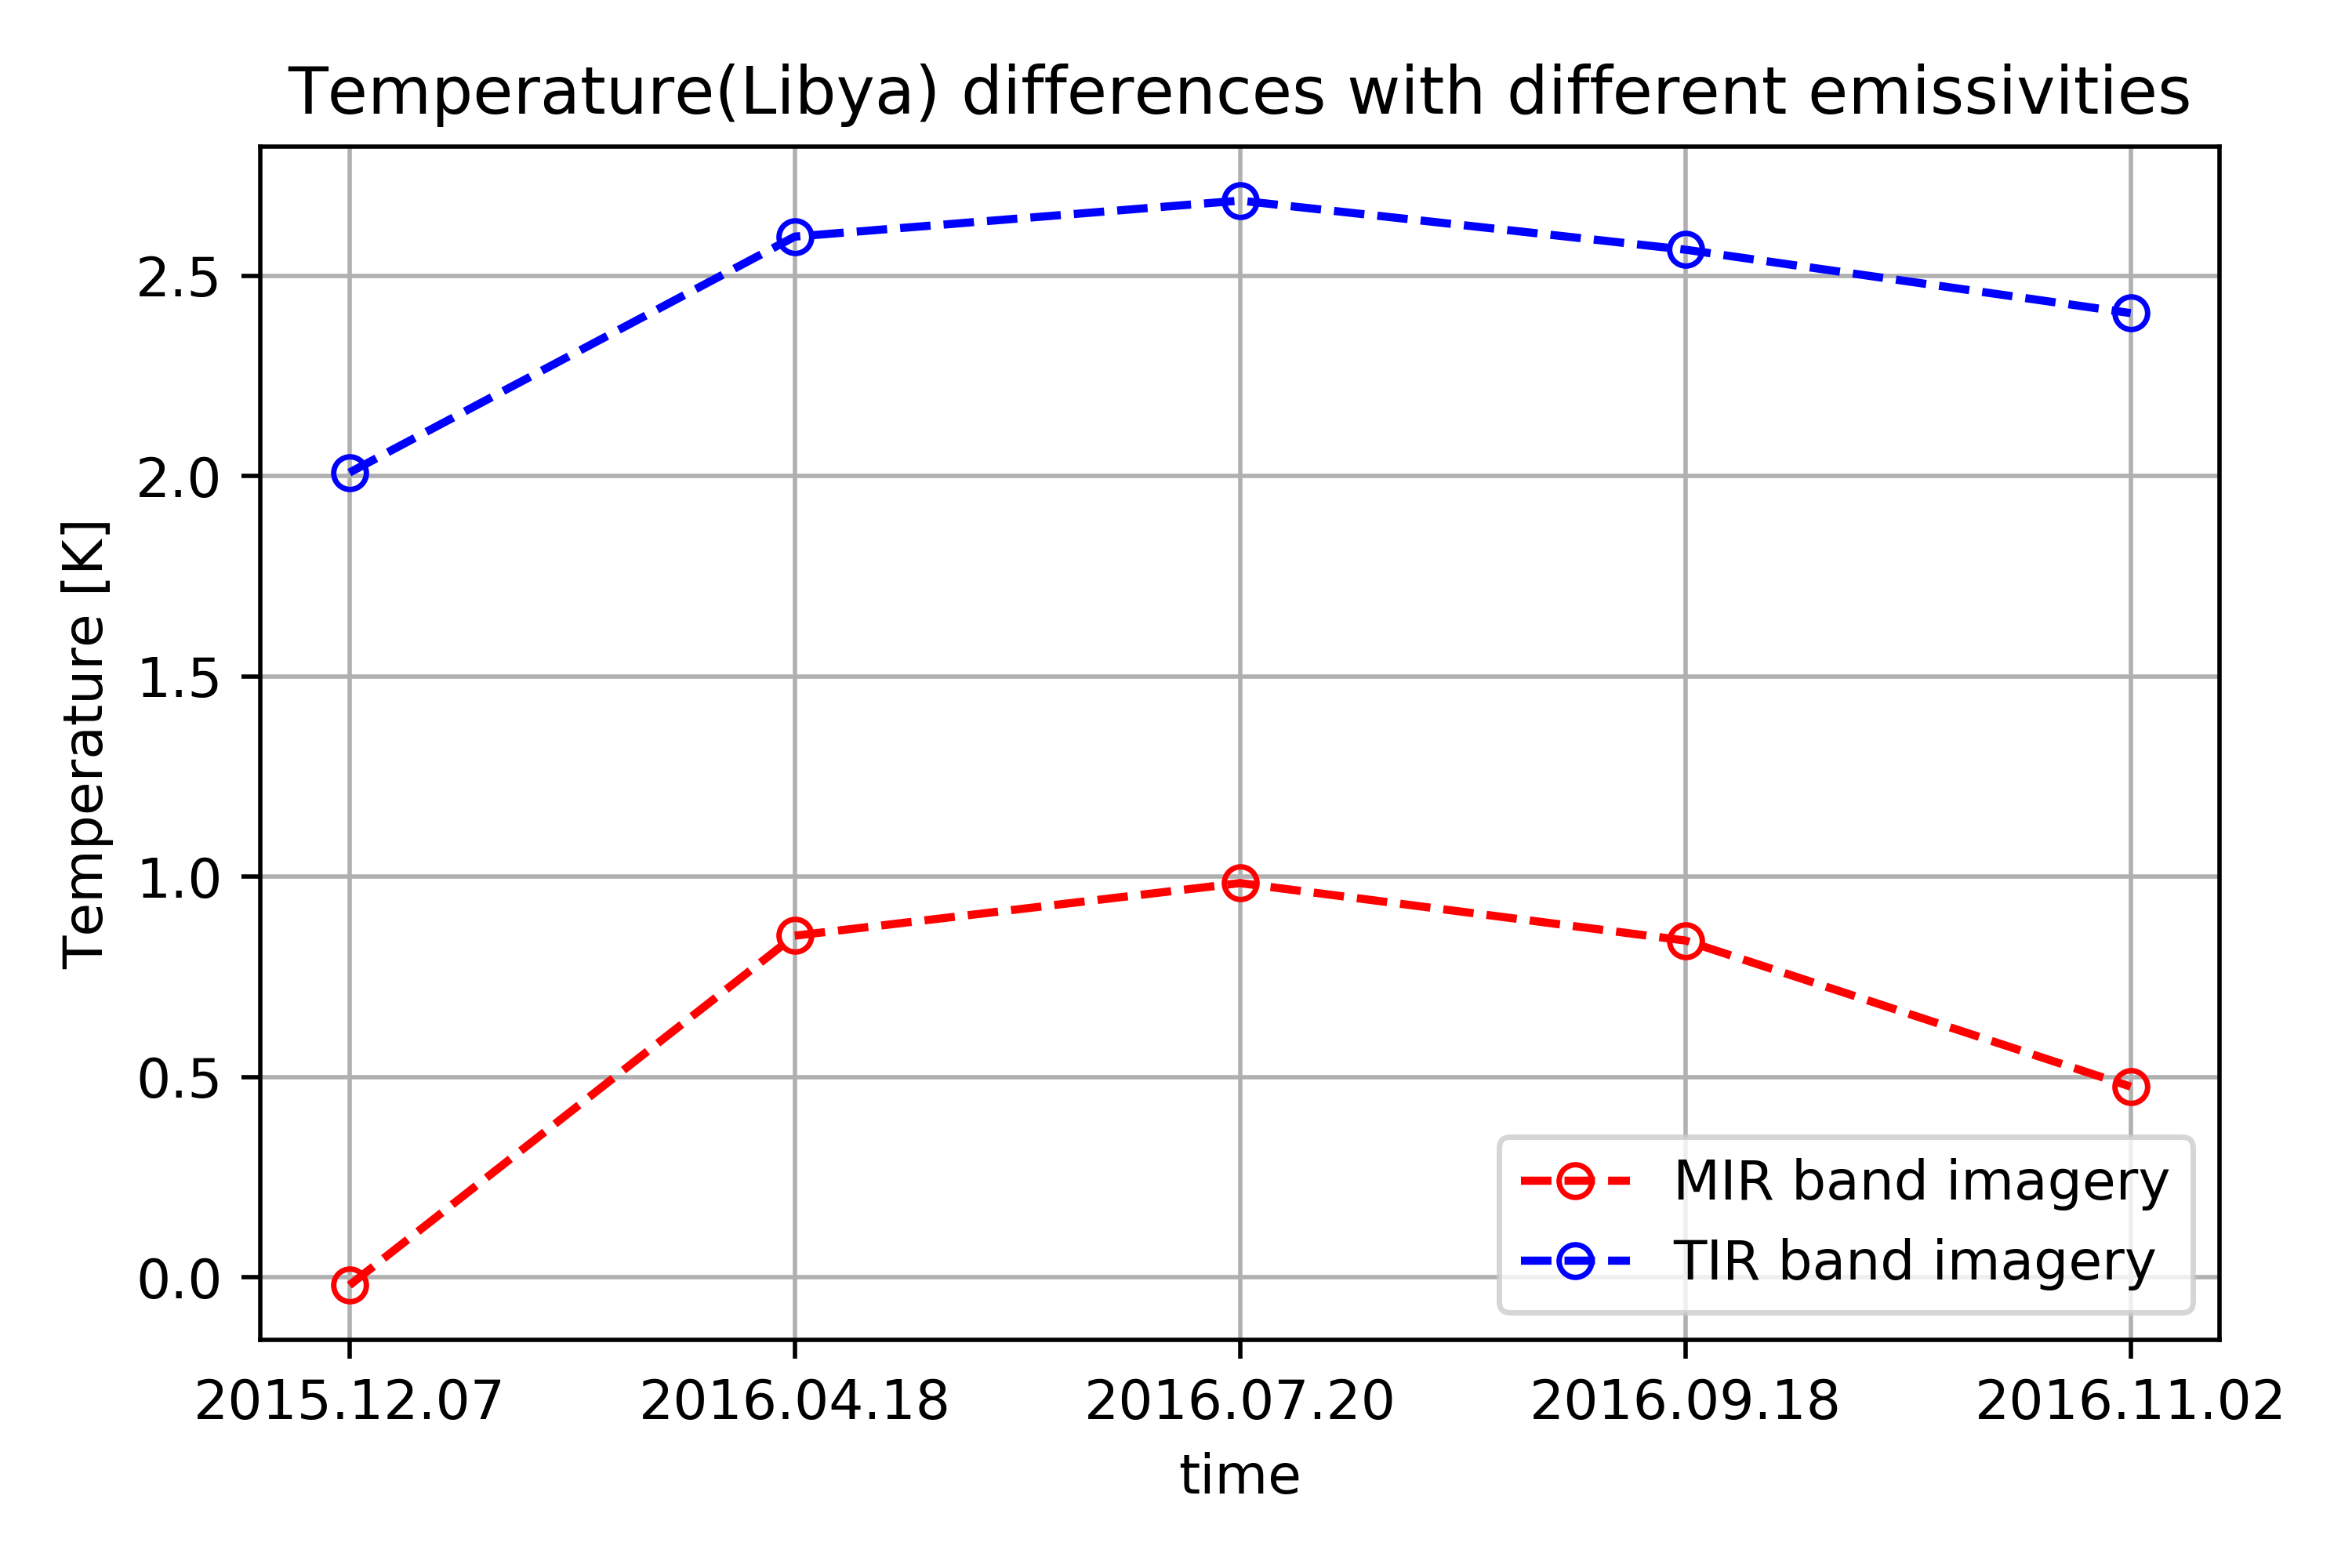
\includegraphics[width = 0.8\linewidth]{diff_emi2_Lybia.png}}
\caption{The effect of different emissivities on the surface temperature maps from MITIP.}
\label{fig:diff_emi_Lybia}
\end{figure}

\noindent from the Figure \ref{fig:diff_emi_Lybia} it is clear that different emissivities maps have great influence on the temperature maps from MITIP.  Figure \ref{fig:emi_Libya_2} shows that the temperature differences in TET-1 TIR band imageries are much higher than the temperature differences in the MIR band imageries both caused by the emissivity maps. Consequently, the focus will be laid on the TET-1 TIR band imageries.\\

\begin{figure}[!htbp]
\centering
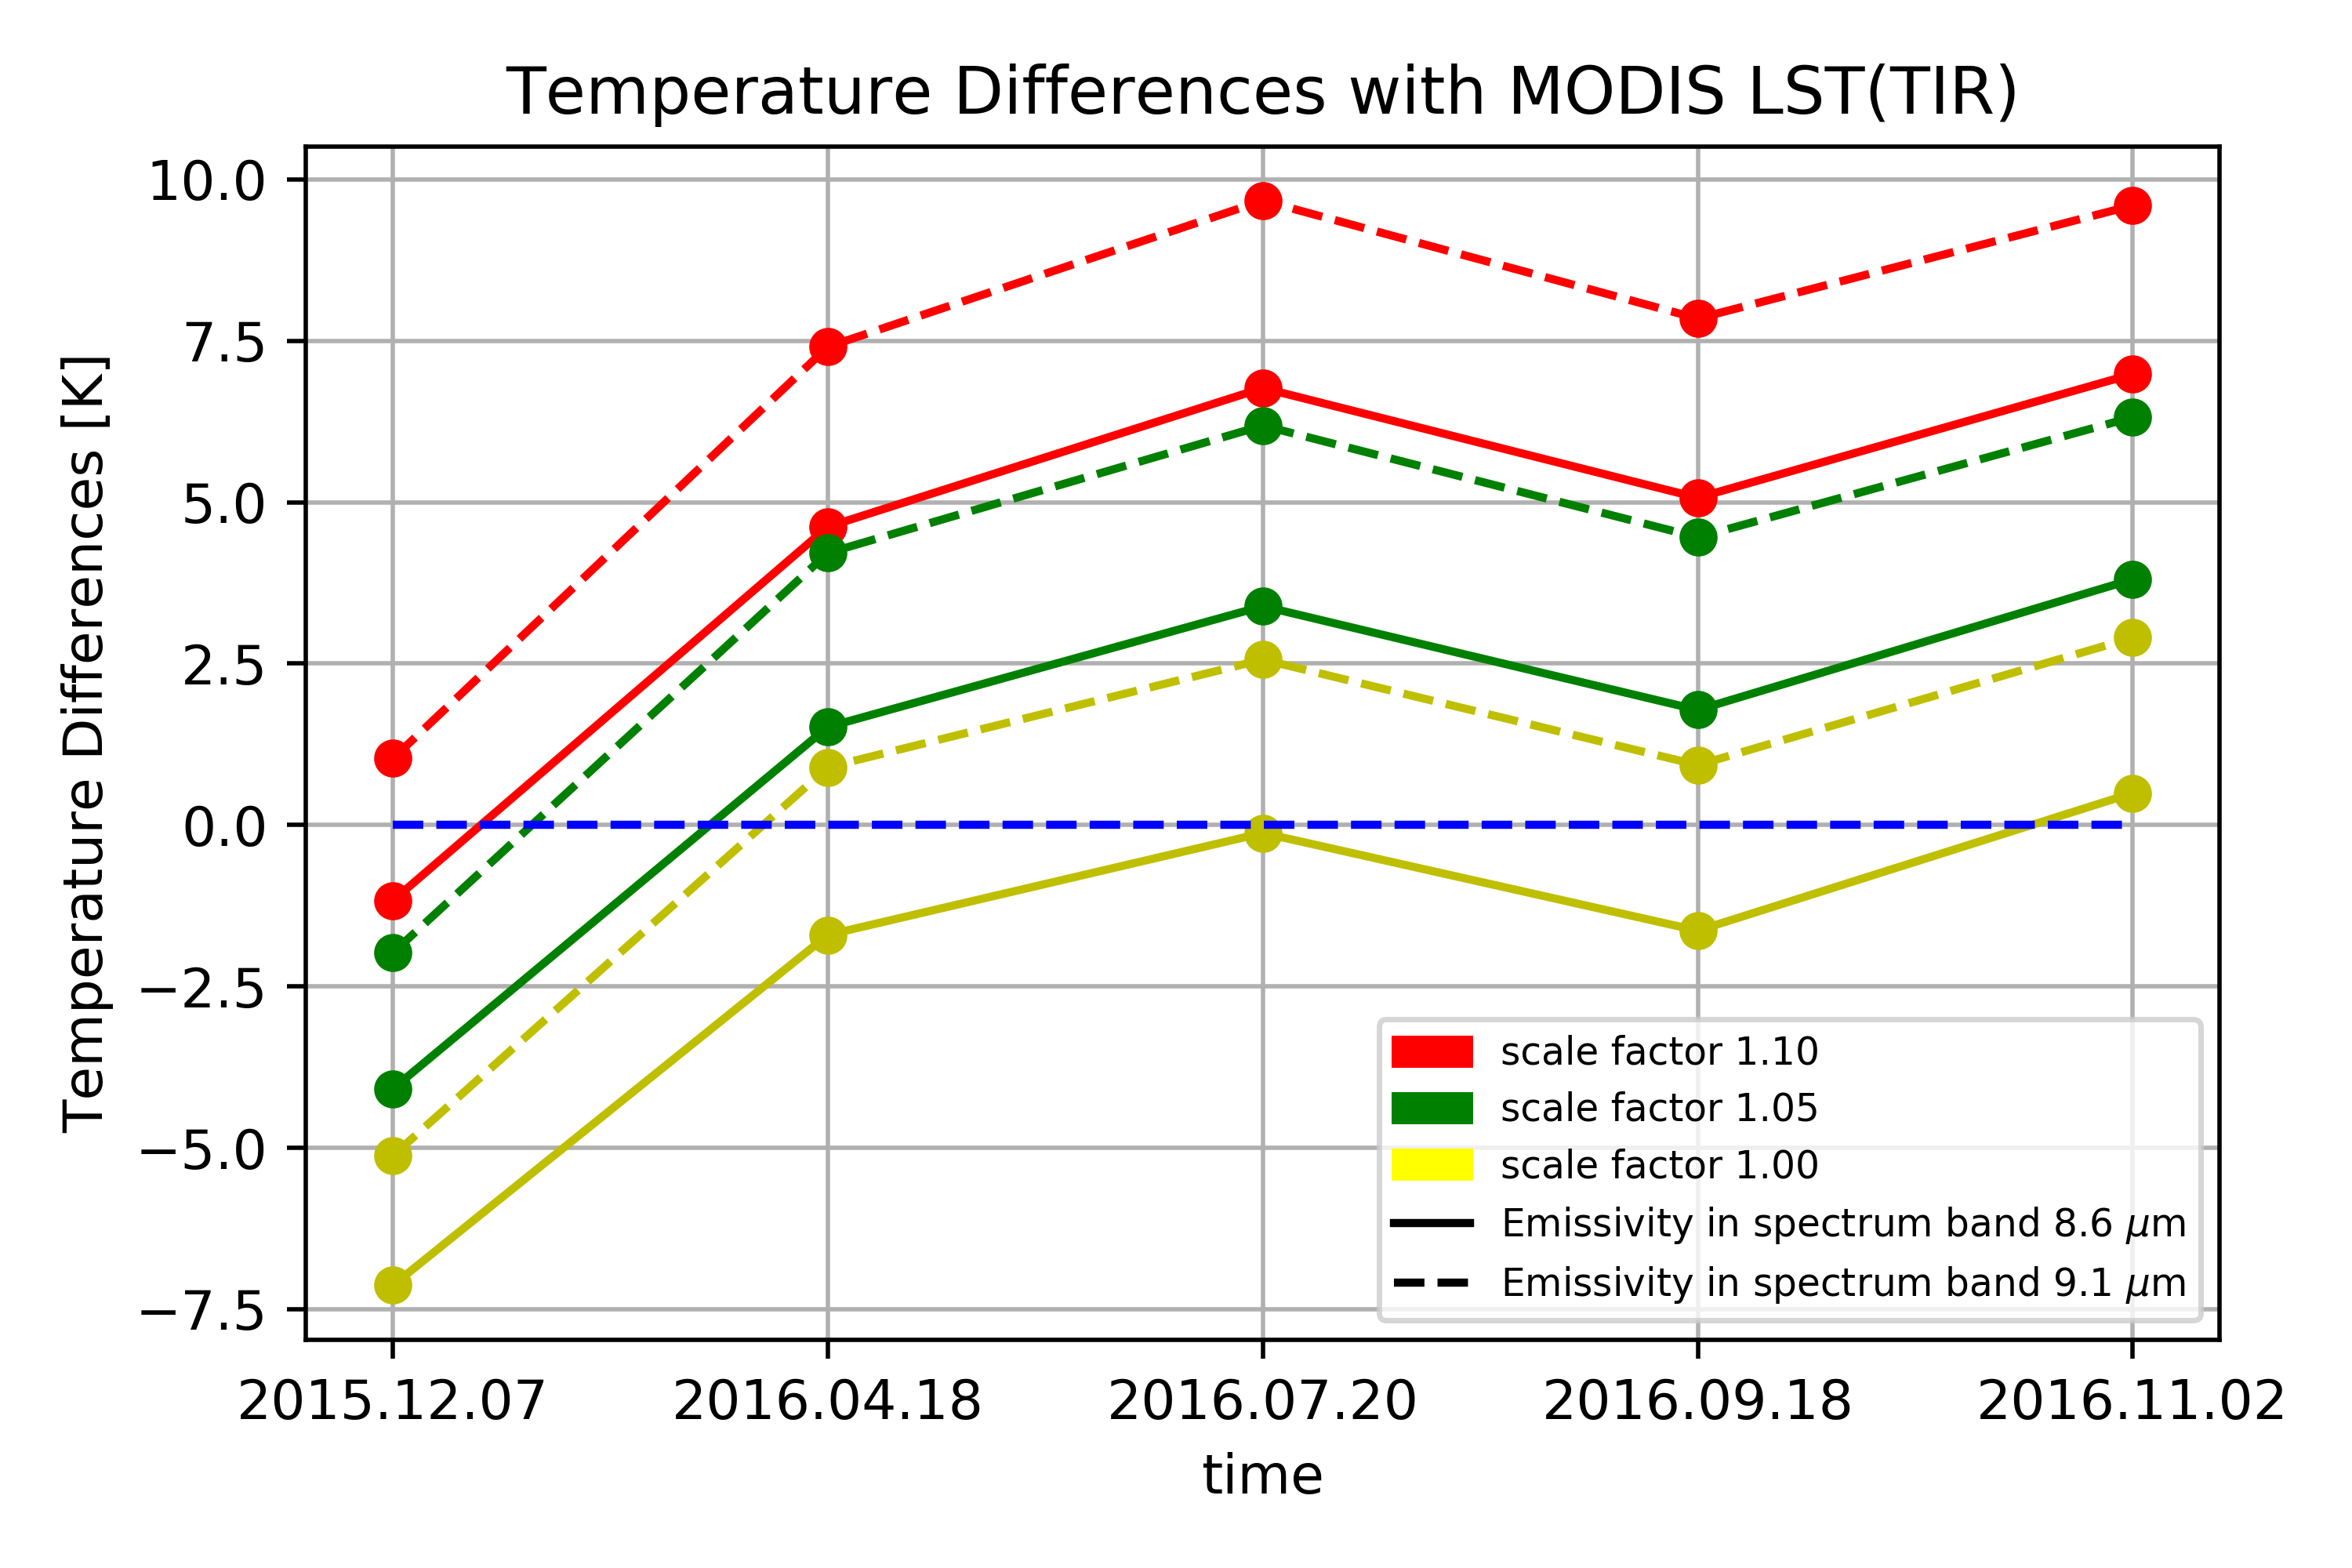
\includegraphics[width = 0.8\textwidth]{diff_emi_tir1.png}
\caption{Temperature differences (Lybia-1) between the surface temperature maps in TIR band and MODIS LST.}
\label{fig:diff_emi_tir1}
\end{figure}

\noindent Figure \ref{fig:diff_emi_tir1} shows that the emissivity maps have effects comparable with the effects of the scale factors and it is clear that with the same scale factor, the temperature differences in TIR band resulted from emissivity map in 8.6 $\mu$m are much lower than these from the emissivity in band 9.1 $\mu$m. The temperature differences in MIR band with different emissivity maps also prove that as shown in Figure \ref{fig:diff_emi_mir1}.\\

\begin{figure}[!htbp]
\centering
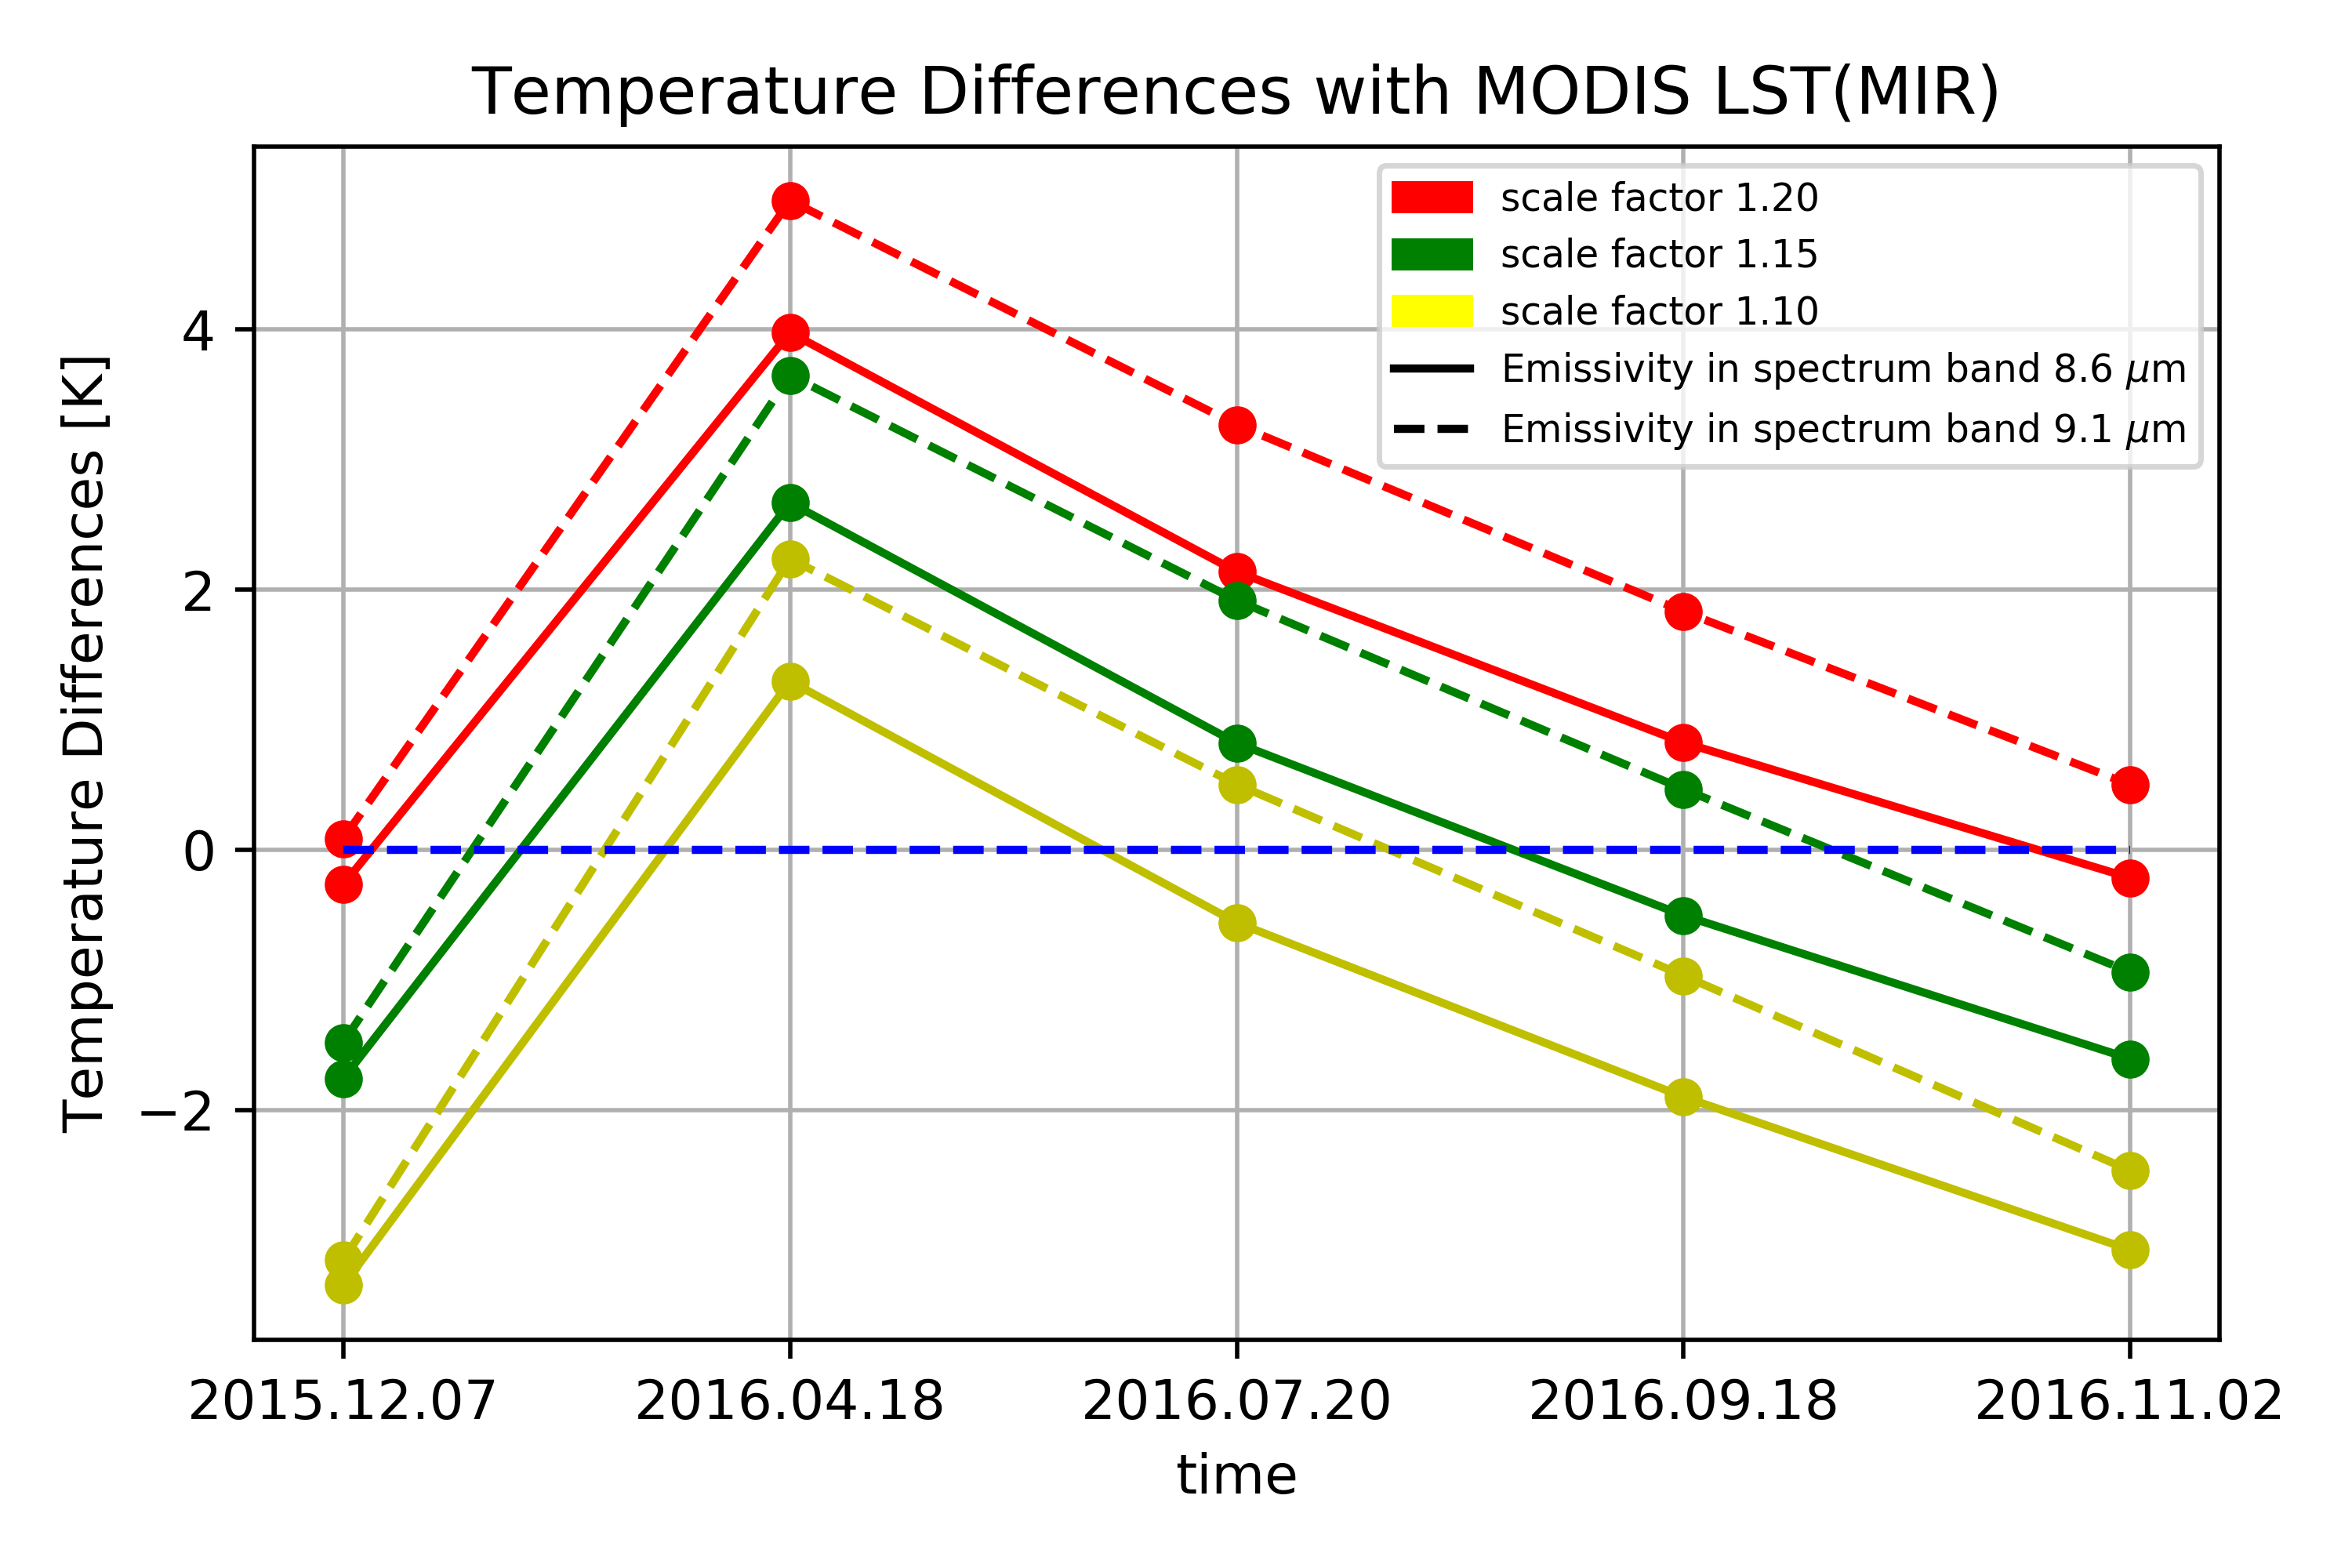
\includegraphics[width = 0.8\textwidth]{diff_emi_mir1.png}
\caption{Temperature differences (Lybia-1) between the surface temperature maps in MIR band and MODIS LST.}
\label{fig:diff_emi_mir1}
\end{figure}

\noindent Concentrate on one certain scale factor, as shown in Figure \ref{fig:diff_emi_Lybia2}, we can see that using the emissivity map with spectral band 9.1 $\mu$m, the temperature differences between the surface temperature maps from MITIP and MODIS LST is much higher than those using the emissivity map with spectral band 8.6 $\mu$m. Besides, in order to keep consistent with the comparison with the MODIS SST, the emissivity map with spectral band 8.6 $\mu$m will be reminded in use.\\

\begin{figure}[!htbp]
\centering
\subfigure[MIR band]{
\label{fig:diff_emi_mir2}
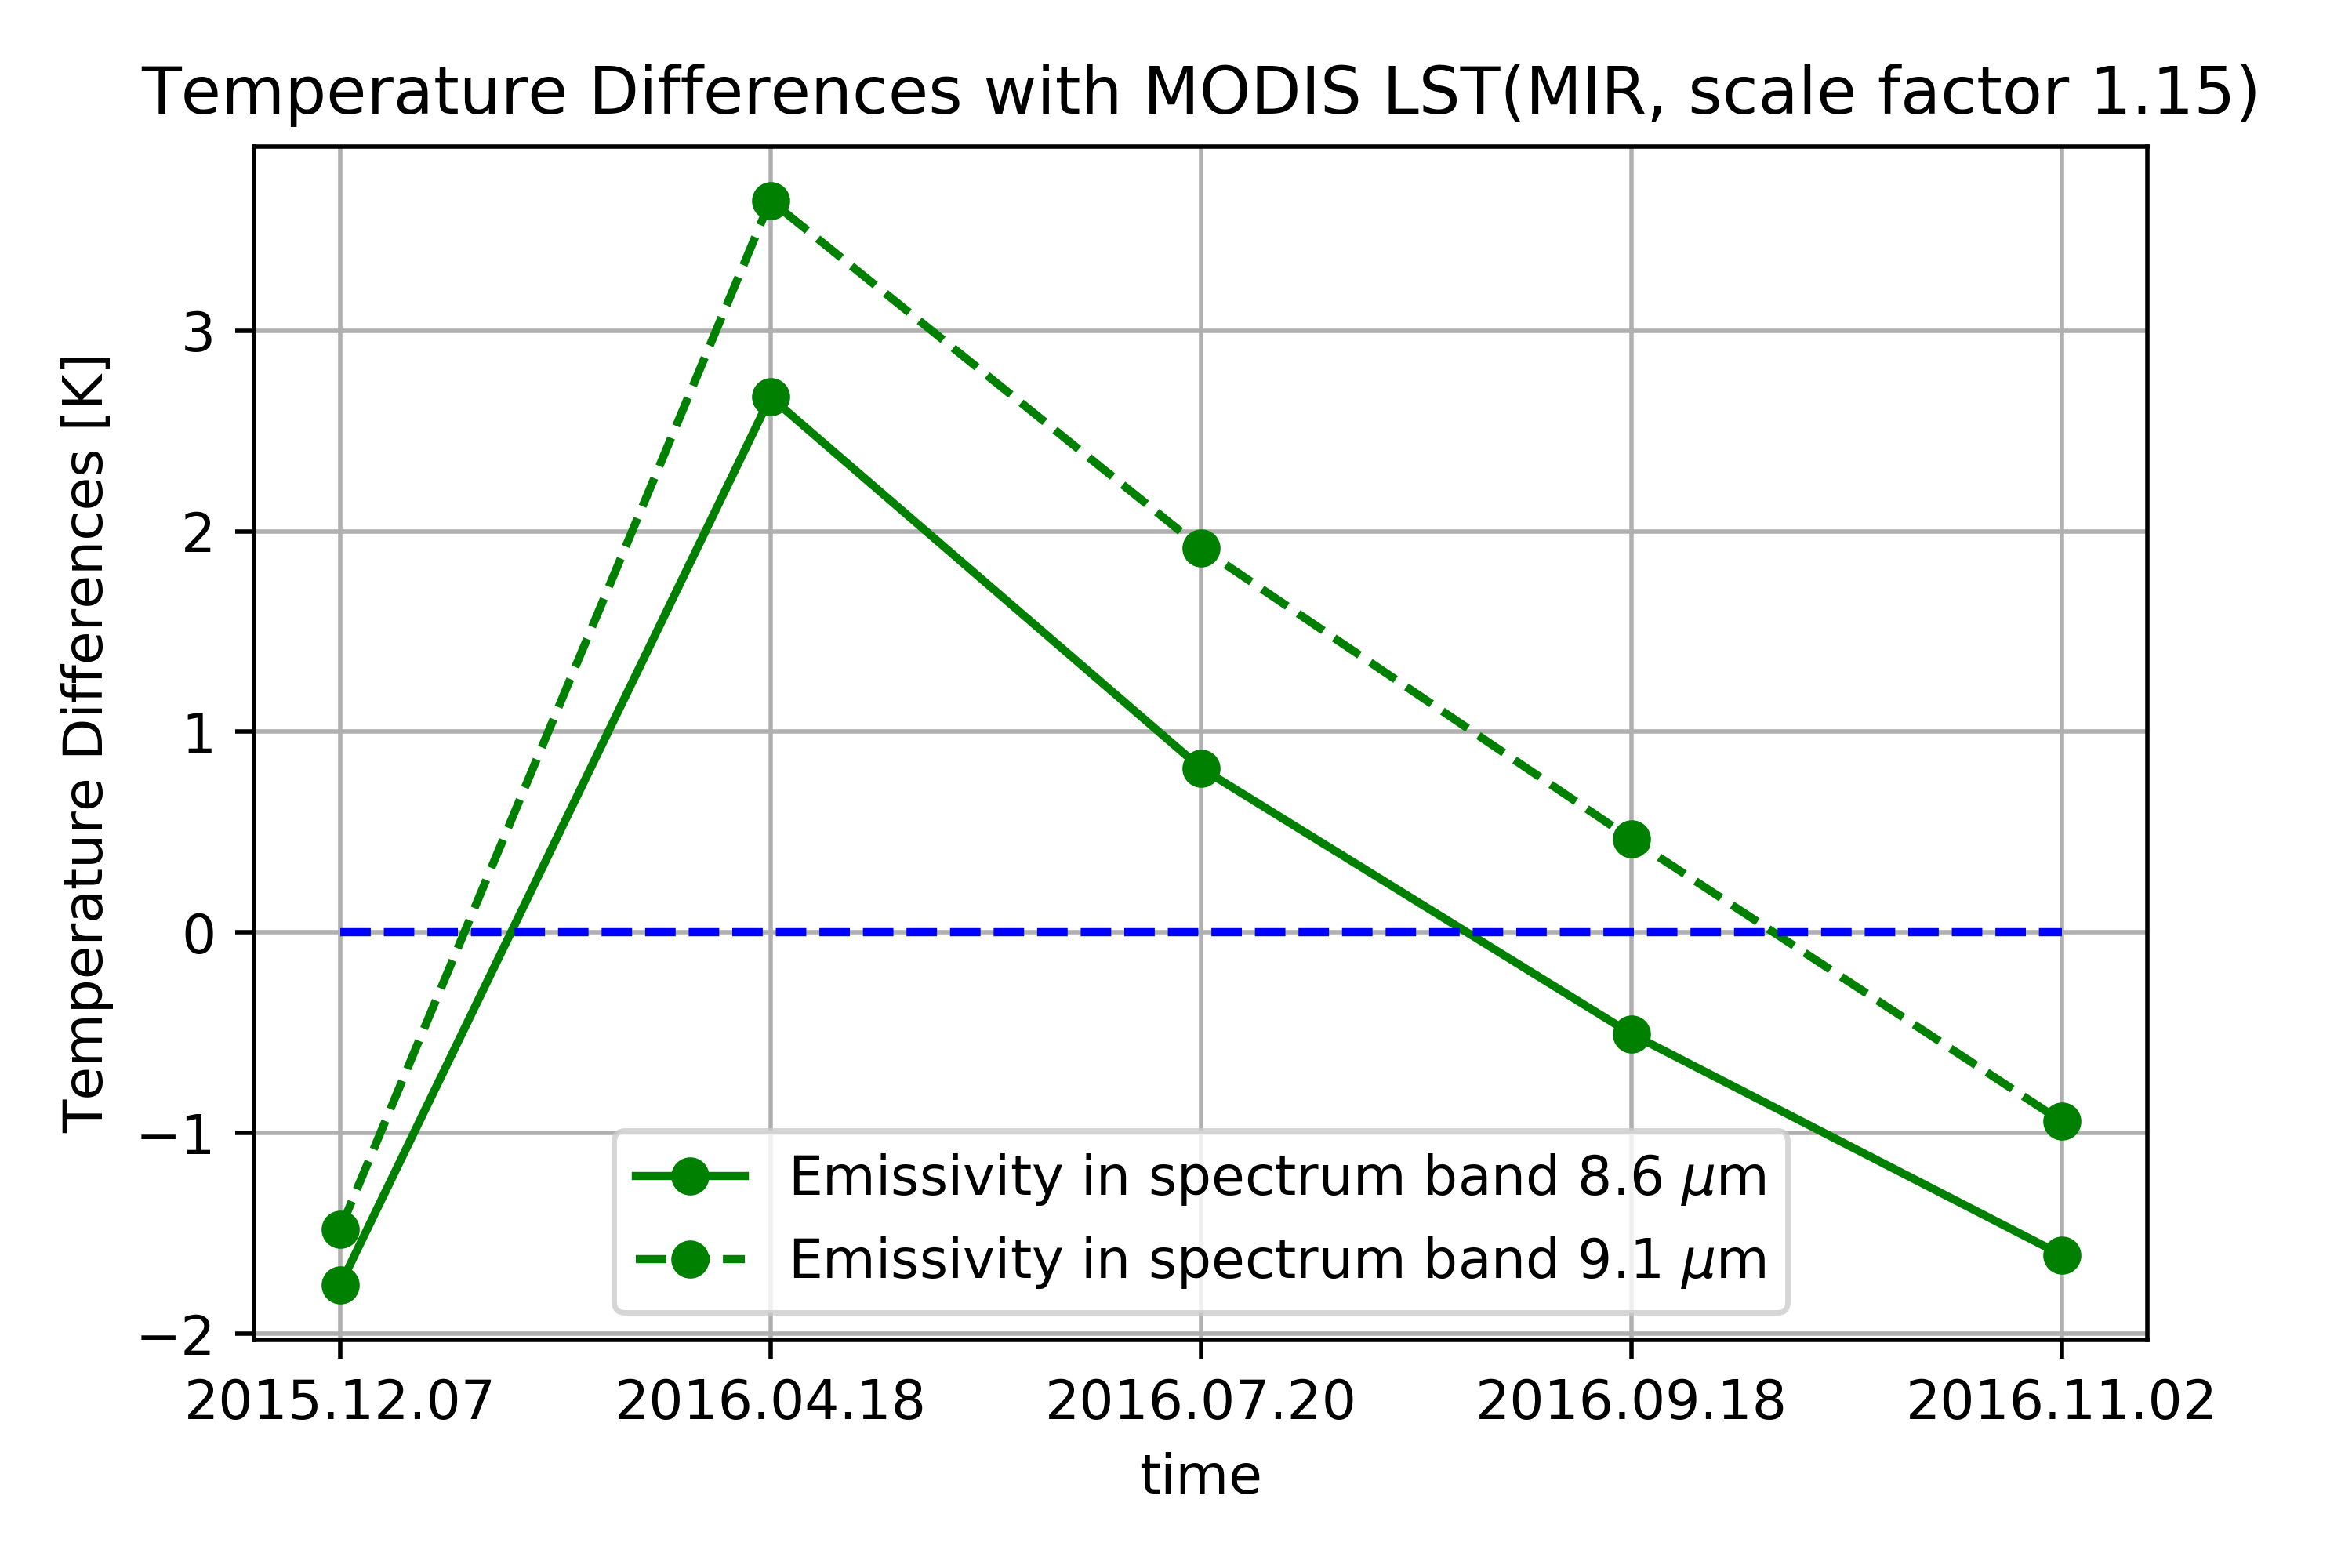
\includegraphics[width = 0.8\linewidth]{diff_emi_mir2.png}}
\hspace{0.5in}
\subfigure[TIR band]{
\label{fig:diff_emi_tir2}
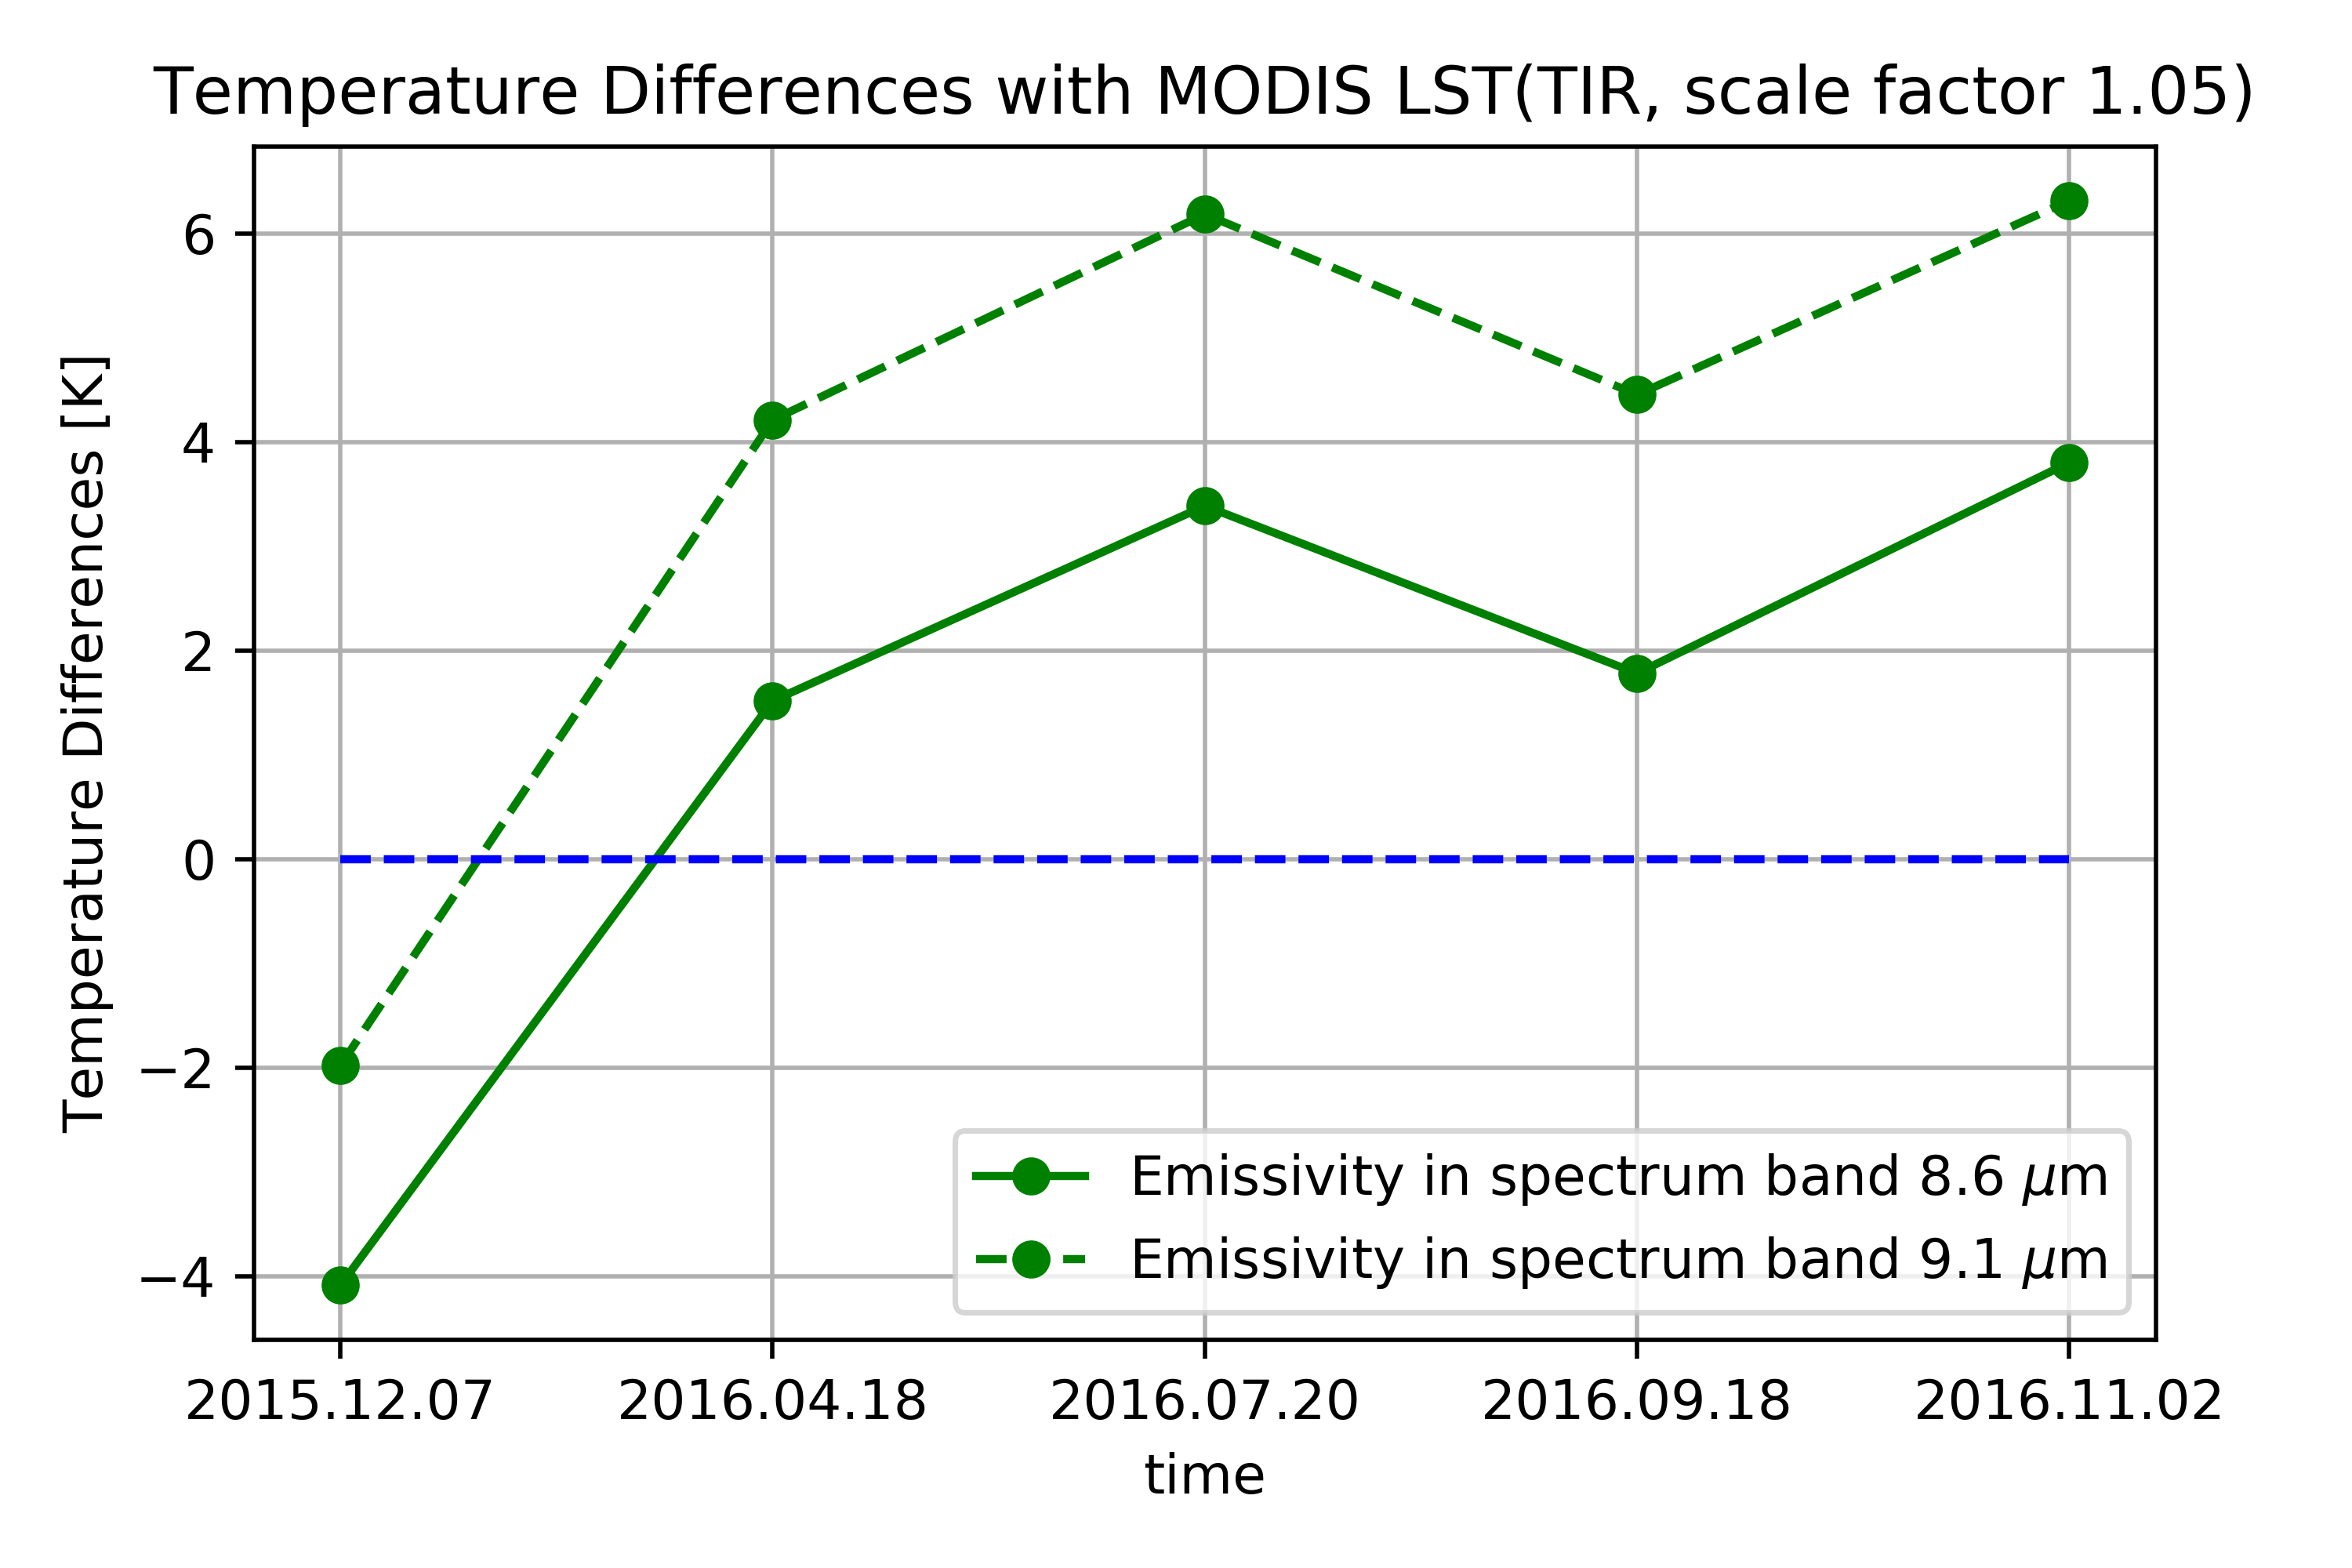
\includegraphics[width = 0.8\linewidth]{diff_emi_tir2.png}}
\caption{Temperature differences (Lybia-1) between the surface temperature maps from MITIP with certain scale factor and MODIS LST.}
\label{fig:diff_emi_Lybia2}
\end{figure}

\noindent After choosing an appropriate emissivity map, similar comparisons between TET-1 surface temperature maps and MODIS LST can be carried out. As what has been done in previous section, several sub-areas are selected distributed over the Libya-1 scenes and the mean temperature difference over all the sub-areas are used to do the comparisons as well.\\

\begin{figure}[!htbp]
\centering
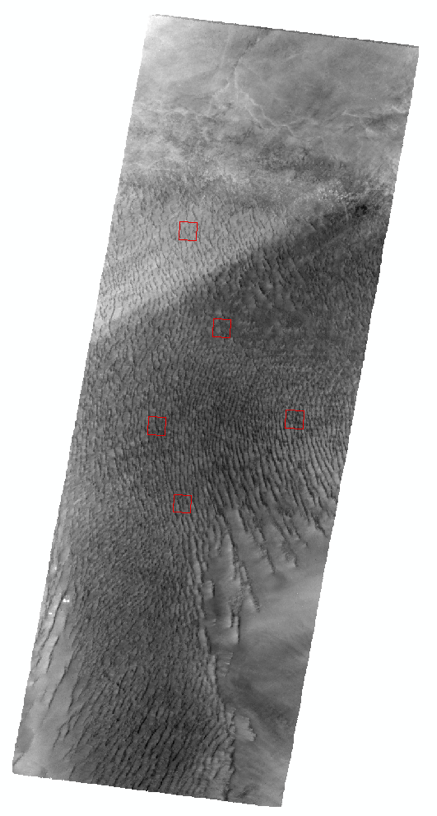
\includegraphics[width = 0.5\textwidth]{Libya-1.png}
\caption{The example figure of Libya-1. The red rectangles represent the selected sub-areas.}
\label{fig:Libya1_sub_areas}
\end{figure}

\begin{figure}[!htbp]
\centering
\subfigure[MIR band]{
\label{fig:Libya-1_sc_mir}
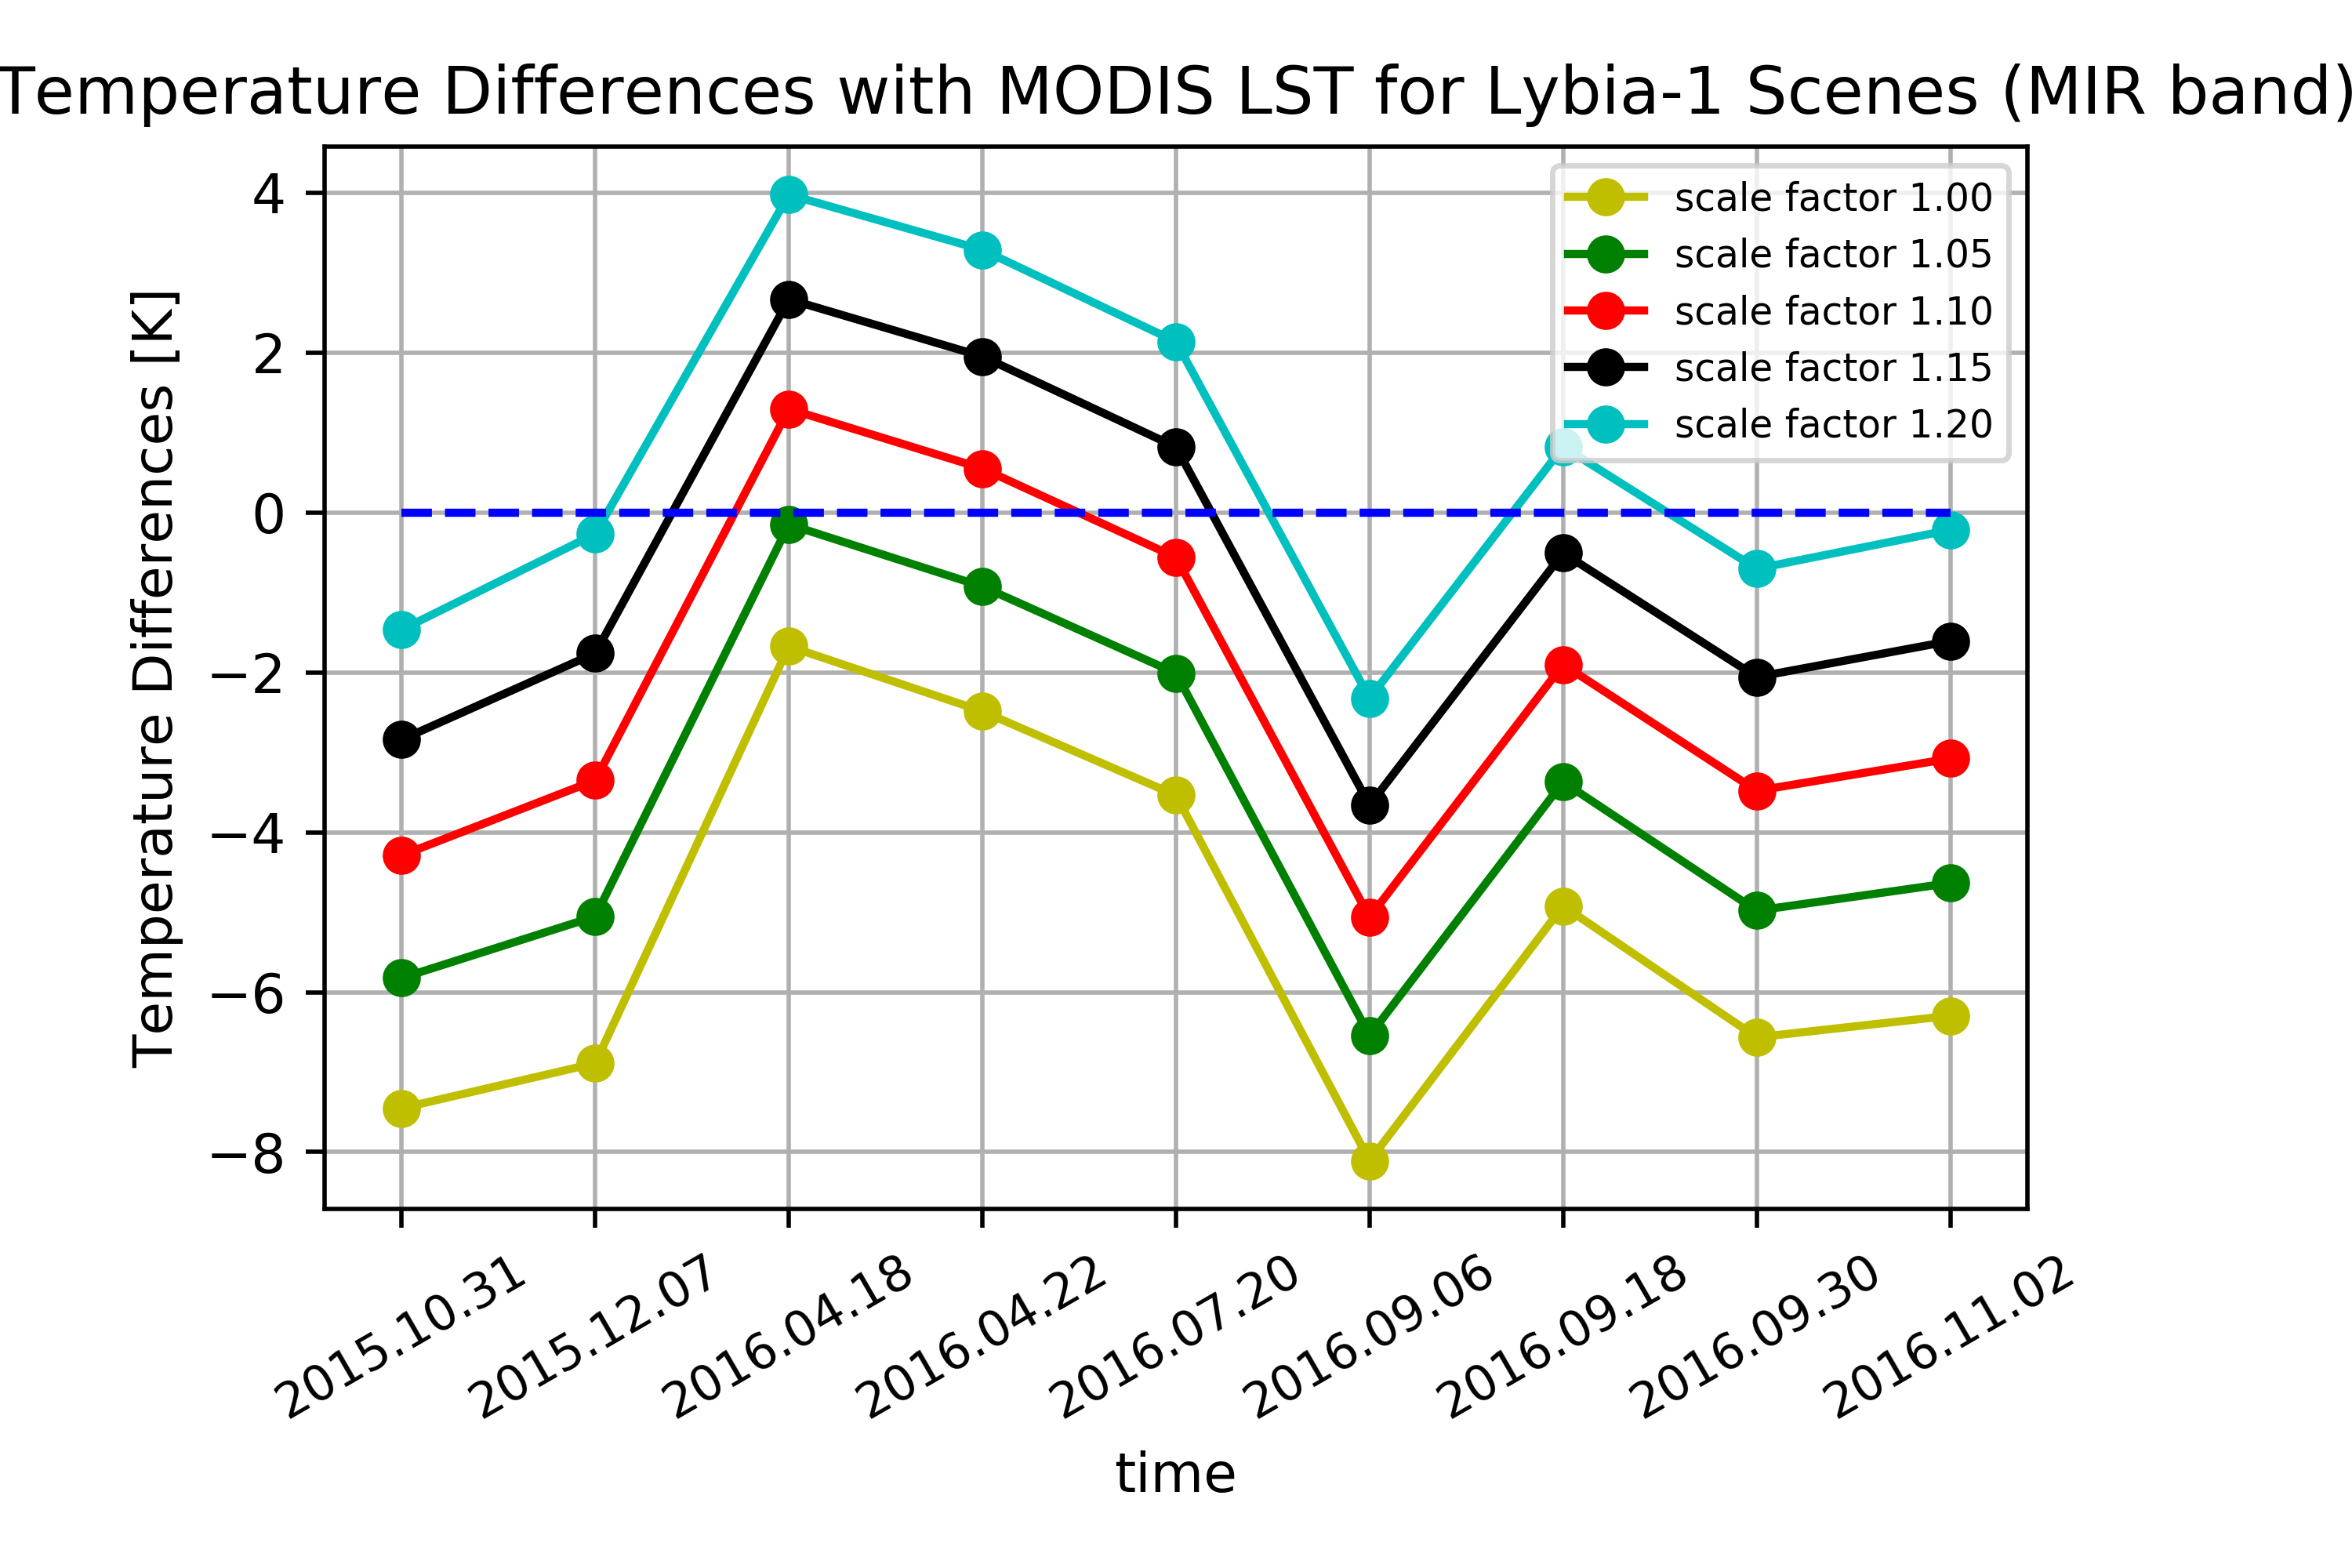
\includegraphics[width = 0.8\linewidth]{Lybia-1_scf_mir.png}}
\hspace{0.5in}
\subfigure[TIR band]{
\label{fig:Libya-1_sc_tir}
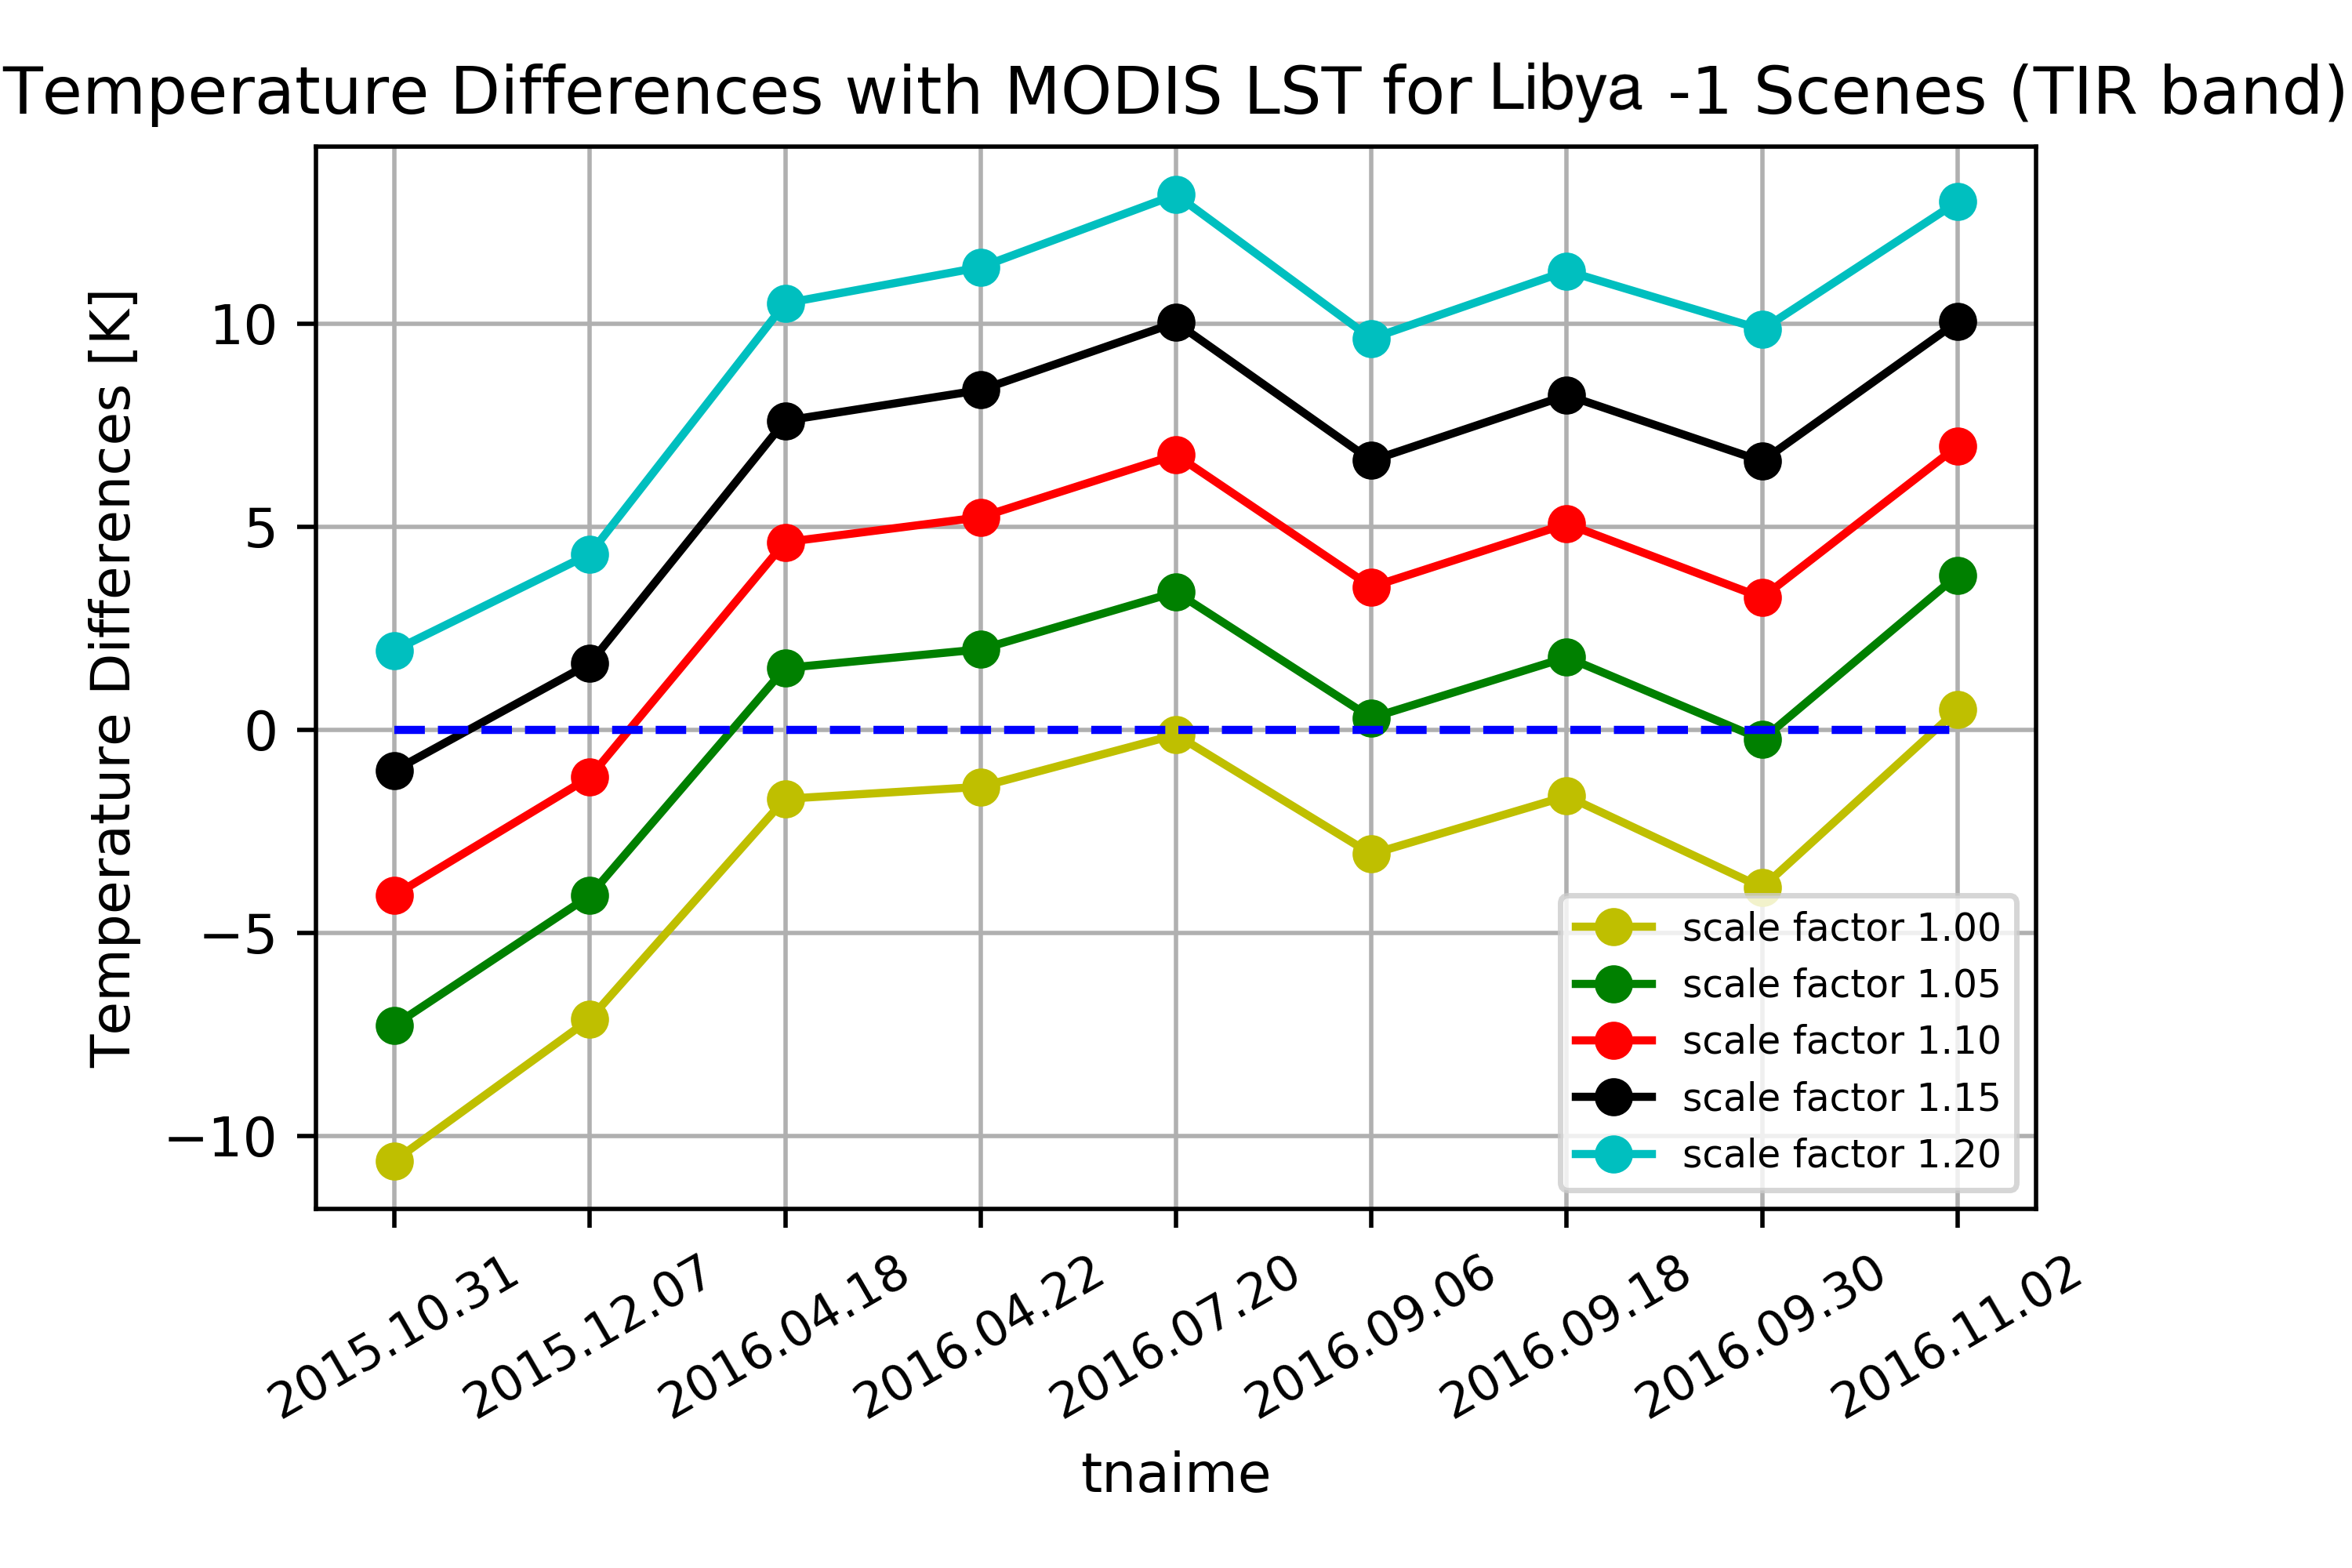
\includegraphics[width = 0.8\linewidth]{Lybia-1_scf_test_tir.png}}
\caption{Tempereature differences between TET-1 surface temperature maps and MODIS LST (Libya-1).}
\label{fig:Libya-1_sc_mir_tir}
\end{figure}

\noindent As Figure \ref{fig:Libya-1_sc_mir_tir} shows, the temperature differences between MODIS LST and TET-1 surface temperature maps with different scale factors act randomly as well. For the TIR band imageries, again, the scale factor 1.05 achieves the best performances, which can also be seen in Figure \ref{fig:Libya-1_bsc_tir}. For the MIR band imageries, it is clear from the Figure \ref{fig:Libya-1_sc_mir} and Figure \ref{fig:Libya-1_bsc_mir}, much more MIR band imageries require a higher scale factor compared with the situation of doing comparison with the MODIS SST. This is also why the scale factor 1.15 is selected as the optimal scale factor for the MIR band imageries. On one hand, it can achieve a good results for these scenes require a higher scale factor. On the other hand, it will not over calibrate these scenes require a lower scale factor. All in all, the scale factor 1.15 for the MIR band imageries perform best over all scenes of different times.\\

\begin{figure}[!htbp]
\centering
\subfigure[MIR band]{
\label{fig:Libya-1_bsc_mir}
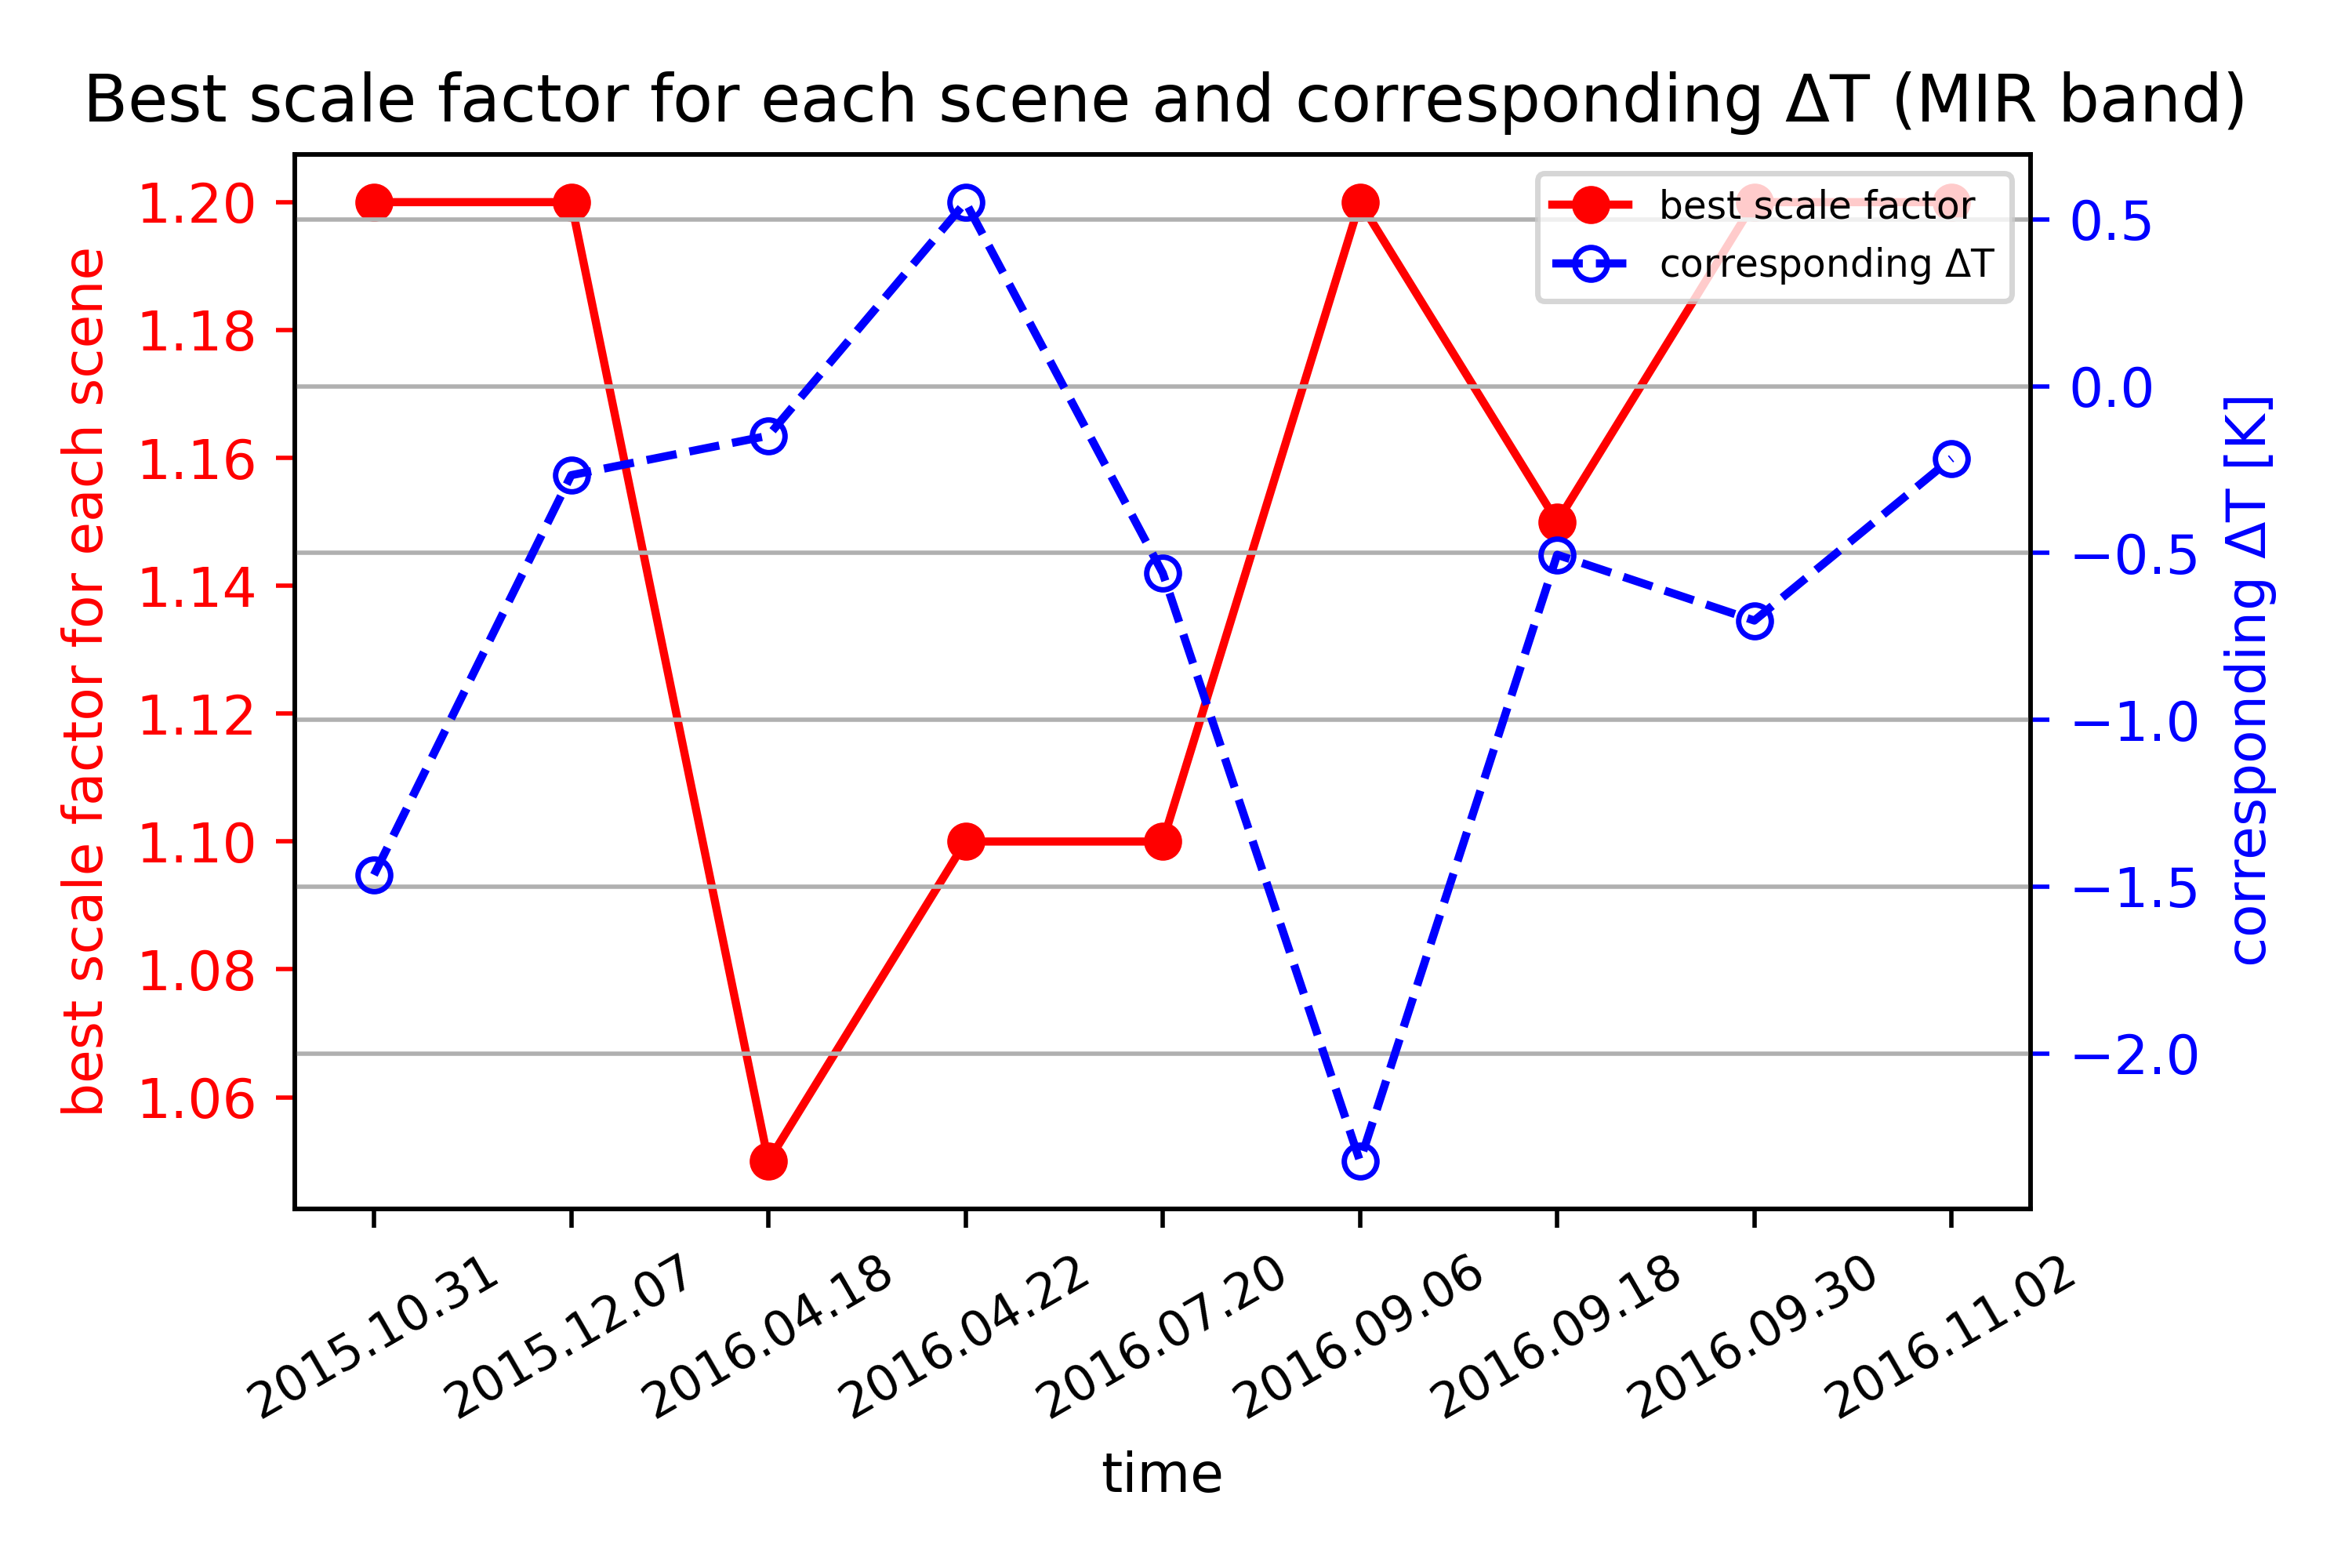
\includegraphics[width = 0.8\linewidth]{Lybia-1_bsc&tem_mir.png}}
\hspace{0.5in}
\subfigure[TIR band]{
\label{fig:Libya-1_bsc_tir}
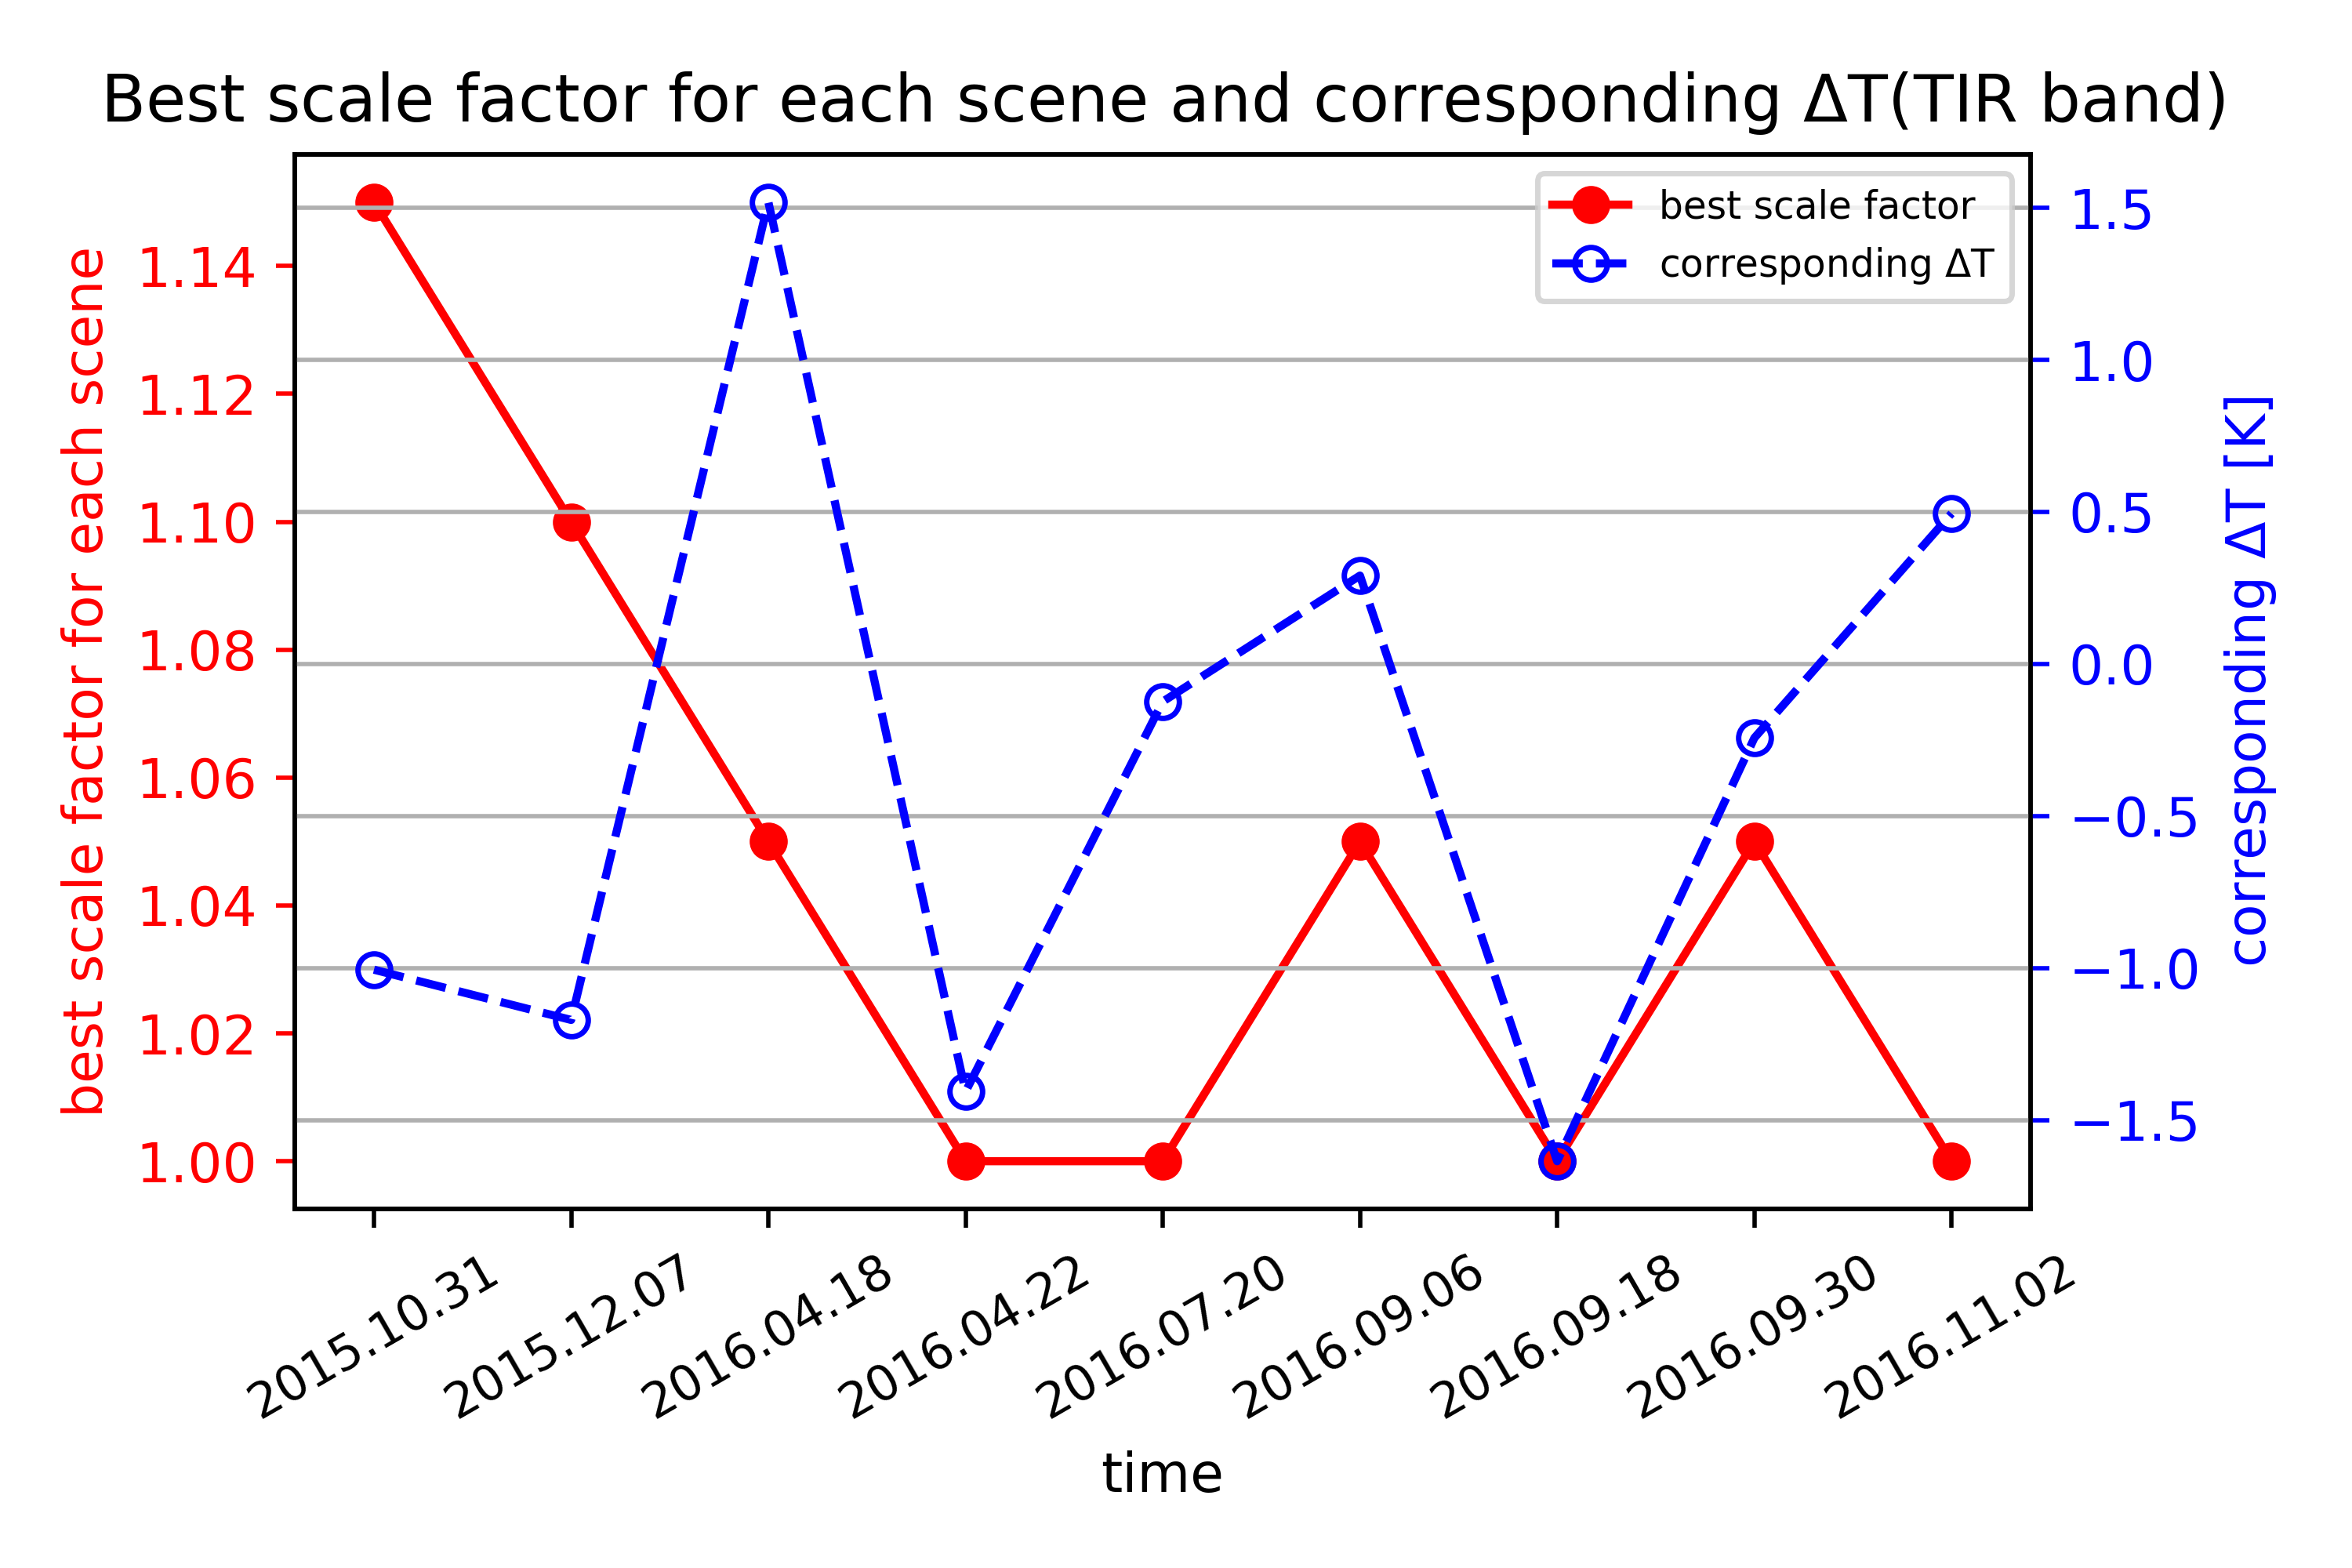
\includegraphics[width = 0.8\linewidth]{Lybia-1_bsc&tem_tir.png}}
\caption{The best scale factors for each Lybia-1 scenes and its corresponding temperature differences. The red solid line is the best scale factor for each Libya-1 scene. The blue dashed line is the minimal temperature differences resulted from that scale factor.}
\label{fig:Libya-1_bsc_mir_tir}
\end{figure}

\begin{figure}[!htbp]
\centering
\subfigure[MIR band]{
\label{fig:Lybia-1_bsc&temCom_mir}
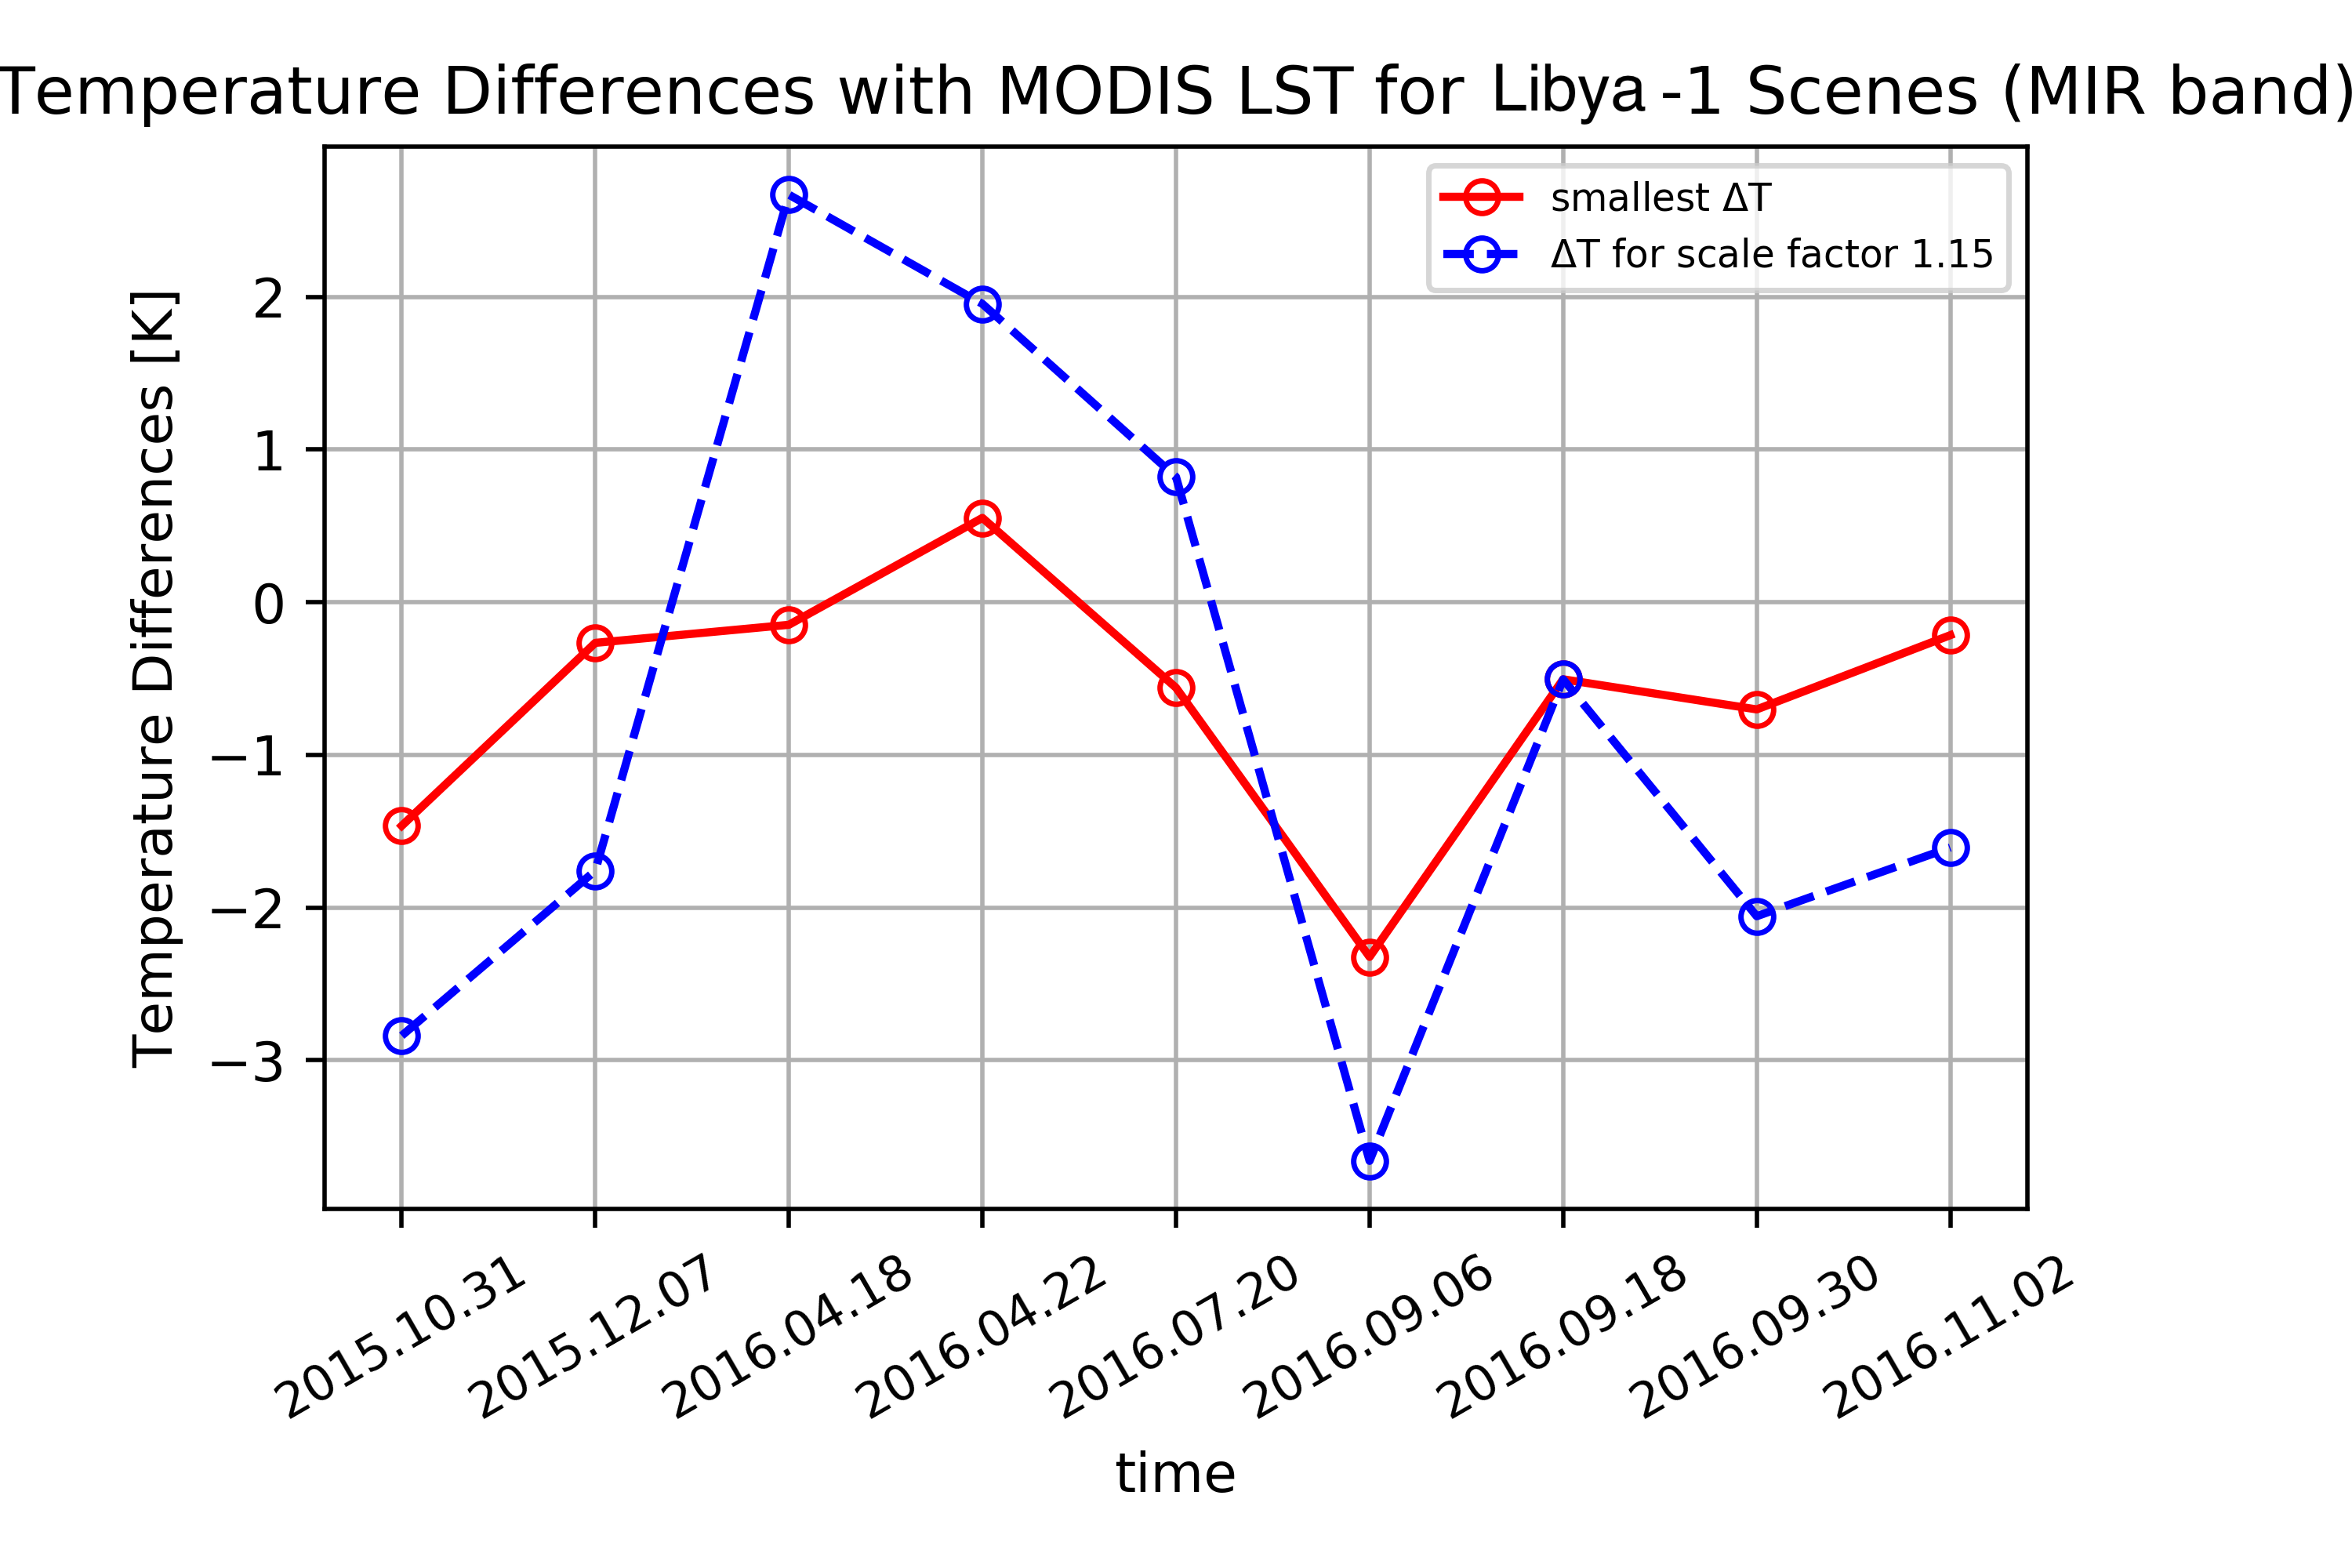
\includegraphics[width = 0.8\linewidth]{Lybia-1_bsc&temCom_mir.png}}
\hspace{0.5in}
\subfigure[TIR band]{
\label{fig:Lybia-1_bsc&temCom_tir}
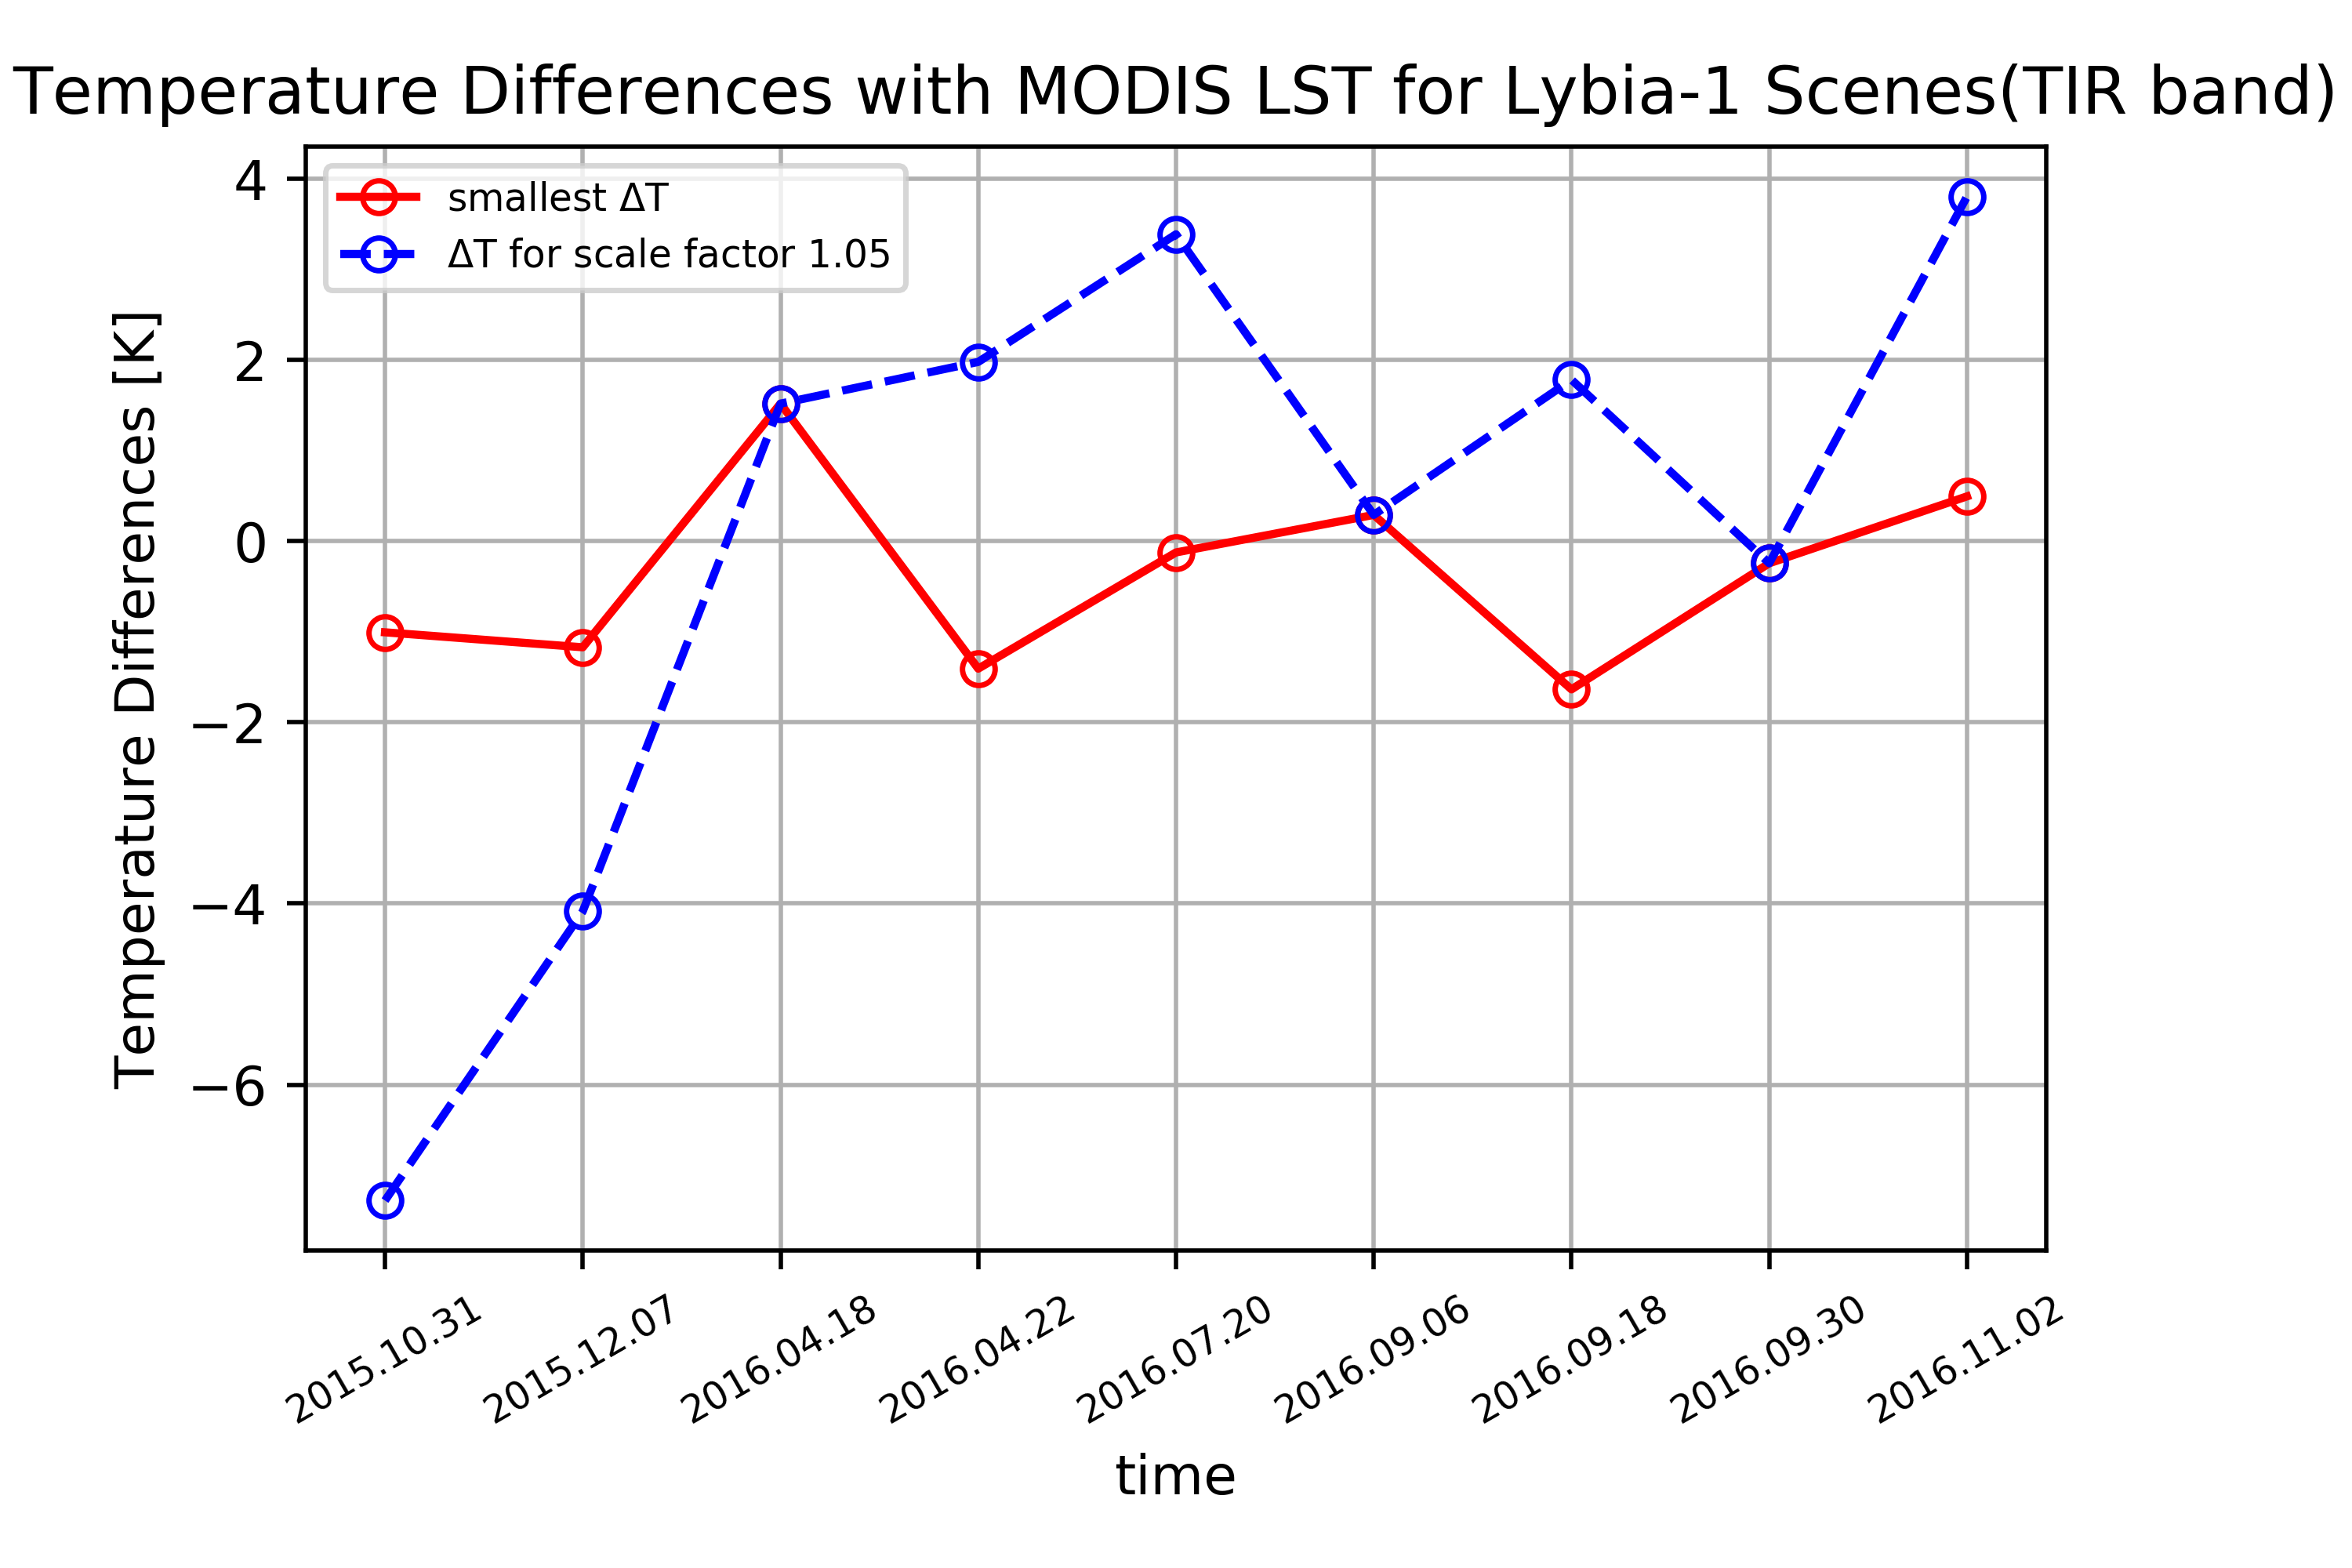
\includegraphics[width = 0.8\linewidth]{Lybia-1_bsc&temCom_tir.png}}
\caption{The minimal temperature differences and the temperature differences resulted from scale factor 1.15 and scale factor 1.05. The red solid line is the minimal temperature differences for each Etna scene. The blue dashed line is the temperature differences resulted from the selected scale factors for MIR and TIR band imageries, scale factor 1.15 (upper) and scale factor 1.05 (lower), respectively.}
\label{fig:Lybia-1_bsc&temCom}
\end{figure}

\noindent As Figure \ref{fig:Lybia-1_bsc&temCom} shows, for the TET-1 MIR and TIR band imageries of the site Libya-1, the scale factor 1.15 and 1.05 are not the optimal scale factors for every scene. But the temperature differences they made are very close to the minimal temperature differences. What's more, the choices enable us to ignore the difference between water-dominated or land-dominated scenes because the optimal scale factors for the Libya-1 scenes are the same as the optimal scale factors for the Etna scenes. Of course, latter, the transferability of the scale factors selected from the Libya-1 scenes will be tested.\\

%-----------------------------------
%	SUBSECTION 5
%-----------------------------------

\subsection{transferability test (LST)}
After the selection of the optimal scale factors, as what has been done after the comparisons with the MODIS SST, the transferability of  the chosen scale factors will be tested using several scenes of other sites. Here, scenes of Libya-2 are used as test scenes. Figure \ref{fig:Libya2_sub_areas} is an example scene of Libya-2.\\

\begin{figure}[!htbp]
\centering
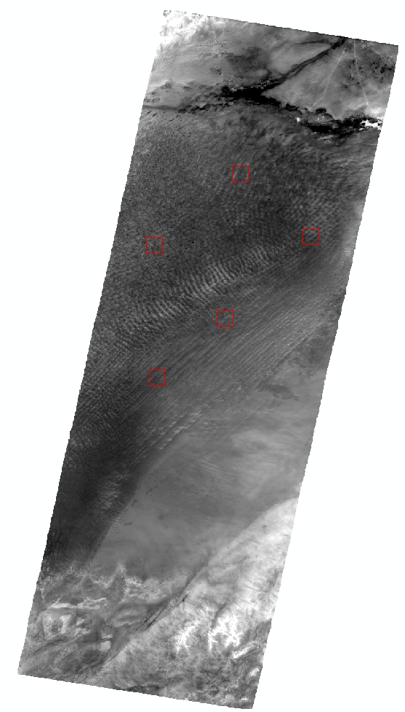
\includegraphics[width = 0.5\textwidth]{Libya-2.png}
\caption{The example figure of Libya-2. The red rectangles represent the selected sub-areas.}
\label{fig:Libya2_sub_areas}
\end{figure}

\noindent Besides the chosen scale factor 1.15 for MIR band imagery and 1.05 for TIR band imagery, the performance of the scale factor 1.10 and 1.20 are also presented for the TET-1 MIR band imagery as comparison and for TIR band imagery, the performances of scale factor 1.00 and 1.10 are displayed as well for the same purpose. The results arde presented in Figure \ref{fig:LST_test}. The situation is similar with the situation of Section 4.1.3. Scale factor 1.15 for MIR band imagery and 1.05 for TIR band imagery are not always optimal scale factors for every scenes, however, they demonstrate better performance than other scale factors over time.\\

\begin{figure}[!htbp]
\centering
\subfigure[MIR band]{
\label{fig:LST_test_mir}
\includegraphics[width = 0.8\linewidth]{lls_test&cmp_mir.png}}
\hspace{0.5in}
\subfigure[TIR band]{
\label{fig:LST_test_tir}
\includegraphics[width = 0.8\linewidth]{lls_test&cmp_tir.png}}
\caption{Transferability test: temperature differences between TET-1 surface temperature maps and MODIS LST.}
\label{fig:LST_test}
\end{figure}

%----------------------------------------------------------------------------------------
%	SECTION 2
%----------------------------------------------------------------------------------------

\section{Conclusion of the comparisons and calibrations}
In this chapter, the MITIP method are tested using the Etna scenes and improved by adding two key words \emph{sc1} and \emph{sc2} to calibrate the TOA radiances of the TET-1 MIR and TIR band imagery respectively. In order to find the best scale factors for the TET-1 MIR and TIR band imageries separately, the surface temperature maps in MIR band TIR band are compared with the MODIS SST firstly and then LST respectively. After all of the comparisons and tests, the optimal scale factors for TET-1 MIR and TIR band imageries are chosen as 1.15 and 1.05 respectively. Both of the scale factors performs well in both space and time domain. Later, the MITIP method will be applied to several high-temperature events scenes with the determined scale factors.\\
%-----------------------------------
%	SUBSECTION 1
%-----------------------------------

% \subsection{Data preparasion}

%-----------------------------------
%	SUBSECTION 2
%-----------------------------------

% \subsection{Outcomes of the mitip and results comparision with MODIS LST}

%-----------------------------------
%	SUBSECTION 3
%-----------------------------------

% \subsection{Calibrations}

%-----------------------------------
%	SUBSECTION 4
%-----------------------------------

% \subsection{Test of the results of calibrations}


\chapter{Analysis of high-temperature events}

\label{Chapter5}

In this chapter, the products of HTE monitoring from MITIP will presented firstly using scenes worldwide which contains volcanoes, large scale lava flow and wild fires. In section 5.2, the HTE monitoring results of MITIP will be compared with the results of the Zhukov's algorithm, which is used to process the TET-1 imagery originally.\\
%----------------------------------------------------------------------------------------
%	SECTION 1
%----------------------------------------------------------------------------------------

\section{High-temperature events}
In this section, the HTE monitoring results are presented. For the processing of all scenes, the maps of MODIS water vapor, ASTER DEM and 8.6 $\mu$m emissivity maps were provided and resampled to the TET-1 imagery's size and pixel size. The input TET-1 MIR and TIR TOA radiance imageries are scaled with scale factor 1.15 and 1.05 respectively.\\

%-----------------------------------
%	SUBSECTION 1
%-----------------------------------

\subsection{Volcanoes}
First of all, the HTE monitoring products of Etna and Stromboli in the date 2016.06.22 are presented. Both of them only occupy a little spaces in images because of their small sizes.\\

\begin{figure}[!htbp]
\centering
\subfigure[MIR band]{
\label{fig:Etna_mir_tem}
\includegraphics[width = 0.8\linewidth]{temp_map_etna_mir.png}}
\hspace{0.1in}
\subfigure[TIR band]{
\label{fig:Etna_tir_tem}
\includegraphics[width = 0.8\linewidth]{temp_map_etna_tir.png}}
\caption{Surface temperature maps of Etna 2014.06.22.}
\label{fig:Etna_sur_tem}
\end{figure}

\noindent As Figure \ref{fig:Etna_sur_tem} shows, the surface temperatures of the lava are around 310 K to 340K in MIR band and 290K to 310K in TIR band. The effective target temperature in sub-pixel resolution and effective target pixel fraction as well as the FRP are shown in Figure \ref{fig:Etna_HTE} and Figure \ref{fig:Etna_frp}. We can see that not all hot pixels in the surface temperature maps are solved for the effective target temperature and target pixel fraction due to numerical reasons. The hottest areas of the Etna are around 850 K. It can be notice that the higher the effective target temperature in one pixel is, the lower the effective target pixel fraction of it is. Because the pixel temperature and background temperature are pre-determined.\\

\begin{figure}[!htbp]
\centering
\subfigure[Effective target temperature]{
\label{fig:Etna_eff_tem}
\includegraphics[width = 0.8\linewidth]{Effective_target_tem_etna.png}}
\hspace{0.1in}
\subfigure[Effective target pixel fraction]{
\label{fig:Etna_eff_fra}
\includegraphics[width = 0.8\linewidth]{Effective_target_pixel_frac_etna.png}}
\caption{HTE monitoring products of Etna 2014.06.22.}
\label{fig:Etna_HTE}
\end{figure}

\begin{figure}[!htbp]
\centering
\includegraphics[width=0.8\linewidth]{frp_etna.png}
\caption{FRP of Etna 2014.06.22.}
\label{fig:Etna_frp}
\end{figure}

\noindent Stromboli island is one of the Aeolian island of Italy. The Stromboli volcano is one of the most active volcanoes on Earth. It has been nearly continuous erupting for about 2000 years. Since there is a small town in Stromboli island, the prediction and monitoring of the eruption of the Stromboli volcano is of great importance. The figure \ref{fig:Strom_sur_tem} shows the surface temperature maps of Stromboli in MIR and TIR band respectively of the date 2014.06.22. It can be noticed that in evening, the temperature of the sea surface is higher than the temperature of the land surface.\\

\begin{figure}
\centering
\subfigure[MIR band]{
\label{fig:Strom_mir_tem}
\includegraphics[width = 0.8\linewidth]{strom_tem_mir.png}}
\hspace{0.1in}
\subfigure[TIR band]{
\label{fig:Strom_tir_tem}
\includegraphics[width = 0.8\linewidth]{strom_tem_tir.png}}
\caption{Surface temperature maps of Stromboli 2014.06.22.}
\label{fig:Strom_sur_tem}
\end{figure}

\noindent The effective target temperature and effective target pixel fraction of Stromboli in date 2014.06.22 are shown in Figure \ref{fig:Strom_HTE} and the fire radiative power in Figure \ref{fig:Strom_frp}. We can see that the hottest areas of the Stromboli is above 1400 K which only occupy a small fraction of the pixels as well.\\

\begin{figure}[!htbp]
\centering
\subfigure[Effective target temperature]{
\label{fig:Strom_eff_tem}
\includegraphics[width = 0.8\linewidth]{strom_eff_tem_strom.png}}
\hspace{0.1in}
\subfigure[Effective target pixel fraction]{
\label{fig:Strom_eff_fra}
\includegraphics[width = 0.8\linewidth]{strom_eff_pixel_frac_strom.png}}
\caption{HTE monitoring products of Stromboli 2014.06.22.}
\label{fig:Strom_HTE}
\end{figure}

\begin{figure}[!htbp]
\centering
\includegraphics[width=0.8\linewidth]{frp_strom.png}
\caption{FRP of Stromboli 2014.06.22.}
\label{fig:Strom_frp}
\end{figure}

\noindent Etna and Stromboli are both small volcanoes which occupy only a few pixels in the imageries. In contrast, the eruption of Bardarbunga is much more intensive and its lava occupies a much larger area. Bardarbunga is a subglacial stratovolcano located in Iceland. The last eruption of Bardarbunga is from August 2014 to February 2015. Figure \ref{fig:Bar_sur_tem} presents the surface temperature map of Bardarbunga in date 2014.09.14.\\

\begin{figure}
\centering
\subfigure[MIR band]{
\label{fig:Bar_mir_tem}
\includegraphics[width = 0.8\linewidth]{Bar_tem_mir.png}}
\hspace{0.1in}
\subfigure[TIR band]{
\label{fig:Bar_tir_tem}
\includegraphics[width = 0.8\linewidth]{Bar_tem_tir.png}}
\caption{Surface temperature maps of Bardarbunga 2014.09.14.}
\label{fig:Bar_sur_tem}
\end{figure}

\noindent It is clear that the erupted lava occupied a large area and the temperature of it is between 400 K and 500 K in MIR band and 350 K to 450 K in TIR band. Figure \ref{fig:Bar_HTE} and Figure \ref{fig:Bar_frp} give the effective target temperature and effective target pixel fraction as well as FRP maps.\\

\begin{figure}[!htbp]
\centering
\subfigure[Effective target temperature]{
\label{fig:Bar_eff_tem}
\includegraphics[width = 0.8\linewidth]{Bar_eff_tem.png}}
\hspace{0.1in}
\subfigure[Effective target pixel fraction]{
\label{fig:Bar_eff_fra}
\includegraphics[width = 0.8\linewidth]{Bar_eff_pixel_frac.png}}
\caption{HTE monitoring products of Bardarbunga 2014.09.14.}
\label{fig:Bar_HTE}
\end{figure}

\begin{figure}[!htbp]
\centering
\includegraphics[width=0.8\linewidth]{Bar_frp.png}
\caption{FRP of Bardarbunga 2014.09.14.}
\label{fig:Bar_frp}
\end{figure}
%-----------------------------------
%	SUBSECTION 2
%-----------------------------------

\subsection{Fire events}
Besides volcanoes, wild fires are another kind of high-temperature events need to be paid attention to. Here, the HTE monitoring results of Portugal wild fires is presented. Figure \ref{fig:Por_sur_tem} shows the surface temperature maps in MIR and TIR band. The fire edges can be seen clearly in the surface temperature maps.\\

\begin{figure}
\centering
\subfigure[MIR band]{
\label{fig:Por_mir_tem}
\includegraphics[width = 0.8\linewidth]{Por_tem_mir.png}}
\hspace{0.1in}
\subfigure[TIR band]{
\label{fig:Por_tir_tem}
\includegraphics[width = 0.8\linewidth]{Por_tem_tir.png}}
\caption{Surface temperature maps of Portugal wild fires in 2016.08.11.}
\label{fig:Por_sur_tem}
\end{figure}

\noindent Figure \ref{fig:Por_HTE} and Figure \ref{fig:Por_frp} are the effective target temperature and effective target pixel fraction as well as fire radiative power maps. We can see the large scale and the scorching temperatures of the wild fires.

\begin{figure}[!htbp]
\centering
\subfigure[Effective target temperature]{
\label{fig:Por_eff_tem}
\includegraphics[width = 0.8\linewidth]{Por_eff_tem.png}}
\hspace{0.1in}
\subfigure[Effective target pixel fraction]{
\label{fig:Por_eff_fra}
\includegraphics[width = 0.8\linewidth]{Por_eff_pixel_frac.png}}
\caption{HTE monitoring products of Portugal wild fires in 2016.08.11.}
\label{fig:Por_HTE}
\end{figure}

\begin{figure}[!htbp]
\centering
\includegraphics[width=0.8\linewidth]{Por_frp.png}
\caption{FRP of Portugal wild fires in 2016.08.11.}
\label{fig:Por_frp}
\end{figure}

%----------------------------------------------------------------------------------------
%	SECTION 2
%----------------------------------------------------------------------------------------

\section{Comparison with the results of the Zhukov's algorithm}
In this section, the HTE monitoring products of MITIP are compared with the results of Zhukov's algorithm, which used to process the TET-1 imagery originally.\\

%-----------------------------------
%	SUBSECTION 1
%-----------------------------------

\subsection{Brief description of Zhukov's algorithm}
Unlike other hot spot detection algorithms, the Zhukov's algorithm carries out a bundle of tests to filter out clouds, warm surfaces and sun glints etc first and then performs fire pixel detection. It uses the dual channel method stated in Chapter 2 to determine effective fire temperature in sub-pixel resolution as well. However, the Zhukov's algorithm detects and quantifies the hot area by means of per cluster instead of per pixel as MITIP method dose. After the detection of hot pixels, the Zhukov's algorithm aggregates hot pixels which are adjacent to each other to form a hot cluster and the temperature of this cluster and its area etc are estimated.\\

\begin{figure}[!htbp]
\centering
\includegraphics[width=0.8\linewidth]{Zhukov_algorithm.jpg}
\caption{Flow chart of the Zhukov's algorithm.}
\label{fig:Zhu_alg}
\end{figure}

\noindent The brief procedure of Zhukov's algorithm is shown in Figure \ref{fig:Zhu_alg}.\\

%-----------------------------------
%	SUBSECTION 2
%-----------------------------------

\subsection{From pixel-based to cluster-based analysis}
In contrast to Zhukov's algorithm, the MITIP method performs a pixel-based analysis. Consequently, in order to compare the results of the MITIP method and Zhukov's algorithm, here a procedure is developed to shift the MITIP's original pixel-based results to a cluster-based results because it is much more difficult to derive each pixel's temperature from the characteristics of the whole cluster. \\

\noindent The procedure is described as follows. The input is the effective target pixel fraction map and effective target temperature map which is converted to a vector file afterwards. The connected pixels will then form a polygon feature with which a cluster will come into being. Then every polygon feature in the vector file is extracted and converted to a raster file acts as a mask file. The mask file is used to extract AOI in the effective target temperature map and zonal statistics is carried out over the AOI. The final output is the cluster's temperature and size. The cluster's temperature is the weighted average of the effective target temperatures of pixels within this cluster and the weights are the corresponding effect target pixel fractions. The size of the cluster is denoted by the number of pixels. The Figure \ref{fig:P2C} shows the flow chart of the described procedure.\\

\begin{figure}[!htbp]
\centering
\includegraphics[width=0.4\linewidth]{Procedure.png}
\caption{Flow chart of the pixel-based result to the cluster-based result.}
\label{fig:P2C}
\end{figure}

%-----------------------------------
%	SUBSECTION 3
%-----------------------------------

\subsection{Comparison}
After converting MITIP's pixel-based results to cluster-based results, the comparison between MITIP and Zhukov's algorithm are able to carry out. Similar with what has be done in previous section, the comparison is done over small volcanoes, large scale lava and wild fires.\\

\noindent Firstly, the scenes of Etna in date 2014.07.21 has been processed by these two method and shown in Figure \ref{fig:Etna_comp}. Blue line is the boundary of the cluster detected by Zhukov's algorithm. Green line is the boundary of the cluster produced by MITIP. First of all, due to the reason of resampling, there are some shifts between the locations of detected cluster of MITIP and Zhukov's algorithm. Second, because the MITIP is a pixel-based method, due to the numerical reasons, some pixels will fail during the determination of effective target temperatures. This is the reason why inside the cluster derived from MITIP surface temperature map, there are several missing pixels. Besides these two points, we can see that the location of these two clusters are almost overlapped and the size of them are almost identical as well.\\

\begin{figure}[!htbp]
\centering
\includegraphics[width=0.8\linewidth]{Etna_20140721.png}
\caption{Etna 2014.07.21. The background picture is the surface temperature map in MIR band from MITIP. Blue line is the boundary of the cluster detected by Zhukov's algorithm. Green line is the boundary of the cluster produced by MITIP.}
\label{fig:Etna_comp}
\end{figure}

\begin{table}[!ht]
\caption{Etna 2014.07.21. Comparison between MITIP and Zhukov's algorithm.}
\centering
\begin{tabular}{c|c|c|c|c}
\hline\hline
\textbf{Method} & \multicolumn{3}{|c|}{\textbf{Temperature [K]} }& \textbf{Cluster size} \\
\hline
\multirow{2} * {Zhukov} & min &mean & max & \multirow{2}*{127} \\ \cline{2 - 4}
 & 611 & 633.5 & 661.3 &  \\
 \hline
 MITIP & \multicolumn{3}{|c|}{644.3} & 123 \\
 \hline\hline
\end{tabular}
\label{Etna_comp}
\end{table}

\noindent From Table \ref{Etna_comp}, it can be seen that besides the mean temperature of the cluster, Zhukov's algorithm also provides minimal and maximal temperatures. The cluster's temperature derived by MITIP is within the minimal and maximal temperature range and differs with the mean temperature around 11 K. The cluster size differs with 4 pixels. All of these enable us to say that the results of HTE monitoring of Zhukov's algorithm and MITIP using Etna scenes in date 2014.07.21 are in accord with each other very well.\\

\noindent Figure \ref{fig:Strom_comp} shows the comparison results using the Stromboli scene in date 2014.07.03. Blue line is the boundary of the cluster detected by Zhukov's algorithm. Green line is the boundary of the cluster produced by MITIP. As states before, there is a bit shift between them and the cluster detected by Zhukov's algorithm are a bit smaller than the cluster derived from MITIP, which is also presented in Table \ref{Strom_comp}. Again, the two results agree with each other as well.\\

\begin{figure}[!htbp]
\centering
\includegraphics[width=0.8\linewidth]{stromboli_20140703.png}
\caption{Stromboli 2014.07.03. The background picture is the surface temperature map in MIR band from MITIP. Blue line is the boundary of the cluster detected by Zhukov's algorithm. Green line is the boundary of the cluster produced by MITIP.}
\label{fig:Strom_comp}
\end{figure}

\begin{table}[!ht]
\caption{Stromboli 2014.07.03. Comparison between MITIP and Zhukov's algorithm.}
\centering
\begin{tabular}{c|c|c|c|c}
\hline\hline
\textbf{Method} & \multicolumn{3}{|c|}{\textbf{Temperature [K]} }& \textbf{Cluster size} \\
\hline
\multirow{2} * {Zhukov} & min &mean & max & \multirow{2}*{16} \\ \cline{2 - 4}
 & 504.6 & 529.9 & 564.9 &  \\
 \hline
 MITIP & \multicolumn{3}{|c|}{521.0} & 20 \\
 \hline\hline
\end{tabular}
\label{Strom_comp}
\end{table}

\noindent The Etna and Stromboli both only occupy a few numbers of pixels in the imageries. Following is the comparison results using scene of Bardarbunga in date 2014.09.14, in which the hot area occupies a large area as shown in Figure \ref{fig:Bar_comp}. It can be noticed that the detected cluster by Zhukov's algorithm, which includes a lot of additional no-hot pixels, is much larger than the cluster derived by MITIP, which describes the boundary of the cluster much precisely as shown in Figure \ref{fig:Bar_comp}.\\

\begin{figure}[!htbp]
\centering
\includegraphics[width=0.8\linewidth]{Bardarbunga_20140914.png}
\caption{Bardarbunga 2014.09.14. The background picture is the surface temperature map in MIR band from MITIP. Blue line is the boundary of the cluster detected by Zhukov's algorithm. Green line is the boundary of the cluster produced by MITIP.}
\label{fig:Bar_comp}
\end{figure}

\begin{table}[!ht]
\caption{Bardarbunga 2014.09.14.. Comparison between MITIP and Zhukov's algorithm.}
\centering
\begin{tabular}{c|c|c|c|c}
\hline\hline
\textbf{Method} & \multicolumn{3}{|c|}{\textbf{Temperature [K]} }& \textbf{Cluster size} \\
\hline
\multirow{2} * {Zhukov} & min &mean & max & \multirow{2}*{2461} \\ \cline{2 - 4}
 & 646.0 & 653.8 & 652.0 &  \\
 \hline
 MITIP & \multicolumn{3}{|c|}{661.3} & 2025 \\
 \hline\hline
\end{tabular}
\label{Bar_comp}
\end{table}

\noindent From Table \ref{Bar_comp} we can see that the cluster's temperature derived from MITIP exceeds the max temperature given by Zhukov's algorithm because the result of MITIP is concentrated in the hottest area while the cluster detected by Zhukov's algorithm includes too many normal-temperature pixels which resulted in the decrement of the cluster's temperature. The cluster size provided by Zhukov's algorithm is also much larger than the cluster size given by MITIP with around 450 pixels which is about 21.5\% of the cluster's size given by MITIP.\\

\noindent The HTE monitoring results about the wild fires are also compared. Figure \ref{fig:Chile_comp} shows the comparison result using the scene of Chile wild fires. The wild fires cover a large amount of areas and divide into several parts. Three large areas \emph{a}, \emph{b} and \emph{c1}, \emph{c2}  will be used in comparison which denoted in the Figure \ref{fig:Chile_comp} as well.

\begin{figure}[!htbp]
\centering
\includegraphics[width=0.8\linewidth]{Chile_20160126_note.png}
\caption{Chile 2016.01.26. The background picture is the surface temperature map in MIR band from MITIP. Blue line is the boundary of the cluster detected by Zhukov's algorithm. Green line is the boundary of the cluster produced by MITIP.}
\label{fig:Chile_comp}
\end{figure}

\begin{table}[!ht]
\caption{Chile 2016.01.26. Comparison between MITIP and Zhukov's algorithm.}
\centering
\begin{tabular}{c|c|c|c|c|c}
\hline\hline
\textbf{Loc.} & \textbf{Method} & \multicolumn{3}{|c|}{\textbf{Temperature [K]}} & \textbf{Cluster size} \\
\hline
\multirow{3}*{a} & \multirow{2}*{Zhukov} & min & mean & max & \multirow{2} * {1804} \\ \cline{3 - 5}
 & & 635.3 & 641.4 & 648.1 & \\ \cline{2 - 6}
 & MITIP & \multicolumn{3}{|c|}{656.7} & 2046 \\ 
\hline
\multirow{3}*{b} & \multirow{2}*{Zhukov} & min & mean & max & \multirow{2} * {3846} \\ \cline{3 - 5}
 & & 617.6 & 626.9 & 637.0 & \\ \cline{2 - 6}
 & MITIP & \multicolumn{3}{|c|}{602.0} & 4500 \\ 
\hline
\multirow{4}*{c} & \multirow{3}*{Zhukov} & min & mean & max & \\ \cline{3 - 6}
 & &c1:  612.0 & 615.2 & 618.5 & 3863 \\ \cline{3 - 6}
 & &c2:  612.9 & 619.9 & 627.5 & 3185 \\ \cline{2 - 6}
 & MITIP & \multicolumn{3}{|c|}{625.0} & 7829 \\ 
\hline\hline
\end{tabular}
\label{Bar_comp}
\end{table}

\noindent As Table \ref{Bar_comp} shows, the cluster's temperature derived from MITIP differs with the mean temperature given by Zhukov's algorithm at most 24 K which is the case of area \emph{b}. Area \emph{c} shows the largest differences of the results between the MITIP and Zhukov's algorithm. The Zhukov's algorithm take the area \emph{c1} and \emph{c2} as two different hot clusters. But as shown in Figure \ref{fig:Chile_comp2}, these two hot areas are connected by one single pixel in the HTE monitoring result of MITIP, which merges these two hot areas into one hot cluster.\\

\begin{figure}[!htbp]
\centering
\includegraphics[width=0.8\linewidth]{Chile_20160126_note2.png}
\caption{Chile 2016.01.26. Sub-figure in the lower right corner shows that the two hot areas \emph{c1} and \emph{c2} are connected by one pixel in the result of MITIP method which merges these two hot areas into one hot cluster.}
\label{fig:Chile_comp2}
\end{figure}

%----------------------------------------------------------------------------------------
%	SECTION 3
%----------------------------------------------------------------------------------------

% \section{Bardarbunga}

%----------------------------------------------------------------------------------------
%	SECTION 4
%----------------------------------------------------------------------------------------

% \section{Chile}

%----------------------------------------------------------------------------------------
%	SECTION 5
%----------------------------------------------------------------------------------------

% \section{Portugal}
\chapter{Conclusion and outlook}

\label{Chapter6}

%----------------------------------------------------------------------------------------
%	SECTION 1
%----------------------------------------------------------------------------------------

\section{Conclusion}
In this paper, we investigate and improve the performance of MITIP, a dual-channel method for detection and quantification of high-temperature events. What has been done in this thesis leads to the implementation of MITIP for the detection of high-temperature events of FireBIRD data and to a near real-time semi-operational detection system for thermal anomalies.\\

\noindent The research of the performance of MITIP, the presentation of HTE monitoring results and the comparison of its results with the results of Zhukov's algorithm show the high capabilities of MITIP in high-temperature events monitoring. The results of MITIP are more accuracy and its processing time is 20 seconds on average, which is much shorter than Zhukov's algorithm's average processing time, which is around 20 minutes. Moreover, MITIP method provides more information than Zhukov's algorithm dose because it carries out a pixel-based analysis.\\

\noindent Besides the FireBIRD data, the MITIP method are able to be applied to imagery of other satellites equipping sensors with two thermal infrared bands only if the atmospheric correction parameters and temperature-radiance relationships are updated with the respective channel spectral response functions.\\

%----------------------------------------------------------------------------------------
%	SECTION 2
%----------------------------------------------------------------------------------------

\section{Outlook}
Although the MITIP method shows a excellent performance in high-temperature events monitoring, it can be improved in two aspects.\\

\noindent Besides the MIR and TIR band imageries, the TET-1 satellite also offers imagery in red band, which is useless for the processing of the night-time scenes. However, the red band imagery will become quite helpful in atmospheric correction of day-time scenes. Now a further expansion of the MITIP method to enable it to process the day-time scenes is currently under development.\\

\noindent In addition, the MITIP method derives the temperature of each pixel firstly and then carries out a bundle of tests to find the hot spots using empirical thresholds which is set manually. In contrast, the Zhukov's algorithm performs filters to exclude non-hot pixels at the beginning using thresholds derived from the information, namely the pixel values, of inputted imagery. These two procedures can be combined that the MITIP uses the detection procedure of Zhukov's algorithm, which is more robust and is able to adapt to the particular conditions of the input imagery, and then carries out its own hot pixel quantification method, which is more reliable and gives more information.\\
%\include{Chapters/Chapter7}

\printbibliography[heading=bibintoc]
%\bibliography{References}

\end{document}